%% abtex2-modelo-trabalho-academico.tex, v-1.7.1 laurocesar
%% Copyright 2012-2013 by abnTeX2 group at http://abntex2.googlecode.com/ 
%%
%% This work may be distributed and/or modified under the
%% conditions of the LaTeX Project Public License, either version 1.3
%% of this license or (at your option) any later version.
%% The latest version of this license is in
%%   http://www.latex-project.org/lppl.txt
%% and version 1.3 or later is part of all distributions of LaTeX
%% version 2005/12/01 or later.
%%
%% This work has the LPPL maintenance status `maintained'.
%% 
%% The Current Maintainer of this work is the abnTeX2 team, led
%% by Lauro César Araujo. Further information are available on 
%% http://abntex2.googlecode.com/
%%
%% This work consists of the files abntex2-modelo-trabalho-academico.tex,
%% abntex2-modelo-include-comandos and abntex2-modelo-references.bib
%%

% ------------------------------------------------------------------------
% ------------------------------------------------------------------------
% abnTeX2: Modelo de Trabalho Academico (tese de doutorado, dissertacao de
% mestrado e trabalhos monograficos em geral) em conformidade com 
% ABNT NBR 14724:2011: Informacao e documentacao - Trabalhos academicos -
% Apresentacao
% ------------------------------------------------------------------------
% ------------------------------------------------------------------------


%%%%%%%%%%%%%%%%%%
%
% As alterações realizadas no leiaute original do abntex2 disponibilizado 
% no sharelatex adaptaram o leiaute do abntex2 aos requisitos mínimos
% para escrita de dissertações e teses customizadas para o 
% centro de informática da ufpe.
%
% Bruno Maciel <bifm@cin.ufpe.com> 20/10/2016
% Daniel Severo Estrázulas <dse@cin.ufpe.br> 19/10/2020
% Alterações realizadas para o template da biblioteca atualizado disponibilizado no site Versão 07.10.2020 (1.3) revisado pelas bibliotecárias do setor bibccen.pt@ufpe.br
%%%%%%%%%%%%%%%%%%%%%%%%%%%%%%%%%%%%%%%%%%%%%%%%%%%%%%%%%%%%%%%

\documentclass[
	% -- opções da classe memoir --
	12pt,				% tamanho da fonte
	openright,			% capítulos começam em pág ímpar (insere página vazia caso preciso)
	twoside,			% para impressão em verso e anverso. Oposto a oneside
	a4paper,			% tamanho do papel. 
	% -- opções da classe abntex2 --
	chapter=TITLE,		% títulos de capítulos convertidos em letras maiúsculas
	section=TITLE,		% títulos de seções convertidos em letras maiúsculas
	%subsection=TITLE,	% títulos de subseções convertidos em letras maiúsculas
	%subsubsection=TITLE,% títulos de subsubseções convertidos em letras maiúsculas
	% -- opções do pacote babel --
	%english,			% idioma adicional para hifenização
	%french,				% idioma adicional para hifenização
	%spanish,			% idioma adicional para hifenização
	brazil,				% o último idioma é o principal do documento
	english,
	%brazil,
	]{abntex2/abntex2}
	\renewcommand{\baselinestretch}{1.5} %para customizar o espaço entre as linhas do texto
% --
% SETTINGS

\usepackage{abntex2/abntex2-cin-ufpe}

% \usepackage[noframe]{showframe}
% \usepackage{showframe}

%\overfullrule=4mm %para identificar onde existem os alertas de linhas grandes mal formatada pelo LaTex, basta comentar para não aparecer a barra lateral preta na linha em questão.

\renewcommand*\arraystretch{1.2} %para customizar o espaço entre as linhas das tabelas


\usepackage{pdfpages} %para incluir pdf como páginas

%------------------
%Using Backref
%------------------
\usepackage[english,hyperpageref]{backref}

% Configurações do pacote backref
% Usado sem a opção hyperpageref de backref
\renewcommand{\backrefpagesname}{Cited on page(s):~}
% Texto padrão antes do número das páginas
\renewcommand{\backref}{}
% Define os textos da citação
\renewcommand*{\backrefalt}[4]{
\ifcase #1 %
No citations.%
\or
Cited on page #2.%
\else
Cited #1 times on pages #2.%
\fi}%

% ---
% PACOTES
% ---
\usepackage{float}
\usepackage{cmap}				% Mapear caracteres especiais no PDF
\usepackage{lmodern}			% Usa a fonte Latin Modern			
\usepackage[T1]{fontenc}		% Selecao de codigos de fonte.
\usepackage[utf8]{inputenc}		% Codificacao do documento (conversão automática dos acentos)
\usepackage{lastpage}			% Usado pela Ficha catalográfica
\usepackage{indentfirst}		% Indenta o primeiro parágrafo de cada seção.
%\usepackage{color}				% Controle das cores
\usepackage{graphicx}			% Inclusão de gráficos
\usepackage{lipsum}				% para geração de dummy text
\usepackage[versalete,
    alf,minhasopcoes]{abntex2/abntex2cite}
\usepackage{multirow}
\usepackage[section]{placeins}

% -----------------------------------------------------------
% lista de abreviaturas e siglas
% início
% -----------------------------------------------------------
% \usepackage[noredefwarn,acronym]{glossaries} %GLOSSÁRIO
\usepackage[acronym,nonumberlist,nogroupskip,noredefwarn]{glossaries}
% \usepackage{glossary-superragged}

\newcolumntype{L}[1]{>{\raggedright\let\newline\\\arraybackslash\hspace{0pt}}m{#1}}
\newcolumntype{C}[1]{>{\centering\let\newline\\\arraybackslash\hspace{0pt}}m{#1}}
\newcolumntype{R}[1]{>{\raggedleft\let\newline\\\arraybackslash\hspace{0pt}}m{#1}}

\newglossarystyle{modsuper}{%
  \glossarystyle{super}%
  \renewcommand{\glsgroupskip}{}
  
  % put the glossary in a longtable environment:
 \renewenvironment{theglossary}%
  {
    \begin{longtable}
        {L{0.2\textwidth}L{0.8\textwidth}}}%
    {\end{longtable}
  }%
}

% -----------------------------------------------------------
% lista de abreviaturas e siglas
% fim
% -----------------------------------------------------------


\usepackage{lscape} 
\usepackage{rotating} %rotates the figures, page
\usepackage{tikz}
\usepackage[section]{placeins}
\usepackage{setspace} 



% ----------------------------------------------------------
% PERSONALIZAÇÃO DE CORES
% ----------------------------------------------------------
\definecolor{blue}{RGB}{41,5,195}
\definecolor{gray}{rgb}{.4,.4,.4}
\definecolor{gray}{rgb}{.4,.4,.4}
\definecolor{pblue}{rgb}{0.13,0.13,1}
\definecolor{pgreen}{rgb}{0,0.5,0}
\definecolor{pred}{rgb}{0.9,0,0}
\definecolor{pgrey}{rgb}{0.46,0.45,0.48}
\definecolor{lightgray}{rgb}{0.95, 0.95, 0.96}
\definecolor{whitesmoke}{rgb}{0.96, 0.96, 0.96}
\definecolor{javared}{rgb}{0.6,0,0} % for strings
\definecolor{javagreen}{rgb}{0.25,0.5,0.35} % comments
\definecolor{javapurple}{rgb}{0.5,0,0.35} % keywords
\definecolor{javadocblue}{rgb}{0.25,0.35,0.75} % javadoc
\definecolor{meucinza}{rgb}{0.5, 0.5, 0.5}
%\definecolor{lightgray}{gray}{0.9}


% ----------------------------------------------------------
% PERSONALIZAÇÃO DO USUÁRIO
% ----------------------------------------------------------
\titulo{\textbf{Exploring Equity and Self-Directed Learning in Computing Undergraduates: \\A Capability Analysis from the Global South}}
\autor{ESDRAS LINS BISPO JUNIOR}
\local{Recife}
\data{2024}
\areaconcentracao{\textbf{Concentration Area}: Software Engineering and Programming Languages}
\orientador{\textbf{Advisor}: Prof. Simone Cristiane dos Santos Lima}
\coorientador{\textbf{Co-advisor}: Prof. Marcus Vinicius Araújo Batista de Matos}

\instituicao{FEDERAL UNIVERSITY OF PERNAMBUCO \\ CENTRO DE INFORMÁTICA \\POSTGRADUATE PROGRAM IN COMPUTER SCIENCE}
\departamento{Centro de Informática}
\programa{Pós-graduação em Ciência da Computação}
\emailprograma{secpos@cin.ufpe.br}
\siteprograma{http://cin.ufpe.br/\textasciitilde posgraduacao}

\tipotrabalho{Tese de Doutorado}

\preambulo{This doctoral thesis was presented to the Postgraduate Program of Computer Science of Centro de Informática of the Federal University of Pernambuco as a partial requirement for obtaining the doctoral degree in Computer Science.}

\input{userlists}

% % ----------------------------------------------------------
% % DADOS DO TRABALHO - CAPA e FOLHA DE ROSTO
% % Configure os dados do trabalho aqui
% % ----------------------------------------------------------
% \titulo{\textbf{Título:} subtítulo}
% \autor{NOME COMPLETO DO (A) AUTOR (A)}
% \local{Recife}
% \data{\Year}
% \areaconcentracao{\textbf{Área de Concentração}: Texto Texto}
% \orientador{\textbf{Orientador (a)}: Texto Texto Texto}
% \coorientador{\textbf{Coorientador (a)}: Texto Texto Texto}

% \instituicao{UNIVERSIDADE FEDERAL DE PERNAMBUCO \\ CENTRO DE TEXTO TEXTO TEXTO \\PROGRAMA DE PÓS-GRADUAÇÃO EM TEXTO}
% \departamento{Centro de Texto}
% \programa{Pós-graduação em Texto}
% \emailprograma{email@cin.ufpe.br}
% \siteprograma{http://cin.ufpe.br/\textasciitilde posgraduacao}

% \tipotrabalho{Dissertação de Mestrado}
% % O preambulo deve conter o tipo do trabalho, o objetivo, 
% % o nome da instituição e a área de concentração 
% %\preambulo{Trabalho apresentado ao Programa de Pós-graduação em Ciência da Computação do Centro de Informática da Universidade Federal de Pernambuco, como requisito parcial para obtenção do grau de Mestre Profissional em Ciência da Computação.}

% %\preambuloatadefesa{Dissertação apresentada ao Programa de Pós-Graduação Profissional em Ciência da Computação da Universidade Federal de Pernambuco, como requisito parcial para a obtenção do título de Mestre Profissional em 04 de setembro de 2020.}

% \preambulo{Texto texto texto texto texto texto texto texto texto texto texto texto texto texto texto texto texto texto texto texto texto texto texto texto texto texto texto texto texto texto texto.}

% \preambuloatadefesa{Texto texto texto texto texto texto texto texto texto texto texto texto texto texto texto texto texto texto texto texto texto texto texto texto texto texto texto texto texto texto texto texto.}




% \input{userlists}






% ----------------------------------------------------------
% COMPILA O ÍNDICE
% ----------------------------------------------------------
\makeindex
% ---


% ----------------------------------------------------------
% LISTA E ABREVIATURAS E SIGLAS
% ----------------------------------------------------------
%lista de siglas
\newacronym{A}{A}{Achievement}
\newacronym{ACM}{ACM}{Association for Computing Machinery}
\newacronym{AIED}{AIED}{International Conference on Artificial Intelligence}
\newacronym{BERT}{BERT}{Bidirectional Encoder Representations from Transformers}
\newacronym{BISA}{BISA}{British International Studies Association}
\newacronym{BNCC}{BNCC}{\textit{Base Nacional Comum Curricular}}
\newacronym{BPM}{BPM}{Business Process Management}
\newacronym{CA}{CA}{Capabilities Approach}
\newacronym{CAAE}{CAAE}{\textit{Certificado de Apresentação de Apreciação Ética }}
\newacronym{CAPE}{CAPE}{‘Capacity for’, ‘Access to’, ‘Participation in’, and ‘Experience of’}
\newacronym{CC2020}{CC2020}{Computing Curricula 2020}
\newacronym{CEd}{CEd}{Computing Education}
\newacronym{CEduComp}{CEduComp}{Special Committee of Computing Education}
\newacronym{CF}{CF}{Conversion Factor}
\newacronym{CNE}{CNE}{\textit{Conselho Nacional de Educação}}
\newacronym{CIDE}{CIDE}{Comission for Inclusion, Diversity, and Equity}
\newacronym{CIn}{CIn}{\textit{Centro de Informática}}
\newacronym{CoDi}{CoDi}{Diversity Committee}
\newacronym{COVID-19}{COVID-19}{Coronavirus Disease - 2019}
\newacronym{CS}{CS}{Computer Science}
\newacronym{CSE}{CSE}{Computer Science Education}
\newacronym{CS2023}{CS2023}{Computer Science Curricula 2023}
\newacronym{DEI}{DEI}{Diversity, Equity, and Inclusion}
\newacronym{DS-IC}{DS-IC}{Data Source - International Curriculum}
\newacronym{DS-NC}{DS-NC}{Data Source - National Curriculum}
\newacronym{DS-OD}{DS-OD}{Data Source - UFPE Open Data}
\newacronym{DS-PBL}{DS-PBL}{Data Source - PBL Recordings}
\newacronym{DS-PC}{DS-PC}{Data Source - Program Curriculum}
\newacronym{DS-SEF}{DS-SEF}{Data Source - Socioeconomic Form Data}
\newacronym{DS-TP}{DS-TP}{Data Source - Teaching Plan}
\newacronym{DSRQ}{DSRQ}{Derived Secondary Research Question}
\newacronym{EC}{EC}{Exclusion Criteria}
\newacronym{EDI}{EDI}{Workshop of Equity, Diversity, and Inclusion in Education Technology Research and Development}
\newacronym{EduComp}{EduComp}{\textit{Simpósio Brasileiro de Educação em Computação}}
\newacronym{ENCompIF}{ENCompIF}{\textit{Encontro Nacional de Computação dos Institutos Federais}}
\newacronym{ENEM}{ENEM}{National Exam of Brazilian High School}
\newacronym{GDEC}{GDEC}{\textit{Seminário dos Grandes Desafios da Educação em Computação no Brasil}}
\newacronym{GI}{GI}{Gini Index}
\newacronym{GQ}{GQ}{Guiding Question}
\newacronym{HDCA}{HDCA}{Human Development and Capability Association}
\newacronym{HDI}{HDI}{Human Development Index}
\newacronym{HPCI}{HPCI}{Household Per Capita Income}
\newacronym{IBGE}{IBGE}{Brazilian Institute of Geography and Statistics}
\newacronym{IC}{IC}{Inclusion Criterion}
\newacronym{ICF}{ICF}{Informed Consent Form}
\newacronym{ICL}{ICL}{International Conference on Interactive Collaborative Learning}
\newacronym{ICT}{ICT}{Information and Communication Technology}
\newacronym{IDEA}{IDEA}{Inclusion, Diversity, Equity, and Accessibility}
\newacronym{IEEE}{IEEE}{Institute of Electrical and Electronics Engineers}
\newacronym{IEEE-CS}{IEEE-CS}{IEEE Computer Society}
\newacronym{IFCE}{IFCE}{Federal Institute of Ceará}
\newacronym{IFS}{IFS}{Federal Institute of Sergipe}
\newacronym{IJAIED}{IJAIED}{International Journal of Artificial Intelligence in Education}
\newacronym{INEP}{INEP}{Anísio Teixeira National Institute of Educational Studies and Research}
\newacronym{IoT}{IoT}{Internet of Things}
\newacronym{IP}{IP}{Interview Participation}
\newacronym{IPC}{IPC}{Introductory Programming Course}
\newacronym{IQ}{IQ}{Interview Question}
\newacronym{IRB}{IRB}{Institutional Review Board}
\newacronym{IS}{IS}{Information Systems}
\newacronym{IS2020}{IS2020}{Information Systems Curriculum Guidelines 2020}
\newacronym{ISDLS}{ISDLS}{International Self-Directed Learning Symposium}
\newacronym{ISSDL}{ISSDL}{International Society for Self-Directed Learning}
\newacronym{LLM}{LLM}{Large Language Model}
\newacronym{LMS}{LMS}{Learning Management System}
\newacronym{LS}{L\&S}{\textit{Cadernos de Linguagem e Sociedade}}
\newacronym{M}{M}{Means}
\newacronym{MEC}{MEC}{\textit{Ministério da Educação}}
\newacronym{MiL}{MiL}{Meaning in Life}
\newacronym{MIS}{MIS}{Management Information Systems}
\newacronym{MRQ}{MRQ}{Main Research Question}
\newacronym{MSU}{MSU}{Michigan State University}
\newacronym{NAWA}{NAWA}{National Agency for Academic Exchange}
\newacronym{NEXT}{NEXT}{iNnovative
Educational eXperience in Technology}
\newacronym{NMP}{NMP}{New Media Pedagogy}
\newacronym{OLEE}{OLEE}{Online Laboratories in Engineering Education}
\newacronym{PBL}{PBL}{Problem-Based Learning}
\newacronym{PBL-SEE}{PBL-SEE}{PBL Assessment Model in Software Engineering Education}
\newacronym{PDCA}{PDCA}{Plan, Do, Check \& Act}
\newacronym{Ph.D.}{Ph.D.}{Doctor of Philosophy}
\newacronym{PNAD Contínua}{PNAD Contínua}{Continuous National Survey by Domicile Sample}
\newacronym{PPM}{PPM}{Project Planning and Management}
\newacronym{PROAS}{PROAS}{\textit{Pró-Reitoria para Assuntos Estudantis}}
\newacronym{ProUni}{ProUni}{University for All Program}
\newacronym{Q}{Q}{Quartile}
\newacronym{RBIE}{RBIE}{\textit{Revista Brasileira de Informática na Educação}}
\newacronym{RBT}{RBT}{Revised Bloom’s Taxonomy}
\newacronym{RC}{RC}{Reading Criterion}
\newacronym{RG}{RG}{Research Goal}
\newacronym{RP}{RP}{Research Participant}
\newacronym{RPG}{RPG}{Role-Playing Game}
\newacronym{RSC}{RSC}{\textit{Revista de Sistemas e Computação}}
\newacronym{SBC}{SBC}{Brazilian Computer Society}
\newacronym{SBIE}{SBIE}{\textit{Simpósio Brasileiro de Informática na Educação}}
\newacronym{SDL}{SDL}{Self-Directed Learning}
\newacronym{SES}{SES}{Socioeconomic Status}
\newacronym{SiSU}{SiSU}{\textit{Sistema de Seleção Unificada}}
\newacronym{SLICC}{SLICC}{Student-Led and Individually-Created Courses}
\newacronym{SNEE}{SNEE}{\textit{Simpósio Nordestino de Etnobiologia e Etnoecologia}}
\newacronym{SQ}{SQ}{Socioeconomic Questionnaire}
\newacronym{SRL}{SRL}{Self-Regulated Learning}
\newacronym{SRQ}{SRQ}{Secondary Research Question}
\newacronym{STEM}{STEM}{Science, Technology, Engineering, and Mathematics}
\newacronym{SSDL}{SSDL}{Staged Self-Directed Learning}
\newacronym{TCLE}{TCLE}{\textit{Termo de Consentimento e Livre Esclarecido}}
\newacronym{UECE}{UECE}{State University of Ceará}
\newacronym{UFABC}{UFABC}{Federal Univeristy of ABC}
\newacronym{UFCG}{UFCG}{Federal University of Campina Grande}
\newacronym{UFJ}{UFJ}{Federal University of Jataí}
\newacronym{UFPE}{UFPE}{Federal University of Pernambuco}
\newacronym{UK}{UK}{United Kingdom}
\newacronym{UML}{UML}{Unified Modeling Language}
\newacronym{UNICAP}{UNICAP}{Catholic University of Pernambuco}
\newacronym{UPE}{UPE}{University of Pernambuco}
\newacronym{USA}{USA}{The United States of America}
\newacronym{WEI}{WEI}{\textit{Workshop de Informática na Educação}}
\newacronym{xPBL}{xPBL}{Problem-Based Learning by NEXT}


\makenoidxglossaries
\renewcommand*{\glsseeformat}[3][\seename]{\textit{#1}  
\glsseelist{#2}}

\renewcommand*{\glspostdescription}{} % remove trailing dot
\renewcommand{\glsnamefont}[1]{\textbf{#1}}

\renewcommand{\familydefault}{\sfdefault}

% ----------------------------------------------------------
% GLOSSÁRIO
% ----------------------------------------------------------

\newglossaryentry{naive-bayes}
{
  name=\textit{Na{\"i}ve Bayes},
  description={},
  plural=\textit{Na{\"i}ve Bayes}
}

\newglossaryentry{hoeffding-tree}
{
  name=\textit{Hoeffding Tree},
  description={},
  plural=\textit{Hoeffding Trees}
}















\usepackage{pdfpages}
\usepackage{inconsolata}
\usepackage{listings}

\definecolor{cinza}{HTML}{FCF8F8}

% define formato e estilo dos elementos do tipo Codigo Fonte
\lstset{language=PHP,
basicstyle=\ttfamily\scriptsize,
%basicstyle=\ttfamily,
keywordstyle=\color{javapurple}\bfseries,
stringstyle=\color{pblue},
commentstyle=\color{javagreen},
morecomment=[s][\color{javadocblue}]{/**}{*/},
morecomment=[s][\color{gray}]{@}{\ },
numbers=left,
numberstyle=\tiny\color{black},
backgroundcolor=\color{cinza},
stepnumber=2,
numbersep=8pt,
xleftmargin=14pt,
tabsize=4,
showspaces=false,
showstringspaces=false,
breaklines=true,}

%%%%%%%%%%%%%%%%%%%%%%%%%%%%%%%%%%



\usepackage{adjustbox} % ajustar tabela ao tamanho da pagina


% ----------------------------------------------------------
% INÍCIO DO DOCUMENTO
% ----------------------------------------------------------
\begin{document}

\frenchspacing % Retira espaço extra obsoleto entre as frases.

\imprimircapa
\imprimirfolhaderosto*~
%a ficha deve ser passada pelo setor da biblioteca e sobrescrito no formato pdf
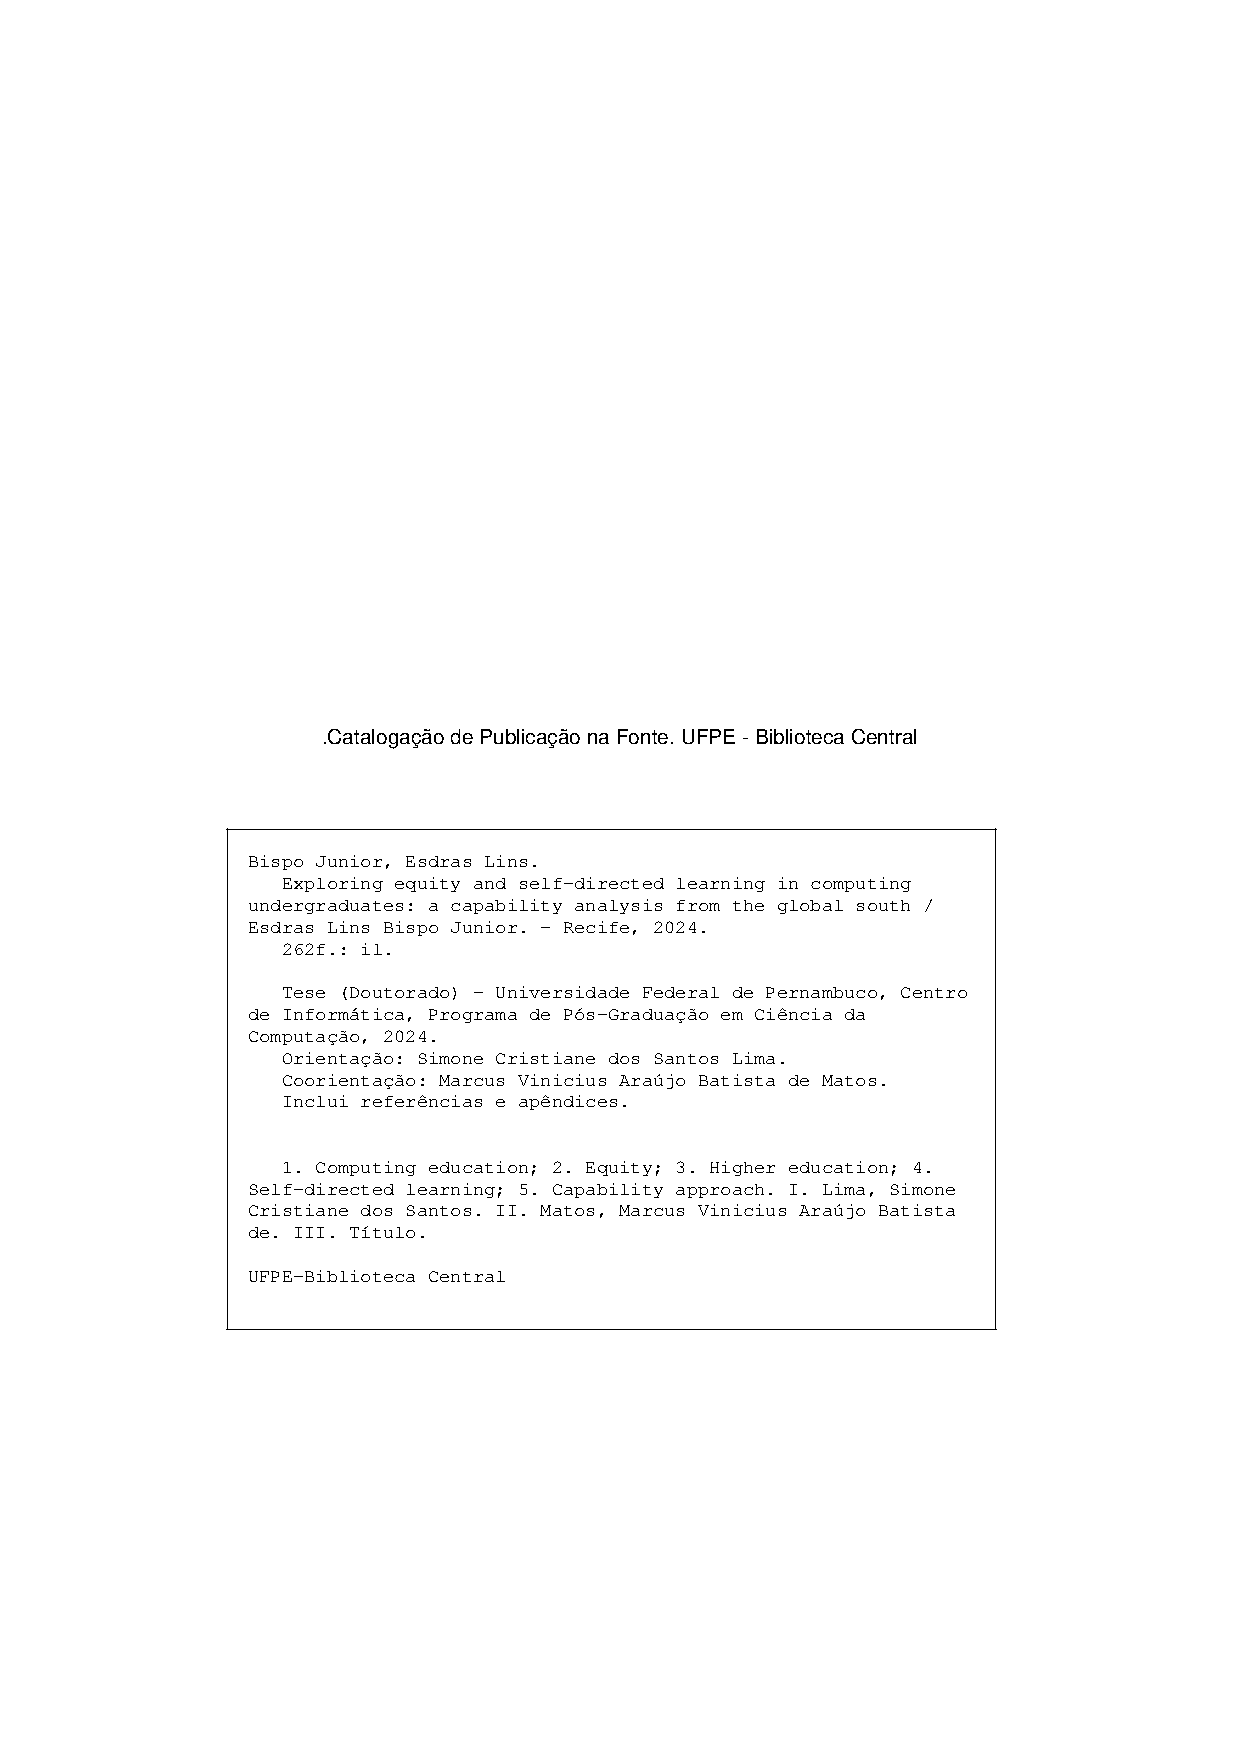
\includepdf[pages=-]{others/ficha_catalografica.pdf}

%\newpage
%\input{others/ata_defesa}
%a folha de aprovação deve ser um pdf que a secretaria encaminha sem assinaturas
%basta fazer upload na basta others e sobrescrever
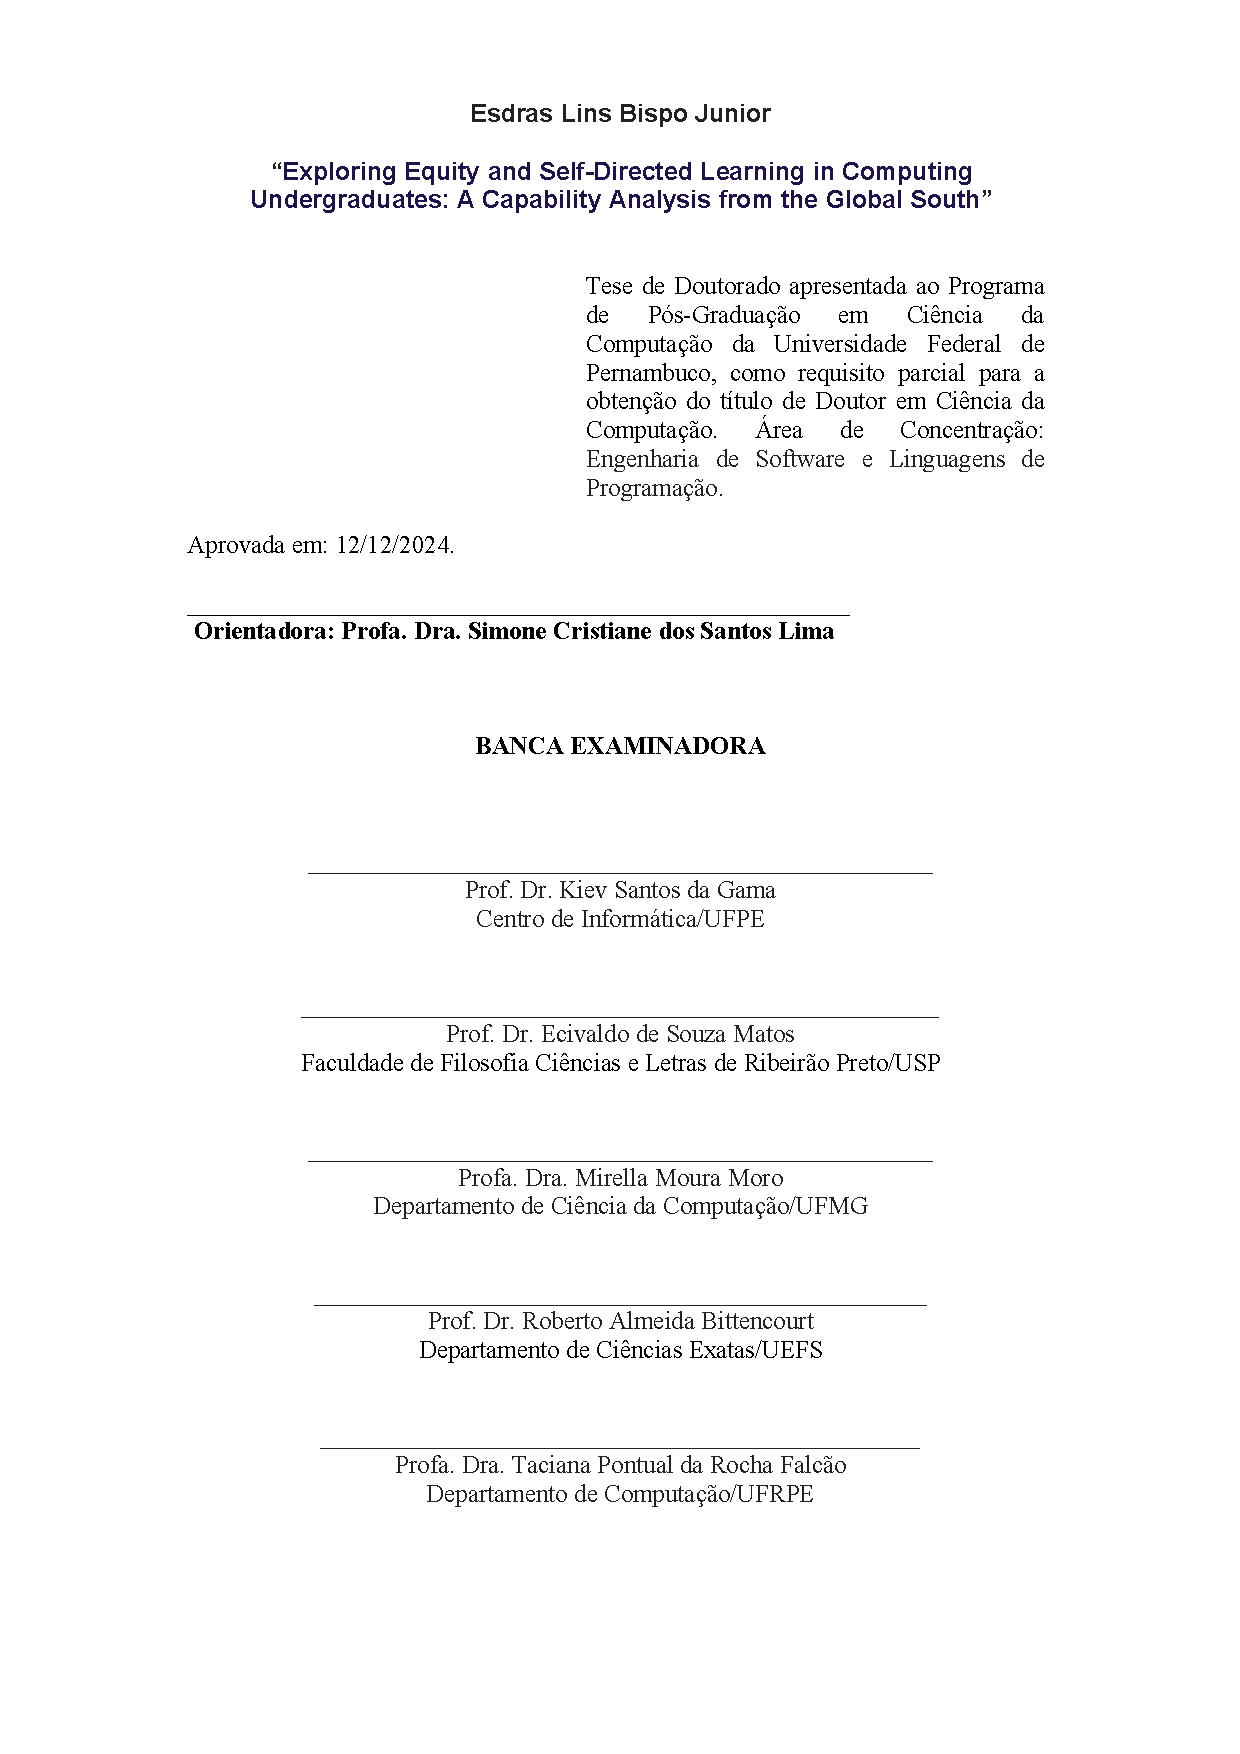
\includepdf[pages=-]{others/folha_aprovacao_final}

% ----------------------------------------------------------
% DEDICATÓRIA
% ----------------------------------------------------------
\begin{dedicatoria}
   \vspace*{\fill}
%   \centering
  % \noindent
   %\textit{\lipsum[2]} 
   I dedicate this work to all people around the world who believe in a fairer society
   %\vspace*{\fill}
\end{dedicatoria}
% ---

% ----------------------------------------------------------
% AGRADECIMENTOS
% ----------------------------------------------------------
\begin{agradecimentos}

Este trabalho é fruto de uma produção coletiva de muitas pessoas. É bem verdade que, de hoje em diante, este trabalho será atribuído como sendo de minha autoria. Porém, considero ser impossível ignorar ou desprezar, durante todo o processo (e até antes mesmo desse ciclo de formação), o quanto ele foi afetado através da influência da vida de várias pessoas.

É também bem triste perceber a minha incapacidade de poder fazer com justiça os meus agradecimentos neste momento. Como serei tentado a citar alguns nomes, ficam aqui já os meus sinceros agradecimentos a todos que contribuíram de alguma maneira para que tudo isso ocorresse. Sem vocês, com certeza, eu não teria condições de dar todos esses passos à frente.

Começo agradecendo ao Criador de todas as coisas. Àquele que criou todas as coisas e, ori\-ginalmente, disse que eram boas. Agradeço a Ele por todos os incômodos e pelas inquietações que me levaram a fazer uma pesquisa em Computação diferente das que eu normalmente já havia conduzido. Que "corra a retidão como um rio, e a justiça, como um ribeiro perene" (Profeta Amós 5.24).

Também agradeço à minha família, meu lar. O carinho e cuidado que recebo da minha esposa Ileamá e da minha pequena Larissa. Esse projeto foi uma decisão coletiva nossa e agradeço a Deus por ter essas duas companheiras de jornada que enchem a minha vida de alegria e esperança.

Também agradeço a todos os meus familiares, sempre me incentivando a explorar todo o potencial que existe em mim. Em especial: (i) aos meus irmãos Tarik e Polly. Amo vocês. Tenho certeza que papai e mamãe estariam orgulhosos do ser humano que nos tornamos hoje; e (ii) aos meus sogrinhos, Seu Ironcil e Tia Ianê... vocês moram de graça no meu coração.

Agradeço à Universidade Federal de Jataí (UFJ) que acreditou no meu trabalho e contribuiu efetivamente para que esse ciclo da minha formação fosse concluído. Ficam os agradecimentos especiais a todos os membros do Bacharelado em Ciências da Computação da UFJ.

Agradeço à Coordenação de Aperfeiçoamento de Pessoal de Nível Superior (CAPES) pela bolsa concedida durante a maior parte do doutorado. Tanto a bolsa no Brasil quanto no exterior foram fundamentais para que essa pesquisa fosse conduzida com a devida qualidade.

Agradeço aos meus dois orientadores: Profa. Simone Santos (Centro de Informática), Prof. Marcus Vinicius Matos (Brunel University London). Duas coisas são motivos de agradecimentos para vocês dois: confiança e paciência. Obrigado por confiarem no meu trabalho, nas minhas ideias e por permitirem essa caminhada junto a vocês. Obrigado pela paciência, principalmente nos momentos em que não havia muita clareza sobre o objeto de pesquisa, mas houve compreensão e o tempo necessário para que essa "filha" nascesse. Também devo registrar meus agradecimentos aos meus orientadores nos meses iniciais de chegada no programa de doutorado:  Prof. Sérgio Soares (Centro de Infomática), e Profa. Liliane Fonseca (Universidade Católica de Pernambuco). Agradeço por me acolherem e me acompanharem nesse primeiro momento de chegada por aqui.

Também expresso a minha gratidão a todos os colaboradores do Centro de Informática. 
Ter acesso ao laboratório 24 horas por dia e contar com toda a infraestrutura, com todo o apoio operacional e administrativo, trouxeram a mim paz e condições reais para que o doutorado pudesse chegar a esse momento final.

Também não poderia deixar de agradecer a todos os membros do Grupo NEXT de pesquisa pela caminhada e camaradagem nesses quatro anos de doutorado. Deixo meus agradecimentos especiais a dois "irmãos de orientação": Davi Maia e André Ribeiro. Agradeço pelas várias discussões e boas reflexões sobre Educação em Computação e sobre a vida. Força e sucesso! Vamos que vamos.

Agradeço a todos os meus companheiros de luta de laboratório da APG. Em especial, a David Cavalcanti, Yeda Lima e Susi Vila Nova. Dividir o lab e a dureza da caminhada de uma pós-graduação com vocês tornou essa jornada menos dura. Obrigado pelo companheirismo de vocês.

Ficam também os meus agradecimentos à toda a comunidade de Educação em Computação no Brasil, em especial à CEduComp-SBC. Ser parte dessa comunidade e de sua história é um motivo de imensa alegria para mim. Deixar alguns nomes preciosos fora desses agradecimentos é difícil (e deixarei, infelizmente). Mas eu tenho que fazer um registro em especial ao meu amigo cientista Robson Feitosa. Bom poder caminhar essa jornada doutoral ao seu lado, meu querido. Um abraço pra todo esse povo bonito do IFCE Crato.

Tenho que deixar um registro especial para esse meu casal de padrinhos: Kathleen Vasconcelos e Jônatas Abreu. As nossas muitas conversas sobre família, Reino de Deus e justiça nos levaram ocasionalmente aos textos de Amartya Sen. Muito obrigado pelas conversas e pela boa compa\-nhia nessa caminhada. Tenho certeza absoluta que a construção do meu referencial teórico não existiria nesse formato sem as boas risadas e discussões importantíssimas sobre equidade.

Também agradeço aqui a três comunidades que acolheram a mim e à minha família com grande carinho na Inglaterra. Primeiro à toda comunidade internacional de estudantes evangélicos, mas especialmente aos brasileiros "sempre ABUenses" que vivem por essas bandas: (i) meu agradecimento a Marcos Vinícius, Priscila, e Aurora que receberam tão carinhosamente em sua casa em Uxbridge em um momento tão difícil de perda familiar... meu muito obrigado de coração; (ii) também agradeço ao carinho de Miguel e Giovanna que também abriram carinhosamente a casa deles para receberem a minha família em Londres; e (iii) aos demais que dividiram momentos de conversas, risos, e apreensões (especialmente Henrique e família) e aquele churrasco brasileiro que nunca é demais [risos] (Juliana Noronha e família).

Em segundo, agradeço à toda a comunidade do Exército da Salvação em Cradley Heath. Embora estrangeiros, fomos recebidos como se não fôssemos nessa comunidade. Meu agrade\-cimento especial é para Heatham por todo o seu carinho e cuidado que certamente vem do Reino dos Céus. E, por fim, também agradeço à toda a comunidade do \textit{Dudley \& Sandwell Table Tennis Club}, em especial a Chris Dunkley por me receber tão carinhosamente nos treinos no \textit{African-Caribbean Community Network} e nos jogos na liga inglesa de tênis de mesa.

\end{agradecimentos}



% ----------------------------------------------------------
% EPÍGRAFE

%Epígrafe: Elemento opcional e sem título em que o (a) autor (a) apresenta uma citação relacionada ao assunto tratado no trabalho. Deve ser elaborada conforme a ABNT-NBR 10520 (Citações). As citações de até três linhas devem estar entre aspas duplas e as citações com mais de três linhas devem ser destacadas com recuo de 4 cm da margem esquerda, com letra menor que a do texto e sem as aspas. A fonte da citação deve aparecer na lista de referências.
% ---------------------------------------------------------
\vspace*{10cm}
% \begin{citacao}
% Texto texto texto texto texto texto texto texto texto texto texto texto texto.Texto texto texto texto texto texto texto texto texto texto texto texto texto texto texto texto texto texto texto texto texto texto texto texto texto texto texto texto texto texto texto texto texto texto texto texto texto texto texto texto texto texto texto texto texto texto texto texto texto texto texto texto texto texto texto texto texto texto texto texto texto texto \cite{manualufpe2020}.
% \end{citacao}

    \vspace*{5cm}
	
    ''But so shall it not be among you: but whoever will be great among you, shall be your minister: and whoever of you will be the most chief, shall be servant of all'' 
  \begin{flushright}
      \textbf{Jesus Christ} (Mark 10:43,44)
  \end{flushright}
	
\newpage

% resumo em português
% \begin{resumo}[Resumo] 

% Texto texto texto texto texto texto texto 
% % \noindent %- o resumo deve ter apenas 1 parágrafo e sem recuo de texto na primeira linha, essa tag remove o recuo. Não pode haver quebra de linha.

%  \vspace{\onelineskip}
    
%  \noindent
%  \textbf{Palavras-chaves}: Texto. Texto. Texto. Texto. Texto.Texto.
% \end{resumo}



% resumo em inglês
\begin{resumo}[Abstract]
%\begin{otherlanguage*}{english}

\gls{CSE} concerns the reflection of equitable variables like gender, race/ethnicity, socioeconomic status  and culture. However, addressing how to balance different sources of inequities is still an open challenge. Although \gls{CAPE} framework can map most of the main variables to an equity analysis, the concept of capacity is strongly related to resources, ignoring some essential aspects relative to the real opportunities for a computing student. Another framework that can address this problem is the \gls{CA}, having the freedom of being educated is one of the aims of this perspective. In this direction, active learning and \gls{SDL} can potentialize the freedom of \gls{CSE} students, promoting more autonomy and crucial soft skills in our complex society. \gls{SDL} is a potential equitable practice, but there are open challenges to consider regarding when and how to use it. Understanding better how \gls{SDL} effectively occurs in \gls{CSE} students can also contribute to comprehending the potentiality of active learning in terms of capabilities. Thus, this doctoral research investigated how do \gls{CSE} students conduct their \gls{SDL} in developing countries from the \gls{CA} lens. Three \glspl{RG} help to address this question in a qualitative approach: (\gls{RG}1) understanding how \gls{CSE} students build their \gls{SDL} trajectories in developing countries; (\gls{RG}2) mapping the main elements of \gls{SDL} capabilities observed in \gls{CSE} students in developing countries; and (\gls{RG}3) recommending guidelines to (\gls{CSE}) educational stakeholders concerning how to consider effectively equity issues and active learning from the \gls{CA} lens.  The results are structured over the perceptions of two \gls{CSE} Brazilian undergraduates about their \gls{SDL} trajectories, being each one from the lowest and highest \gls{SES} of their class, respectively. Interviews and other data sources helped to better situate the findings. The doctoral contributions were in (i) the use of \gls{CA} as an equity theoretical framework in computing research, and \gls{CEd}, (ii) the proposition of a new concept called \gls{SDL} capabilities, and (iii) a pragmatic instantiation of equity discussions in \gls{CSE} (beyond other scientific contributions to Computing and Education in a general way).

   \vspace{\onelineskip} 
 
   \noindent 
   \textbf{Keywords}: Computing Education. Equity. Higher Education. 
   \\ \mbox{ } \hspace{48pt} Self-Directed Learning. Capability Approach.
 %\end{otherlanguage*}
 \end{resumo}


% ----------------------------------------------------------
% LISTA DE FIGURAS
% ----------------------------------------------------------
\pdfbookmark[0]{\listfigurename}{lof}
\listoffigures*
\cleardoublepage


% ---
% LISTA DE CÓDIGOS FONTES
% ---

\pdfbookmark[0]{\lstlistingname}{lol} % caso não tenha quadros, comente esta linha 
\counterwithout{lstlisting}{chapter}



% Altera o nome padrão do rótulo usado no comando \autoref{}
\renewcommand{\lstlistingname}{Código Fonte}

% Altera o rótulo a ser usando no elemento pré-textual "Lista de código"
\renewcommand{\lstlistlistingname}{Lista de códigos}

% % Configura a ``Lista de Códigos'' conforme as regras da ABNT (para abnTeX2)
% \begingroup\makeatletter
% \let\newcounter\@gobble\let\setcounter\@gobbletwo
%   \globaldefs\@ne \let\c@loldepth\@ne
%   \newlistof{listings}{lol}{\lstlistlistingname}
%   \newlistentry{lstlisting}{lol}{0}
% \endgroup

% \renewcommand{\cftlstlistingaftersnum}{\hfill--\hfil}

% \let\oldlstlistoflistings\lstlistoflistings
% {
% \let\oldnumberline\numberline
% \newcommand{\algnumberline}[1]{Código Fonte~#1~\enspace--~\enspace}
% \renewcommand{\numberline}{\algnumberline}

% \begin{KeepFromToc}
% \lstlistoflistings
% \end{KeepFromToc}
% }
% \cleardoublepage

% % ---
% % LISTA DE QUADROS
% % ---
\pdfbookmark[0]{\listofquadrosname}{loq} % caso não tenha quadros, comente esta linha 
\listofquadros* % caso não tenha quadros, comente esta linha 
\cleardoublepage



% ----------------------------------------------------------
% LISTA DE TABELAS
% ----------------------------------------------------------

\pdfbookmark[0]{\listtablename}{lot}
\listoftables*
\cleardoublepage


        
  
% ----------------------------------------------------------
% LISTA E ABREVIATURAS E SIGLAS
% ----------------------------------------------------------
% \printglossary[type=\acronymtype,title={\listadesiglasname},nonumberlist]
% \printglossaries
% compile uma vez com o comando \printglossaries e depois compile novamente com o comando \printglossaries comentado para as páginas glossário e siglas serem ocultadas.

% ----------------------------------------------------------
% LISTA E ABREVIATURAS E SIGLAS
% ----------------------------------------------------------
%\setglossarystyle{modsuper}
%\printnoidxglossary[style=modsuper,type=\acronymtype,title={\listadesiglasname},nonumberlist]
\printnoidxglossary[style=super,type=\acronymtype,title={\listadesiglasname},nonumberlist]
% \printglossary[style=super, type=\acronymtype]
\cleardoublepage



% ----------------------------------------------------------
% LISTA DE SIMBOLOS
% ----------------------------------------------------------
%


% ---

% ---
% inserir lista de símbolos
% ---
\begin{simbolos}
  \item[$ \gamma $] Letra grega Gama
  %\item[$ \Lambda $] Lambda
  %\item[$ \zeta $] Letra grega minúscula zeta
  \item[$ \in $] Pertence
%  \item[$ \infty$] Infinito
%  \item[$ \ge$] Maior ou Igual
  \item[$ \delta$] Delta
  \item[$ \theta$] Teta
  \item[$ \sigma$] Sigma
  \item[$ \mu$] Mi
  
\end{simbolos}
% ---




% ----------------------------------------------------------
%


% ---

% ---
% inserir lista de símbolos
% ---
\begin{simbolos}
  \item[$ \gamma $] Letra grega Gama
  %\item[$ \Lambda $] Lambda
  %\item[$ \zeta $] Letra grega minúscula zeta
  \item[$ \in $] Pertence
%  \item[$ \infty$] Infinito
%  \item[$ \ge$] Maior ou Igual
  \item[$ \delta$] Delta
  \item[$ \theta$] Teta
  \item[$ \sigma$] Sigma
  \item[$ \mu$] Mi
  
\end{simbolos}
% ---






% ----------------------------------------------------------
% SUMÁRIO
% ----------------------------------------------------------
\pdfbookmark[0]{\contentsname}{toc}
\tableofcontents*
% \begingroup\intoctrue
% \tableofcontents*
% \endgroup
\cleardoublepage

% \setcounter{page}{13}
\setcounter{tocdepth}{2}
\setcounter{table}{0}




% ----------------------------------------------------------
% ELEMENTOS TEXTUAIS
% ----------------------------------------------------------
\textual


% referencie todos os arquivos de capítulos aqui, fique a vontade para
% fazer a sua organização de diretórios

  % exemplo de organização interna de um capítulo separando por mais de um arquivo

  \chapter{Introduction}
\label{chap:intro}

This chapter is divided into fivesections. Section \ref{intro-sec:mot-prob} presents the general problem that motivates this project. Section \ref{intro-sec:overview} delineates an overview of the main ideas concerning this research. Section \ref{intro-sec:rel-computing} highlights the research relevance to computing educators. Section \ref{intro-sec:sum-contributions} summarizes the main research contributions. And, at last, Section \ref{intro-sec:goals-pres} elicits the research goals and points out the remainder of this thesis.
  \section{Motivation Problem}
\label{intro-sec:mot-prob}

Imagine three children and one problem. You must decide who (Anne, Bill, or Carla) should get a mini keyboard built essentially from Arduino components. Anne claims the mini keyboard because she is the only one capable of playing it (and the others do not deny this fact). In her vision, denying the mini keyboard to the only person who really knows how to play it would be unfair. If this were all you knew, you would have a solid reason to give Anne the mini keyboard. 

Now, imagine a second scenario. Bill claims the mini keyboard because he is the only one so poor that he has no toys. The mini keyboard allows him to play (and the others admit they are more prosperous than him and dispose of a good variety of toys). If you listened only to Bill, you have a solid reason to give the mini keyboard to him. 

Imagine, at last, the third scenario. Carla says that she built the mini keyboard with her own hands. She worked hard for many months for this. And only when Carla finished making it, the other children claimed the mini keyboard. If you listened only to Carla, it would be plausible to agree that she should be able to use something she made.

These analogies are an adaptation of Amartya Sen’s example (\citeyear{sen:2009}), identifying the difficulties of choosing the fairer option. Depending on your philosophical basis (e.g., utilitarianism, libertarianism, economic egalitarianism), the decision may differ in each case but is still ``obvious'' from each viewpoint. We can transpose this problem to \acrfull{CSE}. How could \gls{CSE} stakeholders (e.g., professors, educational managers) appropriately consider the various equity issues that emerge from a diverse class? How could they balance race, gender, and socioeconomic issues, for instance? How can this be done in the active learning context, where student engagement is highly expected?

It is important to highlight two essential contexts that benefited from this deepened discussion about equity. First, the Brazilian community of computing education research gained strength from 2019 with the collective articulation of the \gls{GIEC}, leading to the emergence of the \gls{CEduComp} of the \gls{SBC} in 2023. Investigating equity and active learning in computing contributes to the formation of more humanized computing research in Brazil, also favoring the promotion of a critical mass of computing researchers in \acrfull{CEd}.

Second, there is a worldwide ongoing movement that is delegitimizing efforts towards \gls{DEI} agenda. This movement signals reforming the aims of education and, consequently, \gls{CEd} \cite{tedre:2018}. Deepening this discussion about equity not only contributes to computing research but to a better understanding of this agenda as a whole, which is of high importance in this context of political polarization and the uncertainty about the future of \gls{DEI} policies and affirmative actions around the world \cite{malcom:2024}.


  \section{Overview}
\label{intro-sec:overview}

\gls{CSE} concerns the reflection of equitable variables. Various works in this area approach equity issues like gender \cite{kim:2011}, race/ethnicity \cite{nakajima:2024}, socioeconomic status \cite{parker:2018}, and culture \cite{arawjo:2021}. Equity and diversity also used to be two sides to a story in \acrfull{CEd}, allowing us to see the same problem from these two perspectives \cite{lewis:2019}. However, addressing how to balance different sources of inequities is still an open challenge.

A framework to address this problem is CAPE \cite{fletcher:2021}. This stands for \acrfull{CAPE}. This framework proposes a lens for assessing equity not only in \gls{CSE} but in \gls{CEd} as a whole. Although \gls{CAPE} can map most of the main variables to an equity analysis, the concept of capacity is strongly related to resources, ignoring some essential aspects relative to the real opportunities for a computing student.

Another framework that can address this problem is the \acrfull{CA} proposed originally by Amartya Sen (\citeyear{sen:1992}) and improved by Melanie Walker (\citeyear{walker:2006}) for education purposes. This approach allows us to identify not only the resources that are supposed to be absent in inequity scenarios but also map the capabilities that cannot possibly be developed by a student. Other education fields use the capabilities approach (e.g., Geography \cite{walkington:2018}, but \gls{CEd} still has explored its potentialities marginally.

The \gls{CA} is a theoretical framework based upon two normative claims: (i) the freedom to achieve well-being is of primary moral importance, and (ii) the understanding of well-being is directly related to people’s capabilities and functionings. The freedom of being educated is one of the aims of this perspective, understanding it as a part of the broad problem of liberating people for a fulfilling life.

In this direction, active learning can potentialize the freedom of \gls{CSE} students, promoting more autonomy and crucial soft skills in our complex society. Pedagogical frameworks and methodologies like andragogy \cite{ellis:2002}, problem-based learning \cite{santos:2021}, and peer instruction \cite{bispojr:2021} somehow develop the idea of active learning in this area. These approaches strongly dialog with the constructivism theory (which asserts the students “construct knowledge rather than merely receive and store knowledge transmitted by the teacher” \cite[p.~45]{ben-ari:2001} and, by consequence, with self-directed learning \cite{mccartney:2016}. 

In the \gls{STEM} context, active learning pedagogies have been effective in promoting the increase of learning outcomes \cite{prince:2004}. However, collaborative pedagogies in the \gls{CSE} context has led to marginalization \cite{lewis:2015} like over-dominance concerning student participation. \acrfull{SDL} is a potential equitable practice \cite{anderson:2022}, but there are open challenges to consider regarding when and how to use it \cite{brookfield:1993}. Understanding better how \gls{SDL} effectively occurs in \gls{CSE} students can also contribute to comprehending the potentiality of active learning in terms of capabilities.

In developing countries, other challenges emerge. Beyond the potential inequity sources that emerged from natural diversity in the classroom (e.g., gender, race), structural barriers deepen the situation (e.g., socioeconomic status, poverty). In African countries, for instance, it used the \gls{CAPE} framework to analyze equity issues in \gls{CEd} \cite{tshukudu:2023}. Although the authors highlight the strengths of its use, they also point out some limitations: 
\begin{citacao}
    ``The \gls{CAPE} framework helps map the progression from 'Capacity for' to 'Experience of' computer science education as a route to equity, but in order to support development in low and middle income countries, it may be helpful to have the capacity level finely grained'' \cite[p.~1]{tshukudu:2023}.
\end{citacao}
Maybe the capability approach can help to fill some gaps during equity analysis using only the \gls{CAPE} framework.

 In this way, the proposed research will help to establish a process to identify the crucial \gls{CSE} capabilities in the context of self-directed learning in developing countries. The fundamental presupposition is to ensure fair and equitable \gls{CSE}, mainly in the Global South. However, how do we propose the actions and policies needed to mitigate and, if possible, eliminate the sources of unfairness from an interrelated and multifactorial perspective of equity issues (e.g., race, gender, socioeconomic status)? One way is to assess the educational scenario from the capabilities approach.
  \section{Relevance to Computing Education Practitioners}
\label{intro-sec:rel-computing}

It is possible to highlight three directions concerning the relevance of this \gls{Ph.D.} to \gls{CEd} practitioners. First, this thesis contributes to forging awareness about equity issues in \gls{CEd} \cite{bispojr:2022-educomp}. \gls{CEd} practitioners usually do not have in their previous formation an adequate space to discuss and deepen the discussion about equity issues in computing contexts. Writing materials and papers contextualizing into \gls{CEd} allows them to visualize the applicability in their professional places better.

Second, this thesis contributes to the provisioning of constructs to analyze equity in a computing class \cite{bispojr:2024-nmp}. It is essential to increase awareness to promote the intrinsic will towards an educational change. But this awareness can be fruitless if \gls{CEd} practitioners cannot verbalize it using a set of equity constructs. \gls{CA} provides this set, and, during this thesis, it is possible to realize how to identify each one of them inside a situated \gls{CEd} context.

Third, and last, refers to a pragmatic instantiation of equity discussions in \gls{CSE} (mainly in \cite{bispojr:2024-online-lab}). The proposition of a set of guiding questions to orientate an initial equity analysis for an Engineering collective decision-making of professors serves this purpose, provoking them not only to change their standing but also change their actions through the following of this propositional pathway. These recommendations can easily be transposed from engineering education to \gls{CEd}.
                
  \section{Summary of Research Contributions}
\label{intro-sec:sum-contributions}

This is the list of main research contributions of the \gls{Ph.D.} period:
\begin{enumerate}
    \item[(i)] the use of \acrfull{CA} as an equity theoretical framework in computing research, and \acrfull{CEd} mainly;
    \item[(ii)] the proposition of a new concept called \acrfull{SDL} capabilities, providing a lens to assess equity in active learning scenarios;
    \item[(iii)] a pragmatic instantiation of equity discussions in \acrfull{CSE};
    \item[(iv)] relevant \gls{CEd} publications \cite{bispojr:2024-isdls,bispojr:2024-nmp,bispojr:2024-urca,   feitosa:2024,cavalcanti:2024,pereira:2024,melo:2024-horizontes,boaventura:2024-sbgames,boaventura:2023,esmeraldo:2023,freire:2023-rsc,freire:2023-encompif, santos:2022,bispojr:2022-educomp,esmeraldo:2022,bispojr:2021,bispojr:2021-educomp,bispojr:2021-wei,bispojr:2020-tec}, and
    \item[(v)] other relevant computing publications \cite{bispojr:2024-online-lab,cavalcanti:2024-ieee,bispojr:2023-edi,bispojr:2023-rbie,sansil:2023,bispojr:2022-snee,lima:2022}.
\end{enumerate}

% \fbox{
%     \begin{minipage}[htb]{0.9\textwidth}
%         \vspace{0.3cm}
                
%         \colorbox{gray!30}{% create a colored box
%             \makebox[0.975\textwidth][l]{% center the text on the page
%                 \ \ \textbf{Further Writing}
%             }
%         }

%         \vspace{0.1cm}
        
%         \begin{itemize}
%             \item Scientific works in Computing Education (list of papers), Computing in Education (list of papers), and Related Areas (list of papers).
%             \item Scoping study about equity and active learning in computing education.
%             \item Positionality essay using a rigorous reflexivity framework.
%             \item Chapter 6 as a didactic introduction to qualitative research in Computing Education.
%             \item Others???
%         \end{itemize}

%         \vspace{0.25cm}
        
%     \end{minipage}
% }

  \section{Goals and Presentation}
\label{intro-sec:goals-pres}

The \gls{MRQ} of this \gls{Ph.D.} thesis is 
\begin{itemize}
    \item[\textbf{(\gls{MRQ})}] ``How do \gls{CSE} students conduct their \gls{SDL} in developing countries from the \gls{CA} lens?''.
\end{itemize}
Three research goals (\glspl{RG}) help to address this question: 
\begin{itemize}
    \item[\textbf{(\gls{RG}1)}] understanding how \gls{CSE} students build their \gls{SDL} trajectories in developing countries; 
    \item[\textbf{(\gls{RG}2)}] mapping the main elements of \gls{SDL} capabilities observed in \gls{CSE} students in developing countries; and
    \item[\textbf{(\gls{RG}3)}] recommending guidelines to (\gls{CSE}) educational stakeholders concerning how to consider effectively equity issues and active learning from the \gls{CA} lens.
\end{itemize} 

From this point, the thesis will be written in the first person where applicable. My philosophical basis of research allows me to seek methodological rigor without writing it in the third person, which is usually necessary when looking for more objectivity. It is possible to guarantee objectivity without forcing supposed neutrality (\citeauthor{saviani:1994}, \citeyear{saviani:1994}, p.~76; \citeauthor{bispojr:2022-educomp}, \citeyear{bispojr:2022-educomp}). I will develop this idea better in Chapter \ref{chap:reflex-essay}.

The remainder of this thesis is divided as follows. Chapters \ref{chap:sdl} e \ref{chap:equity} present the two central concepts of this thesis: self-directed learning and equity, respectively. Chapter \ref{chap:rel-work} identifies and discusses the related work through a mapping review. Chapter \ref{chap:reflex-essay} positions a reflexivity essay, providing my assumptions and worldview during my \gls{Ph.D.} journey. Chapter \ref{chap:res-methodology} establishes the rationale for the methods, discussing their appropriateness in this research. Chapter \ref{chap:res-design} structures the research design, pointing out the specificities concerning the method application. Chapter \ref{chap:results} presents the results obtained from the data collection. Chapter \ref{chap:discussion} discusses the results, searching for answers to the research questions. Chapter \ref{chap:final-remarks} summarizes the final remarks, shimmering the main findings and potential future works. Finally, Appendix \ref{chap:appendix-a} provides the trajectory of my latest published research and other essential artifacts used during this research (Appendixes \ref{chap:socio-quest}, \ref{chap:appendix-scripts}, \ref{chap:data-charting}, \ref{chap:interview-excerpts}, and \ref{chap:pbl-see-charts}).


  
\chapter{Self-Directed Learning}
\label{chap:sdl}

There are many ways to refer to self-directed learning (\gls{SDL}). In the middle of a definition’s diversity, I will adopt a genealogical perspective to choose an appropriate definition for \gls{SDL}. Three seminal authors are essential in this approach: Cyril Houle, Alen Tough, and Malcolm Knowles. I will explain in more detail the contributions of each of them to reach an adequate \gls{SDL} definition.

Houle’s work entitled ``Inquiring Mind'' (\citeyear{houle:1961}) introduced the first concerns that would be important to reach a future SDL concept. Brockett and Donaghy (\citeyear{brockett:2005}) narrate Houle’s study with 22 adult learners presented in this work:
\begin{citacao}
    ``He categorized these learners in three different ways based how they viewed the ‘purposes and values of continuing education’: goal-oriented, activity-oriented, and learning-oriented. It was the latter of these groups that was of particular interest relative to self-directed learning. The learning-oriented adult was described as an adult who engages in learning purely for ‘the desire to know’. Here, Houle draws parallels to self-directed learning''.
\end{citacao}

The “learning-oriented adult” category contained an incipient \gls{SDL} definition. From this context, Allen Tough and Malcolm Knowles would take important steps to a more solid definition. Tough and Knowles are former doctoral students of Houle and deepened this discussion, advancing toward a better \gls{SDL} definition. Tough (\citeyear{tough:1967}) established a similar \gls{SDL} concept as follows:
\begin{citacao}
    “When an individual decides that he wants to learn certain information, knowledge or skill, he often seeks a professional instructor to tell him how to proceed and to supervise his learning. However, instead of turning most of the responsibility over to a professional teacher, the individual may decide to act as his own teacher, and assume the primary responsibility for planning, initiating, and conducting the learning project. Such behavior can be called self-teaching and the person learning in this manner can be called a \underline{self-teacher}” (author’s emphasis).
\end{citacao}

Self-teaching was one of the first definitions to touch slightly on the \gls{SDL} concept used in this text. Some essential aspects of \gls{SDL}, like planning, initiating, and conducting the own learning, are related in this definition. Although it mentions these aspects, this definition does not have sufficient granularity regarding the main phases of the whole learning process.

At last, Knowles (\citeyear{knowles:1975}, p.~18) defined \gls{SDL} in a more specific way, covering the main phases of the learning process:
\begin{citacao}
    “In its broadest meaning, ‘self-directed learning’ describes a process in which individuals take the initiative, with or without the help of others, in diagnosing their learning needs, formulating learning goals, identifying human and material resources for learning, choosing and implementing appropriate learning strategies, and evaluating learning outcomes”.
\end{citacao}

The \gls{ISSDL} uses two definitions as references. During the 33rd \gls{ISSDL} Symposium, the \gls{ISSDL} board developed a more concise \gls{SDL} definition, “thereby helping scholars to differentiate what is and is not \gls{SDL}-related practice, research, and theory” \cite{issdl:2020}.  This definition asserts, “\gls{SDL} is an intentional learning process that is created and evaluated by the learner”. However, \gls{ISSDL} also adopts Knowles’ definition as a more extensive version. Due to the importance of the \gls{ISSDL} decision, I use Knowles’ definition as the basis for this work and the \gls{ISSDL} board’s short definition if it is necessary to refer to \gls{SDL} synthetically. I created Figure \ref{fig:sdl-process} to present the \gls{SDL} process from Knowles’ definition schematically.

\begin{figure}[ht!]
\centering

\caption{\textmd{\acrshort{SDL} process from Knowles’ definition schematically.}}
\label{fig:sdl-process}
\fcolorbox{gray}{white}{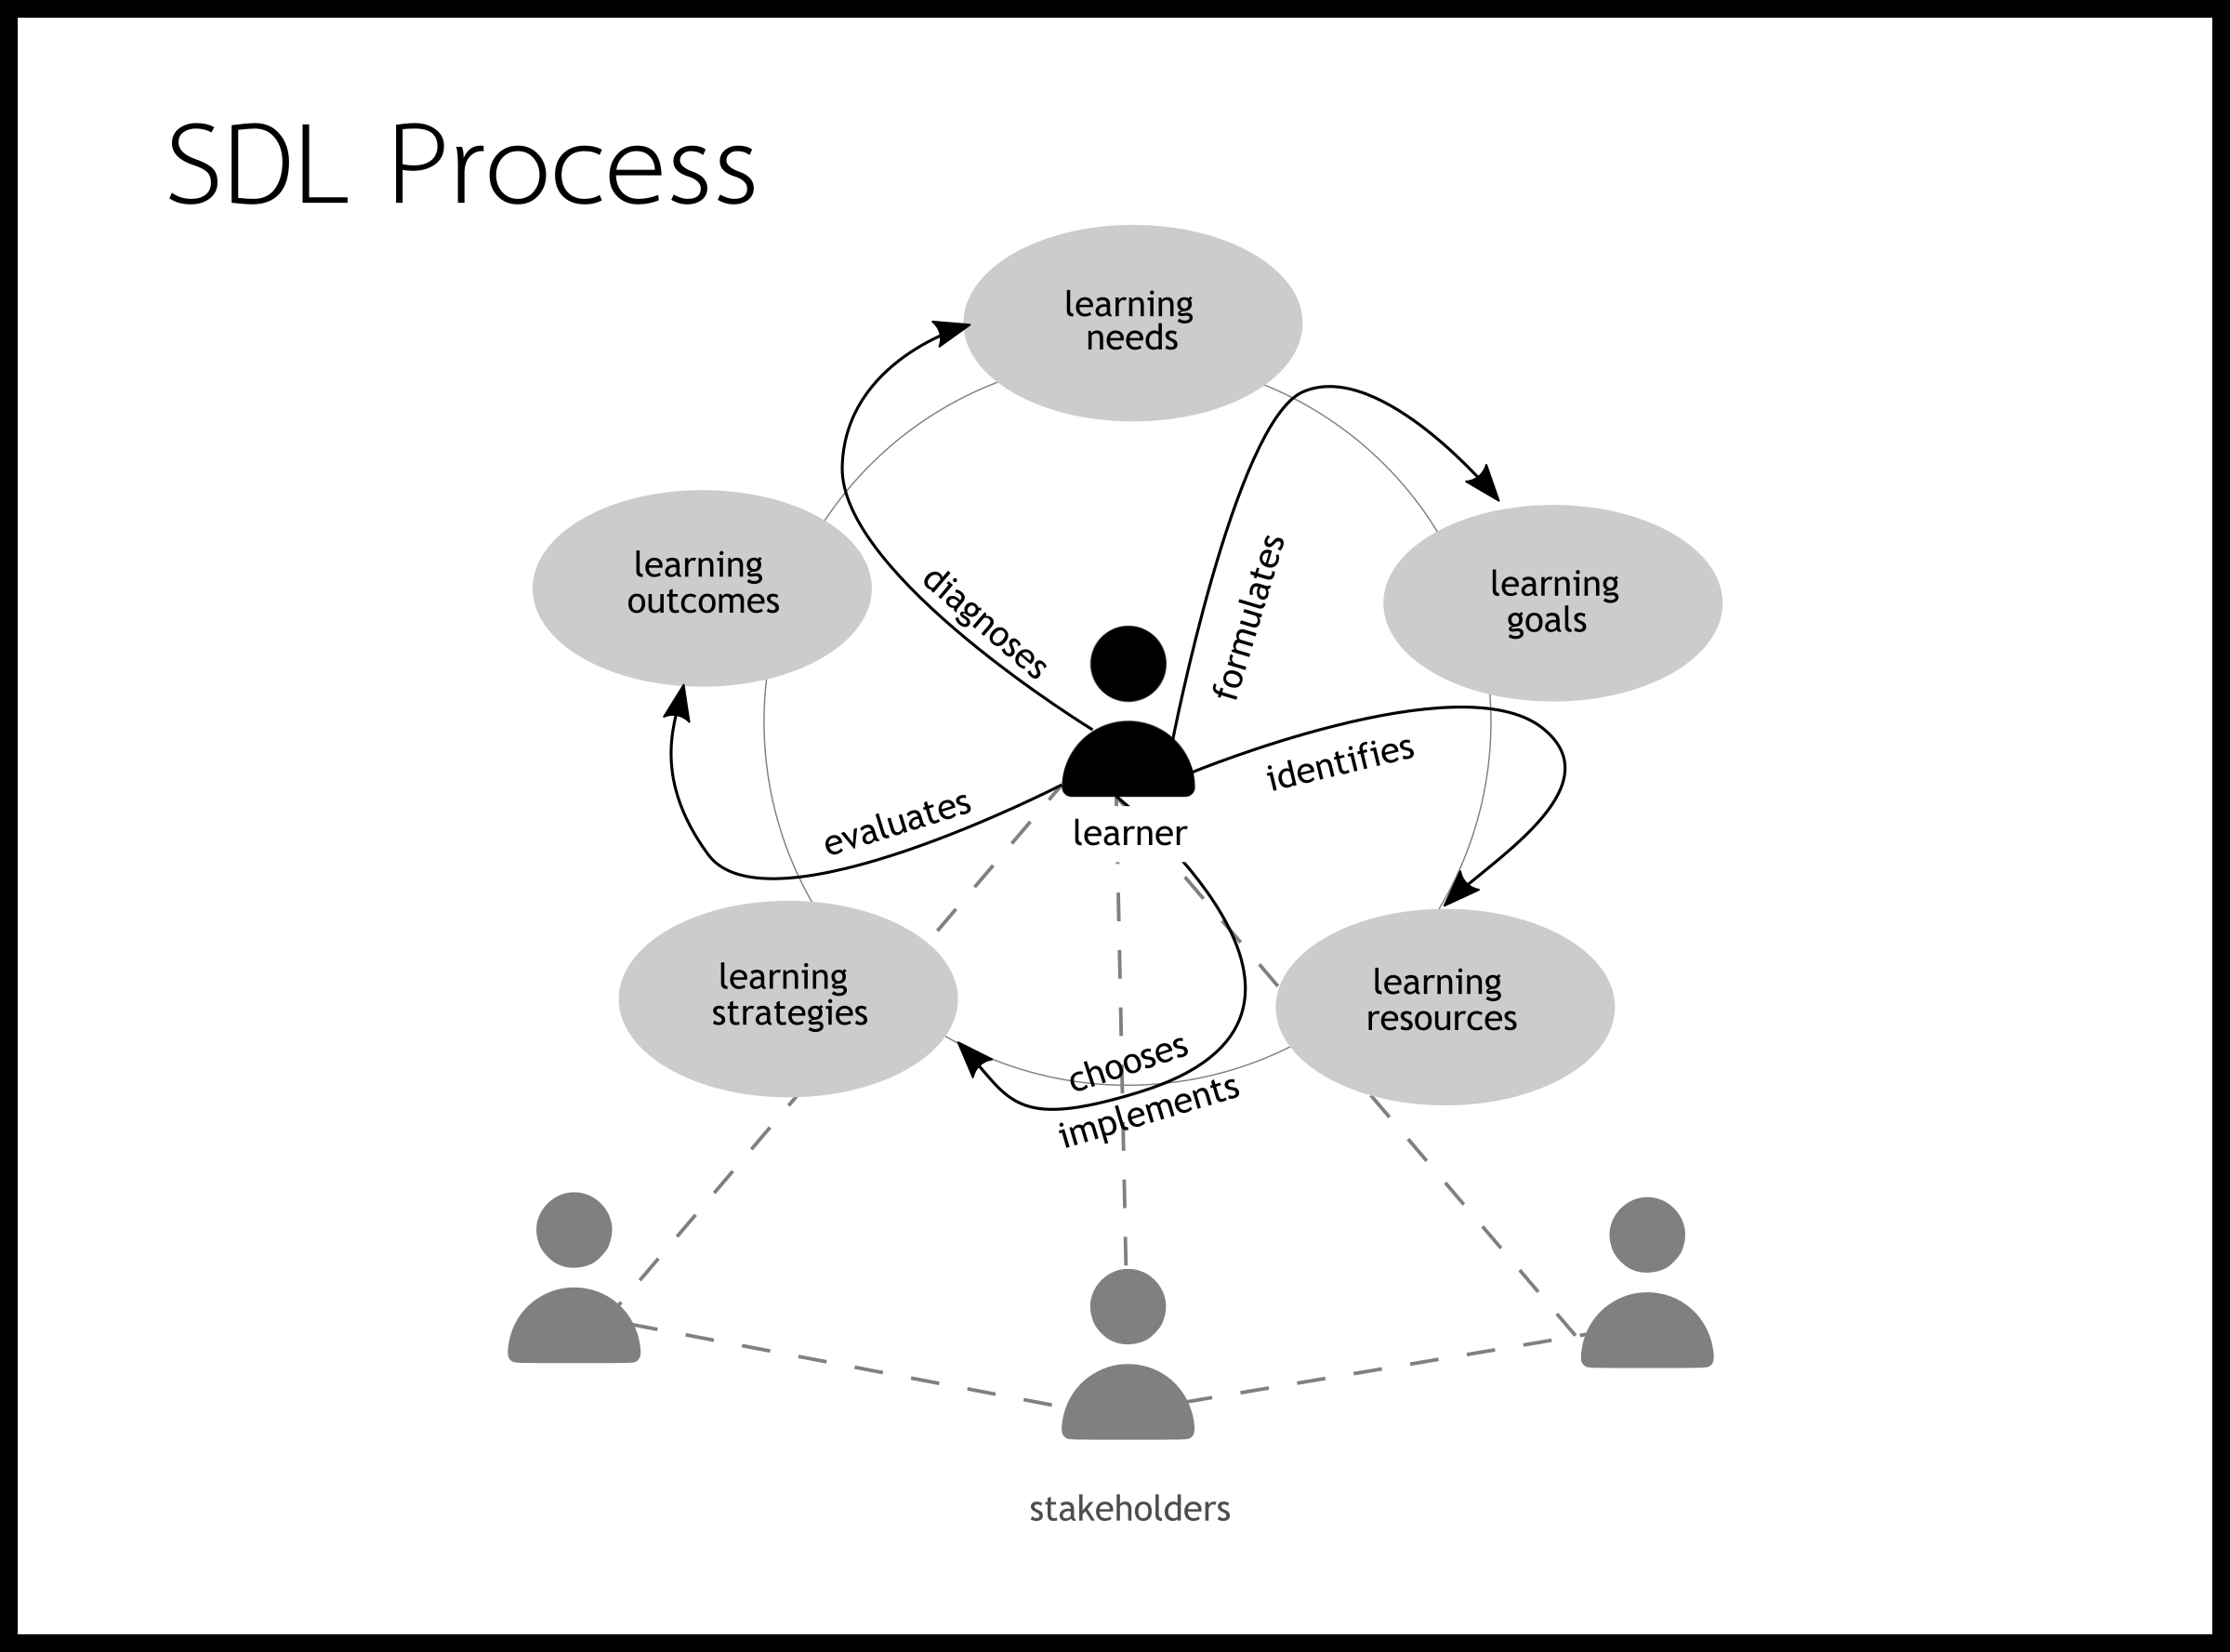
\includegraphics[width=0.9\textwidth]{images/chapter-02/sdl-process.png}}

\par\medskip\ABNTEXfontereduzida\selectfont\textbf{Source:} Created by the author (2024).
%\citeauthor{manualufpe2020} (\citeyear{manualufpe2020}) \par\medskip
\end{figure}

Throughout this chapter, I present \gls{SDL} in various aspects. Section \ref{sdl-sec:goals} points out the different \gls{SDL} goals, considering which philosophical framework the research uses as a reference. Section \ref{sdl-sec:models} enumerates the many ways to model the \gls{SDL} process, highlighting these models’ potentialities and weaknesses. Section \ref{sdl-sec:relations} establishes some relations from the \gls{SDL} concept into some approaches like andragogy, problem-based learning, and self-regulated learning. And, at last, Section \ref{sdl-sec:challenges} presents some existing research challenges involving \gls{SDL}, situating which one this research addresses.

\section{SDL Goals}
\label{sdl-sec:goals}

It is possible to arrange the \gls{SDL} kinds from the underlying philosophical position \cite[p.~206]{caffarella:1987}. I created three classes based on skill improvement (Section \ref{sdl-goal-ss:skill}), critical reflection (Section \ref{sdl-goal-ss:reflection}), and social emancipation (Section \ref{sdl-goal-ss:emanc}). Each class depends on the learner goal\footnote{There are other SDL classifications made by \citeonline{caffarella:1987} and \citeauthoronline{merriam:2007} (\citeyear{merriam:2007}, p.~107-110). The need to create another one is because the first is more comprehensive than what I need for the purposes of this work, and the last is not sufficiently clear to distinguish among the three proposed classes.}. I created Figure \ref{fig:sdl-goals} to illustrate these focuses through concentric layers. This arrangement does not intend to be exhaustive nor strictly categoric. The purpose is to provide essential pillars to situate \gls{SDL} research.

\begin{figure}[ht!]
\centering

\caption{\textmd{The arrangement of \acrshort{SDL} goals dimensions from underlying philosophical positions.}}
\label{fig:sdl-goals}
\fcolorbox{gray}{white}{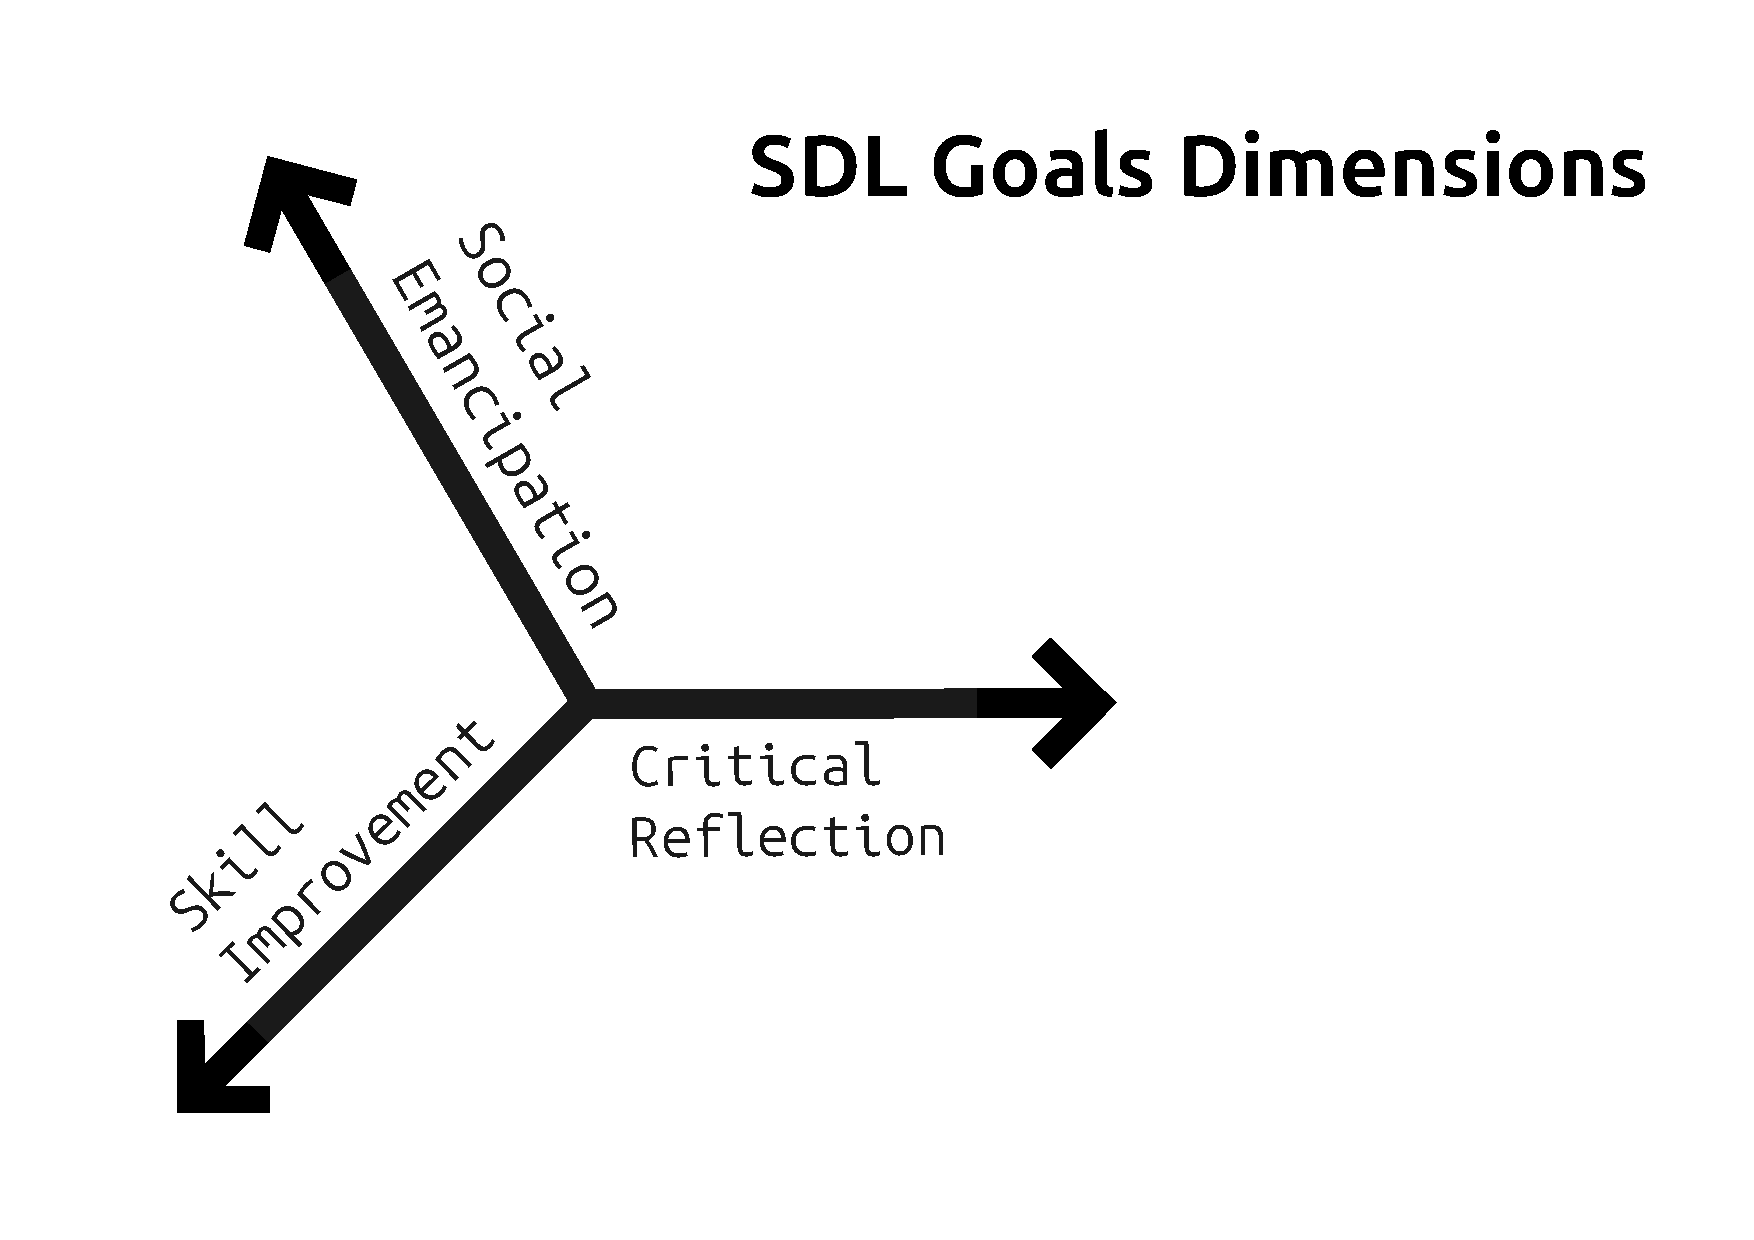
\includegraphics[width=0.9\textwidth]{images/chapter-02/sld-goals-3d.pdf}}

\par\medskip\ABNTEXfontereduzida\selectfont\textbf{Source:} Created by the author (2024).
%\citeauthor{manualufpe2020} (\citeyear{manualufpe2020}) \par\medskip
\end{figure}

\subsection{Skill Improvement}
\label{sdl-goal-ss:skill}

The first \gls{SDL} goal is closer to “a set of personal attributes and specific skills” \cite[p.~107]{merriam:2007}. This perspective appears to be coming out of a liberal education, providing, if necessary, an enhancement of personal attributes. The idea behind it is to prepare the student for planning, carrying out, and evaluating their own learning. 

However, there is no focus on changing consciousness, nor using this process as a means to emancipate the learner against an established and oppressive situation. Usually, this skill improvement of being a self-directed learner is given as a necessary formation step and one of the professional’s differentials in seeking better opportunities in the labor market\footnote{I prefer to use "job world" instead of "labor market". The underlying idea behind the "labor market" seems to consider human beings as available products to be sold. Thus, these products are called "human resources" and need to be attractive enough to fill the shelves of this "labor market" for organizations to consume them (similar to raw materials). "Job world", in my understanding, does not carry this range of meanings, expanding our view concerning jobs.}.

This goal is related to the expected stance of a liberal citizen in our society as a lifelong learner. Due to fast changes happening in our industrialized context, being the major part caused by the use of technology as a competitive differential, the citizens need to follow this flux and prepare themselves to adapt to a new situation constantly. This includes being ready to learn new competencies and, if necessary, to change their job drastically. In this way, a lifelong learner is not only a result of a new understanding of human development, admitting a biological possibility to learn even during adult life. A lifelong learner is necessary to support a liberal model of society proposed currently.

This perspective comprehends the major part of \gls{SDL} research. It is essential to highlight that this goal can assume humanistic traits related to responsibility and personal autonomy like free will to make individual choices, being more associated with accountability.

% \vspace{0.3cm}
% \fbox{
%     \begin{minipage}[htb]{0.9\textwidth}
%         \vspace{0.3cm}
                
%         \colorbox{gray!30}{% create a colored box
%             \makebox[0.975\textwidth][l]{% center the text on the page
%                 \ \ \textbf{Further Writing}
%             }
%         }

%         \vspace{0.1cm}
        
%         \begin{itemize}
%             \item Showing that this perspective comprehends the major part of SDL research.
%             \item Discussing why this goal can assume humanistic traits related to responsibility and personal autonomy (free will to make individual choices and more associated with accountability).

%         \end{itemize}

%         \vspace{0.25cm}
        
%     \end{minipage}
% }

\subsection{Critical Reflection}
\label{sdl-goal-ss:reflection}

The second \gls{SDL} goal is not only committed to skill improvement but also concerned with students' personal growth from this perspective. The crucial difference here is the source of students’ learning needs. From a skill improvement perspective, the first driving force that provokes their learning needs is extrinsic. The labor market, for example, establishes its demands previously and continuously, staving and shaping what should be necessary to compose a school curriculum and, only subsequently, allowing students to choose learning needs from a limited range of options.

This goal is closer to students' intrinsic motivation. Although there is an inward dimension to want learning, learning needs are socially determined and, for this reason, also naturally determined by different social actors, including the actors belonging to the so-called "labor market”. However, the weight of this impact matters and the contribution of other social actors need to be considered in this perspective.


From this lens, transformational learning \cite{boyer:2006,vallance:2016} proposes a similar epistemological framework. It is also important to point out that the lifelong learning \cite{shen:2020,kastelan:2023} can assume this perspective, providing these skills in response to the learner’s pursuit of their interests (like Maslow's theory of self-actualization \cite{compton:2024}).

% \vspace{0.3cm}
% \fbox{
%     \begin{minipage}[htb]{0.9\textwidth}
%         \vspace{0.3cm}
                
%         \colorbox{gray!30}{% create a colored box
%             \makebox[0.975\textwidth][l]{% center the text on the page
%                 \ \ \textbf{Further Writing}
%             }
%         }

%         \vspace{0.1cm}
        
%         \begin{itemize}
%             \item Developing the intrinsic motivation in this perspective.
%             \item Expliciting that learning needs are socially determined and, for this reason, naturally determined by different social actors, including the actors belonging to the so-called “labor market” But the weight of this impact matters and the contribution of other social actors need to be considered in this perspective.
%             \item Correlating to transformative learning.
%             \item Showing that lifelong learning can assume this perspective, providing these skills in response to the learner’s pursuit of their interests (Maslow).
%         \end{itemize}

%         \vspace{0.25cm}
        
%     \end{minipage}
% }

\subsection{Social Emancipation}
\label{sdl-goal-ss:emanc}

The last goal adopts an emancipatory learning stance including social action \cite{tissenbaum:2019}. Bearing in mind that it is impossible to be neutral in our pedagogical practice \cite{bispojr:2022-educomp}, this perspective gives a next step towards an education that commit itself against oppression. In "The Pedagogy of Oppressed", \citeonline[p.~44]{freire:2000-oppressed} identifies the oppressor-oppressed binomial, having as its main marks the dehumanization process. For him, the human beings' search for a fulfilled life lead to overcome this contradiction, rehumanizing both oppressor and oppressed through a proposal of a new relation between them that can be achieved by means of an emancipatory education. From this lens, \gls{SDL} is an activity strongly relational, because "the liberation of the oppressed is a liberation of women and men, not things. [...] [N]o one liberates himself by his own efforts alone, neither is he liberated by others" \cite[p.~66]{freire:2000-oppressed}.

In this goal, \citeonline[p.~227]{brookfield:1993} exposed a new way to understanding self-direction, considering it "as part of a cultural tradition that emphasizes the individual's standing against repressive interests". He pointed out two political dimensions of self-direction: control and access to resources. Concerning control, he asserted that:
\begin{citacao}
    "The one consistent element in the majority of definitions of self-direction is the importance of the learner's exercising control over all educational decisions. [...] This emphasis on control - on who decides what is right and good and how these things should be pursued - is also central to notions of emancipatory adult education" \cite[p.~233]{brookfield:1993}.
\end{citacao}
And, concerning access to resources, he explained the following:
\begin{citacao}
    "The full meaning of control in a self-directed learning project cannot be realized simply by wishing it into existence. [...] Being self-directed is a meaningless idea if you are too weary at the end of the day to think clearly about what form of learning would be of most use to you, or if you are closed off from access to the resources necessary for you to be able to realize your self-designed projects" \cite[p.~237]{brookfield:1993}.
\end{citacao}
Thus, he reveals the interconnections between \gls{SDL} and equity discussions (explored more in Chapter \ref{chap:equity}).

% \fbox{
%     \begin{minipage}[htb]{0.9\textwidth}
%         \vspace{0.3cm}
                
%         \colorbox{gray!30}{% create a colored box
%             \makebox[0.975\textwidth][l]{% center the text on the page
%                 \ \ \textbf{Further Writing}
%             }
%         }

%         \vspace{0.1cm}
        
%         \begin{itemize}
%             \item Presenting SDL as a means to promote emancipation.
%             \item Pointing to some considerations listed by Brookfield (1993) about equity issues and SDL.
%             \item Indicating the possibility of viewing SDL as a process through a model (link to next section).
%         \end{itemize}

%         \vspace{0.25cm}
        
%     \end{minipage}
% }


\section{SDL Models}
\label{sdl-sec:models}

Bearing that Knowles’ definition of \gls{SDL} occupies a prominent position in literature, it is usual to see \gls{SDL} as a process. Thus, different proposed models represent the understanding of the \gls{SDL} process and its constituent parts. \citeauthoronline{merriam:2007} (\citeyear{merriam:2007}, p.~110) classify these models into three types: linear, interactive, and instructional. For the \gls{Ph.D.} research purposes, I will present in more detail the linear (Section \ref{sdl-models-ss:linear}) and instructional (Section \ref{sdl-models-ss:instructional}) ones. The model type indicates how a pedagogical approach can embody the \gls{SDL} goals.

\subsection{Linear Models}
\label{sdl-models-ss:linear}

The first proposed models to \gls{SDL} had this characteristic: linearity. It is possible that the early authors did not believe strictly in this way. But, due to the inexistence of previous references, I think it is natural to propose a first minimum scaffold to refine it in the future. In this way, it does not seem to me as a helpful comprehension that these authors are “naive” when they propose their models. They give the first steps towards a better understanding and deepening \gls{SDL} as a process.

I list two prominent representatives of linear models: Allen Tough and Malcolm Knowles. I will discuss Knowles’ description of \gls{SDL} as a process in more detail. From Knowles' definition and my schema presented in Figure \ref{fig:sdl-process}, it is possible to identify five phases: (i) diagnosing learning needs, (ii) formulating learning goals, (iii) identifying human and material resources for learning, (iv) choosing and implementing appropriate learning strategies, and (iv) evaluating learning outcomes. Although it is not present in the literal definition, Knowles (\citeyear{knowles:1975}, p.~9, 29, 60) also adopts a preliminary phase called “setting a climate”. Thus, it is possible to see Knowles' model as composed of six phases instead of five.

We can compare the \gls{SDL} linear models to the first software lifecycle models. The waterfall model \cite[p.~8]{ruparelia:2010} also proposes a well-established sequence of phases that may invoke feedback loops. I believe that both Tough and Knowles considered other variables like internal dispositions or social context of the learner and judged them necessary during the \gls{SDL} process. However, these variables were not explicitly expressed in their proposed models. I list in Table \ref{tbl:sdl-competencies} all competencies proposed by Knowles (\citeyear{knowles:1975}, p.~61) to be used by self-directed learners as a self-rating instrument.

\begin{table}[ht]
\caption{List of \acrshort{SDL} competencies proposed for a self-rating instrument.}
\label{tbl:sdl-competencies}
\centering
\rowcolors{1}{}{lightgray}
\begin{tabular}{p{0.5cm}p{14.5cm}}
\hline
\multicolumn{2}{c}{\textbf{Competencies of Self-Directed Learning}} \\
\hline     
1 &
An understanding of the differences in assumptions about learners and the skills required for learning under teacher-directed learning and self-directed learning, and the ability to explain these differences to others.\\
2 &
A concept of myself as being a non-dependent and a self-directing person.\\
3 &
The ability to relate to peers collaboratively, to see them as resources for diagnosing needs, planning my learning, and learning; and to give help to them and receive help from them.\\
4 &
The ability to diagnose my own learning needs realistically, with help from teachers and peers.\\
5 &
The ability to translate learning needs into learning objectives in a form that makes it possible for their accomplishment to be assessed.\\
6 &
The ability to relate to teachers as facilitators, helpers, or consultants, and to take the initiative in making use of their resources.\\
7 &
The ability to identify human and material resources appropriate to different kinds of learning objectives.\\
8 &
The ability to select effective strategies for making use of learning resources and to perform these strategies skillfully and with initiative.\\
9 &
The ability to collect and validate evidence of the accomplishment of various kinds of learning objectives.\\
\hline

\end{tabular}

  \par\medskip\ABNTEXfontereduzida\selectfont\textbf{Source:} Adapted from \cite[p.~61]{knowles:1975}. \par\medskip
\end{table}

There are two main critiques of this type of model. First, the linearity can lead the learner or facilitator to admit this sequence as a strict and irrevocable flux to follow, precluding necessary returns to early phases to guarantee effective learning. Second, the simplicity of these models does not explicitly address other internal dimensions of the learner beyond the cognitive or meta-cognitive aspects (e.g., feelings) or external dimensions like structural barriers (e.g., racism, poverty). 

% \subsection{Interactive Models}
% \label{sdl-models-ss:interactive}

% \fbox{
%     \begin{minipage}[htb]{0.9\textwidth}
%         \vspace{0.3cm}
                
%         \colorbox{gray!30}{% create a colored box
%             \makebox[0.975\textrefers][l]{% center the text on the page
%                 \ \ \textbf{Further Writing}
%             }
%         }

%         \vspace{0.1cm}
        
%         \begin{itemize}
%             \item Presenting the main characteristics of interactive models.
%             \item Pointing out their limitations.

%         \end{itemize}

%         \vspace{0.25cm}
        
%     \end{minipage}
% }


\subsection{Instructional Models}
\label{sdl-models-ss:instructional}

The last class of \gls{SDL} models refers to frameworks that teachers can utilize in order to foster \gls{SDL} competencies into their programs and activities. I will present the \gls{SSDL} Model that “suggests how teachers can actively equip students to become more self-directed in their learning” \cite[p.~126]{grow:1991}. To achieve this, an axis (ranging from an Authority/Coach to a Consultant /Delegator teacher) situates what standing should be adopted in each situation (Table \ref{tbl:ssdl-model}).

% \fbox{
%     \begin{minipage}[htb]{0.9\textwidth}
%         \vspace{0.3cm}
                
%         \colorbox{gray!30}{% create a colored box
%             \makebox[0.975\textwidth][l]{% center the text on the page
%                 \ \ \textbf{Further Writing}
%             }
%         }

%         \vspace{0.1cm}
        
%         \begin{itemize}
%             \item Presenting the main characteristics of instructional models.
%             \item Describing in more detail the \gls{SSDL} Model (Table \ref{tbl:ssdl-model}) that “suggests how teachers can actively equip students to become more self-directed in their learning” \cite[p.~126]{grow:1991}.
%             \item Scrutinizing both the teacher and students’ stages (Figure \ref{fig:ssdl-matrix}).
%             \item Indicating that this work uses a combination of \citeauthoronline{knowles:1975}’ and \citeauthoronline{grow:1991}'s models.
%             \item Linking to the next section (challenges in \gls{SDL}).
%             \item Listing some limitations.

%         \end{itemize}

%         \vspace{0.25cm}
        
%     \end{minipage}
% }

\begin{table}[ht]
\caption{Staged \acrshort{SDL} Model structured into a table.}
\label{tbl:ssdl-model}
\centering
\rowcolors{1}{}{lightgray}
\begin{tabular}{
    >{\centering\arraybackslash}p{1.5cm}
    >{\centering\arraybackslash}p{3cm}
    >{\centering\arraybackslash}p{2cm}
    p{5.5cm}
}
\hline
\multicolumn{1}{c}{
    \textbf{Stage}
} &
\multicolumn{1}{c}{
    \textbf{Student}
} &
\multicolumn{1}{c}{
    \textbf{Teacher}
} &
\multicolumn{1}{c}{
    \textbf{Examples}
} \\
\hline     
Stage 1 &
Dependent &
Authority Coach &
Coaching with immediate feedback. Drill. Informational lecture. Overcoming deficiencies and resistance.\\
Stage 2 &
Interested &
Motivator, guide &
Inspiring lecture plus guided discussion. Goal-setting and learning strategies.\\
Stage 3 &
Involved &
Facilitator &
Discussion facilitated by teacher who participates as equal. Seminar. Group projects.\\
Stage 4 &
Self-directed &
Consultant, delegator &
Internship, dissertation, individual work or self-directed study-group.\\
\hline

\end{tabular}

  \par\medskip\ABNTEXfontereduzida\selectfont\textbf{Source:} Adapted from \cite{grow:1991}. \par\medskip
\end{table}

\citeauthoronline{grow:1991}'s model also signals how would be a desirable matching between student \gls{SDL} stage and teacher standing. Figure \ref{fig:ssdl-matrix} shows a confusion matrix, highlighting that it should exist a dynamic in our educational practices aiming to materialize \gls{SDL} of our students. In this research, I adopt a combination of \citeauthoronline{knowles:1975}’ and \citeauthoronline{grow:1991}'s models, providing the constructs for the discussion of results.

\begin{figure}[ht!]
\centering

\caption{\textmd{Staged \acrshort{SDL} Model structured from a confusion matrix.}}
\label{fig:ssdl-matrix}
\fcolorbox{gray}{white}{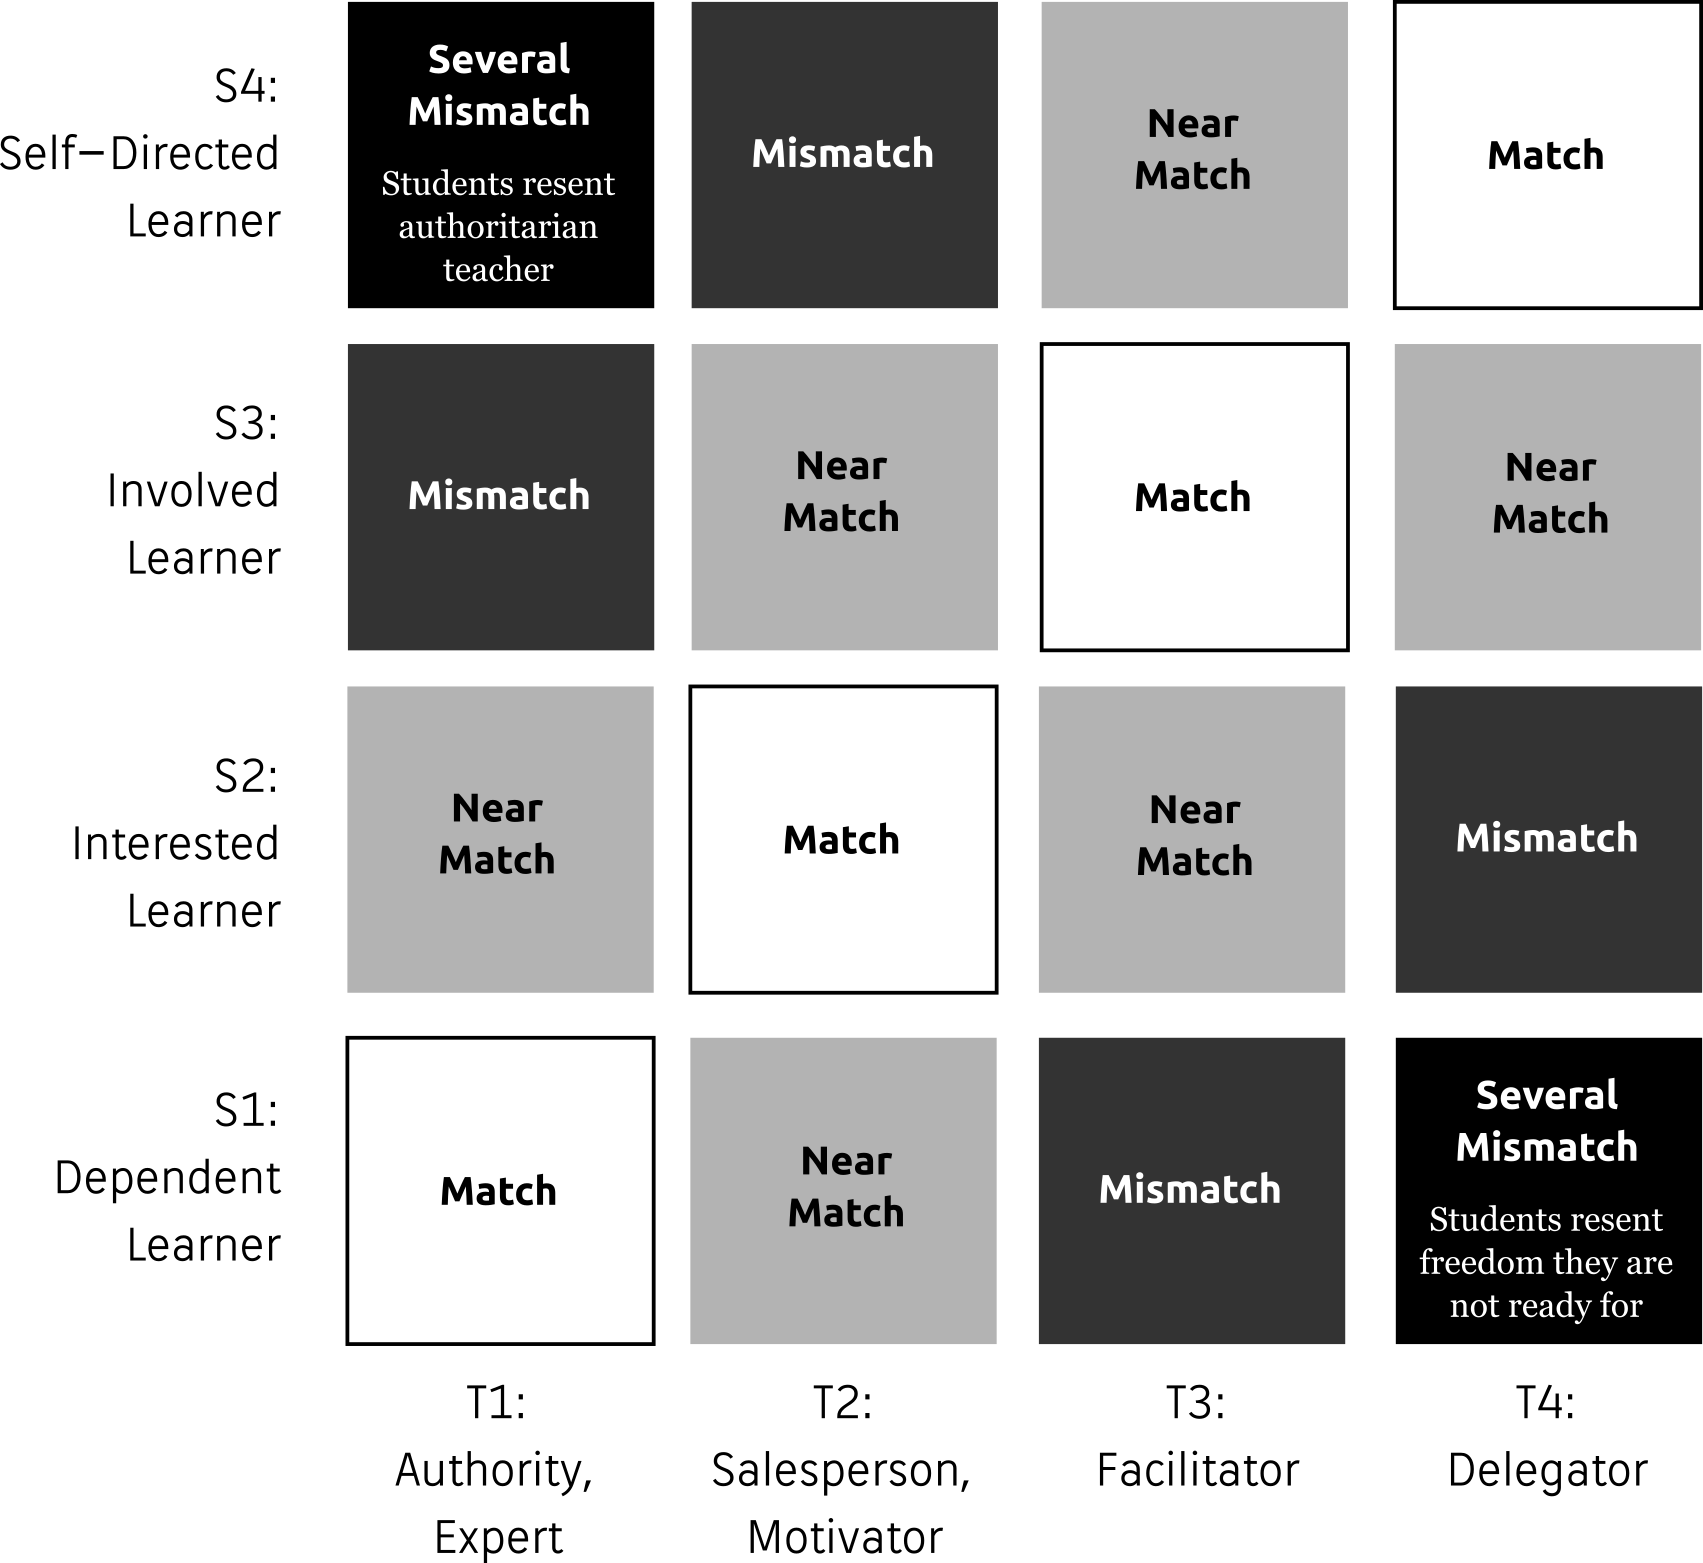
\includegraphics[width=0.9\textwidth]{images/chapter-02/grow.png}}

\par\medskip\ABNTEXfontereduzida\selectfont\textbf{Source:} Adapted from \cite{grow:1991}.%\citeauthor{manualufpe2020} (\citeyear{manualufpe2020}) \par\medskip
\end{figure}
\section{Some SDL Relations}
\label{sdl-sec:relations}

Researching \gls{SDL} is strategic due to several relations with other educational concepts and perspectives. This section presents relations from \gls{SDL} to learning in adulthood (Section \ref{sdl-relations-ss:andragogy}), problem-based learning (Section \ref{sdl-relations-ss:pbl}), and self-regulated learning (Section \ref{sdl-relations-ss:srl}).

\subsection{SDL and Learning in Adulthood}
\label{sdl-relations-ss:andragogy}

In the major part of the 20th century,  learning in adulthood was considered a synonym for adult education. Bearing in mind that the understanding of what adulthood is and what an adult can do and be has changed over time (e.g., the conception about the emerging adulthood \cite{parameswaran:2020}), learning in adulthood is an organic area that has been evolving continuously. Currently, learning in adulthood encompasses many learning situations (e.g., professional, personal learning needs) and learning spaces (e.g., formal, nonformal, informal learning), revealing that adult education is one of the various possibilities to address the phenomenon. Aiming to illustrate the rich relations between \gls{SDL} and learning in adulthood, I will focus on Knowles' andragogy and Freire's pedagogy of the oppressed.

Knowles' andragogy \cite{knowles:2005} is based on the need to understand how adults learn differently than children. Andragogy usually rests on six assumptions involving epistemological and anthropological perspectives about the adult and their learning. One of these assumptions is that an adult would tend to a self-direction stance instead of a more dependent one \cite[p.~84]{merriam:2007}. This self-direction propensity would conduct adult to  \gls{SDL} naturally. Thus, teaching adults considering their current human development stage and phase of social life requires adopting pedagogical perspectives toward \gls{SDL}.

Freire's pedagogy of the oppressed \cite{freire:2000-oppressed} arose from a different context of andragogy, rooted in poverty, illiteracy, and oppression among adults. Freire does not differentiate personal empowerment and social transformation, enabling the adult learner "to speak a true work" and "transform the world" simultaneously \cite[p.~87]{freire:2000-oppressed}. This pedagogy becomes concrete through a robust dialogic process, giving up from authoritarian perspectives (called by him "banking education") to a collective and situated construction of both curricula and learning. Thus, inside Freire's pedagogy, \gls{SDL} always appears as a means to promoting critical reflection, putting all stages of Knowles' \gls{SDL} in a sociocultural pedagogical action, reframing the classical notion of an individual adult learner. \citeonline{owen:2002} puts Freire's \gls{SDL} in adulthood learning beside Jack Merirow and Stephen Brookfield as critical perspectives.

\subsection{SDL in Problem-Based Learning}
\label{sdl-relations-ss:pbl}

\gls{SDL} plays a crucial role in the \gls{PBL} approach. \citeauthoronline{savery:1995} (\citeyear{savery:1995}, p.~4) define \gls{PBL} as "a general model [that uses] authentic problems as the stimulus for and organizer of learning activities and the learners work in small collaborative groups". \gls{PBL} has been adopted in Computing Education for a long time \cite{santos:2021}, and there are multiple paths to incorporate it from a single course scope to an entire program curriculum.

Aiming to assess the \gls{PBL} approach, \citeauthoronline{savery:1995} assert that it should have "both a critique of performance and suggestions of ways to improve in three areas: self directed learning; problem solving; skills as a group member". Thus, it is possible to realize that, for them, \gls{SDL} is one of the three essential areas when we adopt \gls{PBL}.

Another way to realize the importance of \gls{SDL} in \gls{PBL} is by analyzing the \gls{PBL} principles. Santos and colleagues \cite{santos:2013,santos:2014,santos:2016,arruda:2019} extracted ten principles of the \gls{PBL} approach from the main \gls{PBL} literature, including the seminal papers of \citeauthoronline{savery:1995}. These ten \gls{PBL} principles are listed in Table \ref{tbl:pbl-principles}. Of ten principles, five are strongly related to \gls{SDL} (Principles 2, 5, 7, 8, and 9). Hence, this evidences how \gls{SDL} is fundamental in the \gls{PBL} conception.

\begin{table}[ht]
\caption{Ten \acrshort{PBL} principles and their relation to \gls{SDL}.}
\label{tbl:pbl-principles}
\centering
\rowcolors{1}{}{lightgray}
\begin{tabular}{
    >{\centering\arraybackslash}p{1cm}
    p{9.7cm}
    >{\centering\arraybackslash}p{3.5cm}
}
\hline
\multicolumn{1}{c}{
    \textbf{\#}
} &
\multicolumn{1}{c}{
    \textbf{Principle}
} &
\multicolumn{1}{c}{
    \textbf{Relation to SDL}
} \\
\hline     
1 &
Problem(s) at the core of the educational proposal. &
-\\
2 &
Learner as the owner of the problem. &
Strong\\
3 &
Authenticity of the problem or task. &
-\\
4 &
Authenticity of the learning environment. &
-\\
5 &
Learner drives the problem-solving process. &
Strong\\
6 &
Complexity of the problem or task. &
-\\
7 &
Learners test ideas against alternative views and contexts. &
Strong\\
8 &
Reflection on the content and process learned.&
Strong \\
9 &
Collaboration and multidirectional learning. &
Strong\\
10 &
Continuous assessment. &
-\\
\hline

\end{tabular}

  \par\medskip\ABNTEXfontereduzida\selectfont\textbf{Source:} \citeonline{santos:2014}. \par\medskip
\end{table}

Other relations can be identified between \gls{SDL} and \gls{PBL}. \citeonline[p.~193]{leary:2019} presented evidence supporting some claims that
\begin{citacao}
    "[...] PBL promotes self-directed learning both as a process within PBL and as an outcome of effective PBL interventions. Further, self-directed learning is mediated heavily by student and teacher perceptions, by environmental factors, and by underlying models that are used (or not) as part of a larger intervention".
\end{citacao}
The authors also mention the benefit of \gls{SDL} development in the \gls{PBL} process:
\begin{citacao}
    "The development of effective self-directed learning skills includes self-assess\-ment and flexible knowledge so that the student understands their personal learning needs and where to find and use appropriate information for problem-solving. [...] They need to set goals and be able to identify their knowledge gaps, strategize how to reach their goals, implement the plan, and assess if they have reached their goal. The collaborative part of self-directed learning encompasses all aspects of working in a group and, as students commence work in PBL environments, working through problems they build their self-directed learning skills" \cite[p.~188]{leary:2019}.
\end{citacao}
Lastly, \citeonline[p.~183]{leary:2019} show the difference between \gls{SDL} and self-regulated learning but attest to the similarity between them in \gls{PBL} contexts:
\begin{citacao}
    "Self-regulated learning focuses on narrow micro-level constructs with tasks typically set by a teacher in a formal learning environment, while self-directed learning stems from adult education and involves broader macro-level constructs initiated by students. Zimmerman and Lebeau contend that in context of PBL, that self-regulated learning and self-directed learning are highly similar and oftentimes the literature uses the terms interchangeably".
\end{citacao}


\subsection{SDL and Self-Regulated Learning}
\label{sdl-relations-ss:srl}

\gls{SRL} is "an active, constructive process whereby learners set goals for their learning and then attempt to monitor, regulate, and control their cognition, motivation, and behavior, guided and constrained by their goals and the contextual features in the environment" \cite[p.~453]{pintrich:2000}. As mentioned in the previous section, \gls{SRL} has an interchangeable use to \gls{SDL} in \gls{PBL} context, but, although its definition closely relates to \gls{SDL} one, there are differences between them.

\citeonline[p.~192]{saks:2014} present a list of differences between these two concepts ranging from (i) origins, (ii) kind of educational space, and (iii) construct level. \gls{SDL} came from Adult Education, while \gls{SRL} came from Educational and Cognitive Psychology. \gls{SDL} is most used to describe activities outside the traditional school environment, while \gls{SRL} is more studied in formal spaces. \gls{SDL} involves a broader macro-level construct initiated by students, while \gls{SRL} focuses on narrow micro-level constructs.

The relation between them is better described by \cite[p.~192]{saks:2014}:
\begin{citacao}
    "Self-directed learning has been considered a broader construct encompassing self-regulated learning as narrower and more specific one. SDL has also been treated as a broader concept in the sense of learner's freedom to manage his learning activities and the degree of control the learner has. In SDL this is the learner who defines the learning task, in SRL it may also be a teacher. [...] Self-directed learning may include self-regulated learning but not the opposite. In other words, a self-directed learner is supposed to self-regulate, but a self-regulated learner may not self-direct. From this point of view, self-directed learning deals more with subsequent steps in the learning process. Providing students with opportunities for self-directed practice can help to improve their self-regulation".
\end{citacao}
\citeonline[p.~418]{loyens:2008} go at same direction concerning the \gls{SDL} coverage:
\begin{citacao}
    "In sum, the concept of SDL is broader than SRL. SDL as a design feature of the learning environment stresses students' freedom in the pursuit of their learning. 
    
    [...] As such, a closer examination of both SRL and SDL as learning processes brings the issue of student control over the learning task to the fore. Clearly, both SDL and SRL carry an element of student control. However, the degree of control the learner has, specifically at the beginning of the learning process when the learning task is defined, differs in SDL and SRL. In SDL, the learning task is always defined by the learner. A self-directed learner should be able to define what needs to be learned. [...] In this sense, SDL can encompass SRL, but the opposite does not hold. SRL seems more concerned with the subsequent steps in the learning process such as learning goals and strategies, while SDL clearly provides a crucial role for the learner at the outset of the learning task".
\end{citacao}
\section{Some Research Challenges and Opportunities}
\label{sdl-sec:challenges}

\citeonline[p.~128]{merriam:2007} listed some challenges in \gls{SDL} research, posing these questions bearing in mind adult education mainly. I highlight three of them:
\begin{itemize}
    \item[(i)] "Are there public policy issues at the national, state, or local level related to \gls{SDL}? If so, what roles could adult educators play in advocating and developing such policies?
    \item[(ii)] To what extent is \gls{SDL} situational or cultural?
    \item[(iii)] How do cultural and contextual factors shape \gls{SDL}?”
\end{itemize}
This \gls{Ph.D.} thesis, when addressing equity issues in a developing country context, aims to explore better these three questions in a \gls{CSE} scenario.

Several studies addressed the meeting between \gls{SDL} and \gls{CEd}, signaling good promissory ways of researching this topic. \citeonline{mccartney:2016} investigated the reasons computing students learn on their own, interviewing seventeen students from different backgrounds. \citeonline{tagare:2023} reviewed the literature looking for the dispositions that computing professionals value, identifying two of five themes strongly related to \gls{SDL} (self-regulation and lifelong orientation). \citeonline{cawley:2014} incorporated what they called \gls{SDL} pedagogy in computing classroom in \gls{PBL} software engineering courses. Lastly, \citeonline{maphalala:2024} faced \gls{CSE} under the \gls{SDL} lens, reviewing existing research in this area.
  
\chapter{Equity}
\label{chap:equity}

 One of the emerging challenges in \acrfull{CEd} refers to diversity \cite[p.~19:2]{burgstahler:2011}. Existing differences in a classroom can be a source of wealth and beauty. But they can also be a source of tensions that can generate conflicts. These conflicts are directly associated with the existence of privilege deriving from these differences.
 
According to \citeonline[p.~1]{parker:2015}, privilege is “an unearned, unasked-for advantage gained because of the way society views an aspect of a student’s identity, such as race, ethnicity, gender, socioeconomic status, and language”. The \gls{IBGE}\footnote{IBGE stands for \textit{Instituto Brasileiro de Geografia e Estatística} in Brazilian Portuguese.} conducted the \gls{PNAD Contínua}\footnote{PNAD Contínua stands for \textit{Pesquisa Nacional por Amostra de Domicílios Contínua} in Brazilian Portuguese.} in 2018, relating the theme of Information and Communication Technology. This survey revealed that one in four Brazilian people does not have internet access. Suppose we admit that a fraction of these Brazilians who do not have internet access were composed of students in an undergraduate computing program. What would be the impact of this reality on their education quality? What would be the difference in the education quality of these students relating to others? Scenarios like this show that the differences can convert in privilege to a specific social stratum of the scholar community.

The understanding that there is inequality in the conditions of student's context is fundamental for promoting social justice in \acrfull{CSE}. This perception allows the professor to reorganize their priorities and build a more honest frame of emerging problems deriving from the diversity of their scholar community.

Some concepts are essential when we refer to inequality of opportunities in education. \citeonline[p.~482]{lewis:2019} assert that:
\begin{citacao}
    “\textit{Equality} refers to the state where everyone has or is allocated the same things in the same degree, whereas \textit{equity} typically refers to having access to what is needed. [...] In general, [...] equity, and not equality, defines fair and just learning opportunities” (my emphasis).
\end{citacao}
An exciting way to understand the two concepts is by employing an illustration\footnote{Angus Maguire created this illustration and made it available in his portfolio: \url{http://madewithangus.com/portfolio/equality-vs-equity/.}} (Figure \ref{fig:equality-vs-equity}). The equality of conditions does not necessarily guarantee the real equality of opportunities. If we want everybody to have a real chance to watch the match, there must be a differentiated and intentional treatment. 

\begin{figure}[ht!]
\centering

\caption{\textmd{Illustration about the difference between equality and equity.}}
\label{fig:equality-vs-equity}
\fcolorbox{gray}{white}{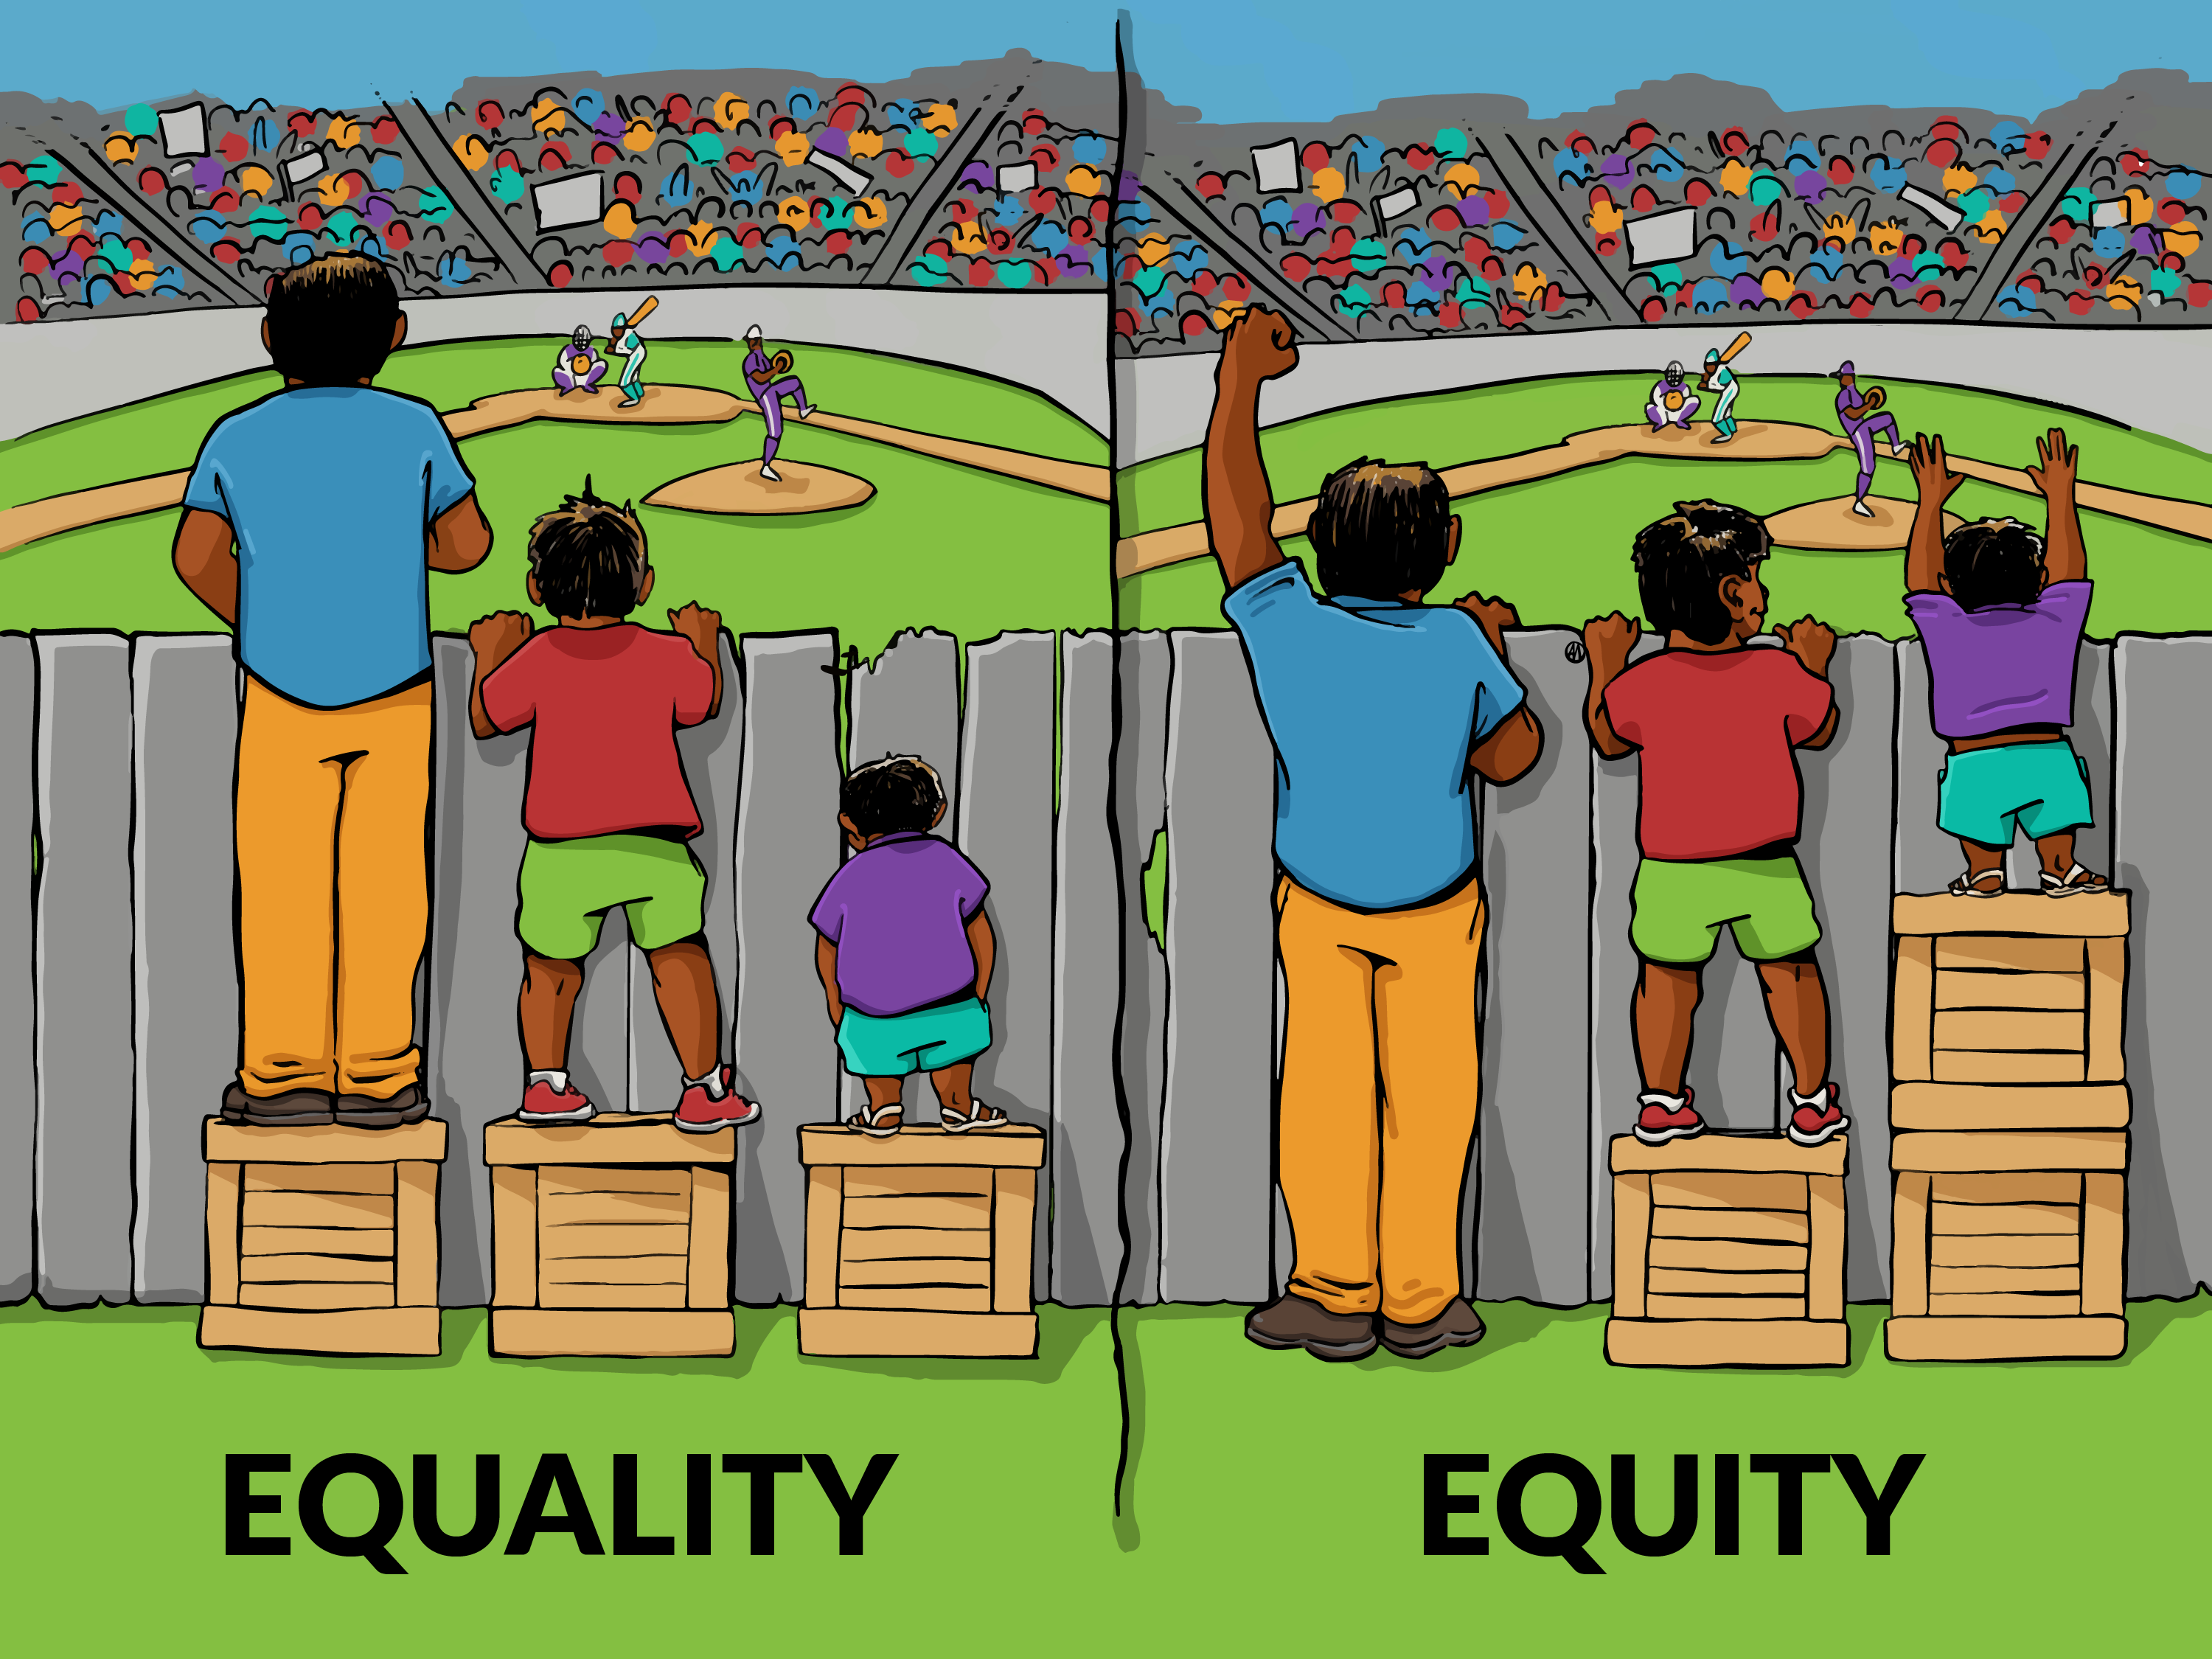
\includegraphics[width=0.7\textwidth]{images/chapter-03/equality-vs-equity.png}}

\par\medskip\ABNTEXfontereduzida\selectfont\textbf{Source:} Created by Angus Maguire \cite{maguire:2016}.%\citeauthor{manualufpe2020} (\citeyear{manualufpe2020}) \par\medskip
\end{figure}

Throughout this chapter, I detail the consequences of admitting this differentiated treatment to promote social justice in \gls{CSE}. Section \ref{equity-sec:diff-prin} shows the difference principle proposed by John Rawls. Section \ref{equity-sec:sen-ca} explains the capability approach of Amartya Sen and what it advances in the discussion about equity. Section \ref{equity-sec:cape} details the \gls{CAPE} framework, eliciting its elements, and how it has been used to analyze \gls{CSE} equity issues. Section \ref{equity-sec:br-context} describes the Brazilian context concerning the adoption of affirmative actions in higher education. And, at last, Section \ref{equity-sec:active-learning} points out the emergent issues when we investigate equity in active methodologies in \gls{CEd}.

\section{Rawls: Difference Principle}
\label{equity-sec:diff-prin}

Still developing the distinction between equality and equity, I present the difference principle stated by \citeonline{rawls:1971}. Rawls was a \gls{USA} citizen and political philosopher in the liberal tradition \cite{wenar:2021}. His theory structures a society under the lens of an egalitarian economic system.

Hans Traxler\footnote{It is known that Hans Traxler, a Czech illustrator, created the original cartoon in 1976 \cite{traxler:2019}. But it is unknown the artist who translated it for English version. See more details \url{https://historyof.place/the-politics-of-disability-from-6th-century-china-to-the-industrial-revolution/}.} created an excellent illustration (Figure \ref{fig:fair-selection-traxler}) that helps us to delve into this discussion. In the first moment, it is natural to assume that equal treatment is a synonym for justice. But there are several scenarios, like that presented by Traxler, evidencing the issues that can emerge for our students from this premise. 

\begin{figure}[ht!]
\centering

\caption{\textmd{Illustration translated from original cartoon created by Hans Traxler.}}
\label{fig:fair-selection-traxler}
\fcolorbox{gray}{white}{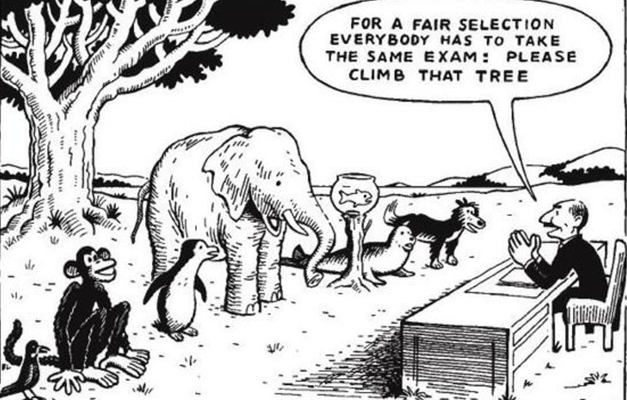
\includegraphics[width=0.8\textwidth]{images/chapter-03/traxler-illustration.jpg}}

\par\medskip\ABNTEXfontereduzida\selectfont\textbf{Source:} Created by Traxler \cite{traxler:2019}.%\citeauthor{manualufpe2020} (\citeyear{manualufpe2020}) \par\medskip
\end{figure}

The crucial point here is that, probably, the underlying reason to apply equal treatment to foster social justice is our search for equality of opportunities. Equal treatment used to be the default solution to tackle common justice problems in our day-to-day life. But equal treatment is not what we are searching for. We use equal treatment aiming for equality of opportunities. In this way, it will be necessary to discern when to make use of equal treatment or not. Just in this point Rawls' principle plays an essential role in the discussion about equality and equity.

Rawls' starting point is what he called the “original position” for all people of an imaginary society that does not exist yet. \citeauthoronline{rawls:1971} (\citeyear{rawls:1971}, p.~12) develops this idea clearly, asserting that:
\begin{citacao}
    “[N]o one knows his place in society, his class position or social status, nor does anyone know his fortune in the distribution of natural assets and abilities, his intelligence, strength, and the like. I shall even assume that the parties do not know their conceptions of the good or their special psychological propensities. The principles of justice are chosen behind a veil of ignorance”.    
\end{citacao}

And what are these principles? \citeauthoronline{rawls:1971} (\citeyear{rawls:1971}, p.~83) lists two that would naturally arise from the veil of ignorance. The second principle states the following:
\begin{citacao}
    “2. Social and economic inequalities are to be arranged so that they are both:
    
    \hspace{0.5cm} (a) to the greatest benefit of the least advantaged, consistent with the just savings principle, and
    
    \hspace{0.5cm} (b) attached to offices and positions open to all under conditions of fair equality of opportunity".
\end{citacao}
 
Part (a) of this principle is what Rawls named the difference principle. The difference principle is a rational justification for a differentiated treatment aiming to promote equality of opportunities.

Why more boxes for the child (Figure \ref{fig:equality-vs-equity})? Because we want to promote equality of opportunities. Thus, we guarantee the greatest benefit to the least advantaged originally. Why can we not apply the same exam for all (Figura \ref{fig:fair-selection-traxler})? Because we would not guarantee equality of opportunities for everybody. It is possible to connect this to what \citeauthoronline{parker:2015} (\citeyear{parker:2015}, p.~4) assert about the difference principle:
\begin{citacao}
    “[Strict] equality is privilege agnostic and implies giving every student equal opportunities no matter where they start. Justice is privilege sensitive and involves giving some students more opportunities than others based on how disadvantaged the student might be”.
\end{citacao}
Fostering privilege sensitivity matters if we want to build a school environment that does not reproduce the pre-existing inequalities in our society. Restructuring the school in an equitable direction signals an achievable changing perspective for society in seeking a fairer world.

Although the difference principle occupies a prominent position concerning equity discussion, the whole Rawls' theory of justice doesn't have the same acknowledgment. Many researchers (like me) are not interested in establishing a foundational theory (bearing in mind that Rawls' original position is only relevant to establishing a public reason in a collective debate). The reality is that it is not possible to reinitialize the whole society from this justice perspective. One more interesting proposal can be to identify and highlight the main aspects to consider to discuss equity appropriately (including by using the difference principle). \citeonline[p.~94]{robeyns:2005} presents the \acrfull{CA} as a possibility to address these questions in a framework perspective:
\begin{citacao}
    “Note that the capability approach is not a theory can explain poverty, inequality or well-being; instead, it rather provides a tool and a framework within which to conceptualize and evaluate these phenomena. Applying the capability approach to issues of policy and social change will therefore often require the addition of explanatory theories”.
\end{citacao}
Thus, I will present \gls{CA} in the next section from the perspective of an equity 
 conceptual framework.
        

\section{Sen: Capabilities Approach}
\label{equity-sec:sen-ca}

Following the discussion, the \glsfirst{CA} was proposed by Amartya Sen and puts the focus on other aspects when analyzing equity issues. Sen is an Indian economist and philosopher who follows the liberal tradition (like Rawls). He is known for his contributions to the creation of the \gls{HDI} \cite{bomfim:2012} and for winning the Nobel Prize \cite{nobel:2022}.

The main question raised by \citeonline[p.~12]{sen:1992} is "equality of what?". Sen's' concerns concentrated on the higher risk of reducing the efforts to deal with inequalities to a single-dimensional analysis. The inequality problem is complex and multidimensional by nature. Thus, when we analyze the problem only with the incoming inequality lens, for instance, other sources of inequalities can probably be neglected and, in some cases, even aggravated. Although the race lens, for example, can contribute to informing essential aspects that can not be overlooked by all stakeholders responsible for analyzing a given scenario, this one is not enough to inform a decision-maker with quality and robustness if isolated from others.

The unifier key point for Sen is the freedom to achieve well-being. Well-being is an issue of primary moral importance in Sen's' perspective. The well-being prism is the umbrella that allows for a more diverse analysis from different sources of inequities to dialog to achieve a single (but complex) commitment. In summary, the first normative claim of the theoretical framework of the \gls{CA} is that the freedom to achieve well-being is of primary moral importance. \citeonline[p.~3]{dreze:2002} explore this direction, asserting that:
\begin{citacao}
    "It should be clear that we have tended to judge development by the expansion of substantive freedoms - not just by the economic growth (for example, of the gross national product), or technical progress, or social modernization. This is not to deny, in any way, that advances in the latter fields can be very important, depending on circumstances, as ''instruments'' for the enhancement of human freedom. But they have to be appraised precisely in that light - in terms of their actual effectiveness in enriching the lives and liberties of people - rather than taking them to be valuable in themselves".
\end{citacao}

The second \gls{CA} claim is that the understanding of well-being is directly related to people's capabilities and functionings. When Sen attaches the proper comprehension of well-being to the concepts of functioning (Section \ref{sen-ss:functioning}) and capability (Section \ref{sen-ss:capability}), he shifts the concern to defining what well-being is exactly, exploring these two crucial \gls{CA} concepts in more detail. Honestly, Sen's contribution resides primarily in this shifting, indicating the primacy of well-being but does not exhaust it. Sen allows a certain plasticity level of his approach not to define well-being categorically. However, he establishes three concepts for guiding the discernment of dealing with an analysis from a multidimensional inequity perspective. Beyond functionings and capabilities, conversion factors (Section \ref{sen-ss:conv-fac}) are the third essential \gls{CA} concept.

\subsection{Functioning}
\label{sen-ss:functioning}

As mentioned, Sen does not define well-being but characterizes it in terms of functionings and capabilities. About functionings, he asserts that:
\begin{citacao}
    "The well-being of a person can be seen in terms of the quality of the person's being. Living may be seen as consisting of a set of interrelated ''functionings'', consisting of beings and doings. A person's' achievement in this respect can be seen as the vector of his or her functionings. The relevant functionings can vary from such elementary things as being adequately nourished, being in good health, avoiding escapable morbidity and premature mortality, etc., to more complex achievements such as being happy, having self-respect, taking part in the life of the community, and so on" \cite[p.~39]{sen:1992}.
\end{citacao}
Thus, functionings are beings and doings that are "various states of human beings and activities that a person has achieved" \cite{robeyns:2023}.

From an educational perspective, I can exemplify this concept from a political-pedagogical project of a computing program. When a professor's group delineates a graduate profile, it idealizes all the expected functionings that a student should achieve after the completion of the course. In this way, beings like "to be proactive" or "able to work in groups", and doings like "sorting an array" and "modeling a database" are functioning descriptions. All these would be relevant functionings that a graduate should have. Thus, there is a vector of interrelated functionings that describes a graduate profile appropriately (see Figure \ref{fig:graduate-profile}).

\begin{figure}[ht!]
    \centering
    
    \caption{\textmd{Schema of a Computer Science graduate profile composed by beings and doings.}}
    \label{fig:graduate-profile}
    \fcolorbox{gray}{white}{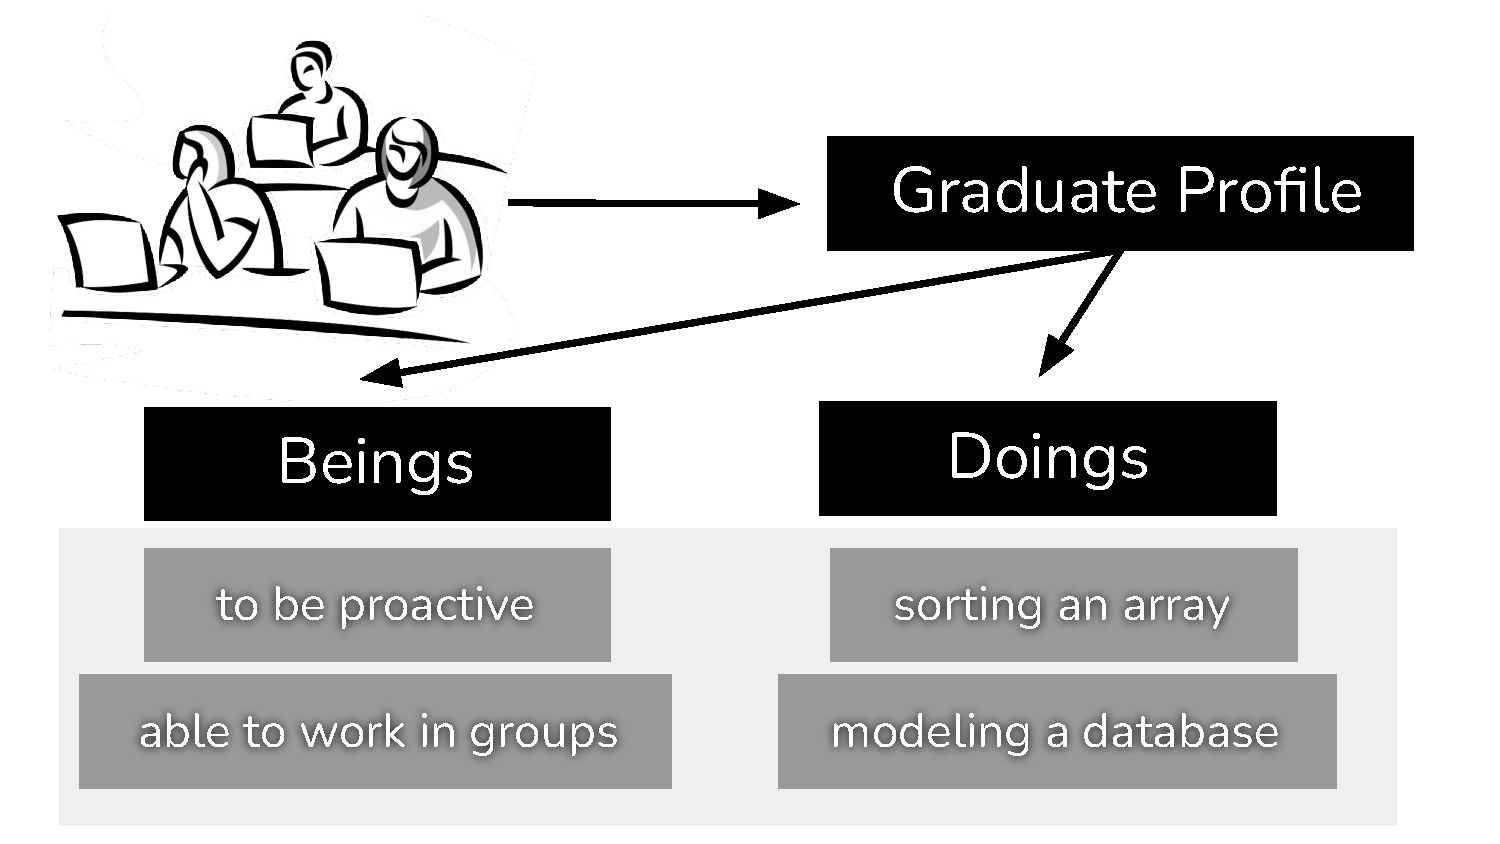
\includegraphics[width=0.9\textwidth]{images/chapter-03/graduate-profile.pdf}}
    
    \par\medskip\ABNTEXfontereduzida\selectfont\textbf{Source:} Created by the author (2024). \par\medskip
\end{figure}

A concrete example can be extracted from the \gls{CC2020} proposed by a task force conducted by \gls{ACM} and \gls{IEEE-CS}. The \gls{CC2020} \cite[p.~52]{acm:2020} embraced competency lens for all its computing curricula, giving examples of competency statements like this:  
\begin{citacao}
    "Identify and document system requirements by applying a known requirements elicitation technique in work sessions with stakeholders, using facilitative skills, as a contributing member of a requirements team".  
\end{citacao}
If we expand and rebase our way to see competency \cite{lozano:2012}, a competency can be a vector of interrelated functionings. When it is present in a political-pedagogical project, it is an expected set of functionings. When we have any graduate with this competency, it is an achieved set of functionings (or just achievement).

We know, for instance, that students only develop complex software if they have previously understood loops and conditionals. Thus, bearing in mind an achieved functioning (understood loops and conditionals) can be an expected functioning (developing complex software) in another context, it is interesting to differentiate them. Sen amplifies this difference for a freedom perspective and defines the capability concept.

\subsection{Capability}
\label{sen-ss:capability}

\citeauthoronline{sen:1992} (\citeyear{sen:1992}, pp.~39, 40) continues developing his definition as follows:
\begin{citacao}
    "Closely related to the notion of functionings is that of the capability to function. It represents the various combinations of functionings (beings and doings) that the person can achieve. Capability is, thus, a set of vectors of functionings, reflecting the person's' freedom to lead one type of life or another. Just as the so-called ''budget set'' in the commodity space represents a person's' freedom to buy commodity bundles, the ''capability set'' in the functioning space reflects the person's' freedom to choose from possible livings".    
\end{citacao}
Thus, capabilities are "the real, or substantive, opportunity that they [human beings] have to achieve these doings and beings" \cite{robeyns:2023}.

We can return to the same educational example in the previous section. Professors should conduct their students to achieve the expected functionings of the political pedagogical project. Bearing in mind that these students have a probable and different set of achievements (achieved functionings), it is possible some students may (or may not) have a vector of functionings necessary to achieve what is required by the program. If this vector of necessary functionings exists for students, we say they have capabilities for it.

Let us materialize with a concrete example. Anne, Bill, and Carla are three students who know how to develop programs satisfactorily. Anne and Bill know the Theorem of Pythagoras, but Carla does not know. The professor asks them to create a program that returns the distance between two points in a Cartesian plane after receiving the four coordinates as parameters. In a naive analysis, Anne and Bill have the capability for it, but Carla has not. Even if Bill does not want to develop what the professor asks him, he continues to have this capability. He has the freedom to do it if he wants. It does not matter if he did or not when we conduct a capability analysis.

I will complicate this situation more. Imagine that Anne wants to develop the program, but she does not have a computer in her home. She is in the middle of a critical wave of cases during a pandemic scenario like the \gls{COVID-19} one. In this aggravated situation, she does not have the capability to do it. Anne has two limitations: she does not have a computer (resource), and can not go to the lab in her university (mobility). A complete capability analysis needs to consider the complexity and multidimensionality that equity issues can achieve. To encompass this complexity that a capability analysis should have, Sen also establishes the concept of conversion factors.

\subsection{Conversion Factors}
\label{sen-ss:conv-fac}

An illustrative example helps us to understand a deeper discussion about resource provision. Figure \ref{fig:resources-conversion-factors} presents a man facing difficulties in seeing over the wall\footnote{Unknown authorship. The illustration is available in \url{https://www.reddit.com/r/brasil/comments/ 8l4qyp/dont_matter_how_much_resources_you_have_if_you/>}.}. Although he has a bunch of stairs at his disposal, he does not make use of them appropriately. There is an expression in the figure asserting that: "It doesn't matter how many resources you have… if you don't know how to use them, it will never be enough". The resource possession can not be enough to convert it into the expected benefit. 

\citeauthoronline{sen:1992} (\citeyear{sen:1992}, pp.~37, 38) asserts that there are conversion factors to be considered during a capability analysis:
\begin{citacao}
    "The resources a person has, or the primary goods that someone holds, may be very imperfect indicators of the freedom that the person really enjoys to do this or be that. [...] The personal and social characteristics of different persons, which can differ greatly, can lead to substantial interpersonal variations in the conversion of resources and primary goods into achievements. For exactly the same reason, interpersonal differences in these personal and social characteristics can make the conversion of resources and primary goods into the freedom to achieve similarly variable".
\end{citacao}
\citeonline{robeyns:2023} categorizes the conversion factors into three groups: personal, social, and environmental.

\begin{figure}[ht!]
\centering

\caption{\textmd{Illustration showing that the resource possession can not be enough to convert into the expected benefit.}}
\label{fig:resources-conversion-factors}
\fcolorbox{gray}{white}{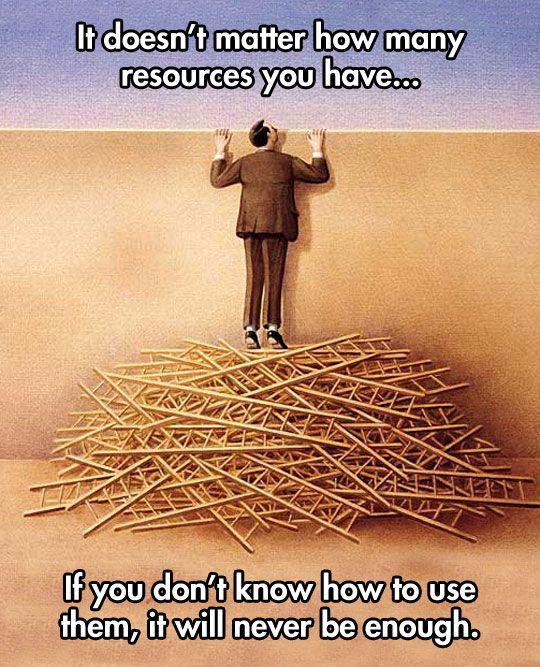
\includegraphics[width=0.6\textwidth]{images/chapter-03/resources-doesnt-matter.jpg}}

\par\medskip\ABNTEXfontereduzida\selectfont\textbf{Source:} Unknown authorship.%\citeauthor{manualufpe2020} (\citeyear{manualufpe2020}) \par\medskip
\end{figure}

Personal conversion factors "influence how a person can convert the characteristics of the commodity into a functioning" \cite[p.~99]{robeyns:2005}. I can list examples of these factors as metabolism (e.g., Do you have thyroid problems? Are you old or young?), physical condition (Are you tired? Are you disabled?), sex (e.g., Are you a woman? Are you a transgender?), reading skills (e.g., Do you know how to read? Do you know how to read English?), and intelligence (e.g., Are you competent at this? Do you have all the pre-requirements for it?). For instance, requesting \gls{CSE} students to do a reading task might not face any problem if they are well-nourished. but if they are not, we should ask ourselves what (and how) we may require of them, even knowing their food vulnerability, to respond to our requirements adequately.

Social conversion factors are directly related to the society in which people live. I can list as examples: public policies (e.g., affirmative actions, minimum income), social norms (e.g., "boys dress blue, girls dress pink", handshaking), discriminating practices (e.g., racism, homophobia), gender roles (e.g., "ladies first"), societal hierarchies (e.g., monarchy, patriarchalism), and power relations (e.g., professor-student, boss-employee). For instance, requesting \gls{CSE} students to do a reading task on Saturdays can face religious barriers. If you have one who is a member of the Seventh-day Adventist Church, this student can allegate impossibility to do this therefore Saturday is a holy day for them\footnote{By the way, I used "they/them" in this phrase to refer to someone that I do not know who is in relation to gender or sex orientation (see more in \url{https://www.npr.org/2021/06/02/996319297 /gender-identity-pronouns-expression-guide-lgbtq}). This is another example of social norm.}.

Lastly, environment conversion factors "emerge from the physical or built environment in which a person lives" \cite{robeyns:2023}. I can list as examples climate (e.g., arid, rainy), geographical location (e.g., rural, urban), proneness to natural disasters (e.g., earthquake, hurricane), and availability of natural resources (e.g., river, wood). Requesting \gls{CSE} students to go to the library to get a book immediately after a hurricane hit, for instance, can be unfeasible, and consequently, they would not have the capability for it.

I conclude this section with another \citeauthoronline{sen:1992} (\citeyear{sen:1992}, p.~38) assertion about conversion factors: 
\begin{citacao}
    "If we are interested in the freedom of choice, then we have to look at the choices that the person does in fact have, and we must not assume that the same results would be obtained by looking at the resources that he or she commands. The moves towards resource-based interpersonal comparisons in contemporary political philosophy (such as those of Rawls and Dworkin) can certainly be seen as taking us in the direction of paying attention to freedom, but the moves are substantially inadequate. In general, comparisons of resources and primary goods cannot serve as the basis for comparing freedoms".
\end{citacao}
Equality of opportunities involves resources, but not only. The \gls{CA} approach provides us with a possible common vocabulary to analyze equity issues from different theoretical standpoints. After this discussion, we can define equity as the equality of capabilities. The challenge is identifying the crucial capabilities in a \gls{CS} program and proposing policies to guarantee them.

\citeonline[p.~98]{robeyns:2005} schematizes the concepts presented here generally (Figure \ref{fig:robeyns-representation}) without educational concerns nor representing a minimal dynamic related to the flux from current to expected functionings. Bearing in mind that there is no consensus as to how methodologically operationalizing \gls{CA} constructs (e.g., \citeonline[p.~157]{comim:2008}, \citeonline[pp.~65-69]{hart:2012}), I created a minimal dynamic flux to guide an educational equity analysis from \gls{CA} lens (Figure \ref{fig:grouped-robeyns-representation}), indicating clearly three critical dimensions: Achievements (\acrshort{A}), \acrfull{M}, and Conversion Factors (\acrshort{CF}). 

\begin{figure}[ht!]
\centering

\caption{\textmd{A stylized non-dynamic representation of a person's capability set and her social and personal context.}}
\label{fig:robeyns-representation}
\fcolorbox{gray}{white}{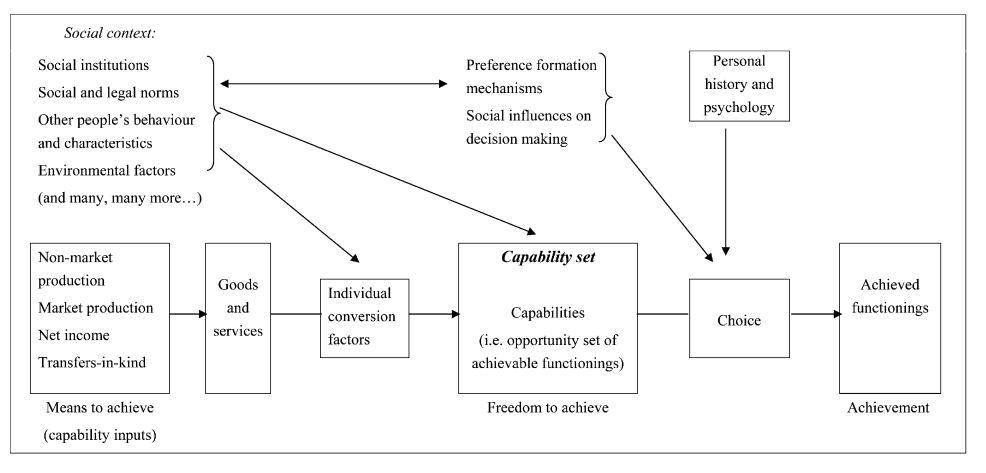
\includegraphics[width=0.9\textwidth]{images/chapter-03/robeyns-representation.png}}

\par\medskip\ABNTEXfontereduzida\selectfont\textbf{Source:} \citeonline[p.~98]{robeyns:2005}.
\end{figure}

\begin{figure}[ht!]
\centering

\caption{\textmd{A stylized dynamic representation of a student's capability set and their social and personal context.}}
\label{fig:grouped-robeyns-representation}
\fcolorbox{gray}{white}{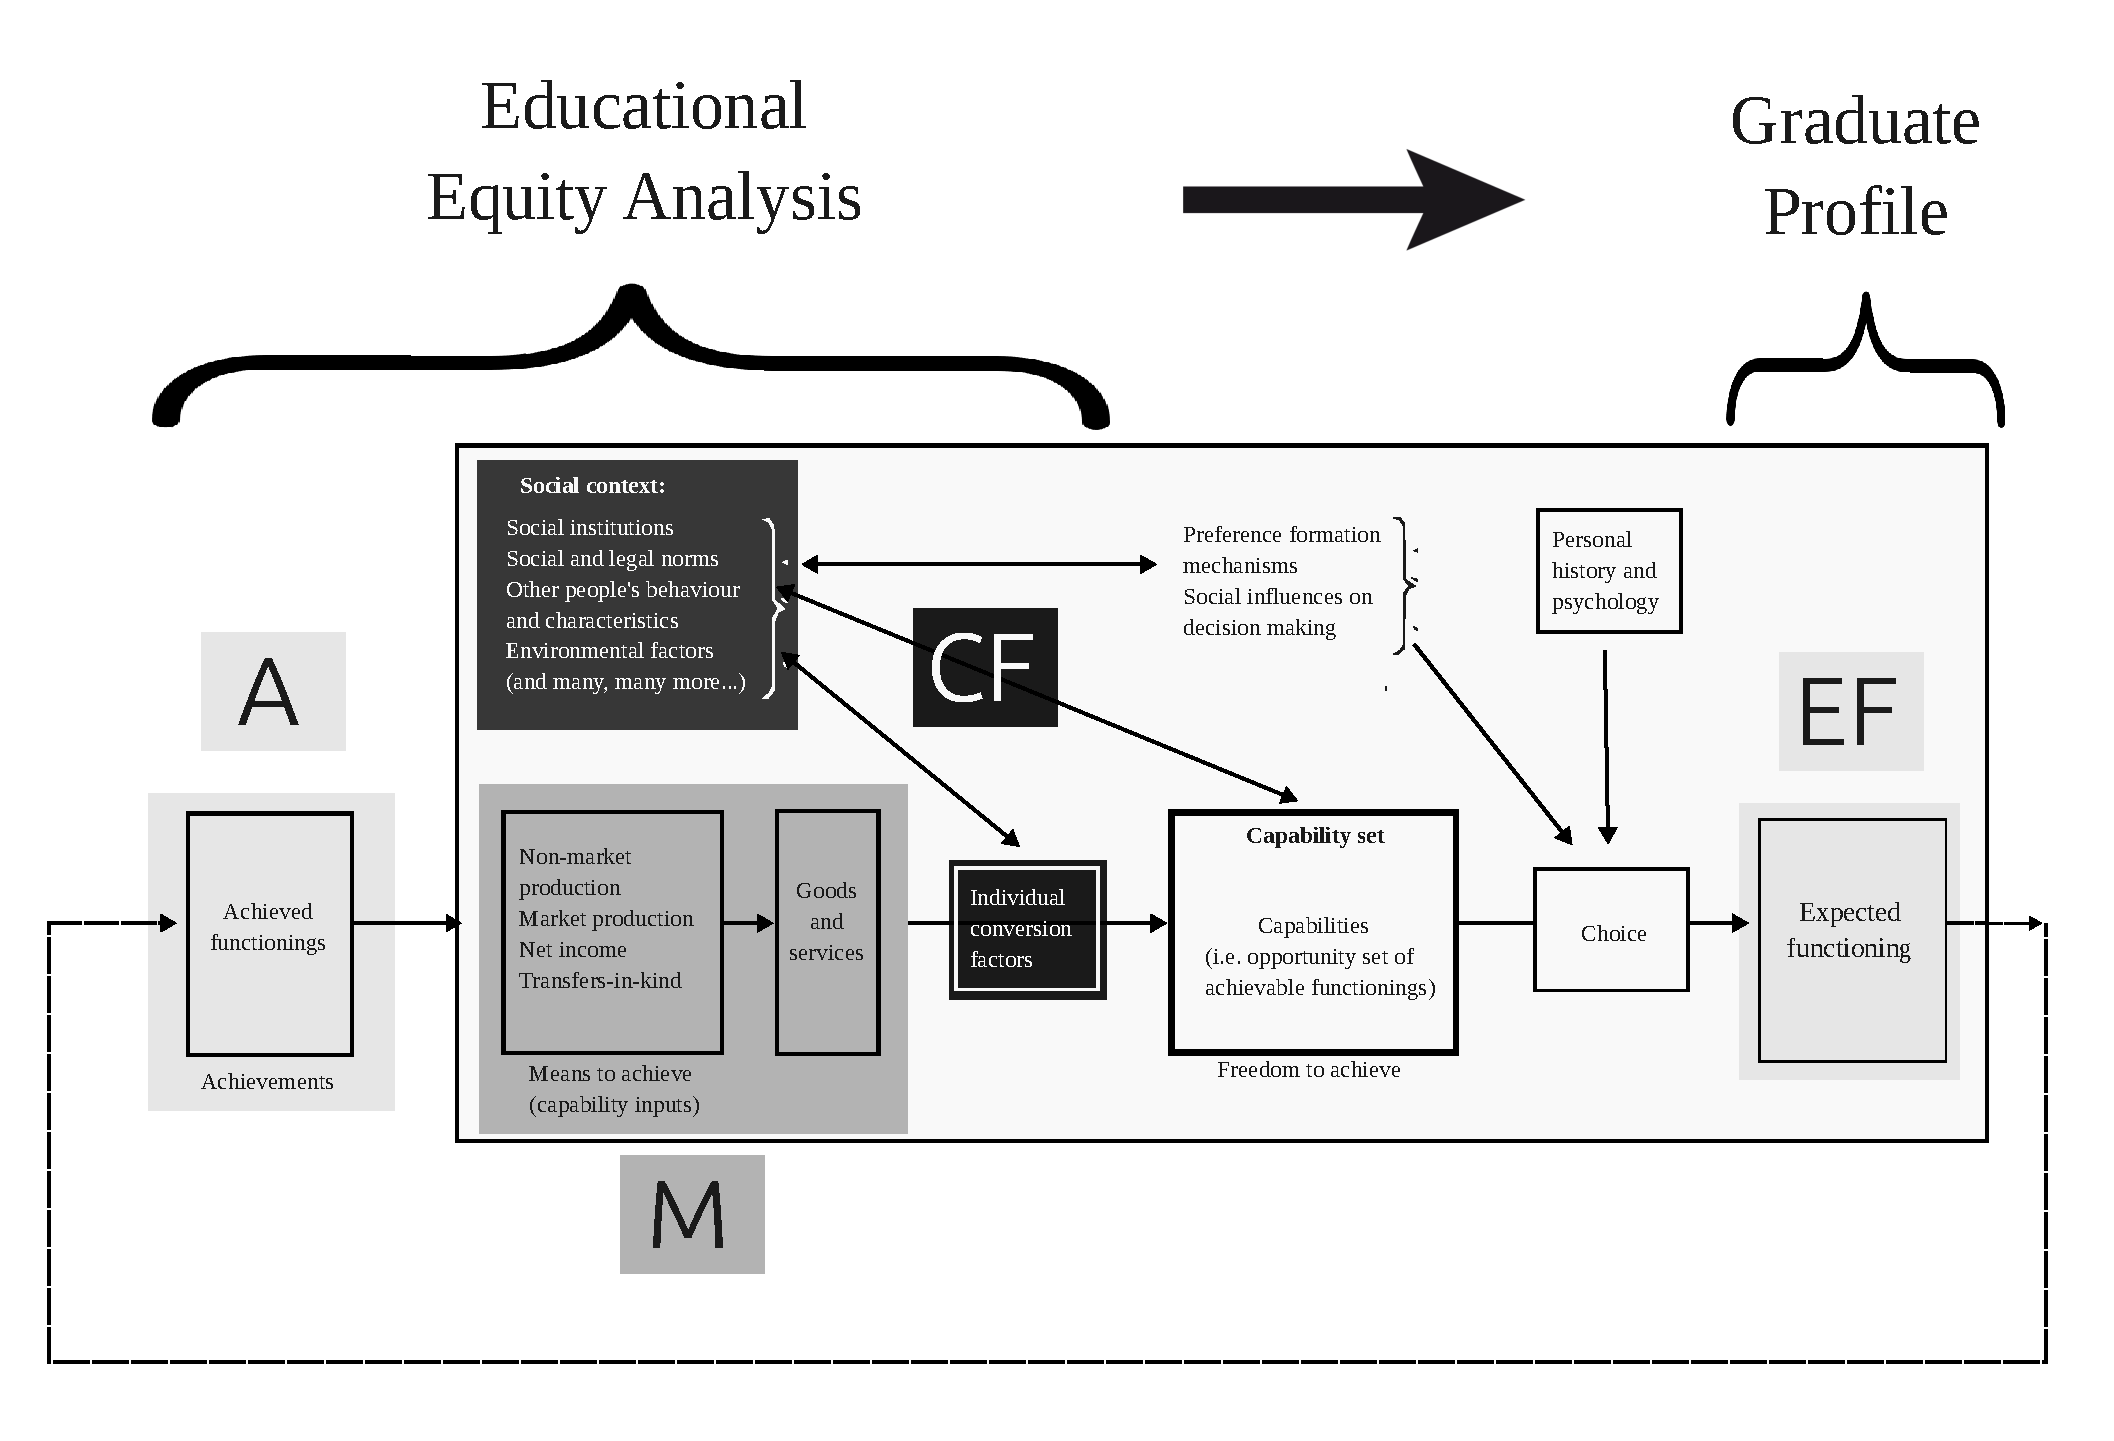
\includegraphics[width=0.9\textwidth]{images/chapter-03/grouped-robeyns-representation.pdf}}

\par\medskip\ABNTEXfontereduzida\selectfont\textbf{Source:} Created by the author (2024), adapted from \citeonline[p.~98]{robeyns:2005}.
\end{figure}

\subsection{Critiques to Capabilities Approach}
\label{sen-ss:critiques}

I can list at least two critiques to \gls{CA}. The first critique concerns the choice of a unifier lens. In the same way that Sen problematizes a resource-based lens, it is possible to extend his argument and assert that there is a level of arbitrariness in the choice of well-being as the unifier lens. Can we guarantee that this lens probably encompasses all dimensions of a complex equity analysis? Would this lens tend to value some aspects of an equity scenario more than others? Indeed, when we prefer one lens over another, our choice is carried by intentionality, and it is plausible to consider all implications of this decision. As this is a circular argument, anyone who advocates that their lens is preferable to another will be liable to suffer this kind of objection.

The second critique concerns the original \gls{CA} political standing. \gls{CA} is conceived under the liberal worldview, even situated closer to socio-liberalism. For this reason, \gls{CA} is reformist about how to proceed with the changes in our society and, consequently, not revolutionary (in a Marxist view). It is possible that some progressives or feminist researchers can not receive \gls{CA} gladly. For instance, \citeauthoronline{dejaeghere:2020} (\citeyear{dejaeghere:2020}, p.~17) approaches how postcolonial and feminist perspectives can be used to address critiques about the \gls{CA} related to questions of power and the individualized and decontextualized nature of capabilities. \gls{CA} research area is evolving the original Sen approach to appropriately consider these epistemological possibilities (e.g., critical capabilities \cite{walker:2010}).

When we presuppose a revolutionary perspective, it is essential to bear in mind the direct consequences of this choice. For instance, Figure \ref{fig:rliberation} presents a third frame proposing what should be a kind of liberation in the watching game scenario\footnote{Available by Center for Story-based Strategy (CSS) in: \url{https://www.storybasedstrategy.org/tools-and-resources}.}. The idea of providing the solution only by rearranging the box number available for each person can be read from a reformist perspective. We intervene in the box number but do not change the stadium structure, for example. The fence removal is concerned with modifying the structure at a higher level, aiming to solve this problem without recurring for a box redistribution. Although this action remedies the problem of watching games for those three people, it can generate other implicit problems that the stadium structure has already dealt with. Depending on the awareness level of the audience, the fence can play a collective role in preventing anyone from trespassing on the field and disturbing the expected flux of the game, affecting other people in the audience in their freedom to watch the game. It is totally plausible to shimmer possibilities to change the structure instead of providing only "make-up solutions" for equity problems. However, it is necessary to observe that some macro-structures in our society play multiple functions (primarily when we propose radical structural changes).

\begin{figure}[ht!]
\centering

\caption{\textmd{Illustration about the difference among equality, equity, and liberation.}}
\label{fig:rliberation}
\fcolorbox{gray}{white}{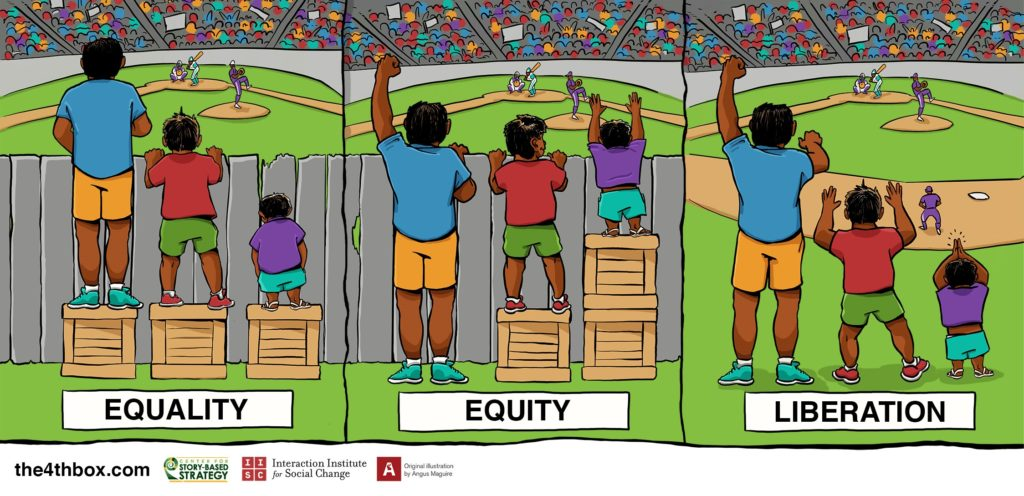
\includegraphics[width=0.9\textwidth]{images/chapter-03/liberation.jpg}}

\par\medskip\ABNTEXfontereduzida\selectfont\textbf{Source:} Unknown authorship.
\end{figure}

It is important to highlight that the reasons that I chose Rawls and Sen for this discussion in this research are (i) the agenda of social justice is not an exclusivity of progressive perspectives, and (ii) Sen contributes to this discussion from a differentiated place of speech; he is from the Global South and knows the hardness of social inequalities in his own country (India).

\section{CAPE Framework}
\label{equity-sec:cape}

\gls{CA} is one of the possible frameworks to address the balance problem of diverse sources of inequalities. But there is one of these frameworks that arises inside \gls{CEd} area and tries to address this same complex problem: \gls{CAPE} framework \cite{fletcher:2021}. It provides a set of essential constructs to conduct \gls{CEd} equity analysis to supply stakeholders with more qualified information to help their decision-making.

It stands for four expressions: \glsfirst{CAPE}. It proposes to assess \gls{CEd} using strategic questions at more diverse levels of analysis (Figure \ref{fig:cape-framework}). The \gls{CAPE} richness is that each one of these expressions represents an education level which \gls{CEd} can be offered, allowing to tackle equity issues as a public policy perspective transversally.

\begin{figure}[ht!]
\centering

\caption{\textmd{The \acrshort{CAPE} Framework schema.}}
\label{fig:cape-framework}
\fcolorbox{gray}{white}{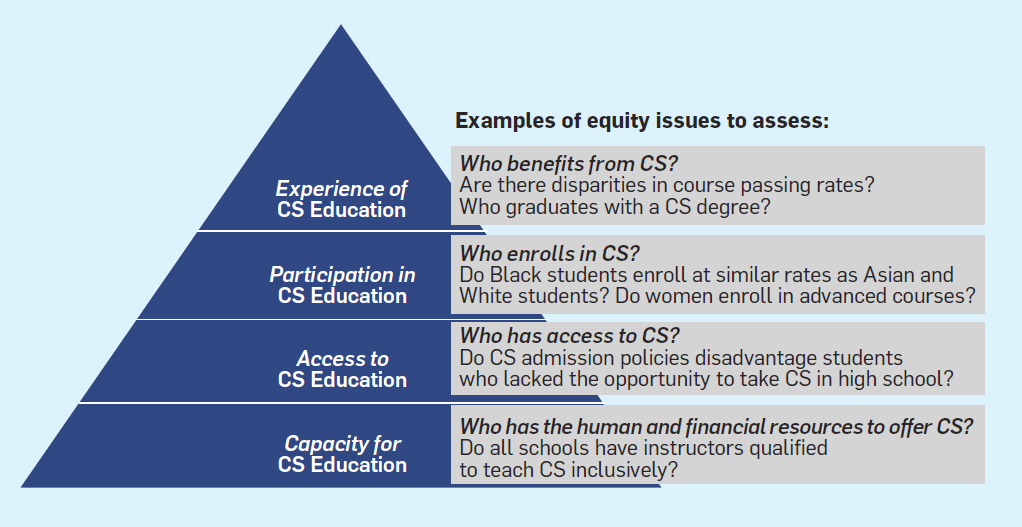
\includegraphics[width=0.9\textwidth]{images/chapter-03/cape-framework.png}}

\par\medskip\ABNTEXfontereduzida\selectfont\textbf{Source:} \citeonline{fletcher:2021}.
\end{figure}

"C" represents the capacity for offering \gls{CS} education that schools have. In this framework, it is materialized from indicators that signal to the human, material, and infrastructure dimensions. Typical questions of capacity are: "Which types of schools have teachers with the requisite skills to teach \gls{CS} courses? (ii) Do schools in low-income communities have sufficient resources to start \gls{CS} programs? (iii) Are there location-based disparities in terms of which districts are able to recruit and train \gls{CS} teachers?" \cite[p.~4]{warner:2022}.

"A" represents the access to \gls{CS} education that schools provide. While "C" represents structure, "A" represents the next step of the process: access. Both "C" and "A" refer to the basic education level. Indicators such as the number of members of disadvantaged communities who have access (or not) to \gls{CS} education. Typical questions of access are: "(i) Do \gls{CS} admission policies disadvantage students who lacked the opportunity to take \gls{CS} in high school?" (Figure \ref{fig:cape-framework}), "(ii) What is the relationship between the number of \gls{CS} courses that schools offer and the proportion of students who are economically disadvantaged?" \cite[p.~10]{warner:2022}.

"P" represents the participation in \gls{CS} education concerning the proportions of students who enrolled in \gls{CS} courses for different subgroups. Indicators such as the number of members of disadvantaged communities who participate in (or no) \gls{CS} courses. Typical questions of participation are: "(i) Do Black students enroll at similar rates as Asian and White students? (ii) Do women enroll in advanced courses?" (Figure \ref{fig:cape-framework}). 

Lastly, "E" represents the experience of \gls{CSE} students. While "P" represents participation (similar to access), "E" represents \gls{CSE} students' experience (including data related to number of egresses). Both "P" and "E" refer to the higher education level. Indicators about how "to quantitatively assess and monitor issues of equity regarding students’ learning experiences in \gls{CS}" \cite[p.~5]{warner:2022}. Typical questions of experience are: "(i) Are there disparities in course passing rates? (ii) Who graduates with a \gls{CS} degree?" (Figure \ref{fig:cape-framework}).

Although \gls{CAPE} can map important variables to an equity analysis, the concept
of 'capacity' is strongly related to resources, ignoring some essential aspects relative to the real opportunities for a computing student. Furthermore, in developing countries, other challenges emerge. Beyond the potential inequity sources that emerged from natural diversity in the classroom (e.g., gender, race), structural barriers deepen the situation (e.g., socioeconomic status, poverty). In African countries, for instance, it used the \gls{CAPE} framework to analyze equity issues in \gls{CEd} \cite{tshukudu:2023}. Although the authors highlight the strengths of its use, they also point out some limitations: 
\begin{citacao}
    ``The \gls{CAPE} framework helps map the progression from 'Capacity for' to 'Experience of' computer science education as a route to equity, but in order to support development in low and middle income countries, it may be helpful to have the capacity level finely grained'' \cite[p.~1]{tshukudu:2023}.
\end{citacao}
Maybe the \gls{CA} can help to fill some gaps during equity analysis using only the \gls{CAPE} framework. 
\section{Brazilian Context of Higher Education}
\label{equity-sec:br-context}

In 2022, Brazil offered more than 22 million vacancies in higher education. Only 3.81\% of these vacancies were in the public educational system, revealing that 74.74\% of more than 22 million vacancies referred to online education in the private educational system. When we restrict these vacancies to in-person higher education (more than 5 million), this percentage increases to 13.48\% in the public educational system, still indicating the scarcity of the public good that is the access to public higher education at Brazil\footnote{Data collected from the presentation for the press conference of \gls{INEP} about the 2022 Brazilian Higher Education Census (Slide 20). See more in the Brazilian Portuguese reports available in \url{https://www.gov.br/inep/pt-br/areas-de-atuacao/pesquisas-estatisticas-e-indicadores/censo-da-educacao-superior/resultados}.}.

High school graduates are natural candidates to dispute these higher education vacancies. In 2023, 83.56\% of Brazilian fresh students in high school were in public educational institutions, whereas 16.44\% were in private ones\footnote{Data collected from the presentation for the press conference of \gls{INEP} about the 2023 Brazilian School Census (Slide 26). See more in the Brazilian Portuguese reports available in \url{https://www.gov.br/inep/pt-br/areas-de-atuacao/pesquisas-estatisticas-e-indicadores/censo-escolar/resultados}.}. It is probable that the most part of higher education candidates are from public educational system but, intriguingly, the offering of higher education vacancies in this public system is scarce. Thus, it seems that Brazilian public higher education is a not-abundant common good, being necessary to create ways of how the society could better benefit from it.

Another critical perspective concerning income distribution in Brazil \cite{sasse:2021}. Only 1\% of richest people holds on 23.3\% of national income, while 40\% of poorest one holds only 10.4\%. This means that the 1\% of  the richest parcel of Brazilian population has the double of income of 40\% of poorest one. These values puts Brazil at the second place on the list of 180 countries with more income concentration in the world (only behind Qatar).

Bearing this scenario in mind, since 2013, the Brazilian Ministry of Education\footnote{See more detail in the \gls{MEC} official site: \url{http://portal.mec.gov.br/cotas/sobre-sistema.html}.} adopts system of quotas in all federal educational institutions. One of the principles is avoiding what \citeonline[p.~32]{bourdieu:2013} called "school as a conservative force", giving crucial steps for a more equitable educational system that can promote the school as a factor of social mobility. In Brazilian federal higher institutions, 50\% of vacancies are reserved for high school graduate candidates from public institutions. Inside each half of vacancies, it applies other criteria in this order: \gls{HPCI}, race/ethnicity, and disableness. The 2023 Brazilian Higher Superior Census, concerning federal students, reveals that 51\% that came from the system of quotas finished their undergraduate studies, while this rate is 41\% from other students\footnote{Available as news from \gls{INEP} site: \url{https://www.gov.br/inep/pt-br/assuntos/noticias/censo-da-educacao-superior/mec-busca-garantir-permanencia-de-estudantes-mais-vulneraveis}.}.
\section{Equity and Active Methodologies in CEd}
\label{equity-sec:active-learning}

Parents tackle some situations to guarantee an environment with fewer disputes among their children. Imagine the scenario where we have a parent, two children, and a bar of chocolate. This parent has the following question: How to teach your children to find the best way to divide a bar of chocolate between them?

A possible way to solve this problem is this parent follows the approach: (i) dividing the bar into two equal parts, and (ii) giving each part to each one.  Although it seems fair, this parent would make the whole process and not allow the children to learn in this situation. In addition, (s)he would be the ruler and be obliged to handle possible objections of a wrong division made in step (i).
This parent can use an alternative way to solve this problem. There is an approach called “cut-and-solve”. It consists of just two steps: (i) one child cuts the bar, and (ii) another one chooses a piece. Thus there are a divider and a chooser. The divider will not choose, and the chooser will not divide. This approach is a good idea because this parent solves one drawback: (s)he would not be the divider (because that who divides can fail to perform a precise division). But an important something remains: (s)he has been the ruler yet.

The first way seems more authoritarian, although it attends to fair principles. But the alternative way seems more respectful and guarantees other things beyond fairness. This guarantees (i) the reflection of equitable variables trade-off, (ii) a discovery learning solution, and (iii) the promotion of democratic values. The “cut-and-solve” approach is an old (and an excellent) solution for some cases of simple fair division problems \cite{brams:2020}. Academic papers have formally addressed this issue since 1948 (e.g., \citeonline{steinhaus:1948}).

In \gls{CEd}, several works approach equity in active learning contexts from pair programming use. \citeonline{lewis:2015}, for instance, identified patterns of marginalization and domination between the pairs. Beyond dominance \cite{grabl:2024}, more recent papers investigated other equity issues like gender \cite{bodaker:2023}, refugees \cite{arawjo:2021}, and sense of belonging \cite{izhikevich:2022}.

I explored other challenges in this subject through a fictitious story\footnote{This story was written originally in Brazilian Portuguese in this essay \cite[pp.~277,278]{bispojr:2022-educomp}.}: 
\begin{citacao}
    "Professor Quincas Borba is very happy with the use of active approaches. He realizes that there is more enthusiasm in his classroom in a general way. Several students like to attend and participate in his classes. He also realizes that many of his students can solve real problems involving data structures in a way that the proportion of competent students to do this is higher than before when he used the expositive format more strongly in his classes. The students complained about the higher workload that they need to do now, but, in a general way, they approved the changes made by him.

    However, Prof. Quincas is disturbed by a specific scenario in his classroom. There is a group of students that is not adapting well to this new approach. Among these students, two are of special interest: Lindoia and Brás. Lindoia is a joyful student and looks to demonstrate a certain interest in her studies. However, she is a little introverted. She entered the Computing program by affirmation policies as an indigenous person. Brás is a guy who clearly demonstrates his desire to learn just by seeing his facial expression. He has an easy smile and likes to be quite cordial. He does classroom activities always together with his faithful partner, Capitu, his sign-language interpreter. He is deaf-mute.

    Prof. Quincas finds himself in a quite hard and challenging situation. His active methodologies require a certain dynamism in the activity conduction. This rhythm is necessary for the moments of group discussion, alternating with individual and gamification moments, which play the role of involving the students in a favorable and stimulating learning environment. However, Lindoia and Brás have many difficulties in actively participating in activities. Due to both situations, the language flow is not performed satisfactorily because Lindoia and Brás do not have Portuguese as their native language but as a second one. So, in activities in which Lindoia and Brás participate, they always leave behind flux, as suggested by Prof. Quincas. They make an effort to follow activities. Lindoia makes a higher cognitive effort to live together in an educational space where everybody does not speak Guarani\footnote{Indigenous language from the South part of South America spoken by people from Tupi-Guarani ethnicity.}. Brás keeps his fingers crossed for the effort and dedication of Capitu can, as quickly as possible, understand the speech content of his colleagues and Prof. Quincas and make the interpretation in Brazilian Sign Language for him (and vice versa). As the dynamic cools down in scenarios like this, Prof. Quincas also realizes that there is no natural disposition of other students to want to participate in groups when Lindoia and Brás are present".
\end{citacao}
These challenges need to be more investigated in \gls{CSE} contexts, mainly in Brazilian ones. \citeonline{murray:2024} reported an excellent qualitative study from \gls{SLICC}, but in an interdisciplinary way and not focused on \gls{CEd}.

% \vspace{0.3cm}

% \fbox{
%     \begin{minipage}[htb]{0.9\textwidth}
%         \vspace{0.3cm}
                
%         \colorbox{gray!30}{% create a colored box
%             \makebox[0.975\textwidth][l]{% center the text on the page
%                 \ \ \textbf{Further Writing}
%             }
%         }

%         \vspace{0.1cm}
        
%         \begin{itemize}
%             \item Presenting the \citeonline{lewis:2015} paper.
%             \item Including that fictitious story created by me \cite{bispojr:2022-educomp}.
%             \item Presenting the potential of active methodologies to promote social justice.
%             \item Highlighting that SDL is weakly investigated in this direction.
%         \end{itemize}

%         \vspace{0.25cm}
        
%     \end{minipage}
% }

  
\chapter{Related Work}
\label{chap:rel-work}

 There are various reasons to structure a related work chapter \cite[p.~14]{booth:2016-slr}. For this thesis, I am interested in (i) locating my work within the existing literature and (ii) justifying its originality. Doing this in a qualitative investigation requires me to establish some considerations.
 
Although the expression “on the shoulders of giants” can represent a humble stance before the complexity and greatness of produced knowledge through scientific endeavor, it is possible to interpret it in a positivist way. The discussion proposed here does not intend to build one brick more in a cartesian wall of science. I propose to establish one more link to the big network of produced scientific knowledge. In this network, each node links a perception of reality historically, through dialogues with the contribution of colleagues situated in space and time.

In this perspective, it is necessary to move away from a kind of technicism that tries to specify and discretize every step of a given methodology. A hidden pitfall is to use this agenda to describe reality, just as it is, in a positivist way. What we need is a rigorous and, if possible, systematic description to explicit the main aspects of our methodological approach. A systematic approach in a qualitative research is not strictly a matter of reproducibility, like we try to replicate an experiment. However, it is a concern of rigor that legitimizes the quality of our research and allows other researchers to structure a possible transferability (see more in Chapter \ref{chap:res-methodology}).

One of these pitfalls is the own systematization process. There is a particular fear among qualitative researchers that the emergence of findings during and after the data collection, for instance, can be harmed due to the process inflexibility. About it, \citeauthoronline{meinefeld:2004} points out:
\begin{citacao}
    “[...] this does not mean that the result has been predetermined, as critics sometimes claim: it is only the framework of the dimensions involved in the investigation that has been fixed, but not their concrete manifestations of content.” \cite[p.~157]{meinefeld:2004}.
\end{citacao}

Understanding and admitting that not every systematic approach contributes negatively to rigorous and well-conducted qualitative research is necessary. A systematic approach can provide a solid foundation to help other researchers adequately posit their investigation into the major network of produced knowledge. In this thesis, I use a systematic mapping instead of a systematic review. \citeonline[p.~1]{petersen:2015} establish the distinction between them:
\begin{citacao}
    “While systematic reviews aim at synthesizing evidence, also considering the strength of evidence, systematic maps are primarily concerned with structuring a research area”.    
\end{citacao}

Systematic reviews tend to be more committed to the movement of evidence-based science, quantifying and discretizing this process overly. Systematic maps pervade several research perspectives and allow to structure a related work to qualitative research without leaving essential aspects in this approach.

In summary, I can retake the aims of this systematic mapping and assert that (i) \underline{locating my} \underline{work within the existing literature} is important not only for situating this research but also to help other researchers to situate their further works, and (ii) \underline{justifying its originality} in a qualitative approach is, above all, evidencing the need to uncover the implicit meaning in a concrete context. 

The remainder of the chapter is organized as follows. Section \ref{rel-work:scoping-snowball} presents the scoping study aligned with the snowballing strategy. Important elements of a systematic map such as research questions (Section \ref{rel-work:res-questions}), snowballing start set (Section \ref{rel-work-ss:start-set}), and inclusion and exclusion criteria (Section \ref{rel-work-ss:inc-exc-criteria}) are detailed. Section \ref{rel-work-ss:first-iterations} describes the first two snowballing iterations, showing both backward and forward steps. At last, after charting data (Section \ref{rel-work:charting-data}), Section \ref{rel-work:sum-results} exposes the data analysis of these iterations, situating this thesis into a general frame of the research area.

\section{Scoping Study with Snowballing Strategy}
\label{rel-work:scoping-snowball}

A systematic mapping used to be a good starting point for further research \cite{kitchenham:2011}, including for Ph.D. studies \cite{kitchenham:2010}. In this mapping, I follow the general framework of a scoping study \cite{arksey:2005}, considering the guidelines for snowballing in systematic literatures proposed by \citeonline{wohlin:2014}. I will describe them better as follows.

The scoping study is a systematic mapping that aims “to map rapidly the key concepts underpinning a research area and the main sources and type of evidence available, [...] especially where an area is complex or has not been reviewed comprehensively before” \cite[p.~21]{arksey:2005}. The methodological framework of a scoping study can be divided into five stages: (i) identifying the research question, (ii) identifying relevant studies, (iii) study selection, (iv) charting data, and (v) collating, summarizing and reporting the results \cite[p.~22]{arksey:2005}.

For identifying relevant studies (second stage), I use the snowballing strategy as the main road to locate additional papers to include for further selection and analysis. This inclusion can be via the reference list or the citations of a paper. The process of identifying new papers from the references’ and the citations’ list are commonly called backward and forward snowballing \cite[p.~1]{wohlin:2014}. Figure \ref{fig:snowballing-schema} presents this procedure schematically. It is important to highlight that several computing education researchers use snowballing strategy in their systematic literature studies as \citeonline{qian:2017}, \citeonline{gomes:2020} and \citeonline{indriasari:2020}.

\begin{figure}[ht!]
\centering

\caption{\textmd{Snowballing procedure schema.}}
\label{fig:snowballing-schema}
\fcolorbox{gray}{white}{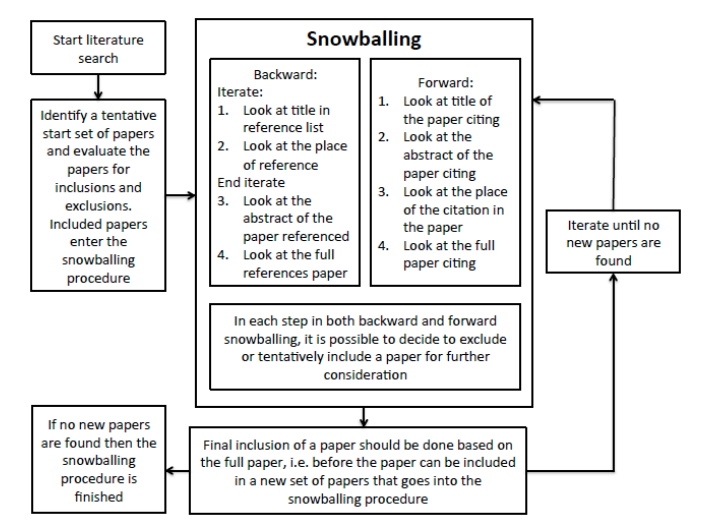
\includegraphics[width=0.9\textwidth]{images/chapter-04/snowballing-schema.png}}

\par\medskip\ABNTEXfontereduzida\selectfont\textbf{Source:} \citeonline{wohlin:2014}.
\end{figure}
\section{Identifying the Research Questions}
\label{rel-work:res-questions}

My \gls{MRQ} is “how do \gls{CSE} students conduct their \gls{SDL} in developing countries from the lens of the capabilities approach?” (stated before in Chapter \ref{chap:intro}). However, aiming to situate my project into a broad network of the research area, I use a \gls{SRQ}: “which and how are the works in \gls{CEd} involving equity issues and active learning?”. In order to address the research question we consider four \glspl{DSRQ}:
\begin{itemize}
    \item What are research methodologies (or kind of review, being a secondary work) used? (\gls{DSRQ}.1);
    \item What are the contexts (country, education level) involved? (\gls{DSRQ}.2);
    \item What are the equity issues investigated? (\gls{DSRQ}.3); and
    \item What are active approaches adopted? (\gls{DSRQ}.4).
\end{itemize}

When I refer to active learning, I use the general definition of \citeonline{bonwell:1991}, which assert that it is “anything that involves students in doing things and thinking about the things they are doing” \cite[p.~19]{bonwell:1991}. The authors mention that there is no precise definition of active learning (as also \citeonline[p.~223]{prince:2004}), but some general characteristics can be listed as:
\begin{itemize}
    \item “Students are involved in more than listening;
    \item Less emphasis is placed on transmitting information and more on developing students’ skills;
    \item Students are involved in higher-order thinking (analysis, synthesis, evaluation);
    \item Students are engaged in activities (e.g., reading, discussing, writing);
    \item Greater emphasis is placed on students’ exploration of their own attitudes and values” \cite[p.~19]{bonwell:1991}.
\end{itemize}


\section{Study Selection}
\label{rel-work:study-selection}

\subsection{Start Set}
\label{rel-work-ss:start-set}

My start set is composed of a single paper entitled “How equity and inequity can emerge in pair programming” \cite{lewis:2015}. This paper was cited in an important review in the Cambridge Handbook of Computing Education Research \cite{lewis:2019} and pointed out the gaps and challenges in equity and diversity. This review points to the challenge of considering equity issues and active learning in \gls{CSE}.

\subsection{Inclusion and Exclusion Criteria}
\label{rel-work-ss:inc-exc-criteria}

I used a single \gls{IC} that was “The work attends to \gls{SRQ}”. In this systematic mapping, all the exclusion criteria served as common reasons to justify the paper exclusion. The \gls{EC} are listed as follows.
\begin{itemize}
    \item The work does not approach Computing Education (\gls{EC}1);
    \item The work does not approach equity (\gls{EC}2);
    \item The work does not approach active methodology (\gls{EC}3);
    \item The work approaches \gls{CEd}, equity, and/or active methodology but does not interlink (\gls{EC}4); and
    \item The work does not fit in the range from 2020 to 2024 (\gls{EC}5).
\end{itemize}

My strategy used each \gls{RC} as follows: (i) title and abstract (\gls{RC}1); (ii) work scanning (\gls{RC}2); and full reading (\gls{RC}3). When \gls{RC}1 failed to exclude the paper, it followed \gls{RC}2. If both criteria were passed, this paper became a real candidate, and we performed \gls{RC}3. 

\subsection{First Iterations}
\label{rel-work-ss:first-iterations}

I conducted two iterations of the snowballing strategy with the specifications described before. I will detail this in the next sections.

\subsubsection{Iteration 0}

This iteration did not backward any paper because the single work in this current start set \cite{lewis:2015} is dated 2015, being all references before 2020 (falling into \gls{EC}5). However, the forward process returned eleven papers after applying \gls{EC} filtering. The search engine used for the generation of the citation list was the Scopus Base, retrieving the last results on July 19, 2024. Figure \ref{fig:first-iteration} presents the diagram of the whole iteration.

\begin{figure}[htb]
\centering

\caption{\textmd{Diagram of Iteration 0 after snowballing strategy.}}
\label{fig:first-iteration}
\fcolorbox{gray}{white}{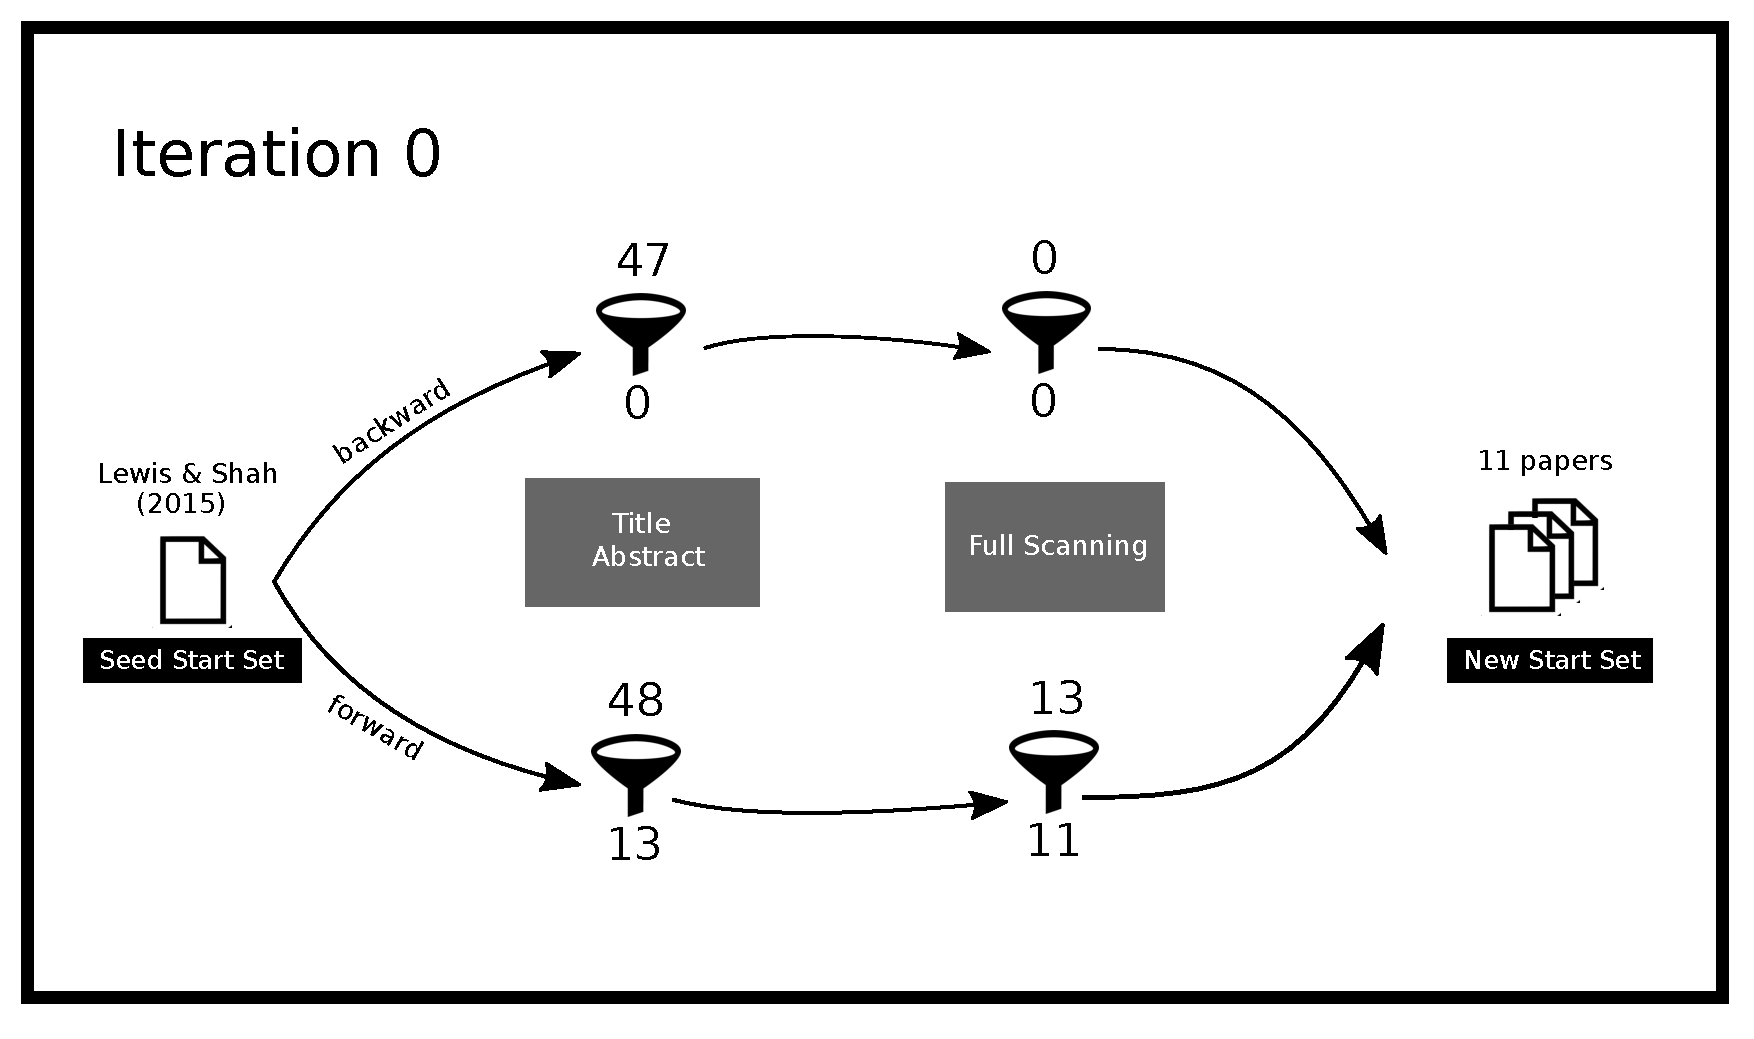
\includegraphics[width=0.95\textwidth]{images/chapter-04/first-iteration.pdf}}

\par\medskip\ABNTEXfontereduzida\selectfont\textbf{Source:} Created by the author (2024).
\end{figure}

Thus, at the end of this iteration, the paper set increased from one to eleven papers (see Table \ref{tbl:iteration-0-list-papers}), bearing in mind that the work \cite{lewis:2015} was chosen strategically, aiming to capture newer works after 2020 (inclusive).

\begin{table}[htb]
\caption{List of the papers of the new start set identified during the 
Iteration 0 after snowballing strategy.}
\label{tbl:iteration-0-list-papers}
\centering
\rowcolors{1}{}{lightgray}
\begin{tabular}{
    m{7cm}|
    m{7cm}
}
    \hline
    \multicolumn{2}{c}{
        \textbf{Seed Start Set}
    }\\
    \hline
    \multicolumn{2}{c}{
        \citeonline{lewis:2015}
    }\\   
    \hline
    \multicolumn{2}{c}{
        \textbf{New Start Set}
    }\\
    \hline
    \citeonline{arawjo:2021} &
    \citeonline{ayub:2020} \\

    \citeonline{bodaker:2023} &
    \citeonline{grabl:2024} \\
    
    \citeonline{gransbury:2022} &    
    \citeonline{izhikevich:2022} \\
    
    \citeonline{love:2021} &    
    \citeonline{lui:2020} \\
    
    \citeonline{lyttle:2020} &    
    \citeonline{musaeus:2022} \\
    
    \citeonline{ying:2021} &
    \\
    \hline
    
\end{tabular}

  \par\medskip\ABNTEXfontereduzida\selectfont\textbf{Source:} Created by the author (2024). \par\medskip
\end{table}

\subsubsection{Iteration 1}

The backward process of Iteration 1 returned 11 papers after applying \gls{EC} filtering. In the next step, the forward process returned 9 papers after applying \gls{EC} filtering. The search engine used for the generation of the citation list was also the Scopus Base, retrieving the last results on July 22, 2024. Figure \ref{fig:second-iteration} presents the diagram of the whole iteration.

Thus, at the end of this iteration, the paper set increased from 11 to 31 papers (see Table \ref{tbl:iteration-1-list-papers}). I released all detailed information about the study selection in an online public repository\footnote{The snowballing information of this mapping is available on this \gls{Ph.D.} public repository: \url{https://github.com/bispojr/phd-info}.}, structuring through a spreadsheet with all decisions made in this stage.

\begin{figure}[htb]
\centering

\caption{\textmd{Diagram of Iteration 1 after snowballing strategy.}}
\label{fig:second-iteration}
\fcolorbox{gray}{white}{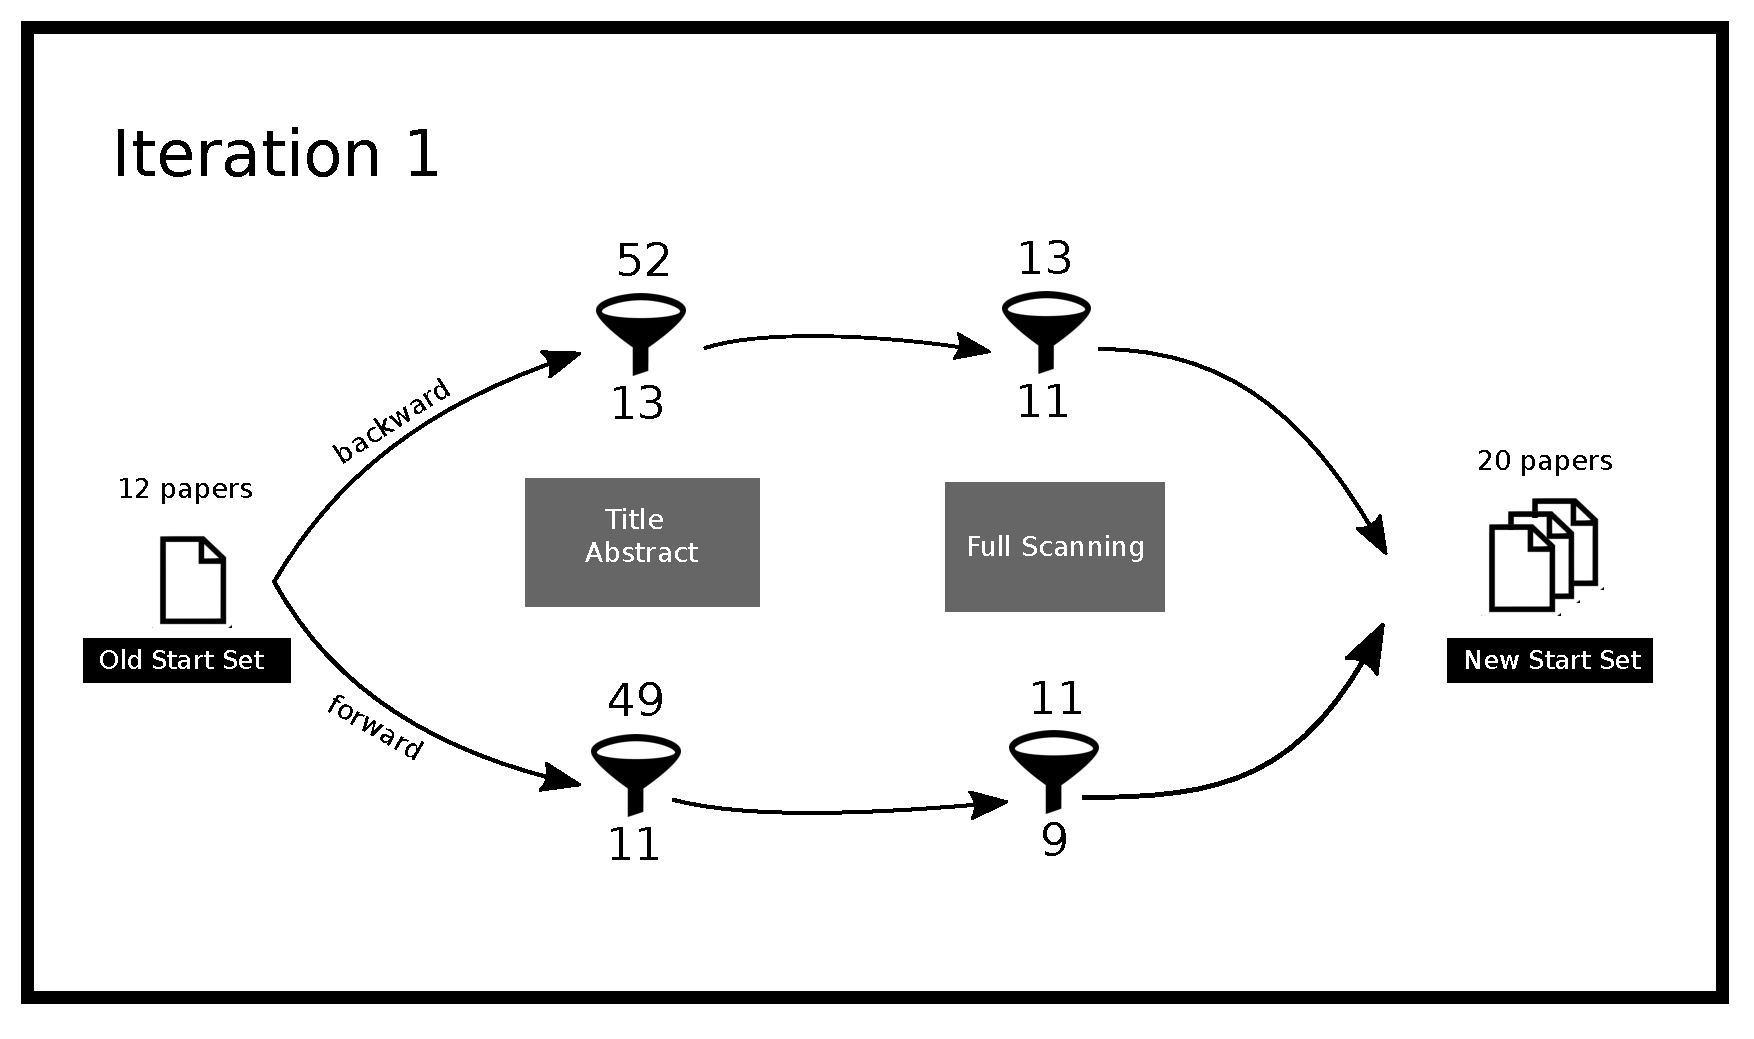
\includegraphics[width=0.95\textwidth]{images/chapter-04/second-iteration.pdf}}

\par\medskip\ABNTEXfontereduzida\selectfont\textbf{Source:} Created by the author (2024).
\end{figure}
\section{Charting Data}
\label{rel-work:charting-data}

I created a list of essential items of information that should be obtained from selected papers from the first iterations. This list helped me to arrange the works and situate how the area is being explored and which potential gaps and challenges should be addressed. Each item has a related \gls{DSRQ}, contributing to answer \gls{SRQ}. Table \ref{tbl:papers-chart} details this list.

\begin{table}[htb]
\caption{List of the papers of the new start set identified during the 
Iteration 1 after snowballing strategy.}
\label{tbl:iteration-1-list-papers}
\centering
\rowcolors{1}{}{lightgray}
\begin{tabular}{
    m{7cm}|
    m{7cm}
}
    \hline
    \multicolumn{2}{c}{
        \textbf{Old Start Set}
    }\\
    \hline
    \citeonline{arawjo:2021} &
    \citeonline{ayub:2020} \\

    \citeonline{bodaker:2023} &
    \citeonline{grabl:2024} \\
    
    \citeonline{gransbury:2022} &    
    \citeonline{izhikevich:2022} \\
    
    \citeonline{love:2021} &    
    \citeonline{lui:2020} \\
    
    \citeonline{lyttle:2020} &    
    \citeonline{musaeus:2022} \\
    
    \citeonline{ying:2021} &
    \\
    \hline    
    \multicolumn{2}{c}{
        \textbf{New Start Set}
    }\\
    \hline
    
    \citeonline{akalin:2021} &
    \citeonline{alvarado:2022} \\
    \citeonline{bowman:2020} &
    \citeonline{broll:2021} \\
    \citeonline{demir:2021} &
    \citeonline{eglash:2020} \\
    \citeonline{goode:2021} &
    \citeonline{kung:2022} \\
    \citeonline{lai:2023} &
    \citeonline{lott:2021} \\
    \citeonline{michaelis:2022} &
    \citeonline{nakai:2023} \\
    \citeonline{roque-hernandez:2021} &
    \citeonline{shahin:2022} \\
    \citeonline{su:2023} &
    \citeonline{tan:2024} \\
    \citeonline{toro:2024} &
    \citeonline{tseng:2024} \\
    \citeonline{wei:2021} &
    \citeonline{ying:2021b} \\

    \hline
    
\end{tabular}

  \par\medskip\ABNTEXfontereduzida\selectfont\textbf{Source:} Created by the author (2024). \par\medskip
\end{table}

\begin{table}[htb]
\caption{List of items of information obtained from the selected papers during the first iteration. Each item has a related derived secondary research question.}
\label{tbl:papers-chart}
\centering
\rowcolors{1}{}{lightgray}
\begin{tabular}{
    m{2.5cm}|
    m{7cm}|
    m{3cm}
}
    \hline
    \multicolumn{2}{c}{Item of Information} &
    Related \gls{DSRQ}\\
    \hline
    Research &
    Type & \gls{DSRQ}.1 \\
    & Kind & \gls{DSRQ}.1 \\
    & Methodology & \gls{DSRQ}.1 \\
    \hline
    Context &
    Educational Level & \gls{DSRQ}.2 \\
    & Country / Region & \gls{DSRQ}.2 \\
    \hline
    Equity & 
    Equity Issue & \gls{DSRQ}.3 \\
    & General Equity Theory / Framework & \gls{DSRQ}.3 \\
    \hline
    - &
    Active Learning Approach & \gls{DSRQ}.4\\
    \hline
    
\end{tabular}

\par\medskip\ABNTEXfontereduzida\selectfont\textbf{Source:} Created by the author (2024). \par\medskip

\end{table}

The filled data chart from 31 papers is available in Appendix \ref{chap:data-charting}. I used this charting not only to answer \gls{SRQ} but to situate \gls{MRQ} in the broader area, as will be seen in the next section.
\section{Summarizing and Situating Results}
\label{rel-work:sum-results}

In this section, I present the summary of the results, positioning my research before the broader area (Section \ref{rel-work-sum-ss:summary}) and some of the mapping threats (Section \ref{rel-work-sum-ss:threats}).

\subsection{Summary and position}
\label{rel-work-sum-ss:summary}

\subsubsection{Research (DSRQ.1)}

About \gls{DSRQ}.1, most of the papers are primary works (29). There is only (i) one secondary paper \cite{lai:2023}  that reviews the broader area from the \gls{SRQ} perspective and (ii) one essay \cite{michaelis:2022} that is usually in frontiers between primary and secondary categories. There is a reasonable balance between quantitative (10), qualitative (8), and mixed-methods (10) approaches. It was not possible to identify the research methodology in two papers \cite{michaelis:2022,akalin:2021} and the secondary work used the \citeonline{kitchenham:2007} guidelines.

I chose a primary and qualitative approach for this research project. This option reflects the research that looks for a better understanding of real scenarios when inequalities of opportunity can arise. I conducted a basic qualitative research using quantitative data to support triangulations and sampling choices.

\subsubsection{Context (DSRQ.2)}

In relation to \gls{DSRQ}.2, the papers are balanced into higher (14, including graduate studies) and basic education (13, including high school and professional formation). The possible reason for this equilibrium is the inclusion of computing in basic education in many countries. The work of \citeonline{arawjo:2021} is an example of an exception, focusing on informal education (3) too. Most papers investigate the research context in \gls{USA} (16), followed by Asia (6), and Europe (5). Africa \cite{arawjo:2021}, Latin America \cite{roque-hernandez:2021}, and Oceania \cite{shahin:2022} have only one work each.

I investigated \gls{CSE} context in this thesis. However, the Brazilian scenario brings a difference when focusing on developing countries. Only seven papers (of 31) have their contexts situated in the Global South\footnote{I used the demarcation criteria adopted by \gls{BISA}. See more in \url{https://www.bisa.ac.uk/become-a-member/global-south-countries}.}. Only one of them investigates Latin American contexts \cite{roque-hernandez:2021}, for instance. There is a need for more research in developing countries into this cut.

\subsubsection{Equity (DSRQ.3)}

About \gls{DSRQ}.3, the papers approach a wide range of equity issues prevailing gender (13), performance (10, including self-efficacy and expertise), and race (7, including culture and nationality) issues. Few works investigated sense of belonging (2), participation (2), and access (1) issues. In relation to a general equity theory (or framework), no work uses a consolidated theory/framework, usually building its theoretical background from various constructs spread over several references. In this perspective, four works drew my attention concerning their theoretical background, highlighting  intercultural computing \cite{arawjo:2021} that resulted from a specification of a previous theory (intercultural learning). Other three works refer to epistemic injustice \cite{love:2021}, gender gap \cite{bodaker:2023}, and interest development theory \cite{michaelis:2022}.

This research used the \gls{SES} to help to choose participants during data collection. However, the thesis's uniqueness resided in using a general equity theory / framework, allowing me to investigate a Brazilian context under well-informed and general equity constructs. A crucial characteristic of my research is using \gls{CA} as an equity framework. The richness of this choice increases when we consider the singular reality faced by developing countries, deepening the discussion of the deprivation of freedoms and not only about the presence/lack of resources. 

\subsubsection{Active Approach (DSRQ.4)}

At last, in relation to \gls{DSRQ}.4, most of the papers investigated collaborative learning (25), being pair programming the major part. Few works adopted other approaches like \gls{PBL} (2), peer-mentoring (2), mixed-approaches (2), and project-based learning (1).

I looked into the \gls{SDL} as an active approach. The potentiality of my research was focusing on a more general approach (\gls{SDL}) than a specific one (e.g., andragogy, \gls{PBL}). Although I investigated a Brazilian context with a \gls{PBL} scenario,  the understanding of \gls{SDL} is crucial because it dialogues and is part of several other active approaches (see Section \ref{sdl-sec:relations}).

\subsection{Mapping Threats}
\label{rel-work-sum-ss:threats}

I list three main threats of this scoping study. First, I conducted only the first two iterations of snowballing until now. It is usually necessary to finish this kind of review in three to five iterations. Although the first two iterations represent a good sample of related work, the new start set is composed of 20 papers and can cover more potential and relevant works.

Second, I used Scopus base as my source of citations during the forward snowballing. The snowball effect is sensitive to the search database, and it is possible that the engine did not find any work.

Lastly, my seed start set is composed of one paper only \cite{lewis:2015}. It is a well-known fact that the start set diversity can bias the search graph of citations and references, leading to undesirable "local minima and maxima". This start set may even "burst the bubble" of a certain kind of papers, but there is no guarantee that any relevant paper is unachievable.

  
\chapter{Reflexivity Essay}
\label{chap:reflex-essay}

An essential step for an investigator in a research project is establishing their position before the existing philosophical perspectives. In a qualitative investigation, the researcher should be aware of your influence on the study object and how (s)he is affected by the research process. \citeonline{probst:2014} catalog a wide range of possible ways the researcher can conduct specific reflexive activities in your research.

Our stance has several differences depending on whether we conduct qualitative or quantitative research. In a quantitative approach, it is more common for the researcher to put away the object to be studied. In this perspective, the tendency is to adopt a neutral position to guarantee as much as possible the absence of biases related to the researcher as a person. The more “experimentalizable” the research is, the more neutral position the researcher should pursue. 

However, when we admit a more interpretive philosophical perspective, for instance, the research nature tells us not to ignore and, therefore, count on our influence before, during, and after our research practice. Thus, one of the ways to reduce bias in a qualitative approach is not to avoid the personal influences in their research but to reveal them explicitly. The hope is to provide a reflexivity essay as an essential and additional data source for readers to consider when appreciating the research report.

In this way, this essay aims to structure a critical self-reflection about my assumptions and worldview as a computing education researcher concerning this thesis. The remainder of this chapter is organized as follows. Section \ref{reflexivity:qualitative-research} presents the reflexivity in qualitative research in a general sense. Section \ref{reflexivity:report} reports my reflexivity from \citeonline[pp.~513-514]{longhofer:2012}'s modalities. %Section \ref{reflexivity:related-work} enumerates and discusses the related works.
At last, Section \ref{reflexivity:final-remarks} summarizes the conclusions and final remarks.

\section{Reflexivity in Qualitative Research}
\label{reflexivity:qualitative-research}

Reflexivity arises from some requisites for good qualitative research. \citeonline[p.~14]{merriam:2016-whatIs} assert that:
\begin{citacao}
    “Getting started on a research project begins with examining your own orientation to basic tenets about the nature of reality, the purpose of doing research, and the type of knowledge to be produced through your efforts. Which orientation is the best fit with your views? Which is the best fit for answering the question you have in mind?”.
\end{citacao}
All these recommendations are important for any research. But they are crucial in a qualitative approach because the researcher is the primary instrument of data collection and analysis (see Chapter \ref{chap:res-methodology}). \citeonline[p.~16]{merriam:2016-whatIs} still assert in this direction that:
\begin{citacao}
    “However, the human instrument has shortcomings and biases that can have an impact on the study. Further, there is a particular theoretical framework or lens that informs a research study that the researcher makes visible. Rather than trying to eliminate these biases or ‘subjectivities’, it is important to identify them and monitor them in relation to the theoretical framework and in light of the researcher’s own interests, to make clear how they may be shaping the collection and interpretation of data”.    
\end{citacao}
Thus it matters to clearly express the assumptions and worldview of the researcher, aiming to increase rigor in qualitative research.

However, it is essential to situate what would be a reflexivity activity. Because, at the same time that there is strength when we provide a clear and honest research report, it is also possible we overly deviate from the main focus of investigating the phenomenon correctly. To avoid some pitfalls, we should establish a more delimited structure of the reflexivity practice.

\subsection{What should it be?}

There are no single accepted definitions of reflexivity, but there are promising directions. I adopted in this work the definition of \citeonline[p.~814]{probst:2014} which asserts that:
\begin{citacao}
    “Reflexivity is generally understood as awareness of the influence the researcher has on what is being studied and, simultaneously, of how the research process affects the researcher. It is both a state of mind and a set of actions, both concept and practice”.
\end{citacao}
Understanding the intersubjective dynamics contributes to improving the trustworthiness of research, mainly in the qualitative approach. A significant aspect of this task is related to increasing the research rigor.

Although reflexivity goes through a self-reflection activity, it is necessary to differentiate from it, expanding our understanding. \citeonline[p.~816]{probst:2014}  use the double-arrow metaphor, indicating the two movements existing in this process, both inward and outward viewpoints:
\begin{citacao}
    “Although similar, reflexivity can be differentiated from self-reflection. Self-reflection, or the conscious observation of one’s inner world, is a valued aspect of many disciplines such as psychoanalysis and various forms of spiritual practice. However, it represents the arrow pointed solely, or primarily, at the self, while reflexivity is the reciprocal interplay between the ‘archer’s’ inward and outward viewpoints”.
\end{citacao}

The record of reflexivity activities can be done using multiple means. It is possible to write diary logs, record regular audio notes, take pictures, or even make a video of critical phases of your research. But beyond the simple recording, understanding the difference between reflection-on-action and reflection-in-action (during the research process) is essential. It is vital to conduct the reflexivity process as “an ongoing reflection-in-action throughout the entire research endeavor rather than retrospective reflection-on-action at its conclusion” \cite[p.~815]{probst:2014}. However, this is very hard due to the absence of a scientific culture, which makes it a part of the research project and not a mere activity report.

\subsection{What should it not be?}

When we conduct a reflexivity process, one of the risks is to concentrate the focus on ourselves overly. This process aims to reveal new crucial information for readers (who will access your report) and yourself (who will conduct your research). It becomes meaningless if reflexivity tends to be a narcissistic look only.

\citeonline[p.~813]{probst:2014} assert that “the mechanism of reflexivity may not lie in the specific activity but in the attitude with which it is carried out”. It is necessary to conduct reflexivity tasks not only to seek more rigor. The unbridled drive for rigor can lead to the road of objectification (or a straightforward operationalization). \citeonline[p.~826]{probst:2014} still assert that:
\begin{citacao}
    “Mixing epistemologies by trying to objectify a process that is fundamentally subjective will not, in the end, enhance rigor. The aim, after all, is not the formulaic or confident use of ‘reflective tools’, but engagement in the complex and slippery process of struggling to understand the meaning of human experience”.
\end{citacao}

Another risk is to transform the reflexivity struggle into an intimidatory activity. \cite[p.~212]{hsiung:2008} highlights the risks when we conduct it among other researchers:
\begin{citacao}
    “Because doing reflexivity [...] poses a number of challenges. Students often feel personally threatened by, and are resistant to, the prospect of critically examining their own positions and experiences [...]. Unless students are actively encouraged to be reflexive, they are unlikely to welcome the vulnerability of admitting to errors or imperfections that reflexivity requires”.
\end{citacao}
It is necessary to look for a balance between the exposition of our inwardness and the preservation of our emotional feelings that can be triggered during reflexivity tasks.

\section{Reflexivity Report}
\label{reflexivity:report}

I adopted the modalities of \citeonline[pp.~513-514]{longhofer:2012} to do this reflexivity process. These modalities are (i) personal, (ii) ontological, (iii) epistemological, (iv) methodological, (v) theoretical, (vi) normative, and (vii) representational. I describe the first three ones in more detail in the next sections.

This reflexivity report is situated historically. It reflects a self-understanding of the whole period of my Ph.D. studies under advisory by two expert researchers. I am researching computing education at the Federal University of Pernambuco. My research object is to investigate how \acrfull{CSE} students conduct their \acrfull{SDL} in developing countries from the lens of \acrfull{CA} \cite{sen:1992,robeyns:2023}.

\subsection{Personal modality}

\subsubsection{Beliefs}
\label{reflex-sss:beliefs}

I am a Christian from an evangelical tradition. Therefore, my worldview is strongly affected by my religious beliefs. As I believe God exists, I am a spiritualist (instead of a materialist). As I believe in a Creator God, I believe in the existence of a single reality (instead of multiple ones). 

I believe the human condition limits the capacities of human beings to know this single reality as it is. Although a single reality exists, human beings cannot perceive it in an appropriate way. Hence, a single reality exists but there are multiple interpretations about it (and not multiple realities). 

Humankind is not ‘good’ (like Rousseau asserts). Human beings have a limited nature. They are limited, fallible, and finite. But there is something of God in all human beings. All human beings carry in themselves “the God-likeness”. In this way, it is possible to capture some aspects of reality, although it is so difficult to share these appropriations with other human beings.

Because of the existence of multiple interpretations, everyone is naturally led to dialog with other people that have different worldviews. It forced me to situate my beliefs into a broader perspective. An essential question for me is: “How do I conciliate my beliefs with my social condition, my political commitment, my life history, and so on”?

\subsubsection{Political commitment}

I used to be closer to progressive perspectives on the political spectrum. I consider myself a social democrat and, for this reason, a reformist (not a revolutionary, in a Marxist view \cite{schaff:1973}. I believe that computing educators should adopt a non-conformist stance before society. Although I understand the predisposition of public structures to serve as ideological and reproducer apparatuses of society’s status quo \cite{bourdieu:1989}, I am hopeful in the strength of all stakeholders in the educational environment for reforming the school structure and becoming it more human and less oppressive. My stance reflects Freire's position when he asserts:
\begin{citacao}
    “What is posed to the democratic educator, conscious of the impossibility of education neutrality, is to forge themselves a special knowledge, that never should abandon, knowing that motivates and sustains their struggle: if education cannot do all, it can do something fundamental. If education is not the key to social transformations, it is also not a reproducer of the dominant ideology. What I want to say is that education is not an unbeatable power to serve the society's transformation, although I would, neither is the perpetuation of the ‘status quo’ because the dominant decrees it. The democratic critic cannot think that, from the course that coordinates or seminary that leaders, can transform the country. But they can demonstrate that it is possible to change. And this reinforces in them the importance of their political-pedagogical task” \cite{freire:1996-ped-aut}\footnote{This is my translation of the original excerpt in Portuguese that as follows: \textit{“O que se coloca à educadora ou o educador democrático, consciente da impossibilidade da neutralidade da educação, é forjar em si um saber especial, que jamais deve abandonar, saber que motiva e sustenta sua luta: se a educação não pode tudo, alguma coisa fundamental a educação pode. Se a educação não é a chave das transformações sociais, não é também simplesmente reprodutora da ideologia dominante. O que quero dizer é que a educação nem é uma força imbatível a serviço da transformação da sociedade, porque assim eu queira, nem tampouco é a perpetuação do ‘status quo’ porque o dominante o decrete. O educador e a educadora críticos não podem pensar que, a partir do curso que coordenam ou do seminário que lideram, podem transformar o país. Mas podem demonstrar que é possível mudar. E isto reforça nele ou nela a importância de sua tarefa político-pedagógica”}.}.
\end{citacao}
This position allows me to dialogue with the macro tendencies of liberalism: the competitive and statist capitalism \cite[pp.~84-95]{libaneo:2011}. Competitive capitalism is closely related to conservative liberalism, promoting the free market, efficiency, and quality as values. This macro tendency leads to seeking to reduce the power of the state. On the other hand, state capitalism criticizes conservative liberalism, promoting equality of opportunities as the main idea. This macro tendency leads to seeking to increase the power of the state. 

As a social democrat, I naturally sympathize more with state capitalists than competitive ones. But it is possible to dialogue with both because there are good starting points in the statist liberalism literature that allows me to close my ideas with the liberal thought as a whole.

\subsubsection{Social identity and Research Motivation}

I am self-declared as brown. I was born in a low-income family in the Brazilian northeast. But, before other low-income families, my one had a bit more capabilities, and it was possible to guarantee my siblings and me a great formal education. My father (\textit{in memoriam}) was black and did not finish his undergraduate studies. My mother (\textit{in memoriam}) completed her high school studies only when she was in the adult phase. I am a first-generation undergraduate \cite{ives:2020}.

To understand how my social identities have shaped my research, I will tell a little about my research motivation originating from affirmative policies. I did not know for sure what an affirmative policy was. But one day, I needed it. I was always an effort student and was taught from childhood to "fight by my dreams" without waiting for help, contribution, or any "alms" from people, institutions, or government. But my belief was confronted when it came up against a hard reality. If I did not accept myself as the target of an affirmative policy, I would not begin my undergraduate studies.

This story begins in this way. At the end of my high school studies, I had the opportunity to receive a partial scholarship to attend a preparatory course for military tenders (considered one of the most difficult to apply in Brazil). The “Pré-ITA” was a differentiated course. The idea of wanting to be approved in these tenders is considered too bold still today, having a high competitiveness. I had this course during the whole year of 2004. I had the opportunity to do seven tenders: ITA, IME, EsPCEx, ESA, AFA\footnote{These five firsts are well-known Brazilian military tenders.}, \gls{UFPE}, and \gls{UPE}. To my sadness (and surprise), I did not get to be classified in any of these tenders. The closest tender I got was in the \gls{UFPE} tender in Computer Science, where I reached the position of 109º for 100 vacancies. As Computer Science is a well-disputed course, only six of them gave up on entering, and, unfortunately, I did not get to do my undergraduate studies at \gls{UFPE}.

It was not simple to process this result. I felt incompetent. I reached the point of speaking to myself that I acted wrong in wanting to apply for such well-disputed tenders. However, something unexpected happened to me. I had done the \gls{ENEM}. I got an outstanding grade (including 100 on the essay part). In the same year of 2004, the \gls{ProUni} was created. The \gls{ProUni} granted me a full scholarship for my undergraduate studies at the \gls{UNICAP}. This program used criteria like the fact that (i) I have studied the whole high school in a public institution, and (ii) I have a low socioeconomic status (income of 1.5 minimum wage \textit{per capita}).

Although my life story does not end in this cycle, it has had a very “happy end” for me. I did my undergraduate studies at \gls{UNICAP}, where I was a laureate in my class. My feelings at the end of my undergraduate were so different from my initial ones. I went from a self-depreciation condition to fresh self-esteem.

% \vspace{0.3cm}

% \fbox{
%     \begin{minipage}[htb]{0.9\textwidth}
%         \vspace{0.3cm}
                
%         \colorbox{gray!30}{% create a colored box
%             \makebox[0.975\textwidth][l]{% center the text on the page
%                 \ \ \textbf{Further Writing}
%             }
%         }

%         \vspace{0.1cm}
        
%         \begin{itemize}
%             \item Translating these paragraphs to English:
%             \begin{itemize}
%                 \item Poderia contar muitas histórias aqui das minhas relações com as políticas afirmativas. Mas o que eu quero comunicar com esta carta é a minha identificação real com o meu objeto de pesquisa. Embora já exista no Brasil uma política afirmativa em relação ao ingresso no ensino superior público, muitos são os desafios para garantir que haja igualdade de oportunidades para todos os estudantes enquanto eles cursam a sua graduação. O problema da equidade diante dos desafios da permanência do estudante pode ser enxergado através de várias lentes. E a lente que eu escolhi para investigar é a perspectiva do nível socioeconômico do estudante. Essa lente é importante porque tem uma função crucial dentro do nosso modelo econômico.
                
%             \end{itemize}

%         \end{itemize}

%         \vspace{0.25cm}
        
%     \end{minipage}
% }

% \vspace{0.3cm}

% \fbox{
%     \begin{minipage}[htb]{0.9\textwidth}
%         \vspace{0.3cm}
                
%         \colorbox{gray!30}{% create a colored box
%             \makebox[0.975\textwidth][l]{% center the text on the page
%                 \ \ \textbf{Further Writing}
%             }
%         }

%         \vspace{0.1cm}
        
%         \begin{itemize}
%             \item Translating these paragraphs to English:
%             \begin{itemize}
%                 \item Outro aspecto importante do meu objeto de estudo são as mudanças que estão sendo adotadas nas metodologias de ensino e aprendizagem de Computação nas principais universidades brasileiras. A aprendizagem ativa é uma opção metodológica que está sendo utilizada com o propósito de garantir que a centralidade do processo esteja mais focada no aluno e em sua aprendizagem, ao invés de se concentrar no professor e na sua capacidade de organizar bem oconteúdo. O problema associado com a aprendizagem ativa é justamente onde está a sua riqueza: existe uma parte significativa do processo de aprendizagem que é controlada e regulada pelo próprio aluno. Em algumas abordagens ativas, essa parte é mais intensa e costuma ser chamada de aprendizagem autodirigida, de forma que o estudante é responsável não apenas por estabelecer seus objetivos de aprendizagem, mas também de buscar pelos recursos apropriados e de avaliar se de fato alcançou ou não satisfatoriamente aos objetivos antes determinados.
%             \end{itemize}

%         \end{itemize}

%         \vspace{0.25cm}
        
%     \end{minipage}
% }

% \vspace{0.3cm}

% \fbox{
%     \begin{minipage}[htb]{0.9\textwidth}
%         \vspace{0.3cm}
                
%         \colorbox{gray!30}{% create a colored box
%             \makebox[0.975\textwidth][l]{% center the text on the page
%                 \ \ \textbf{Further Writing}
%             }
%         }

%         \vspace{0.1cm}
        
%         \begin{itemize}
%             \item Translating these paragraphs to English:
%             \begin{itemize}
%                 \item Por que é importante mencionar essas realidades? Os alunos com nível socioeconômico mais baixo potencialmente percorrem “uma estrada mais difícil” em uma aprendizagem autodirigida. Possivelmente, o poder aquisitivo mais baixo afeta tanto a disponibilidade quanto a diversidade de recursos que eles precisam recorrer para alcançar os objetivos de aprendizagem traçados inicialmente. Recursos, nesse sentido, não compreendem apenas bens materiais como livros, computadores ou automóveis. Competências como o domínio de um outro idioma ou a disponibilidade de tempo integral para se dedicar à graduação são recursos que não estão à disposição para todos os alunos de uma maneira equitativa.
%             \end{itemize}

%         \end{itemize}

%         \vspace{0.25cm}
        
%     \end{minipage}
% }

% \vspace{0.3cm}

% \fbox{
%     \begin{minipage}[htb]{0.9\textwidth}
%         \vspace{0.3cm}
                
%         \colorbox{gray!30}{% create a colored box
%             \makebox[0.975\textwidth][l]{% center the text on the page
%                 \ \ \textbf{Further Writing}
%             }
%         }

%         \vspace{0.1cm}
        
%         \begin{itemize}
%             \item Translating these paragraphs to English:
%             \begin{itemize}
%                 \item Dessa forma, é importante conhecer as relações que existem entre o nível socioeconômico dos graduandos e a forma como a aprendizagem autodirigida efetivamente ocorre. Meu objetivo é investigar essa realidade dentro do Centro de Informática (CIn) da UFPE. O CIn tem um laboratório de pesquisa (o NEXT) exclusivamente focado para a adoção da aprendizagem ativa na graduação de Computação. O NEXT tem experiência de mais de uma década na implantação dessas abordagens nos mais diversos cenários de ensino superior de Computação em Pernambuco.
%             \end{itemize}
%             \item Retaking the MRQ: “How CSE students conduct their SDL in developing countries from the lens of capabilities approach?” and
%             \begin{itemize}
%                 \item (RG1) understanding how CSE students find meaning in their SDL trajectories in developing countries in terms of the capabilities approach, and, after this, 
%                 \item (RG2) identifying the crucial CSE capabilities that emerged from it.
%             \end{itemize}

%         \end{itemize}

%         \vspace{0.25cm}
        
%     \end{minipage}
% }

\subsection{Ontological modality}

As I asserted in Section \ref{reflex-sss:beliefs}, I believe in the existence of a single reality, but there exist multiple interpretations of this one. In this way, it is possible to believe in it and to conciliate with some constructivist assumptions, for instance. An ontological reality, in its strict sense, is “either rejected or at best considered irrelevant” in a constructivist approach \cite[p.~50]{ben-ari:2001}. It is not necessary to reject the existence of a single reality to assume the existence of multiple interpretations in this approach. 

Multiple interpretations do not necessarily lead to multiple realities. But it is impossible to assume a constructivist position without asserting that the people construct the understanding of reality. This is the convergence between my worldview and the constructivist approach.

\subsection{Epistemological modality}

Reality is like a sandbox. Although it is single, it is not static. When people walk into the sandbox, this reality changes. But it remains to be single. Reality is dynamic. Reality is affected by human beings, natural forces, and spiritual beings. But it is single, unique, and shared with all existing things.

But this sandbox is huge and complex. It is like presented in Flatland romance \cite{abbott:1884}. Those creatures access only two-dimensional aspects of reality, while one has three, four, or more dimensions. Like them, we are limited by our human condition. Reality is single but not fully accessed by us.

The Flatland metaphor explains a limited understanding of reality but not explains the multiple interpretations from different people of the same phenomenon. As human beings are not omniscient, they do not have all the information about reality. And due to not having all the information, two people likely do not share the same set of information about the same phenomenon. Two people have different life histories, different family origins, different social conditions, different experiences, and so on. When we put the “Flatland condition” together with the non-omniscience, the existence of multiple interpretations of the same phenomenon is perfectly understandable. It is possible to complicate this situation more if put in perspective that our cognitive structure limits all information we consider to memorize and deal with it appropriately. 

Despite this, it is possible to know something. It is possible to share our interpretations of a little of what we can know. And these shared interpretations enable us to understand this fragment of reality better.

% \vspace{0.3cm}

% \fbox{
%     \begin{minipage}[htb]{0.9\textwidth}
%         \vspace{0.3cm}
                
%         \colorbox{gray!30}{% create a colored box
%             \makebox[0.975\textwidth][l]{% center the text on the page
%                 \ \ \textbf{Further Writing}
%             }
%         }

%         \vspace{0.1cm}
        
%         \begin{itemize}
%             \item Correlating to the seven complex lessons in education for the future \cite{morin:1999}.

%         \end{itemize}

%         \vspace{0.25cm}
        
%     \end{minipage}
% }

% \subsection{Methodological Modality}

% \fbox{
%     \begin{minipage}[htb]{0.9\textwidth}
%         \vspace{0.3cm}
                
%         \colorbox{gray!30}{% create a colored box
%             \makebox[0.975\textwidth][l]{% center the text on the page
%                 \ \ \textbf{Further Writing}
%             }
%         }

%         \vspace{0.1cm}
        
%         \begin{itemize}
%             \item Asking questions about how the research design and methods (i.e., techniques, surveys, interviews, focus groups) place limits on the kinds of data collected (and approaches) and thus exclude other things from being seen or understood. 
%             \item How, for example, might this data have been collected using different techniques and why was one choice made over another?.

%         \end{itemize}

%         \vspace{0.25cm}
        
%     \end{minipage}
% }

% \subsection{Theoretical/Analytic modality}

% \fbox{
%     \begin{minipage}[htb]{0.9\textwidth}
%         \vspace{0.3cm}
                
%         \colorbox{gray!30}{% create a colored box
%             \makebox[0.975\textwidth][l]{% center the text on the page
%                 \ \ \textbf{Further Writing}
%             }
%         }

%         \vspace{0.1cm}
        
%         \begin{itemize}
%             \item Asking questions about how the data are to be analyzed and how by making choices other options are excluded, elided, or never considered. And with different theories and analytic choices we may see things that others might altogether ignore (perhaps the things that make the most difference or the things that truly matter).

%         \end{itemize}

%         \vspace{0.25cm}
        
%     \end{minipage}
% }

% \subsection{Normative modality}

% \fbox{
%     \begin{minipage}[htb]{0.9\textwidth}
%         \vspace{0.3cm}
                
%         \colorbox{gray!30}{% create a colored box
%             \makebox[0.975\textwidth][l]{% center the text on the page
%                 \ \ \textbf{Further Writing}
%             }
%         }

%         \vspace{0.1cm}
        
%         \begin{itemize}
%             \item Asking questions that explore the complex and inevitable dynamic relationship between fact and value \cite[pp.24-29]{sayer:2011}.

%         \end{itemize}

%         \vspace{0.25cm}
        
%     \end{minipage}
% }

% \subsection{Representational modality}

% \fbox{
%     \begin{minipage}[htb]{0.9\textwidth}
%         \vspace{0.3cm}
                
%         \colorbox{gray!30}{% create a colored box
%             \makebox[0.975\textwidth][l]{% center the text on the page
%                 \ \ \textbf{Further Writing}
%             }
%         }

%         \vspace{0.1cm}
        
%         \begin{itemize}
%             \item Facing the choices about how we talk or write about our research participants {\color{red}(Steinmetz, 2004, pp. 380–381)}. 
%             \item Do we use the first or third person, for example? 
%             \item And what is the effect of using the third person when we talk to or about our subjects? \cite[pp.~1-22]{sayer:2011}. 

%         \end{itemize}

%         \vspace{0.25cm}
        
%     \end{minipage}
% }




%\section{Related Work}
\label{reflexivity:related-work}

\citeonline{paulus:2010} reported reflexivity activities in a collaborative way from research group meetings.


\vspace{0.3cm}

\fbox{
    \begin{minipage}[htb]{0.9\textwidth}
        \vspace{0.3cm}
                
        \colorbox{gray!30}{% create a colored box
            \makebox[0.975\textwidth][l]{% center the text on the page
                \ \ \textbf{Further Writing}
            }
        }

        \vspace{0.1cm}
        
        \begin{itemize}
            \item Including other related works here. 

        \end{itemize}

        \vspace{0.25cm}
        
    \end{minipage}
}
\section{Final Remarks}
\label{reflexivity:final-remarks}

The aim of this chapter is to offer a positionality stance for me. Bearing in mind that the researcher is a primary instrument in a qualitative investigation, it is essential to understand this chapter as a part of my data collection in this research. In future research projects, I want to conduct reflexivity activities in a more collaborative way from research group meetings according to recommendations of \citeonline{paulus:2010}.

% \fbox{
%     \begin{minipage}[htb]{0.9\textwidth}
%         \vspace{0.3cm}
                
%         \colorbox{gray!30}{% create a colored box
%             \makebox[0.975\textwidth][l]{% center the text on the page
%                 \ \ \textbf{Further Writing}
%             }
%         }

%         \vspace{0.1cm}
        
%         \begin{itemize}
%             \item Summarizing the final remarks about the whole reflexivity process.

%         \end{itemize}

%         \vspace{0.25cm}
        
%     \end{minipage}
% }
  
\chapter{Research Methodology}
\label{chap:res-methodology}

As important as knowing how to use methods and techniques during a research project, it is crucial to understand what and why to adopt them. Research methodology addresses questions like this justifying the proposed research design. \citeonline[p.~8]{kothari:2004} asserts that 
\begin{citacao}
    “Researchers not only need to know [...] how to apply particular research techniques, but they also need to know which of these methods or techniques, are relevant and which are not, and what would they mean and indicate and why”.
\end{citacao}
In this chapter, I present the discussion about the research methodology and, in Chapter \ref{chap:res-design}, the research design proposed for this thesis.

The remainder of the chapter is organized as follows. Section \ref{res-met:qualitative-research} presents what I consider to be qualitative research, the reasons to adopt it, and situates the philosophical framework that underlies the assumptions of this research. Section \ref{res-met:data-collection} discusses the data collection both from the perspective of why I chose a specific technique and how the strategy to get research samples. Finally, Section \ref{res-met:data-analysis} justifies the methods used to conduct the data analysis.

\section{Qualitative Research}
\label{res-met:qualitative-research}

I begin this section by telling a true story. My wife was pregnant with my daughter in 2016. Larissa was born on July 23, 2017. She weighed 2.530 kilograms. Her height was 47 centimeters. Although both my wife and I were from Recife, she was born in Jataí, a town of the southwest of Goiás state. According to the gynecologist, our daughter was born in perfect health conditions. The childbirth lasted about two days due to our choice of normal birth. All the information is true and tells us important aspects about the birth of my daughter. But it does not inform us appropriately of the meaning of the birth of my daughter for me.

I used not to desire to be a father. But I used not to reject the idea of being one. When I knew about our pregnancy, I could not process the information instantaneously. I elaborated on this information gradually. I think I was becoming a father as my daughter was growing up in my wife's womb. I realized that I would be a father when I could hear her heartbeat during an ultrasound examination. Hearing those sounds made me realize that I was responsible for generating a new life for this world. And when I got Larissa in my arms soon after her birth, I had a strong feeling of responsibility for caring for such a fragile being. 

This information describes a little of the meaning of Larissa’s birth for me. This is the essential characteristic (and difference) of qualitative research: informing us deeply about the meaning of the phenomenon for a people group. It is possible to investigate Larissa’s birth from the perspective of lethality risk from the measures of her basic indicators, for instance. And surely, the results of this kind of research are fundamental. However, if we need to better understand the meaning of her birth for her parents, for instance, it will be necessary to conduct qualitative research to delineate it in-depth.

It is not so simple to define what qualitative research is. But it is possible to understand it from its characteristics. \citeonline[p.~15]{merriam:2016-whatIs} state that:
\begin{citacao}
    “The following four characteristics are identified by most as key to understanding the nature of qualitative research: the focus is on process, understanding, and meaning; the researcher is the primary instrument of data collection and analysis; the process is inductive; and the product is richly descriptive”.
\end{citacao}
I describe the first two of these characteristics better as follows (Sections \ref{res-met-ss:meaning} and \ref{res-met-ss:primary-instrument}), besides explaining transferability in qualitative research (Section \ref{res-met-ss:transferability}), and situating the philosophical framework that this research rests (Section \ref{res-met-ss:phil-framework}).

\subsection{Focus on Process, Understanding, and Meaning}
\label{res-met-ss:meaning}

This characteristic points to concern about the qualitative researcher's commitment not only to the final data related to a phenomenon. Focusing on the phenomenon process allows us to deepen the observation, detecting more details when describing it. The focus on the people's understanding will enable us to capture the shared understanding or culture of a community. And, lastly, the focus on the meaning allows us to identify the research participants' sense concerning the phenomenon. 

Although \citeonline[p.~7]{denzin:2013} assert that “[...] qualitative researchers study things in their natural settings, attempting to make sense of, or interpret, phenomena in terms of the meanings people bring to them”, depending on the research phase, the researcher’s stance can adjust their looking. There are two possible perspectives for a qualitative researcher: the emic and etic. The emic (or insider) perspective is clearly described by Patton (1985, p. 3, \textit{apud} \citeauthor{merriam:2016-whatIs}, \citeyear{merriam:2016-whatIs}, pp. 14-15) in the following way:
\begin{citacao}
    “[Qualitative research] is an effort to understand situations in their uniqueness as part of a particular context and the interactions there. This understanding is an end in itself, so that it is not attempting to predict what may happen in the future necessarily, but to understand the nature of that setting—what it means for participants to be in that setting, what their lives are like, what’s going on for them, what their meanings are, what the world looks like in that particular setting—and in the analysis to be able to communicate that faithfully to others who are interested in that setting. [...] The analysis strives for depth of understanding”.
\end{citacao}
And the etic (or outside) perspective involves “standing far enough away from or outside of a particular culture to see its separate events, primarily in relation to their similarities and their differences, as compared to events in other cultures” (Pike, 1954, p. 10, \textit{apud} \citeauthor{patton:2015}, \citeyear{patton:2015}, p. 509). 

In this research, I adopted both perspectives depending on the research phase. Until the data collection phase, it prevailed from the emic perspective, including when I reported it in the results section of my thesis. After the data collection phase, it prevailed from the etic perspective, mainly when I made the discussion of the results. The underlying idea was to seek reality as it is, although I believe it is impossible to apprehend it as a whole.

\subsection{Researcher as Primary Instrument}
\label{res-met-ss:primary-instrument}

The researcher is a primary instrument in qualitative research because we are pursuing meaning and understanding. Meaning and understanding are something of human nature intrinsically. Nothing is better than a human to share and capture semantics, considering that artifacts (including computational ones) are excellent syntactic machines only \cite{setzer:2005}.

Bearing that the researcher is a primary instrument to collect data, it is necessary to describe them as well as possible. When we adopt an experimental approach, biases are expected to be tackled by recommending that the researcher distance the research object, aiming not to “contaminate” the research results. However, suppose we admit that the better way to capture meaning and understanding is by employing a human being as an instrument. In that case, knowing more about this instrument will allow us to read the research results they obtained more appropriately. This is one of the reasons for doing positionality and reflexivity essays during qualitative research (see Chapter \ref{chap:reflex-essay}).

% \subsection{Inductive Process}
% \label{res-met-ss:inductive}

% \fbox{
%     \begin{minipage}[htb]{0.9\textwidth}
%         \vspace{0.3cm}
                
%         \colorbox{gray!30}{% create a colored box
%             \makebox[0.975\textwidth][l]{% center the text on the page
%                 \ \ \textbf{Further Writing}
%             }
%         }

%         \vspace{0.1cm}
        
%         \begin{itemize}
%             \item Describing the inductive nature of the process.
%         \end{itemize}

%         \vspace{0.25cm}
        
%     \end{minipage}
% }

% \subsection{Rich Description}
% \label{res-met-ss:rich-description}

% \fbox{
%     \begin{minipage}[htb]{0.9\textwidth}
%         \vspace{0.3cm}
                
%         \colorbox{gray!30}{% create a colored box
%             \makebox[0.975\textwidth][l]{% center the text on the page
%                 \ \ \textbf{Further Writing}
%             }
%         }

%         \vspace{0.1cm}
        
%         \begin{itemize}
%             \item Presenting the power of rich description in qualitative approach.
%         \end{itemize}

%         \vspace{0.25cm}
        
%     \end{minipage}
% }


\subsection{Transferability}
\label{res-met-ss:transferability}

It is crucial to make a distinction between the concepts of reproducibility and transferability. Due to the consensus about some concepts from experimental approaches, qualitative researchers usually adopt the expression "transferability" \cite{finfgeld:2010}. The aim is to situate what conditions are necessary to assume the replication logic under a qualitative lens \cite[p.365]{tuval:2021}. In this direction, "reproducibility" would be more restricted to quantitative approaches and "transferability" to qualitative ones.

\citeonline[p.~677]{kennedy:1979} uses the expression "generalization" but uses modifiers like "nonstatistical" to distinguish it from the experimental paradigm. It is also called for other researchers as analytical generalizations, highlighting the distinction from the statistical one. Both \citeonline{kennedy:1979} and \cite{morse:2002} list a number of ways to make inferences assuming a qualitative stance and showing its extension and limitation. It hopes that good qualitative research should be richly descriptive, aiming to provide conditions for other researchers to transfer the findings from their contexts. 

% \fbox{
%     \begin{minipage}[htb]{0.9\textwidth}
%         \vspace{0.3cm}
                
%         \colorbox{gray!30}{% create a colored box
%             \makebox[0.975\textwidth][l]{% center the text on the page
%                 \ \ \textbf{Further Writing}
%             }
%         }

%         \vspace{0.1cm}
        
%         \begin{itemize}
%             \item Explaining the difference between reproducibility and transferability.
%             \item Presenting the reasons why transferability increases the rigor of qualitative research.
%             \item Taking up the project research goals and why it is more appropriate to conduct it from a qualitative lens.
%             \begin{itemize}
%                 \item Two research goals help to address this question: (RG1) understanding how CSE students find meaning in their SDL trajectories in developing countries in terms of the capabilities approach [thick description], and, after this, (RG2) identifying the crucial CSE capabilities that emerged from it [hypothesis generation].
%             \end{itemize}
%         \end{itemize}

%         \vspace{0.25cm}
        
%     \end{minipage}
% } 

\subsection{Philosophical Framework}
\label{res-met-ss:phil-framework}

This research is situated between two philosophical frameworks: interpretive and critical epistemological perspectives (Table \ref{tbl:epist-perspectives}). Its purpose is (i) to describe and understand how \acrfull{CSE} students conduct their \acrfull{SDL} in developing countries from the \acrfull{CA} lens, (ii) to interpret the results during the discussion phase, and (iii) change the awareness of computing educators as a byproduct of this research. Thus, it is the reason for putting it between these two perspectives (however, the critical traits are more discrete). Its type is qualitative, and I assume multiple interpretations of reality (see Section \ref{reflex-sss:beliefs}).



% \fbox{
%     \begin{minipage}[htb]{0.9\textwidth}
%         \vspace{0.3cm}
                
%         \colorbox{gray!30}{% create a colored box
%             \makebox[0.975\textwidth][l]{% center the text on the page
%                 \ \ \textbf{Further Writing}
%             }
%         }

%         \vspace{0.1cm}
        
%         \begin{itemize}
%             \item Presenting the four major philosophical frameworks possible to follow during a qualitative research.
%             \item Describing my position, situating between interpretive and critical frameworks.

%         \end{itemize}

%         \vspace{0.25cm}
        
%     \end{minipage}
% }
%\section{Philosophical Framework}
\label{res-met:phil-framework}

\fbox{
    \begin{minipage}[htb]{0.9\textwidth}
        \vspace{0.3cm}
                
        \colorbox{gray!30}{% create a colored box
            \makebox[0.975\textwidth][l]{% center the text on the page
                \ \ \textbf{Further Writing}
            }
        }

        \vspace{0.1cm}
        
        \begin{itemize}
            \item Presenting the four major philosophical frameworks possible to follow during a qualitative research.
            \item Describing my position, situating between interpretive and critical frameworks.

        \end{itemize}

        \vspace{0.25cm}
        
    \end{minipage}
}

\begin{table}[ht]
\caption{Epistemological perspectives from their main purposes, types of research, and perceptions of reality.}
\label{tbl:epist-perspectives}
\centering
\rowcolors{1}{}{lightgray}
\begin{tabular}{
    p{1.9cm}|
    m{2.6cm}|
    m{2.7cm}|
    m{2.5cm}|
    m{2.8cm}
}
    \hline
    &
    \multicolumn{4}{c}{
        \textbf{Epistemological Perspectives}
    } \\
    \hline
    &
    \textbf{Positivist/ Postpositivist} & 
    \textbf{Interpretive/ Constructivist} & 
    \textbf{Critical} &
    \textbf{Postmodern/ Poststructural}
    \\
    \hline
    \textbf{Purpose} &
    Predict, control, generalize & 
    Describe, understand, interpret & 
    Change, emancipate, empower & 
    Deconstruct, problematize, question, interrupt
    \\
    \hline
    \textbf{Types} &
    Experimental, survey, quasi- experimental &
    Phenomenology, ethnography, hermeneutic, grounded theory, naturalistic / qualitative &
    Neo-Marxist, feminist, participatory action research (PAR), critical race theory, critical ethnography &
    Postcolonial, poststructural, postmodern, queer theory\\
    \hline
    \textbf{Reality} &
    Objective, external, out there &
    Multiple \mbox{realities} \mbox{(interpretations)}, context-bound &
    Multiple realities (interpretations) situated in political, social, cultural contexts (one reality is privileged) &
    Questions assumption that there is a place where a reality resides: “Is there a there there?”\\
    \hline

    % \multicolumn{1}{c}{
    %     \textbf{\#}
    % } &
    % \multicolumn{1}{c}{
    %     \textbf{Principle}
    % } &
    % \multicolumn{1}{c}{
    %     \textbf{Relation to SDL}
    % } \\
    % \hline     
    % 1 &
    % Problem(s) at the core of the educational proposal. &
    % -\\
    % 2 &
    % Learner as the owner of the problem. &
    % Weakly\\
    % 3 &
    % Authenticity of the problem or task. &
    % -\\
    % 4 &
    % Authenticity of the learning environment. &
    % -\\
    % 5 &
    % Learner drives the problem-solving process. &
    % Strongly\\
    % 6 &
    % Complexity of the problem or task. &
    % -\\
    % 7 &
    % Learners test ideas against alternative views and contexts. &
    % Strongly\\
    % 8 &
    % Reflection on the content and process learned.
    % Strongly \\
    % 9 &
    % Collaboration and multidirectional learning. &
    % Strongly\\
    % 10 &
    % Continuous assessment. &
    % -\\
\end{tabular}

  \par\medskip\ABNTEXfontereduzida\selectfont\textbf{Source:} Adapted from \citeonline[p.~12]{merriam:2016-whatIs}. \par\medskip
\end{table}
\section{Data Collection}
\label{res-met:data-collection}

% \subsection{Techniques of data collection}

% \fbox{
%     \begin{minipage}[htb]{0.9\textwidth}
%         \vspace{0.3cm}
                
%         \colorbox{gray!30}{% create a colored box
%             \makebox[0.975\textwidth][l]{% center the text on the page
%                 \ \ \textbf{Further Writing}
%             }
%         }

%         \vspace{0.1cm}
        
%         \begin{itemize}
%             \item Presenting the four major philosophical frameworks possible to follow during a qualitative research.
%             \item Describing my position, situating between interpretive and critical frameworks.

%         \end{itemize}

%         \vspace{0.25cm}
        
%     \end{minipage}
% }

In this research, I collected data using four techniques: interviews, questionnaires, document surveys, and observational notes. For collecting interview data, I adopted a sampling strategy (Section \ref{res-met-ss:sampling-strategy}) using the Lorenz Curve (Section \ref{res-meth-ss:lorenz}) as an auxiliary instrument to classify students in a class.

\begin{table}[ht]
\caption{Epistemological perspectives from their main purposes, types of research, and perceptions of reality.}
\label{tbl:epist-perspectives}
\centering
\rowcolors{1}{}{lightgray}
\begin{tabular}{
    p{1.9cm}|
    m{2.6cm}|
    m{2.7cm}|
    m{2.5cm}|
    m{2.8cm}
}
    \hline
    &
    \multicolumn{4}{c}{
        \textbf{Epistemological Perspectives}
    } \\
    \hline
    &
    \textbf{Positivist/ Postpositivist} & 
    \textbf{Interpretive/ Constructivist} & 
    \textbf{Critical} &
    \textbf{Postmodern/ Poststructural}
    \\
    \hline
    \textbf{Purpose} &
    Predict, control, generalize & 
    Describe, understand, interpret & 
    Change, emancipate, empower & 
    Deconstruct, problematize, question, interrupt
    \\
    \hline
    \textbf{Types} &
    Experimental, survey, quasi- experimental &
    Phenomenology, ethnography, hermeneutic, grounded theory, naturalistic / qualitative &
    Neo-Marxist, feminist, participatory action research (PAR), critical race theory, critical ethnography &
    Postcolonial, poststructural, postmodern, queer theory\\
    \hline
    \textbf{Reality} &
    Objective, external, out there &
    Multiple \mbox{realities} \mbox{(interpretations)}, context-bound &
    Multiple realities (interpretations) situated in political, social, cultural contexts (one reality is privileged) &
    Questions assumption that there is a place where a reality resides: “Is there a there there?”\\
    \hline

    % \multicolumn{1}{c}{
    %     \textbf{\#}
    % } &
    % \multicolumn{1}{c}{
    %     \textbf{Principle}
    % } &
    % \multicolumn{1}{c}{
    %     \textbf{Relation to SDL}
    % } \\
    % \hline     
    % 1 &
    % Problem(s) at the core of the educational proposal. &
    % -\\
    % 2 &
    % Learner as the owner of the problem. &
    % Weakly\\
    % 3 &
    % Authenticity of the problem or task. &
    % -\\
    % 4 &
    % Authenticity of the learning environment. &
    % -\\
    % 5 &
    % Learner drives the problem-solving process. &
    % Strongly\\
    % 6 &
    % Complexity of the problem or task. &
    % -\\
    % 7 &
    % Learners test ideas against alternative views and contexts. &
    % Strongly\\
    % 8 &
    % Reflection on the content and process learned.
    % Strongly \\
    % 9 &
    % Collaboration and multidirectional learning. &
    % Strongly\\
    % 10 &
    % Continuous assessment. &
    % -\\
\end{tabular}

  \par\medskip\ABNTEXfontereduzida\selectfont\textbf{Source:} Adapted from \citeonline[p.~12]{merriam:2016-whatIs}. \par\medskip
\end{table}

\subsection{Sampling strategy}
\label{res-met-ss:sampling-strategy}

When we use the expression "sample" in qualitative research, it is also necessary to make additional considerations (similar to in Section \ref{res-met-ss:transferability}). \citeonline[p.~18]{merriam:2016-whatIs} assert that:
\begin{citacao}
    “Sample selection in qualitative research is usually (but not always) nonrandom, purposeful, and small, as opposed to larger, more random sampling in quantitative research”.
\end{citacao}
The underlying principle is to guarantee the condition to choose the more informative and available sample (justifying the choice intentionality) in a smaller quantity (allowing a thick description).

% \fbox{
%     \begin{minipage}[htb]{0.9\textwidth}
%         \vspace{0.3cm}
                
%         \colorbox{gray!30}{% create a colored box
%             \makebox[0.975\textwidth][l]{% center the text on the page
%                 \ \ \textbf{Further Writing}
%             }
%         }

%         \vspace{0.1cm}
        
%         \begin{itemize}
%             \item Introducing with \citeonline[p.~18]{merriam:2016-whatIs} quotation that assert that:
%             \begin{citacao}
%                 “Sample selection in qualitative research is usually (but not always) nonrandom, purposeful, and small, as opposed to larger, more random sampling in quantitative research”.
%             \end{citacao}
%             \item Complementing this quotation.
%         \end{itemize}

%         \vspace{0.25cm}
        
%     \end{minipage}
% }

%\vspace{0.5cm}

I used in this research the comparison-focused sampling strategy. This strategy “looks in depth at the significant similarities and differences between cases and the factors that explain those differences” \cite[p.~418]{patton:2015}. There is no purpose in representing the population perfectly as a whole. The aim is to learn from unusual conditions relevant to understanding a given phenomenon better.

There are many ways to conduct comparison-focused sampling. It is possible to choose clear outliers in the population (extreme case sampling) or investigate the characteristics present in "success cases" (best case sampling), for instance. I used intensity sampling, which involves “the same logic as extreme case sampling but with less emphasis on the extremes” \cite[p.~422]{patton:2015}.

The idea, in this research, is to choose participants that consist of information-rich cases that manifest the capability diversity in the classroom. This difference needs to be intense but not extreme. There are cases where extreme sampling is the best choice, but “extreme or deviant cases may be so unusual as to distort the manifestation of the phenomenon of interest” \cite[p.~422]{patton:2015}. To help me to access the capability diversity, I used the Lorenz curve.

\subsection{Lorenz Curve}
\label{res-meth-ss:lorenz}

To help in my sampling strategy, I adopted the Lorenz curve to classify the classroom from \gls{HPCI} of each student. Originally, this curve “plots the percentage of total income earned by various portions of the population when the population is ordered by the size of their incomes” \cite{gastwirth:1971}. But it helps the computation of several indexes to measure social inequalities, including under educational perspectives \cite{thomas:2003}. It assists us to visualize the accumulated distribution of a certain kind of quantity in a population. 

I used the Lorenz curve to focus on the income variable to serve as an estimator for ordering students according to their \gls{SES}. It is true there are other ways more robust to indicate \gls{SES} like the scholarship-occupation-income triad proposed by \citeonline[p.~11]{alves:2009}. But my idea is not to classify students with excessive rigor in relation to their \gls{SES}. As this context is in a developing country, the Lorenz curve from the \gls{HPCI} was enough to divide the space into four groups to guide my sampling strategy. I will present by an example the plot of the Lorenz curve aiming to help choosing students during data collection.

Imagine that a classroom of eight students (Table \ref{tbl:classroom-dist}) has the following distribution of \gls{HPCI} in Brazilian Real (R\$). We can display these values in a sorted way, according to Figure \ref{fig:income-example}. The blue line in this figure would represent the ideal value for all students (R\$ 1,406.25), if we desire income equality, for instance. From this reference, there is an unequal distribution due to the two extreme values in this group (R\$ 500.00 and R\$ 3,500.00). 

\begin{table}[ht]
\caption{Value distribution of the HPCI of a hypothetical classroom.}
\label{tbl:classroom-dist}
\centering
\rowcolors{1}{}{lightgray}
\begin{tabular}{
    m{2.6cm}|
    m{2.7cm}|
    m{2.5cm}|
    m{2.8cm}
}
    \hline
    R\$ 500.00 &
    R\$ 2,000.00 &
    R\$ 800.00 &
    R\$ 1,500.00 \\

    R\$ 1,000.00 &
    R\$ 750.00 &
    R\$ 3,500.00 &
    R\$ 1,200.00\\
    \hline
    
\end{tabular}

  \par\medskip\ABNTEXfontereduzida\selectfont\textbf{Source:} Created by the author (2024). \par\medskip
\end{table}

\begin{figure}[ht!]
\centering

\caption{\textmd{Chart of the sorted income distribution of Table \ref{tbl:classroom-dist} values. The red lines mark both maximum and minimum values. The blue line marks the average value.}}
\label{fig:income-example}
\fcolorbox{gray}{white}{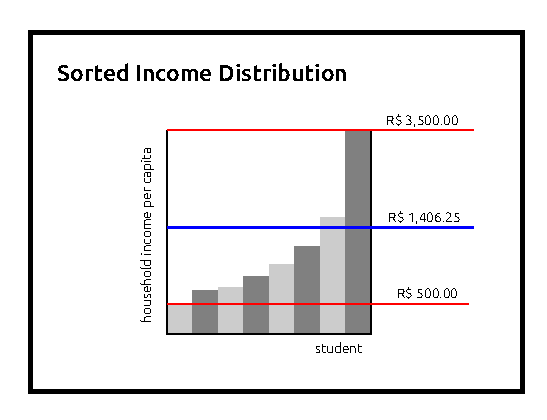
\includegraphics[width=0.9\textwidth]{images/chapter-06/income-example.pdf}}

\par\medskip\ABNTEXfontereduzida\selectfont\textbf{Source:} Created by the author (2024).
\end{figure}

\begin{figure}[ht!]
\centering

\caption{\textmd{Chart of the Lorenz curve of Table \ref{tbl:classroom-dist} values. The red line marks the maximum percentage value. The blue line represents the ideal one.}}
\label{fig:lorenz-curve-example}
\fcolorbox{gray}{white}{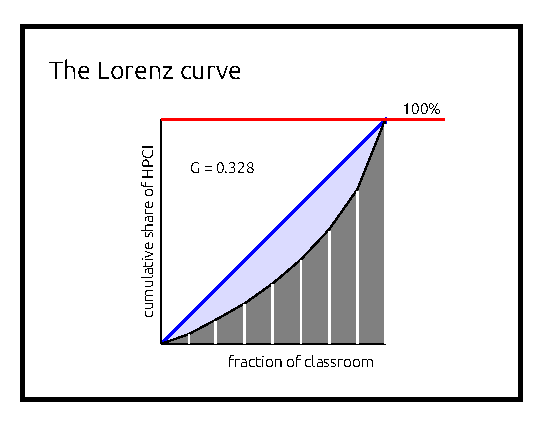
\includegraphics[width=0.9\textwidth]{images/chapter-06/lorenz-example.pdf}}

\par\medskip\ABNTEXfontereduzida\selectfont\textbf{Source:} Created by the author (2024).
\end{figure}

It is possible to see there is an inequality from Figure \ref{fig:income-example}. But if I need to compare this classroom inequality to inequalities of other people groups, it recommends normalizing all values. The Lorenz curve makes it through two steps: (i) using as normalizing reference the sum percentage of all resources (in this case, \gls{HPCI}), and (ii) working with the accumulated values of resources instead of the corresponding one of each individual. Figure \ref{fig:lorenz-curve-example} plots the Lorenz curve with the Table \ref{tbl:classroom-dist} values. 

An interesting possibility when we use the Lorenz curve is to compute the \gls{GI} \cite{farris:2010}. In this example, the \gls{GI} is 0.328\footnote{Thanks to Buck Shlegeris for opening her JavaScript code to compute Gini Index at \url{https://github. com/bshlgrs/economics-demos}.} (see Figure \ref{fig:lorenz-curve-example}). The closer \gls{GI} is to zero, the greater the equality of a given group. Otherwise, the closer \gls{GI} is to one, the greater the inequality of a given group. The \gls{GI} of the blue line of Figure 6.2 is zero, representing the equality reference concerning \gls{HPCI}.

According to the World Bank\footnote{Available in \url{https://data.worldbank.org/indicator/SI.POV.GINI?locations=BR}.}, Brazil's and Finland's \gls{GI} were 0.489 and 0.277, respectively. Thus, this hypothetical classroom is less unequal than Brazil but more unequal than Finland. Although social inequality is a complex and multifactorial problem, \gls{GI} signals as a first indicator to situate income inequality in a broader context.

The idea in relation to the sampling strategy was to focus on the 1st and 4th quartiles (\acrshort{Q}1 and \acrshort{Q}4) of the classroom income distribution, where \acrshort{Q}1 represents the lowest socioeconomic student group and \acrshort{Q}4 represents the highest group (see Figure \ref{fig:sampling-classes}). I will describe how I use these groups for choosing students during data collection in Section \ref{res-des-sec:phd-route}.

\begin{figure}[ht!]
\centering

\caption{\textmd{Chart representing the sampling classes from Lorenz curve of a classroom. \acrshort{Q}1, \acrshort{Q}2, \acrshort{Q}3, and \acrshort{Q}4 are the quartiles of the classroom HPCI distribution, where \acrshort{Q}1 represents the lowest socioeconomic student group and \acrshort{Q}4 represents the highest group.}}
\label{fig:sampling-classes}
\fcolorbox{gray}{white}{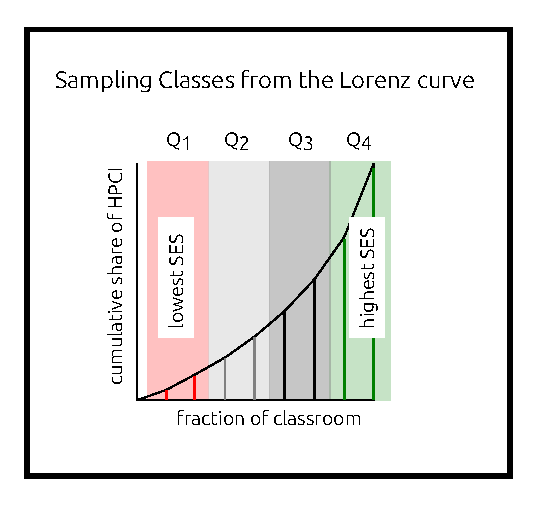
\includegraphics[width=0.9\textwidth]{images/chapter-06/sampling-classes.pdf}}

\par\medskip\ABNTEXfontereduzida\selectfont\textbf{Source:} Created by the author (2024).
\end{figure}
\section{Data Analysis}
\label{res-met:data-analysis}

The data analysis consisted primarily of building results from each data source using a best-effort approach (considering a trade-off of constraints like time and people availability), aiming to triangulate them in a future step. For interviews, I adopted the descriptive coding as presented by \citeonline[p.~4]{saldana:2013}. For questionnaires, I made charts (e.g., Lorenz Curve) and considered non-quantitative data to help identify potential samples. For the document survey, I aggregated the available data (mainly in public sheets). Lastly, for observational notes, I concentrated my efforts on adjusting my researcher's view concerning the concrete phenomenon in this class, desiring to "get a feeling" about strategic research decisions.

Frame \ref{frame:research-methodology} summarizes some methodological choices in this chapter.



%a diferença do quadro pra tabela é que o quadro tem linhas verticais
\begin{quadro}[!htb]
\caption{Main research methodological choices.}
\label{frame:research-methodology}
\centering
\begin{tabular}{|l|l|}
\cline{1-2}

\textbf{Approach} & 
Qualitative (Predominantly) \\

\textbf{Epistemological Perspective} &
Interpretive (Predominantly)\\

\textbf{Sampling Strategy} &
Comparison-focused (Intensity)\\

\textbf{Data Collection Technique} &
Descriptive Coding \\
\hline

%A& B &  C& D &E  \\ \cline{1-5}
%\multirow{3}{*}{1}  & 2 &  3& 4& 5 \\
% &  2 &  3& 4& 5  \\
% &  2 &  3& 4& 5 \\
% \cline{1-5}
\end{tabular}
  \par\medskip\ABNTEXfontereduzida\selectfont\textbf{Source:} Created by the author (2024). \par\medskip
\end{quadro}

% \fbox{
%     \begin{minipage}[htb]{0.9\textwidth}
%         \vspace{0.3cm}
                
%         \colorbox{gray!30}{% create a colored box
%             \makebox[0.975\textwidth][l]{% center the text on the page
%                 \ \ \textbf{Further Writing}
%             }
%         }

%         \vspace{0.1cm}
        
%         \begin{itemize}
%             \item Describing what are coding techniques according Merriam and Tisdell ("Qualitative Data Analysis" chapter).
%         \end{itemize}

%         \vspace{0.25cm}
        
%     \end{minipage}
% }
  
\chapter{Research Design}
\label{chap:res-design}

 Once I carried out the discussion about the research methodology, more specific steps needed to be defined. Research design informs us in more detail about all methods or techniques used for conducting research. In this moment, I describe the instantiation of context, sampling, and other essential information for research decision-making. 
 
I arrange the remainder of the chapter as follows. Section \ref{res-des-sec:context} presents the research context where I conducted the research. Section \ref{res-des-sec:active-learning} delineates the active learning context where this research is immersed. At last, Section \ref{res-des-sec:phd-route} details my \gls{Ph.D.} route, describing the main phases of the research walking.

\section{Research Context}
\label{res-des-sec:context}

The research context was an undergraduate \gls{IS} program in Recife, Brazil. This program is conducted at \gls{CIn} of the \acrfull{UFPE}. In the fourth semester, a \acrfull{PBL} approach integrates three courses of this program (Figure \ref{fig:pbl-group}): \gls{MIS}, \gls{PPM}, and \gls{BPM}. As mentioned in Section \ref{sdl-relations-ss:pbl}, \gls{PBL} has \acrfull{SDL} as a crucial element. \gls{NEXT} Research Group has a long experience in the adoption of \gls{PBL} in \acrfull{CEd} \cite{santos:2021}, favoring to investigate \gls{SDL} construct in a structured and solid computing learning space, being responsible for implementing \gls{PBL} in this \gls{IS} program.

\begin{figure}[ht!]
\centering

\caption{\textmd{Illustration of the integrated \acrshort{PBL} approach composed of three courses. I use an estimator for \acrfull{SES} to help to pick students to follow up closer.}}
\label{fig:pbl-group}
\fcolorbox{gray}{white}{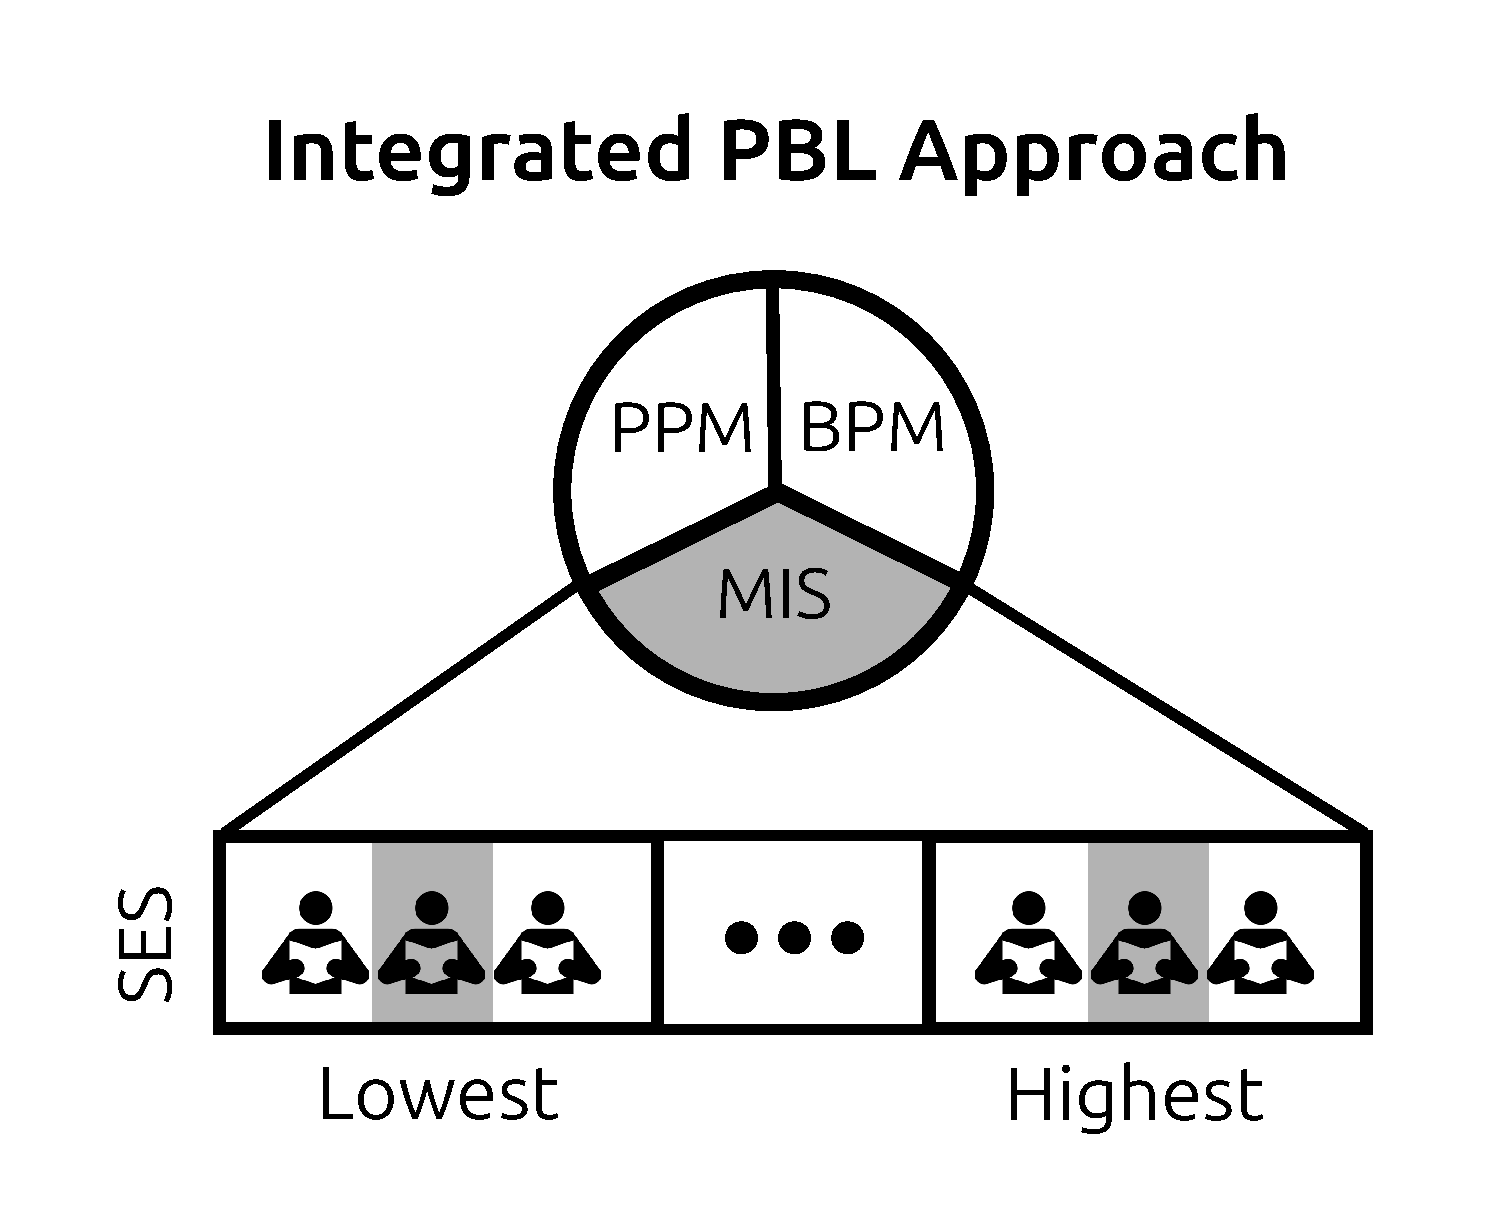
\includegraphics[width=0.9\textwidth]{images/chapter-07/pbl-group.pdf}}

\par\medskip\ABNTEXfontereduzida\selectfont\textbf{Source:} Created by the author (2024).
\end{figure}

This research concentrated more efforts on \gls{MIS} course during the data collection step. My advisor was responsible for facilitating this course in the 2023.1 academic term.

It is essential to highlight that all federal teaching institutions in Brazil adopt affirmative actions for student entry into higher education. As explained in Section \ref{equity-sec:br-context}, these affirmative actions consider various aspects, emphasizing if students attended their whole high school in public teaching institutions. Thus, it should be possible to see significant functioning differences (Section \ref{sen-ss:functioning}) among the students even after four terms of this program.

% \vspace{0.3cm}
% \fbox{
%     \begin{minipage}[htb]{0.9\textwidth}
%         \vspace{0.3cm}
                
%         \colorbox{gray!30}{% create a colored box
%             \makebox[0.975\textwidth][l]{% center the text on the page
%                 \ \ \textbf{Further Writing}
%             }
%         }

%         \vspace{0.1cm}
        
%         \begin{itemize}
%             \item Describing the PBL Framework  \cite{rodrigues:2016}.
%         \end{itemize}

%         \vspace{0.25cm}
        
%     \end{minipage}
% }
\section{Active Learning Context}
\label{res-des-sec:active-learning}

As presented before (Section \ref{sdl-sec:relations}), \gls{SDL} establishes relations with many active learning approaches. In this section, I present the active learning context in which the \gls{SDL} construct was investigated in this research. I detail the \gls{PBL} adopted in this research context (Section \ref{res-des-sec:context}), delineating the \gls{PBL} By-Cycles Framework \cite{alexandre:2018} from four essential steps in this evolution journey (in order of arising): (i) \gls{PBL}-Test, (ii) \gls{xPBL}, (iii) \gls{PBL} Framework, and (iv) \gls{PBL-SEE}.

The first important step of \gls{NEXT} aiming to structure the learning processes in \gls{PBL} for \gls{CEd} was the \gls{PBL}-Test \cite{santos:2013}. \gls{PBL}-Test is a model to evaluate the maturity of
teaching processes in a \gls{PBL} approach. The idea is to verify the perception of all \gls{PBL} stakeholders (e.g., facilitators, tutors, students) concerning \gls{PBL} principles (as presented in Section \ref{sdl-relations-ss:pbl}). One of the main results after the \gls{PBL}-Test application is to locate what level of maturity your \gls{PBL} is (that can be: insufficient, initial, satisfactory, good, or excellent level).

The second step in the \gls{NEXT} evolution was the proposal of the \gls{xPBL} \cite{santos:2014}. \gls{xPBL} is a methodology for managing \gls{PBL} when teaching Computing. The idea is to provide an alternative to yPBL methodology \cite{exposito:2010}, providing a relationship between \gls{PBL} principles and five methodology elements (obtained from previous \gls{NEXT} research experiences). These key methodology elements are (i) problem, (ii) environment, (iii) content, (iv) human capital, and (v) process. The authors presented, for each element, a pathway to conduct a 5W2H technique \cite{klock:2016} aiming to help computing educators in a \gls{PBL} course design.

The third \gls{NEXT} step was the proposal of the \gls{PBL} Framework \cite{rodrigues:2016}. The framework idea is to ensure satisfactory results by using \gls{PBL} in \gls{CEd}, reusing as a base the Deming cycle: \gls{PDCA} \cite{dudin:2015}. \gls{PBL} Framework incorporates both \gls{xPBL} (Plan Phase) and \gls{PBL}-Test (Act Phase), also signaling an authentic assessment as one of its key components (Check Phase).

The last step in this evolution was an authentic assessment model for
\gls{PBL}-Based Software Engineering Education: \gls{PBL-SEE} \cite{santos:2016}. \gls{PBL-SEE} address the Check Phase of \gls{PBL} Framework with a structured model, being composed of three levels (i) student assessment, (ii) \gls{PBL} evaluation, and (iii) teaching assessment. The objective of this model is to indicate assessment strategies that guarantee the effectiveness of the \gls{PBL} approach throughout its management cycle. Educational Objectives are established based on \gls{RBT}, associating each verb in \gls{RBT} six levels to \gls{xPBL} five elements. 

Figure \ref{fig:pbl-by-cycles} presents the schema of \gls{PBL} By-Cycles Framework with the main steps detailed here.
\section{Ph.D. Route}
\label{res-des-sec:phd-route}

A good way to present the methodological route of this research project is by knowing my Ph.D. route. I divide my Ph.D. study into three phases, describing the project structuring (Section \ref{phd-route-ss:proj-str}), the pre- and in-intervention (Section \ref{phd-route-ss:pre-int} and \ref{phd-route-ss:in-int}), and the analysis and discussion (Section \ref{phd-route-ss:ana-dis}). I scheme this route in Figure \ref{fig:phd-route}.

\begin{figure}[ht!]
\centering

\caption{\textmd{Schema of \acrshort{PBL} By-Cycles Framework using the Deming cycle (\acrshort{PDCA}) structure.}}
\label{fig:pbl-by-cycles}
\fcolorbox{gray}{white}{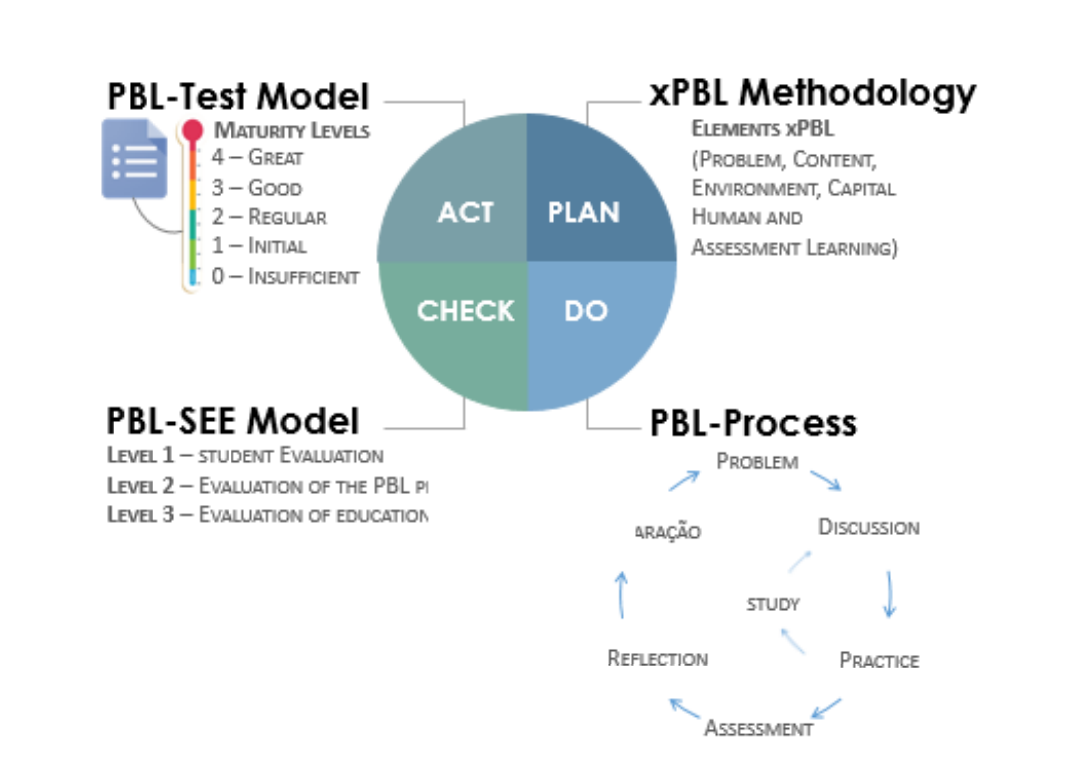
\includegraphics[width=0.9\textwidth]{images/chapter-07/pbl-by-cycles.png}}

\par\medskip\ABNTEXfontereduzida\selectfont\textbf{Source:} \citeonline[p.~60]{alexandre:2018}.
\end{figure}

\begin{figure}[ht!]
\centering

\caption{\textmd{Schema presenting my \acrshort{Ph.D.} route composed of three big phases: (i) project structuring, (ii) pre- and in-intervention, and (iii) analysis \& discussion.}}
\label{fig:phd-route}
\fcolorbox{gray}{white}{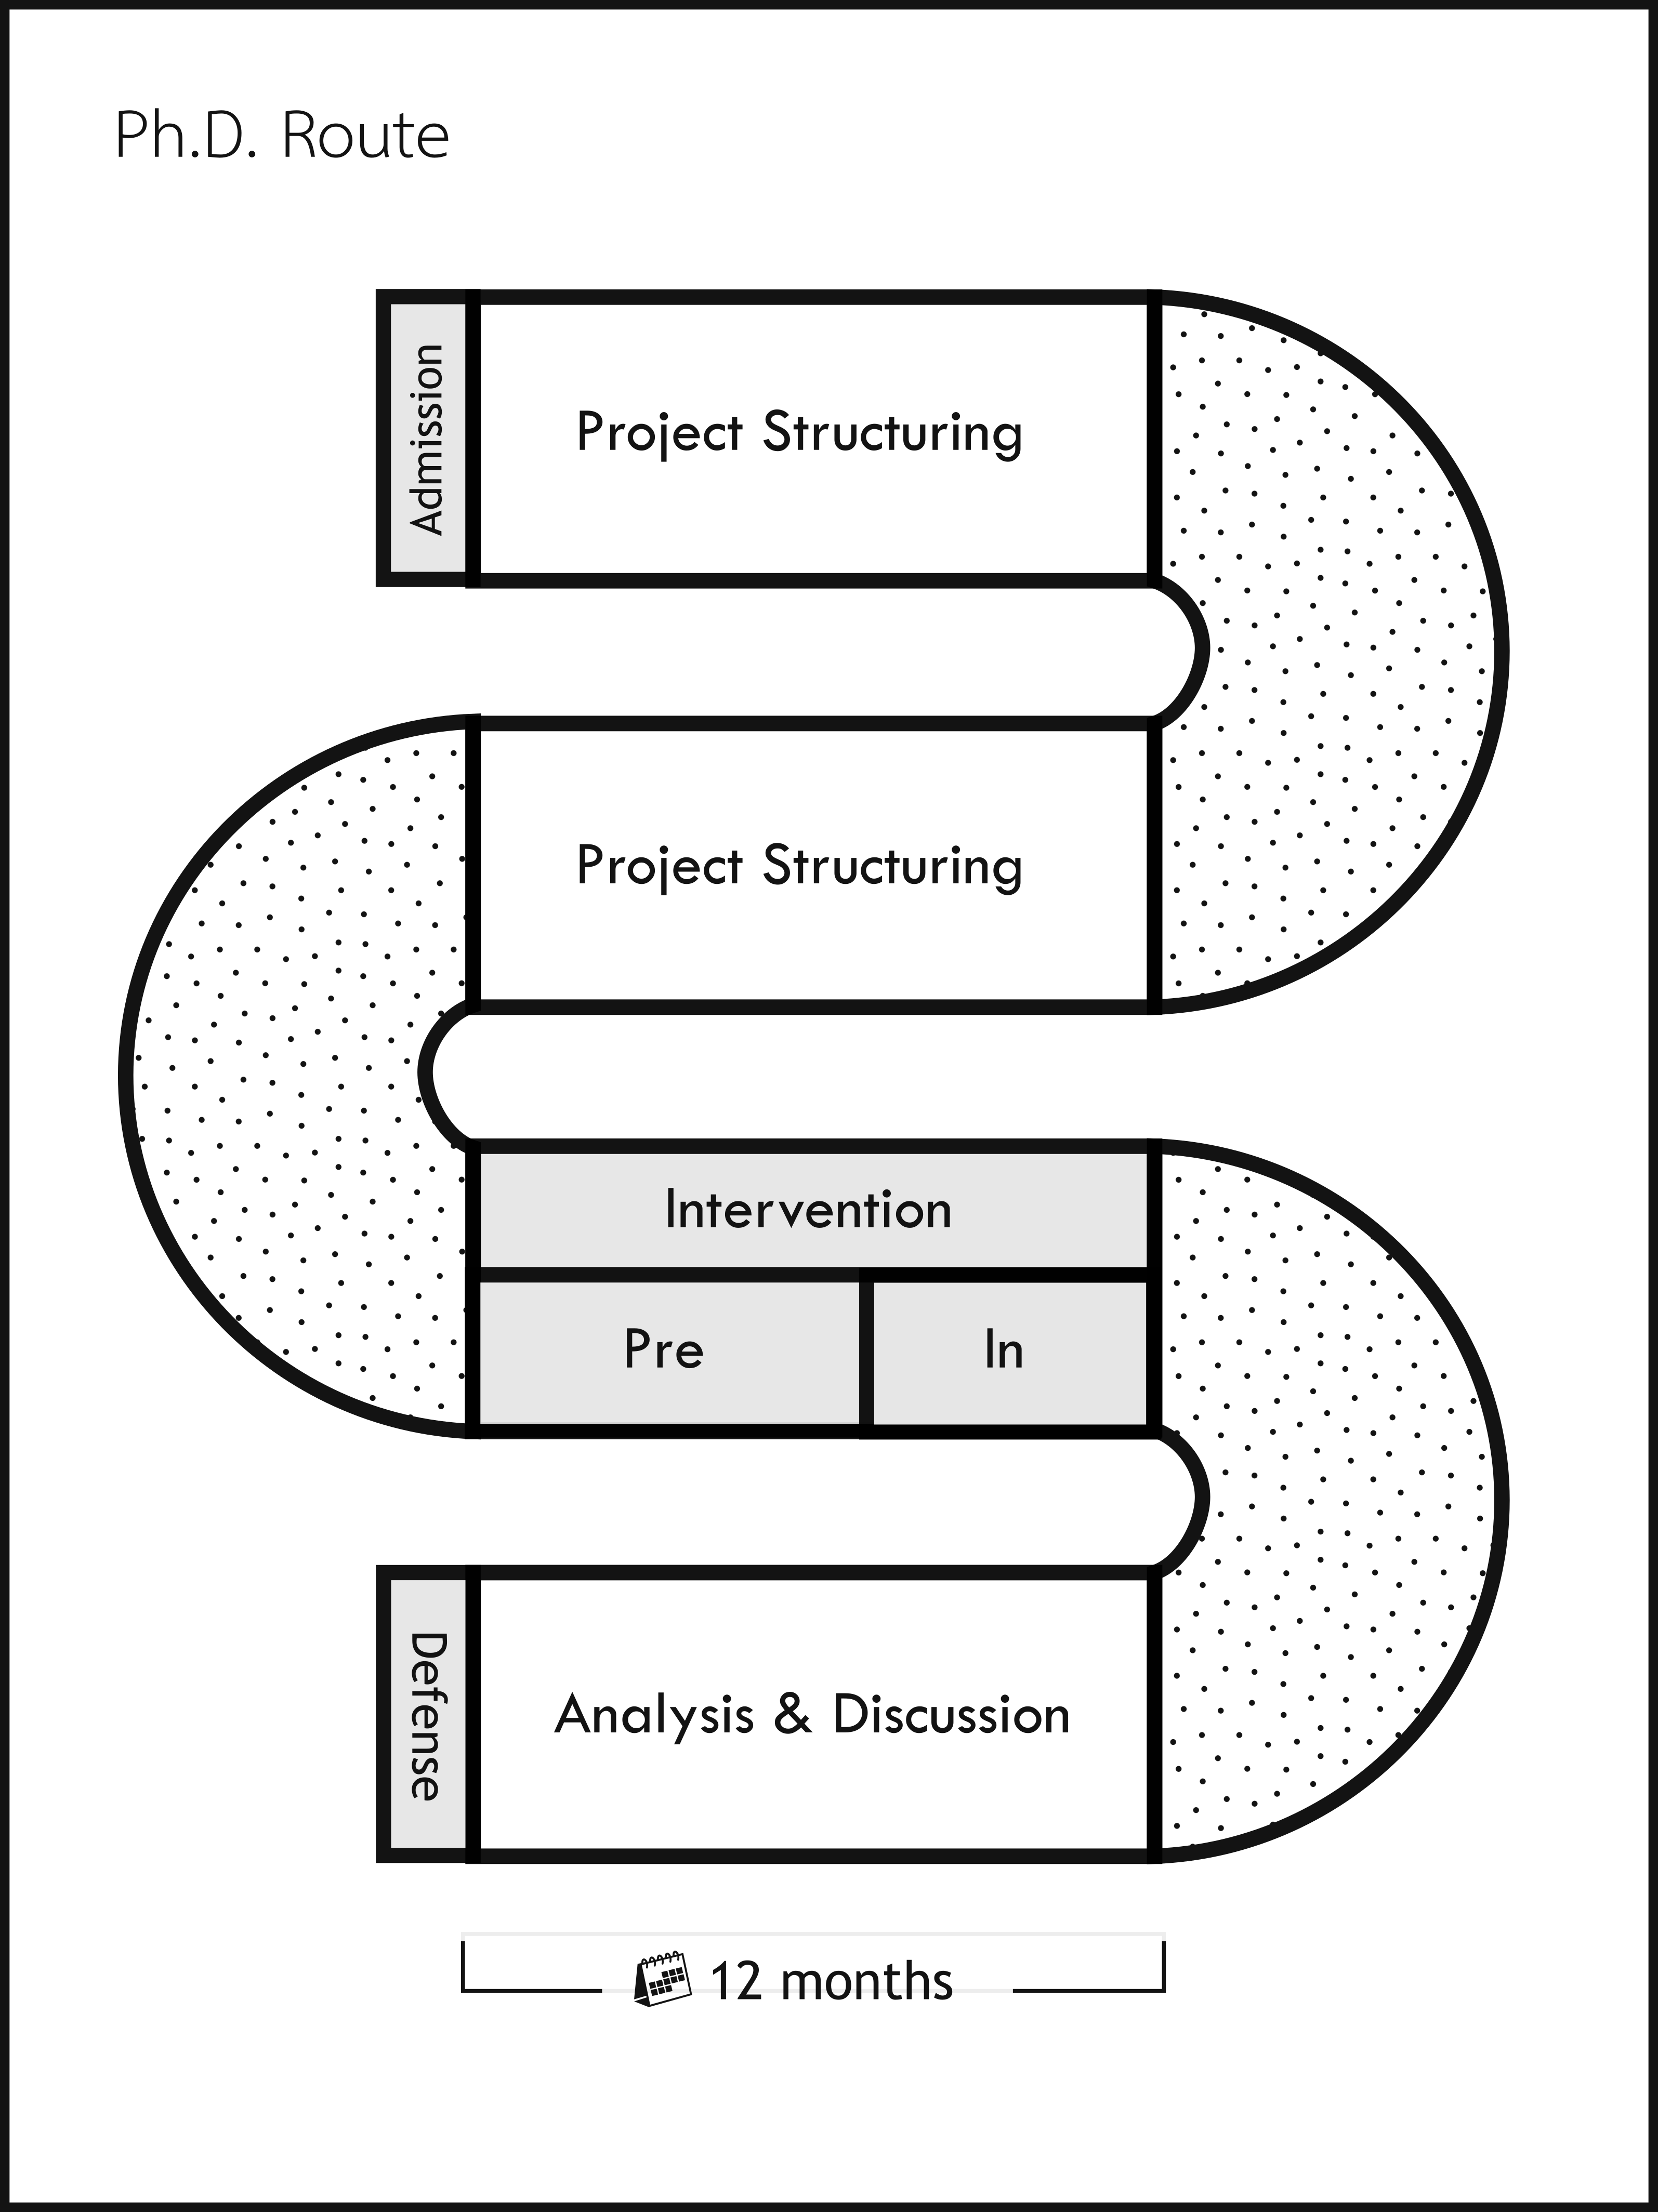
\includegraphics[width=0.9\textwidth]{images/chapter-07/phd-route.png}}

\par\medskip\ABNTEXfontereduzida\selectfont\textbf{Source:} Created by the author (2024).
\end{figure}

\subsection{Project Structuring}
\label{phd-route-ss:proj-str}

The first phase covers all activities and decisions responsible for helping structure the research project. This phase lasted nearly 24 months, comprehending from my admission to the \gls{Ph.D.} program (October 2020) until the qualifying exam (November 2022). I list the main activities that are: attended courses, reading tasks, tutoring, paper writing, and qualifying project. I will describe each of them in detail as follows.

My advisor and I decided on a set of introductory courses that would help me in this phase. The major part was related to research methodology: (i) “Research in Computing Science”, (ii) “Evidence-based Software Engineering”, and (iii) “Qualitative Research in Software Engineering”. I attended all of them at \gls{CIn}. Beyond these, a strategic course was “Education and Society” that I had the opportunity to attend at the \gls{UFPE} Education Center. These four courses gave me incredible constructs to structure Chapters \ref{chap:rel-work}, \ref{chap:reflex-essay}, and \ref{chap:res-methodology} of this research.

Another crucial activity during this phase was my readings. Although part of my academic journey as a professor provided me with previous knowledge about active learning in \acrfull{CSE} area, I needed to deepen my research about \gls{SDL} and equity concepts. This activity pervaded the whole project structuring (and part of other \gls{Ph.D.} route phases), having the Chapters \ref{chap:intro}, \ref{chap:sdl}, and \ref{chap:equity} as the more visible results.

Bearing to know the potential field of data collection, I helped my advisor (and my colleague-tutors) during the integrated \gls{PBL} approach (Section \ref{res-des-sec:context}) as a tutor during the 2020.2 academic term (from May to September 2021). This opportunity allowed me to understand the \gls{PBL} By-Cycles Framework \cite{alexandre:2018} in more detail, observing all the possibilities to intersect my research interests into a context in which the \gls{PBL} in \gls{CSE} achieved a high level of maturity \cite{santos:2013}. The first outline of the research design arose during these tutoring moments.

Not all doctoral credits are offered as courses in a classical format. A part of them can be conducted through individual mentoring between an advisor and doctoral candidate on a specific topic during an academic semester. In these moments, I could deepen some strategic discussions related to my research by writing about \gls{PBL} diagnosis \cite{santos:2022}, research ethics \cite{bispojr:2021-wei}, and neutrality \cite{bispojr:2022-educomp}. A narrative describing the whole walking of paper writings during my \gls{Ph.D.} is available in Appendix \ref{chap:appendix-a}.

Last but not least, I wrote my qualifying project. Writing, as 
\citeonline{booth:2008-craft} assert, is not only a final result of a cycle but also a way of thinking. The several writing cycles forced me to put my initial ideas on paper, allowing me to refine and achieve a satisfactory version. I received valuable feedback from the examining committee, giving me essential elements to improve my research project and better structure my data collection.

\subsection{Pre-Intervention}
\label{phd-route-ss:pre-int}

The first part of the second phase covers all preparatory activities to follow up the \gls{SDL} trajectories of CSE students \textit{in situ} and remotely. This phase lasted nearly seven months, ranging from my qualifying exam (November 2022) until the first meeting with the integrated \gls{PBL} class (May 2023). I list the main activities that are: ethical committee application, document survey, initial observing, first meeting, and socioeconomic questionnaire application.  I will describe each of them in detail as follows.

After the qualifying exam, my advisor and I considered all the contributions from the examining committee and structured the final project to apply for the \gls{IRB}. Because I collected all data from human subjects in a Brazilian institution, I translated this project into Portuguese before the submission. The first project submission for the \gls{UFPE} \gls{IRB} occurred on March 20, 2023. The sending of the first \gls{IRB} decision happened on May 03, 2023, asking to do a minor review. I re-submitted the revised project on May 04, 2023. Lastly, the \gls{IRB} manifested their final decision on May 10, 2023, approving this research project, generating the  \gls{CAAE}\footnote{CAAE is the certificate of presentation for ethical appreciation that allows us to verify the approval status of research projects on Brazilian \gls{IRB}s on a national website called \textit{Plataforma Brasil}(\url{https://plataformabrasil.saude.gov.br/}). The \gls{CAAE} number of this project is 68111823.3.0000.5208.}.

During the \gls{IRB} process of appraisal, I conducted part of the document survey. There are several open data sources, like \textit{Portal de Dados Abertos} (\gls{UFPE})\footnote{Available in \url{https://dados.ufpe.br/}.} and \textit{Portal Brasileiro de Dados Abertos}\footnote{Available in \url{https://dados.gov.br/organization/universidade-federal-de-pernambuco}.}. I obtained aggregated data concerning \gls{UFPE} \gls{IS} program, focusing my attention on enrolled undergraduates of the 2023.1 term (see Section \ref{results-ss:classroom-data}). The political pedagogical project of the program and the education plans of each course of the integrated \gls{PBL} class were obtained and are available on the public repository of this \gls{Ph.D.} study\footnote{See \url{https://github.com/bispojr/phd-info}.}. 

%{\color{red} Once the \gls{IRB} provided the project approval, the data collection involving human subjects was conducted. At that moment, I requested two academic documents of each student of the integrated \gls{PBL} classroom from the responsible sector of the program: (i) current educational history, and (ii) latest socioeconomic data. My idea was to get any potential data liable to triangulate to interviews, observation notes, etc.}

It made part of the planning phase a previous preparation period of the integrated \gls{PBL} approach. This period usually occurs before each conduction of the PBL integrated approach, gathering all professors, tutors, and clients to adjust dates and activities, guaranteeing an appropriate integration among the three courses. After I collected their consent and assent, I observed these meeting activities. They created educational artifacts to manage student activities in the \gls{LMS} and private spreadsheets (or docs). I obtained reading-only access to the responsible for these artifacts too. Figure \ref{fig:methodological-route} illustrates the whole intervention phase schematically. 

\begin{figure}[ht!]
\centering

\caption{\textmd{Illustration of the methodological route of part of this research project. A timeline with the two data collection phases (pre- and in-intervention) is presented, situating the data collection instruments along with it, according to their time granularity.}}
\label{fig:methodological-route}
\fcolorbox{gray}{white}{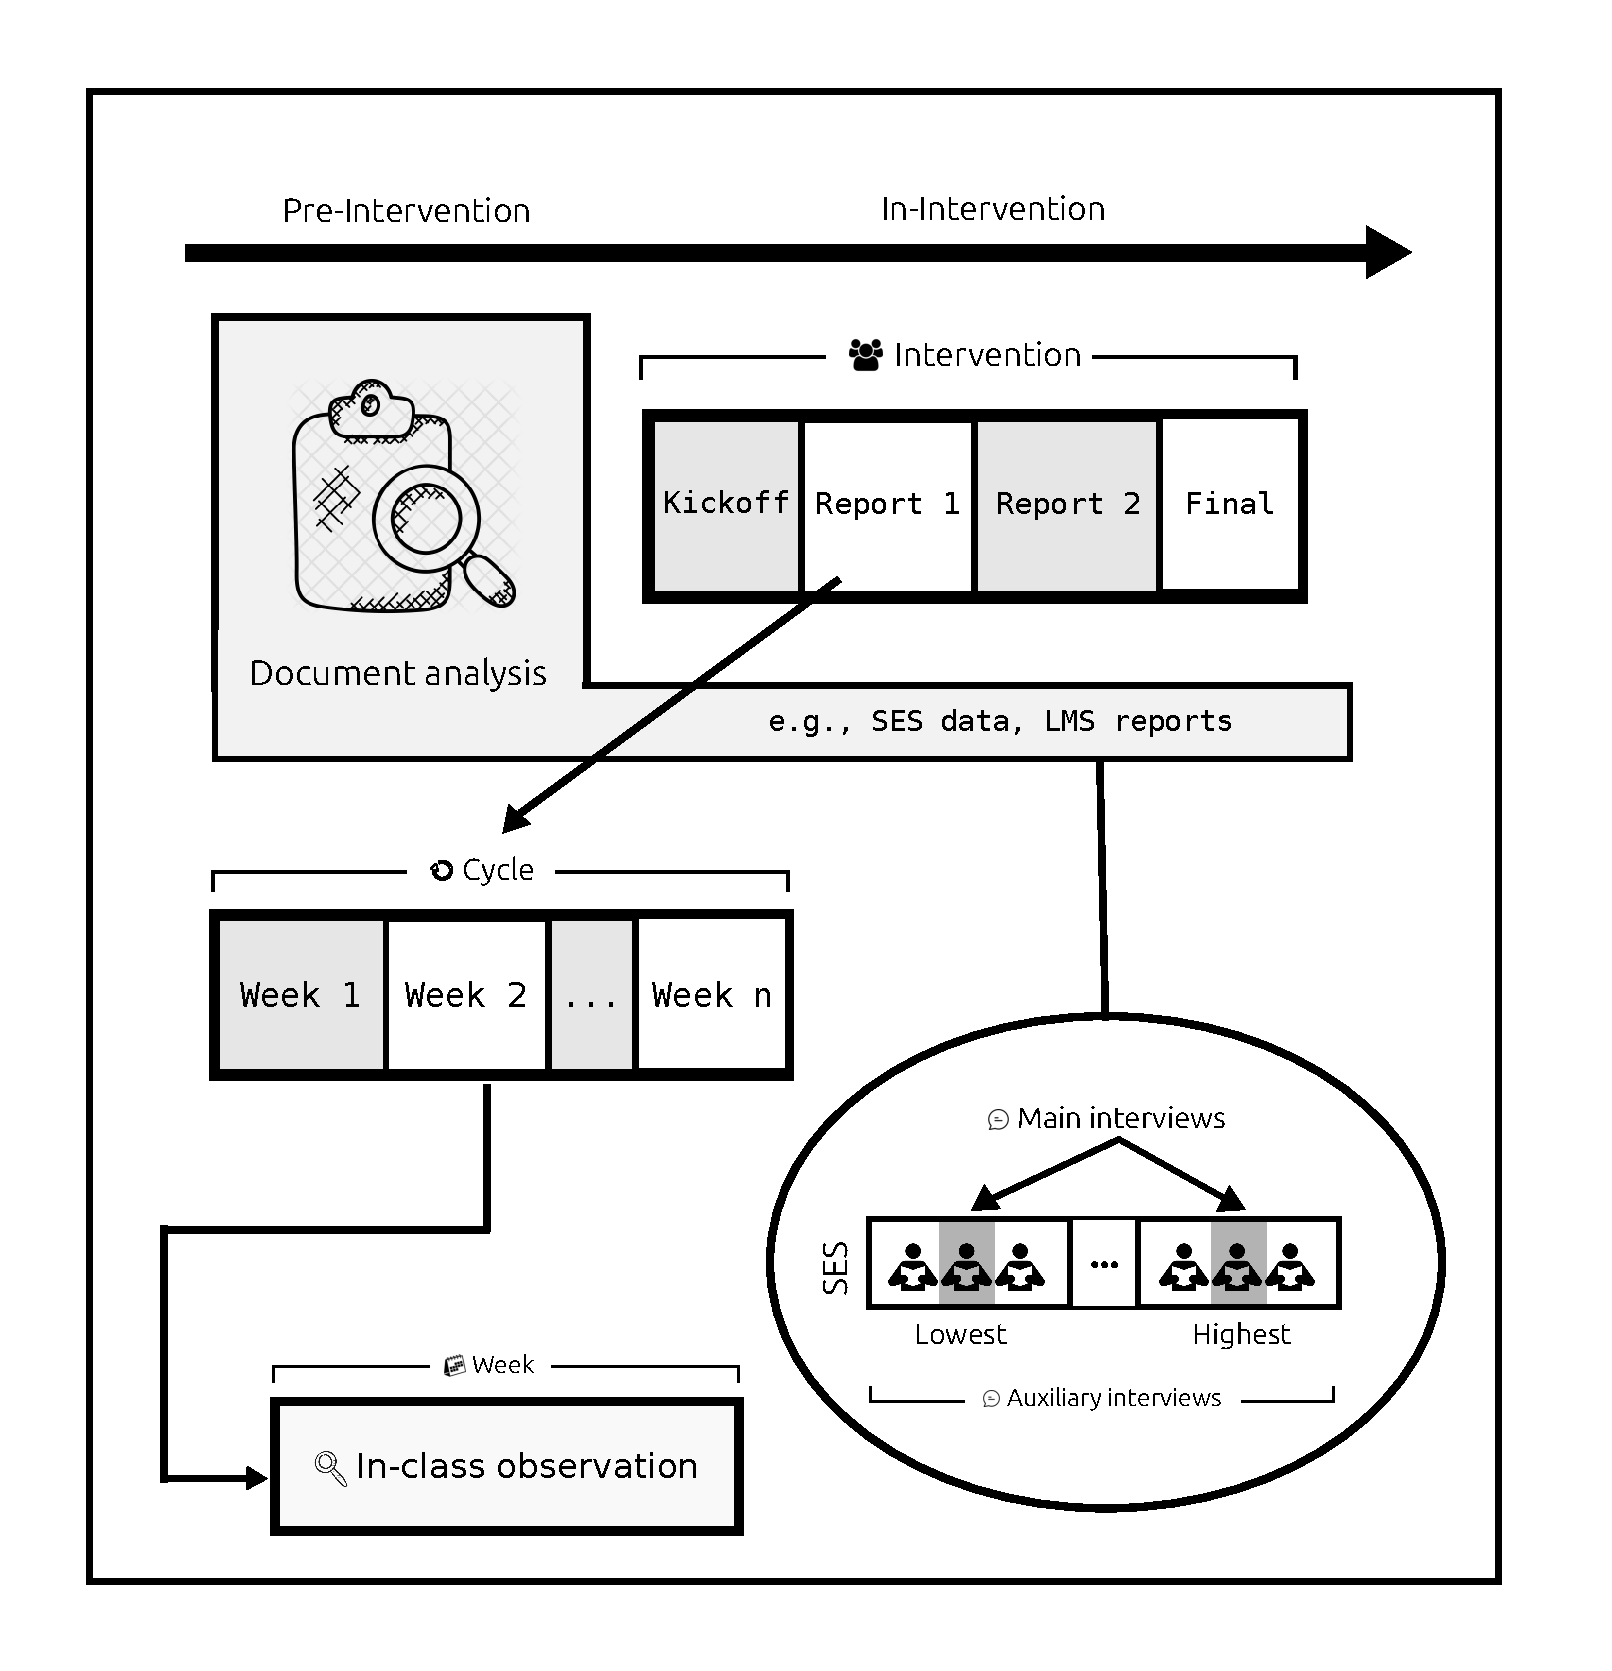
\includegraphics[width=0.9\textwidth]{images/chapter-07/new-methodology.pdf}}

\par\medskip\ABNTEXfontereduzida\selectfont\textbf{Source:} Created by the author (2024).
\end{figure}

As part of the consent and assent process, I presented my research project on May 30, 2023, during the first \gls{MIS} class. This presentation title was "Human Aspects in MIS"\footnote{Originally, "\textit{Aspectos Humanos em SGE}" in Brazilian Portuguese.}, lasting 40 minutes. The presentation comprised the following four topics: (i) introduction, (ii) notions on equity and ethics, (iii) research presentation, and (iv) consent for research\footnote{The presentation slides (in Brazilian Portuguese) are available on this \gls{Ph.D.} public repository: \url{https://github.com/bispojr/phd-info}.}. In the last topic, I avoided technical terms and concepts, focusing on showing the essence of research and all adopted care concerning research ethics involving humans, including current legal requirements \cite{bispojr:2021-wei}. I provided the informed consent form (and all ways to contact me during the research, in case of participation) for each student before this class (both on \gls{LMS} and repository). I kept the agreement of each student to participate in the research, counting on only those who answered me positively.

For students who voluntarily participated in the research (30 of 35 $\cong$ 85.71\% of \gls{MIS} class), I asked them to fill out a socioeconomic questionnaire (see Appendix \ref{chap:socio-quest}). This form allowed me to get socioeconomic information and plot the Lorenz curve from the average \acrfull{HPCI} data. This curve helped me to estimate the \gls{SES} of the class, stratifying them into four classes. Thus, all students belonged to a class alongside a continuum axis ranging between lower and higher \gls{SES} (see Section \ref{res-meth-ss:lorenz} and \ref{results-ss:classroom-data}). The idea was to pick two students and investigate these two ones during the term. I preferred to pick two students from the lowest and highest SES classes, respectively, aiming to understand if income disparity can be reflected in their capabilities. Another data source came from their classmates and other stakeholders, serving to triangulate and enrich the understanding of the research findings. Figure \ref{fig:participation-venn} presents in more detail the effective research participation of students in terms of \gls{ICF}, \gls{SQ}, and \gls{IP}.

\begin{figure}[ht!]
\centering

\caption{\textmd{Venn Diagram of the relations of three groups of students: those that (i) agreed with the \acrfull{ICF}, (ii) answered \acrfull{SQ}, and (iii) participated in interviews (\acrshort{IP}).}}
\label{fig:participation-venn}
\fcolorbox{gray}{white}{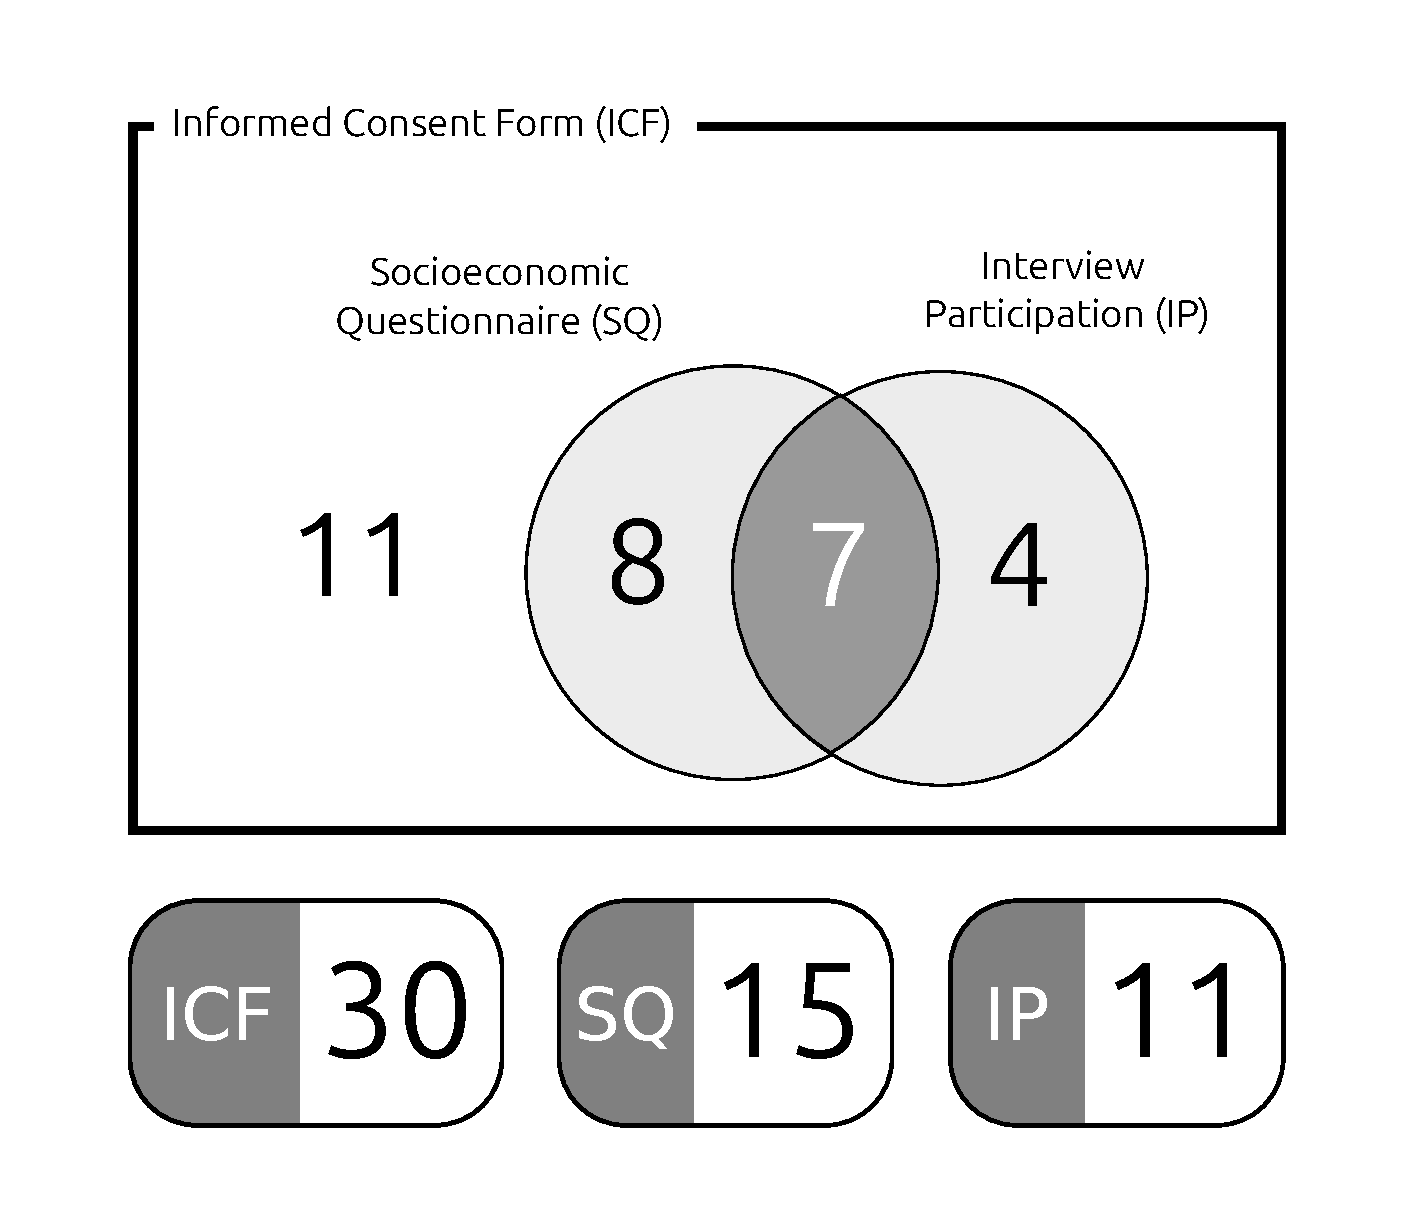
\includegraphics[width=0.9\textwidth]{images/chapter-07/participation.pdf}}

\par\medskip\ABNTEXfontereduzida\selectfont\textbf{Source:} Created by the author (2024).%\citeauthor{manualufpe2020} (\citeyear{manualufpe2020}) \par\medskip
\end{figure}

% \fbox{
%     \begin{minipage}[htb]{0.9\textwidth}
%         \vspace{0.3cm}
                
%         \colorbox{gray!30}{% create a colored box
%             \makebox[0.975\textwidth][l]{% center the text on the page
%                 \ \ \textbf{Further Writing}
%             }
%         }

%         \vspace{0.1cm}
        
%         \begin{itemize}
%             \item Describing first meeting (PBL planning).
%             \item Describing the research presentation (first day of class).
%             \item Describing the acceptance to participate in research, and interviews (included informed consent).
%             \item Creating a list of the date of interviews through a timeline term.
%         \end{itemize}

%         \vspace{0.25cm}
        
%     \end{minipage}
% }


\subsection{In-Intervention}
\label{phd-route-ss:in-int}

The second part of the second phase covers all effective activities to follow up the \gls{SDL} trajectories of \gls{CSE} students \textit{in situ} and remotely. This phase lasted five months, comprehending from the first (May 2023) to the last meeting with the integrated \gls{PBL} class (October 2023). I list the main activities that are: interviews, observation, and documental analysis. Figure \ref{fig:methodological-route} illustrates the whole intervention phase schematically. 

The interviews were the most important means of data collection. I conducted three blocks of interviews (in a total of 11 different interviewees): the first one composed of three interviews (happening inside of Kickoff cycle), the second one composed of seven interviews (happening inside of Status Report 1 cycle), and the third one composed of a single interview (happening after the Final Report, see Table \ref{tbl:interview-dates}). The size of each block is different among themselves due to two reasons: (i) first, I conducted these interviews based on availability of each student (bearing in mind that this \gls{IS} program occurs at the night shift), and (ii) second, I opted to concentrate the most of interviews until the end of July 2023 because between August 2023 and January 2024 I was at Brunel University London in \gls{UK}, performing the Analysis \& Discussion phase also together to my co-advisor Prof. Marcus Vinicius De Matos (and I tried to offer the possibility for the interviewed could choose a in-person or remote format). Aiming to preserve the identity of each \gls{RP}, I use an alias like \gls{RP}4 to represent any research participant, and the aliases Chavo and Quico\footnote{Chavo and Quico are characters of Chespirito, a Mexican sitcom written by Roberto Bolaños. Chavo is the main character of Chespirito, a homeless person who sleeps inside a barrel. Quico is the son of Doña Florinda and a late naval captain. Chespirito presents him as a spoiled and overprotected 9-year-old-boy.} to represent the chosen participants from the lowest and highest \gls{SES} student groups (\gls{Q}1 and \gls{Q}4), respectively. I interviewed Chavo in the first block remotely, and Quico in the second block in-person. The semi-structured interview script is available in Appendix \ref{chap:appendix-scripts}.

\begin{table}[htb]
\caption{List of the three blocks of interviews indicating the period, \acrshort{PBL} cycle, and research participants.}
\label{tbl:interview-dates}
\centering
\rowcolors{1}{}{lightgray}
\begin{tabular}{
    m{3cm}|
    m{4cm}|
    m{4cm}|
    m{4cm}
}
    \hline
    \multicolumn{1}{c|}{
        \textbf{Block} 
    } &
    \multicolumn{1}{c|}{
    \textbf{Participants}
    } &
    \multicolumn{1}{c|}{
    \textbf{Period}
    } &
    \multicolumn{1}{c}{
    \textbf{Cycle}
    } \\
    
    \hline
    \multicolumn{1}{c|}{
        1
    } &
    \multicolumn{1}{c|}{
        RP1-2, Chavo
    } &
    \multicolumn{1}{c|}{
        May 30 to Jun 22
    } &
    \multicolumn{1}{c}{
        Kickoff
    } \\

    \multicolumn{1}{c|}{
        2
    } &
    \multicolumn{1}{c|}{
        RP3-8, Quico
    } &
    \multicolumn{1}{c|}{
        Jun 23 to Jul 25
    } &
    \multicolumn{1}{c}{
        Status Report 1
    } \\

    \multicolumn{1}{c|}{
        3
    } &
    \multicolumn{1}{c|}{
        RP9
    } &
    \multicolumn{1}{c|}{
        After Sep 21
    } &
    \multicolumn{1}{c}{
        After Final Report
    } \\
    \hline
    % \hline
    % \multicolumn{2}{c}{Item of Information} &
    % Related \gls{DSRQ}\\
    % \hline
    % Research &
    % Type & \gls{DSRQ}.1 \\
    % & Kind & \gls{DSRQ}.1 \\
    % & Methodology & \gls{DSRQ}.1 \\
    % \hline
    % Context &
    % Educational Level & \gls{DSRQ}.2 \\
    % & Country / Region & \gls{DSRQ}.2 \\
    % \hline
    % Equity & 
    % Equity Issue & \gls{DSRQ}.3 \\
    % & General Equity Theory / Framework & \gls{DSRQ}.3 \\
    % \hline
    % - &
    % Active Learning Approach & \gls{DSRQ}.4\\
    % \hline
    
\end{tabular}

\par\medskip\ABNTEXfontereduzida\selectfont\textbf{Source:} Created by the author (2024). \par\medskip

\end{table}

The observation was conducted during some collective activities in the class. In summary, these activities encompassed all classes of three courses and all integrated presentations in the final of each cycle (Kickoff, Status Reports 1 and 2, and Final Report), focusing my attention on \gls{MIS} course. I obtained access to all forums, both those with only student access and those with professors and tutors (who talked among them privately). I also took observation notes continuously. This observation data guided me in choosing what student in each group I should prioritize to interview, for instance. Other different data sources could contribute to reinforcing the confluence of a finding or even significantly contrasting it, leading me to pay attention to certain aspects that previously were unconsidered. 

The documental analysis also was important over the intervention phase. During the integrated \gls{PBL} course, students made several documents in groups or individually. Some of these were deliverable artifacts required to be submitted in \gls{LMS} (or done in-person) at each cycle ending (e.g., \gls{UML} diagrams, slides, reports, exams). Other part consisted of form responses that each student helped the professors and tutors informing about the quality of the \gls{PBL} approach (e.g., \gls{PBL} tests, group and concept feedback). The data available from the open educational repositories and institutional databases were useful to situate the observed and reported conditions into a broader scenario both in \gls{UFPE} and in \gls{IS} class.%the institution and even the country.

%{\color{red} Lastly, I can trigger the focus group on specific occasions. In the cycle endings, a focus group can reveal key information about the capabilities that arise more naturally in a group setting instead of an individual one. Thus, the idea is to investigate capability aspects that emerge in a collective context. Furthermore, eventual mismatches can be identified between the individual and group perceptions. The semi-structured script of the focus group is available in  Appendix A3 (Table A3.2)}.


\subsection{Analysis \& Discussion}
\label{phd-route-ss:ana-dis}

The third (and last) phase covers all activities and decisions responsible for analyzing and discussing the research results. This phase lasted nearly 12 months, comprehending from the last meeting with the integrated \gls{PBL} class (October 2023) to the submission of this \gls{Ph.D.} thesis for examining committee appreciation (October 2024). I list the main activities: guidelines structuring, interview coding, document organization, data aggregation, and thesis writing completion.

After the qualifying project presentation, I received a precious feedback in a question format: "What would it be the research relevance to \gls{CEd} practitioners?"\footnote{I presented the research relevance to \gls{CEd} practitioners in Section \ref{intro-sec:rel-computing}.}. This feedback led me to include \gls{RG}3 seeking recommending guidelines to (\gls{CSE}) educational stakeholders concerning how to consider effectively equity issues and active learning from the \acrfull{CA} lens. To be honest, a seed of these guidelines had been discussed for us previously (before the qualifying project presentation) problematizing the \gls{CEd} neutrality presupposition \cite{bispojr:2022-educomp}. When I realized that this essay was the first document of guidelines, thus the next steps were to structure how to discuss equity effectively in \gls{CEd} decision-making collective of teachers (including \gls{CSE} perspective too).

Before the opportunity to submit a Springer chapter proposal for a book of \gls{OLEE}, my advisors and I decided to expand the scope of these guidelines to Engineering Education, providing a set of guiding questions to orientate an initial equity analysis for an Engineering decision-making collective of professors \cite{bispojr:2024-online-lab}. Bearing in mind that \glspl{LLM} started to be included as a new challenge in several educational contexts, I participated in the \gls{NMP} Conference talking about \gls{CEd}, equity, and \glspl{LLM}. In a second moment, my advisors and I extended this presentation ideas providing constructs to analyze equity in a computing class from our new concept of \gls{LLM} divide using \gls{CA} lens \cite{bispojr:2024-nmp}. These two contributions were written during my academic visit to Brunel University London.

After choosing the participants Chavo and Quico, I performed their interview coding. I used the Notion platform\footnote{See in \url{http://www.notion.so}.} to manage the codes, putting the little blocks of transcript interviews in a table column and the codes in another one. I conducted three big coding rounds, having several iterations into each round: (i) first round to code the main \gls{SDL} constructs (Section \ref{res-sec:interviews}), (ii) second round to code from \gls{SDL} goals and \gls{SSDL} perspective (\gls{RG}1, see Section \ref{disc-sec:sdl-trajectories}), and (iii) third round to code from \gls{SDL} capabilities\footnote{\gls{SDL} capabilities is a new concept that I created to establish the meeting between \gls{SDL} and \gls{CA} constructs. See more in Section \ref{disc-sec:sdl-capabilities}.} (\gls{RG}2, see Section \ref{disc-sec:sdl-capabilities}). It is important to note that I had the opportunity to join as a member of \gls{HDCA}\footnote{See \gls{HDCA} website: \url{https://hd-ca.org/}.}, participating more specifically in \gls{HDCA} Education Thematic Group. I was mentored by Prof. Monica Kuwahara from \gls{UFABC} since March 2024 in \gls{HDCA} Early Career Researchers and Practitioners Network Mentorship Program 2023-24\footnote{See more detail in \url{https://hd-ca.org/thematic_group/early-career-researchers-practitioners-network}.}. She is also one of the \gls{HDCA}'s coordinators for the Regional Network of Latin America, helping me to understand better about the application of \gls{CA} constructs.

The document organization was an activity to collect and arrange all related documents that were relevant to enlighten the interview findings. I divided into three document groups: curricula, \gls{UFPE} open data, and \gls{IS} class records. I detail each one in Section \ref{res-sec:context-overview}.

The data aggregation occurred in a posterior moment in relation to the document organization aiming to create charts to visualize the overall picture from each level of analysis (e.g., \gls{PBL} team, class, program, university). For instance, I put in Appendix \ref{chap:pbl-see-charts} all charts extracted from five elements of \gls{PBL-SEE}, locating Chavo and Quico in their respective \gls{PBL} team or even in their whole \gls{IS} class. The underlying idea is to realize the overall context for both participants, trying to capture some collective determinants for each one of them.

Lastly, in this phase, I finished the thesis writing. To be sure, the thesis writing was a continuous activity that started from the early phases of my \gls{Ph.D.} route. A significant part of my thesis came from the qualifying project, introducing new theoretical insights, adjusting the methodological design, and, mainly, presenting (Chapter \ref{chap:results}) and discussing (Chapter \ref{chap:discussion}) the results.

Frame \ref{frame:research-design} summarizes some research design choices in this chapter.

%a diferença do quadro pra tabela é que o quadro tem linhas verticais
\begin{quadro}
\caption{Main research design choices.}
\label{frame:research-design}
\centering
\begin{tabular}{|l|l|}
\cline{1-2}

\textbf{Research Context} & 
Information System 2023.1, \gls{MIS} Course \\
\hline

\multirow{2}{*}{\textbf{Number of Interviews}} &
 Main Interviews (2)\\
 & Auxiliary Interviews (9)\\
 \hline
 \textbf{Active Learning Approach} &
 PBL By-Cycles Framework \cite{alexandre:2018}\\
 \hline
 \textbf{Active Learning Construct} &
 Self-Directed Learning \cite{knowles:1975,grow:1991}\\
 \hline
 \textbf{Equity Theory} &
 Capability Approach \cite{sen:1992}\\
\hline

%A& B &  C& D &E  \\ \cline{1-5}
%\multirow{3}{*}{1}  & 2 &  3& 4& 5 \\
% &  2 &  3& 4& 5  \\
% &  2 &  3& 4& 5 \\
% \cline{1-5}
\end{tabular}
  \par\medskip\ABNTEXfontereduzida\selectfont\textbf{Source:} Created by the author (2024). \par\medskip
\end{quadro}

% \fbox{
%     \begin{minipage}[htb]{0.9\textwidth}
%         \vspace{0.3cm}
                
%         \colorbox{gray!30}{% create a colored box
%             \makebox[0.975\textwidth][l]{% center the text on the page
%                 \ \ \textbf{Further Writing}
%             }
%         }

%         \vspace{0.1cm}
        
%         \begin{itemize}
%             \item Remember to put the guidelines here.
%             \item Presenting better this phase:
%             \begin{itemize}
%                 \item Codifying all the transcripts of interviews.
%                 \item Triangulating the data against other sources of data (e.g., document, observational data, in-between interviews).
%                 \item Conducting thematic analysis.
%                 \item Specifying how to get the capabilities cartography.
%                 \item Writing the final report.
%             \end{itemize}

%         \end{itemize}

%         \vspace{0.25cm}
        
%     \end{minipage}
% }
%\section{Research Outcomes}
\label{res-des-sec:outcomes}

{\color{red} The rich description about the classroom] As research outcomes, we expected an in-depth description and analysis of the integrated PBL approach at CIn/UFPE, both the perspective of all observed students and the two chosen students. It will perform comparisons between the effectively traveled learning trajectories [9, 12] of these students.

The capability cartography of the classroom Capability cartography will be the primary outcome of this process, allowing all CSE stakeholders to comprehend the educational scenario holistically in order to better inform decision-making that supports equitable CSE.}

%\section{Research Quality}
\label{res-des-sec:quality}

\fbox{
    \begin{minipage}[htb]{0.9\textwidth}
        \vspace{0.3cm}
                
        \colorbox{gray!30}{% create a colored box
            \makebox[0.975\textwidth][l]{% center the text on the page
                \ \ \textbf{Further Writing}
            }
        }

        \vspace{0.1cm}
        
        \begin{itemize}
            \item Presenting why to look for research quality.

        \end{itemize}

        \vspace{0.25cm}
        
    \end{minipage}
}

\vspace{0.3cm}

We will promote the research quality by addressing key aspects of qualitative research validity such as credibility, consistency, transferability, and research ethics \cite[p.~239]{merriam:2016-ethics}. Triangulation, researcher’s position (see Chapter \ref{chap:reflex-essay}), and auditing trail shall be used. We will submit the study design to the institutional ethics review board. 
  
\chapter{Results}
\label{chap:results}

This section presents two groups of findings. The first group refers to Chavo and Quico’s interviews from Knowles’ \gls{SDL} definition (Section \ref{res-sec:interviews}). The second one refers to data concerning context overview (Section \ref{res-sec:context-overview}) both in general and specific dimensions.
\section{Interviews from SDL Perspective}
\label{res-sec:interviews}

The coding process of interviews was conducted using Notion tool\footnote{Available in \url{www.notion.so}.}. The Quico and Chavo interview transcripts were divided into ``chunks'' with the aim of better structuring and visualizing the codes. I adopted descriptive coding \cite[p.~4]{saldana:2013} using a mixed approach (inductive and deductive simultaneously), categorizing each code group from the six steps of Knowles' \gls{SDL} model (see Section \ref{sdl-models-ss:linear}). This process generates the following six sections (Sections \ref{results-ss:strategy} to \ref{results-ss:evaluation}). All categories and codes originated from this coding process is presented in Frame \ref{frame:categories-codes}.

\begin{quadro}
    \caption{Categories and codes from coding process of the Chavo and Quico's interviews.}
    \label{frame:categories-codes}
    \centering
    \begin{tabular}{|l|l|}
    \cline{1-2}
    
    \textbf{Categories} & 
    \textbf{Codes} \\
    \hline

    \multirow{3}{*}{Strategy} &
    Iterative Process | Linear Process | Internet Technologies \\
    & Reading | Refining | Recapping | Asking People \\
    & Complexity Levels | Study Place \\
    \hline

    \multirow{2}{*}{People as Resource} &
    Friends | Classmates | Closer People \\
    & Adaptability | Empathy | Doing Alone Preference\\
    \hline
    
    \multirow{2}{*}{Non-Human Resource} &
    Digital Resources | Physical Resources \\
    & Library | Large Language Models \\
    \hline

    \multirow{2}{*}{Place as Resource} &
    Home | University | Work \\
    & Procrastination | Computing Laboratory \\
    \hline

    \multirow{2}{*}{Time as Resource} &
    Job | Working Hours | Livelihood \\
    & Transportation | Household Activities \\
    \hline

    \multirow{2}{*}{Evaluation} &
    Checking with People | Labor Market Absorption \\
    & Levels of Progression | To Do List \\
    \hline

    \end{tabular}
      \par\medskip\ABNTEXfontereduzida\selectfont\textbf{Source:} Created by the author (2024). \par\medskip
    \end{quadro}

\subsection{Strategy}
\label{results-ss:strategy}

When asked about their \gls{SDL} strategy (\gls{IQ}, n. 6, Appendix \ref{chap:appendix-scripts}), Chavo and Quico presented their perceptions. Chavo answered as follows: 
\begin{quote}
    “When there is something that I don't really know what I'm seeing, I first search for it on the Internet, and I try to look deeper to see if there is [any] documentation. I like a lot to see documentation or search for videos on Youtube. And there also are many things. There are many good materials on the Internet. So, I first focus on these two things. So I try to find out and understand how it works. 
    
    I do [it] more or less in this way: first, I'm gonna try to read, I'm gonna try to see what is, how that works. For example, let's say that... for example, some subject is required... that is related to Databases. So now the Database course is approaching the topic of Conceptual Databases. I don't know what ``conceptual'' is: I search on the Internet, and I look for sites that I know more related to technology. As there are many sites that appear about Linux (there is that called ``Tech''), there is one on YouTube too. So I research, I try to study, learn. So after I learn, I generally see the points, I put in... a notepad with the topics. As well as I learned, I put in the computer. Or if the professor has already provided an example... the subject. So I watch from the professor [video] and after I research on the internet to try to review too. I do [this] like a mix from the two [ones]\footnote{See the original excerpt in Brazilian Portuguese in Appendix Section \ref{interview-exc-ss:chavo-iq6}.}”.
\end{quote}
Chavo created an iterative process for his \gls{SDL} consisting basically of three stages: (i) reading materials, (ii) refining through watching videos, and (iii) recapping from topics. These stages were strongly assisted by Internet technologies like YouTube and reliable sites (e.g., technical content pages and professor’s blogs). He mentioned that his strategy is sensible to context, leading to different approaches when the learning needs are different. 

One of the signals that his strategy is not working is the high number of asking friends for help. When asked about his limitations during the \gls{SDL} journey (\gls{IQ}.13, Appendix \ref{chap:appendix-scripts}), Chavo answered as follows:
\begin{quote}
    “I got it. This had already happened to me in the beginning when I entered the program. In the beginning, it happened in the P1 course [Introductory Programming]. And it weighed more in Algorithms. But it was in Algorithms that I've got build a good source of programming logic. There were some lists... like... even I was researching, even I was reading the question, I couldn't understand because I still hadn't... I wasn't getting to understand in fact, as you said. Due to the lack of... that I didn't get. So when I didn't get it, I asked for help a lot, I asked for help from people, mainly the people that I knew, or then the classmates that I had known back then. People always... like this... 'Yes, I can help you', some person like... so people explained or then I asked to log in to Discord to help, and I researched quite. So... I was going to bed a little later, but I tried to search for, I tried to study again to understand better what I hadn't been able to get before\footnote{See the original excerpt in Brazilian Portuguese in in Appendix Section \ref{interview-exc-ss:chavo-iq13}.}”.
\end{quote}

Quico structured a linear process starting from basic to complex levels of difficulty:
\begin{quote}
    “So, depending on the project, of what I've to learn, I usually see... so... it is the track that you must follow. [...] So, going from you begin... intermediate and more advanced level. At this moment, I am looking to do in this way to have a performance there, a better development, do you understand? A better flux of development. So, this is the approach that I am looking for. So, I get to use this more for programming. I don't know if [this works] for the other courses, but in programming, I do in this way. When I begin to learn something, I begin to see the basics there, that, usually, every programming language has always the basics that you must learn. So I'm gonna get for other things, more difficult things, and, in this way, I am going scaling, do you understand?\footnote{See the original excerpt in Brazilian Portuguese in Appendix Section \ref{interview-exc-ss:quico-iq6}.}”.    
\end{quote}
He highlighted that during these stages he usually alternates the study place to avoid boredom and guarantee a better learning disposition:
\begin{quote}
    “So... as I spend a lot of time at home in the morning and afternoon period... It's more in this way in my bedroom, reserved there, and on the computer, studying. So, I don't know if this is related to the question of learning by myself, but when you are there solely, sometimes it gets dull, if you do that every day, do you understand? It's the same thing... it gets tedious. So, sometimes, I look for... hmm... I wake up in the morning and don't go to the computer to see something. I stay in another place of my home, doing nothing else, for... I don't know... unwind the mind, for not always doing that same thing. So... but... of the physical place that I stay in my home, it is in the bedroom.

    And related to the college, it is the GRAD [Computing Lab], the labs that have computers. So, when I need to study anything, so... not now, but at the beginning... at first and second terms, I went a lot there, when I arrived [at college]. I arrived, I went to GRAD, I went to do something that I would need to do of programming, of the courses. So, this was very at the beginning. Or, when I'm at my home, the physical place is more my bedroom, and when I'm here [university], it is the GRAD\footnote{See the original excerpt in Brazilian Portuguese in Appendix Section \ref{interview-exc-ss:quico-iq11}.}”.
\end{quote}

\subsection{People as Resource}
\label{results-ss:people}

Concerning interacting with people to promote their \gls{SDL}, Chavo prefers to contact friends or closer people if necessary. When he can not solve your information need, he recurs to other classmates, but only afterward: 
\begin{quote}
    "I try to get in touch with my friends. So... those who I live more together generally. So, usually, I ask them: `People, did you understand what the professor asked?' or `Did you understand that subject?'. Because we have our group, so I ask them.

    I think they are more or less this way... 7 people, more or less 8 people. So I try to speak to the folks. If I cannot, or if I don't understand, I ask another group of all class people who are more familiar from the first term. So I try to ask them. So I ask for help from folks, and that person helps me, and we are gonna understand ourselves. And it's good because if we have another person with a question, so we even help them... happens a Discord [meeting], happens a little call. So, we unfurl to understand the subject. Usually, I do this\footnote{See the original excerpt in Brazilian Portuguese in Appendix Section \ref{interview-exc-ss:chavo-iq8}.}".
\end{quote}
Related to teamwork activities, he thinks about himself as an adaptable person. However, there is a preference for working in groups with more affinity people:
\begin{quote}
    "Yes. I am quiet about working in groups, I can calmly... I can adapt myself. Any group you put me in, so... I can adapt with the people. This is something easy for me. But, so... I like a lot to work with the people I have more affinity with because this feels better, because the people already know more about me, about my routine too, and I also know about their [routines]. So it gets more peaceful because we already know... we know each other better, so... you know... 'Ow, let's do that part, others do another part'. We decide adequately, and it gets better. But if I cannot, I... Any group, so...with the people that put me, I can unfurl it. Mainly with the people of the term that we are together, since the first [one]. I have a very good affinity with everybody, so any group is well\footnote{See the original excerpt in Brazilian Portuguese in Appendix Section \ref{interview-exc-ss:chavo-iq9}.}".
\end{quote}

Quico expressed a similar standing to Chavo concerning interacting with people as much as working in teams. However, he detailed his preference for friends to do teamwork activities:
\begin{quote}
    About negative [experience] is more, so... when someone isn't, so... doing many things and so on. So... usually this happens when... as it's happening, for example now, in the Business course. We are in groups that not everybody we know. Not everybody from the group we know in this case. So, in this scenario of people you don't know and so on, someone who doesn't do something usually tends to be a negative point for me. Do you understand? 

    Because, so... it's normal. But so when there is a group that everybody knows themselves, for me, so... someone isn't doing many things there. As everybody knows themselves, this doesn't become a concern, do you understand? Being there among ourselves, among friends... so this doesn't become a concern.

    \colorbox{black!15}{Me: There is empathy, too.}

    Yes, empathy... we sometimes understand what is happening due to something... [someone] doesn't know... [someone] has many problems. So, we end by revealing... I end by revealing this. So, from the negative viewpoint this is the question of a scenario that I don't know everybody. Do you understand?

    And positive [experience] is exactly this... of you being there among friends and so on, and the work flows and... I don't know. That's all. The work flows. Being among friends there... it's the positive that I see, so... in a group. Do you understand? It's more for this side\footnote{See the original excerpt in Brazilian Portuguese in Appendix Section \ref{interview-exc-ss:quico-iq9}.}".
\end{quote}
The first reason is the better comprehension of friends concerning extra class demands (e.g., home tasks, leisure). Empathy is more accentuated than no-near classmates, allowing a better flux of activities among them and an excellent environment to work. And the second reason is a consequence of the first one. Due to empathy miss, he understands that there is a lack of commitment to the group, disturbing the ongoing activities.

It is essential to mention that Quico initially answered this part of the interview differently:
\begin{quote}
    "But... I try to do it by myself. Usually, I try to do it by myself for... Because, so... it's something that I'm seeing now in... when I'm working... that we are doing these projects and we have the teams we are participating in and so on. So, [this is] one thing that I see a lot. Sometimes, people do something, a part of the project, and I didn't do it. And as I didn't do it, so I don't know that part he did, do you understand? So I tend to do it alone as long as possible because I have this knowledge, do you know?

    Because, so... if you don't do it, you usually don't have it. The thing needs to be practical... you must do it, so it's impossible to escape. So I try to do it by myself and don't ask other people to do that. Do you understand?

    But so it arises that... if I cannot, so I speak to a person, talk, and so on. As it's a group question and so on, I tend to do that to understand better, but I also try to involve people to do that together, do you know?\footnote{See the original excerpt in Brazilian Portuguese in Appendix Section \ref{interview-exc-ss:quico-iq8}.}".    
\end{quote}
He shows his preference to do activities alone and usually checks the correct ongoing with the requesting person.

\subsection{Non-Human Resources}
\label{results-ss:non-human}

Regarding interaction with non-human resources, Chavo prefers digital resources (e.g., websites, YouTube) to physical ones:
\begin{quote}
    “When there is something that I don't really know what I'm seeing, I first search for it on the Internet, and I try to look deeper to see if there is documentation. I like a lot to see documentation or search for videos on YouTube. And there also are many things. There are many good materials on the Internet. So, I first focus on these two things. So I try to find out and understand how it works\footnote{See the original excerpt in Brazilian Portuguese in Appendix Section \ref{interview-exc-ss:chavo-iq6}.}".
\end{quote}
He mentioned the use of a classical algorithms book that he borrowed from the university library:
\begin{quote}
    "I've already used the physical library a lot when looking for the algorithm book. Why the algorithm book? As there are many things on the Internet, but some specific things you cannot locate on the Internet or, so... you only find if you research in English, for example. And you need to search for a lot to get to find. And there are other things that are in the book, so I guessed more easily. So... there are reference books on algorithms and data structures... I think it has a thousand pages. I cannot remember the author's name now, but I know it has everything. So I used to get it. I used to check if the CCEN [Exact and Nature Sciences Center] library had it. If I hadn't, I downloaded or... because the book is kinda expensive. So I used to unfurl myself. 

    But I like to use the book when it's a little more difficult to find on the Internet or when there is some specific thing that the professor asks: `You will not go to find it on the Internet', or it will be more difficult to get. So I like to get a reference book here... this facilitates more the things for me\footnote{See the original excerpt in Brazilian Portuguese in Appendix Section \ref{interview-exc-ss:chavo-iq10}.}".
\end{quote}
However, the impression that he recurred from the physical book because he has not had access to the digital version yet.

Quico, similar to Chavo, also prefers digital resources:
\begin{quote}
    "Today, what I can remember are those that I said... it's more YouTube and ChatGPT sometimes, but I cannot think of another thing I use to learn and so on. I think that's it. It's more toward for... when I don't know on YouTube, I go to Google because, sometimes, I read to understand [something] it's better than listening to someone tell me, do you know?

    And when I'm reading and don't understand, so it's the inverse. I go to YouTube to understand someone speaking... it's the best. So that's it. This is the scope that I'm using in methodology to learn and so on... that's it. I'm in this world and so on\footnote{See the original excerpt in Brazilian Portuguese in Appendix Section \ref{interview-exc-ss:quico-iq10}.}".
\end{quote}
When talking about them, he mentioned how he uses ChatGPT as a resource. First, he looks for information in classic digital sources (e.g., papers). Once unsuccessful, he asks ChatGPT about the subject. When satisfied with the answers, he checks the generated answers to other digital sources through Google searches, verifying their consistency (like a triangulation process):
\begin{quote}
    "I'm understanding. So... I think what I ask more is [about] things that I need to answer from assignments and so on. So that's it. Let's suppose this assignment here that I had to do from \gls{BPM}. I had to do a report and had topics there for me to develop the report. So what did I do? As she wanted that we used papers, I was searching for papers, and it wasn't coming the thing I wanted. So what did I do? I put it there and asked it to develop a paragraph related to a topic that was there. Great. So I did this, I read it there, and so I... 'Ok, interesting'. I captured what I wanted from there and went to see... no paper. I went to Google... normal. So I saw there that the things matched themselves and so on, do you understand?

    So, sometimes, what do I do? I have a question there. Sometimes, I cannot find what I wanted on Google, [then] I put there on ChatGPT, ask it, [and] it sheds light. So, good. I read there, I gonna see again on Google to check if it has relation, do you know? Because it can be that what it's saying it's not true, so it's not related. So that's it. I ask there what I need. I check there, and I do a fast scanning to complement, do you understand?\footnote{See the original excerpt in Brazilian Portuguese in Appendix Section \ref{interview-exc-ss:quico-iq10}.}".
\end{quote}

\subsection{Place as Resource}
\label{results-ss:place}

About places as a resource, Chavo prefers to self-direct learn at home. Studying at work and university is a good choice but as a second option:
\begin{quote}
    "Well... I think that there are two places that I like to study more, in my bedroom mainly. It's because I usually stay more [time] here, so as I stay at my home for the most part alone, I've got used to it and no problem. But when I must go to college or, for example... or at work, in the office... it's possible to work quietly, review the class quietly, but at the college mainly.

    I'm doing this a lot this week. I'm gonna have this tomorrow... tomorrow will be a rush. And near us, from \gls{MIS} [\acrlong{MIS} classroom] there, that is aside literally, there are some little benchs there, there are outlets. So... I like there because it's ventilated and, even with some people, the people respect the silence. It's calm to study there or at the library. But at the library, as it gets a little far, I prefer to get closer to \gls{CIn} due to Wi-Fi\footnote{See the original excerpt in Brazilian Portuguese in Appendix Section \ref{interview-exc-ss:chavo-iq11}.}".    
\end{quote}
Although he likes to be at home, he correlates learning at home to more chances to procrastinate activities due to the temptation to play video games or watch streaming content, for instance. He associates studying at university with focus:
\begin{quote}
    "[...] Because at home, you procrastinate a little. This happens to me relatively always. So... at college, I can have more focus really. I can concentrate and stay focused for more time. At home, I have some distractions, but I'm working to try to improve. [...] At college, when I'm alone, for example, in a place studying... I'm a little more focused for more time than at my home because there is, for example... WhatsApp and people messages... many things. So I'm at home. It's just to stand up, go there and come back. But beyond this... I think that's this\footnote{See the original excerpt in Brazilian Portuguese in Appendix Section \ref{interview-exc-ss:chavo-iq11}.}".
\end{quote}

Quico also prefers to study at home, specifically in your bedroom. He also uses the university laboratories to study as an alternative choice (see second Quico's quotation in Section \ref{results-ss:strategy}).

\subsection{Time as Resource}
\label{results-ss:time}

Chavo has an additional factor concerning time because he works. His job occupies 30 hours per week, ranging from morning or afternoon shifts. The night shift is reserved for his undergraduate program:
\begin{quote}
    So... now I work. I wake up at 6 am, about 6:20 am. [...] I rest a little, study, have breakfast. So between 6 and 10 am. 10 am I begin to work. So I stop at noon, come back at 1 pm. So, from 1 pm to 4 pm, it's the traineeship that I got with the Federal [University], that is 6 hours.

    [...] So generally, that's it. I have classes at college. When I come back, I get on the bus to CCEN [Exact and Natural Sciences Center], and I go to my home. So... I review the things, and I go to bed. Eating and sleeping\footnote{See the original excerpt in Brazilian Portuguese in Appendix Section \ref{interview-exc-ss:chavo-iq5}.}".    
\end{quote}
He shared that this job is not a guarantee for his studies but contributes significantly to fund his public transportation and feeding in the university. He continued saying that could quit his work but the familiar budget would get with tight:
\begin{quote}
    "I got it. I think not... due to study... I can... I can stay with study and no work because it's [a] Federal [university], but it's a bit more complicated. Because... as it's only me and mom at home... and before my job, it was more difficult because of the bus fares and food at college. And this... because... wanting or not, bus fares cost a lot and food too. But so... I think that's it. But before... Wait, I think I... Wait a minute. Can you repeat the question, please? Because I got lost.

    \colorbox{black!15}{Me: I can. I'm asking the following: is your job essential to guarantee your studies?}

    Right. Ok... It would be more related to transportation and a little to food. Because, so... it's possible to stay [without working]... it's possible. You have to be well-tight. For example, before I began my traineeship, what did I do? I used to do it this way... as going to college is peaceful, with the sun still and so on... all right. I go walking many times because it's near, so it's already saved one bus fare. I would only go [from bus] in the coming back. [...] It's possible to unfurl yourself without, but it gets more complicated, do you know?\footnote{See the original excerpt in Brazilian Portuguese in Appendix Section \ref{interview-exc-ss:chavo-iq12}.}".
\end{quote}

Concerning Quico's context, his major occupation is the undergraduate program: 
\begin{quote}
    "So... that's it. It's not clear in my mind because I don't have any experience in this area yet, [neither] I'm not looking for a traineeship. So maybe when I look for a traineeship and begin, it will be clearer, do you know?\footnote{See the original excerpt in Brazilian Portuguese in Appendix Section \ref{interview-exc-ss:quico-iq3}.}"

    [...] I think it's... it's not ruled, but it's always the same thing. As I said to you, in the morning, I have... from 10 am to 2 pm, I'm free... Not free! I'm at home, but doing university things, maybe household things.

    So the day boils down to this when it's normal... when it has classes. From 10 am to 2 pm, I'm doing some university things. So when it has come close to 3 pm, I get dressed to go out.\footnote{See the original excerpt in Brazilian Portuguese in Appendix Section \ref{interview-exc-ss:quico-iq5}.}".
\end{quote}
He does not work and has a facility to go from private car to university:
\begin{quote}
    \colorbox{black!15}{Me: How do you arrive at home? Do you go by bus?}

    I go by car. I live in Tangamandapio\footnote{Santiago Tangamadapio is a little city in Mexico southwest (\url{https://en.wikipedia.org/wiki/Tangamandapio}). It is referred to in Chespirito as the city of the postman Jaimito. I preferred not to reveal the real city of Quico in this transcript for research ethical reasons.} When the highway is not jammed, it's nearly 22 minutes\footnote{See the original excerpt in Brazilian Portuguese in Appendix Section \ref{interview-exc-ss:quico-iq5}.}".
\end{quote}
The familiar income does not seem an imminent concern in his answer about this topic. Although Quico lives so far from university, the time spent by him to come to it is practically the same as that spent by Chavo (who lives near to university but uses public transportation).

\subsection{Evaluation}
\label{results-ss:evaluation}

Related to \gls{SDL} evaluation, Chavo checks if he is “in the right way,” mainly by means of people. He mentioned that he checks with friends, professors, and monitors if his learning route is appropriate. He also creates a ‘to-do list’ composed of topics to learn, and each topic has a deadline. Thus, he recurs both human feedback and this personal activities list.

Quico also checks his progress with people, but mainly with his parents and, secondarily, with his friends. He also verifies his learning route via levels of progression, assessing if he is at the beginning, middle, or end of his learning journey. At last, he asserted that another essential factor is if his efforts are contributing to his “labor market absorption”, pointing out his learning intentionality focused on professional formation.

\section{Context Overview}
\label{res-sec:context-overview}

This section presents data sources concerning the document survey mainly. Section \ref{results-ss:general-overview} covers sources related to a general perspective and Section \ref{results-ss:classroom-data} encompasses from \gls{MIS} class data.

\subsection{General Perspective}
\label{results-ss:general-overview}

I divided the general perspective into two kinds of data sources: curricula and \acrfull{UFPE} open data (see Table \ref{tbl:general-data-sources})\footnote{All these documents are available on this \gls{Ph.D.} public repository: \url{https://github.com/bispojr/phd-info}.}.

\begin{table}[htb]
\caption{List of data sources from the general perspective (curricula and \acrshort{UFPE} open data).}
\label{tbl:general-data-sources}
\centering
\rowcolors{1}{}{lightgray}
\begin{tabular}{
    >{\centering\arraybackslash}m{3cm}|
    >{\centering\arraybackslash}m{11cm}
}
    \hline
    \textbf{Abbreviation} &
    \textbf{Description} \\
    
    \hline
    \acrshort{DS-IC}1 &
    \acrfull{CC2020} \\

    \acrshort{DS-IC}2&
    \acrfull{IS2020} \\

    \acrshort{DS-IC}3 &
    \acrfull{CS2023} \\

    \hline
    \acrshort{DS-NC}1 &
    \acrshort{SBC} Training References for Undergraduate Computer Courses \\

   \acrshort{DS-NC}2 &
    \acrshort{SBC} Training References for Undergraduate Computer Courses - Attitudinal Skills \\

    \hline
    \acrshort{DS-PC} &
    \acrshort{UFPE} \acrfull{IS} program curriculum \\

    \hline
    \acrshort{DS-OD}1 &
    Academic situation of \acrshort{UFPE} undergraduates 2023 \\

    \acrshort{DS-OD}2 &
    Student welfare subsidy - \acrshort{UFPE}/\acrshort{PROAS} 2023\\

    \acrshort{DS-OD}3 & \acrshort{UFPE} entering undergraduates 2021 \\

    \acrshort{DS-OD}4 &
    \acrshort{SiSU} \acrshort{UFPE} entering undergraduates 2021\\
    
    \hline
    
\end{tabular}

\par\medskip\ABNTEXfontereduzida\selectfont\textbf{Source:} Created by the author (2024). \par\medskip

\end{table}

In the curricula kind of data sources, I collected the main reference curricula at international, national, and program levels. At an international level (\acrfull{DS-IC}), I had access to \textbf{[DS-IC1]} \acrfull{CC2020}, \textbf{[DS-IC2]} \gls{IS2020}, and \textbf{[DS-IC3]} \gls{CS2023}. At a national level (\acrfull{DS-NC}), I had access to \textbf{[DS-NC1]} \gls{SBC} Training References for Undergraduate Computer Courses\footnote{Also available in Brazilian Portuguese in \url{https://books-sol.sbc.org.br/index.php/sbc/catalog/book/134}.}, and \textbf{[DS-NC2]} \gls{SBC} Training References for Undergraduate Computing Courses in Brazil - Attitudinal Skills\footnote{Also available in Brazilian Portuguese in \url{https://books-sol.sbc.org.br/index.php/sbc/catalog/book/63}.}. At a program level (\acrfull{DS-PC}), I had access to \textbf{[DS-PC]} \gls{UFPE} \acrfull{IS} program curriculum.

In \gls{UFPE} open data kind (\acrfull{DS-OD}), I collected four anonymized data sources, being two concerning the 2023 academic year and one concerning the 2021 academic year. Related to 2023, I chose this year because Chavo's and Quico's collected data refers to 2023.1 term (both interviews and \gls{MIS} class). I had access to \textbf{[DS-OD1]} academic situation of \gls{UFPE} undergraduates 2023, and \textbf{[DS-OD2]} student welfare subsidy - \gls{UFPE}/\gls{PROAS}\footnote{PROAS stands for "Pro-Rectory of Student Affairs" in English.} 2023. Related to 2021, I also chose this year because the 2023.1 term is the fourth term for regular undergraduates that join in \gls{IS} program in the 2021.2 term (having relevance that data concerning the entrance term moment). I had access to \textbf{[DS-OD3]} \gls{UFPE} entering undergraduates 2021, and \textbf{[DS-OD4]} \gls{SiSU}\footnote{SiSU stands for "Unified Selection System" in English. It is a national selection process to enter Brazilian public higher education institutions.} \gls{UFPE} entering undergraduates 2021.

I aggregated all relevant information from the academic situation of \gls{UFPE} undergraduates in 2023 and created a set of charts to understand the 2023.1 \gls{IS} term (see Figure \ref{fig:2023.1-is-term}).

\begin{figure}[ht!]
\centering

\caption{\textmd{Chart of several academic dimensions of all active undergraduates from \acrshort{IS} program during the 2023.1 term.}}
\label{fig:2023.1-is-term}
\fcolorbox{gray}{white}{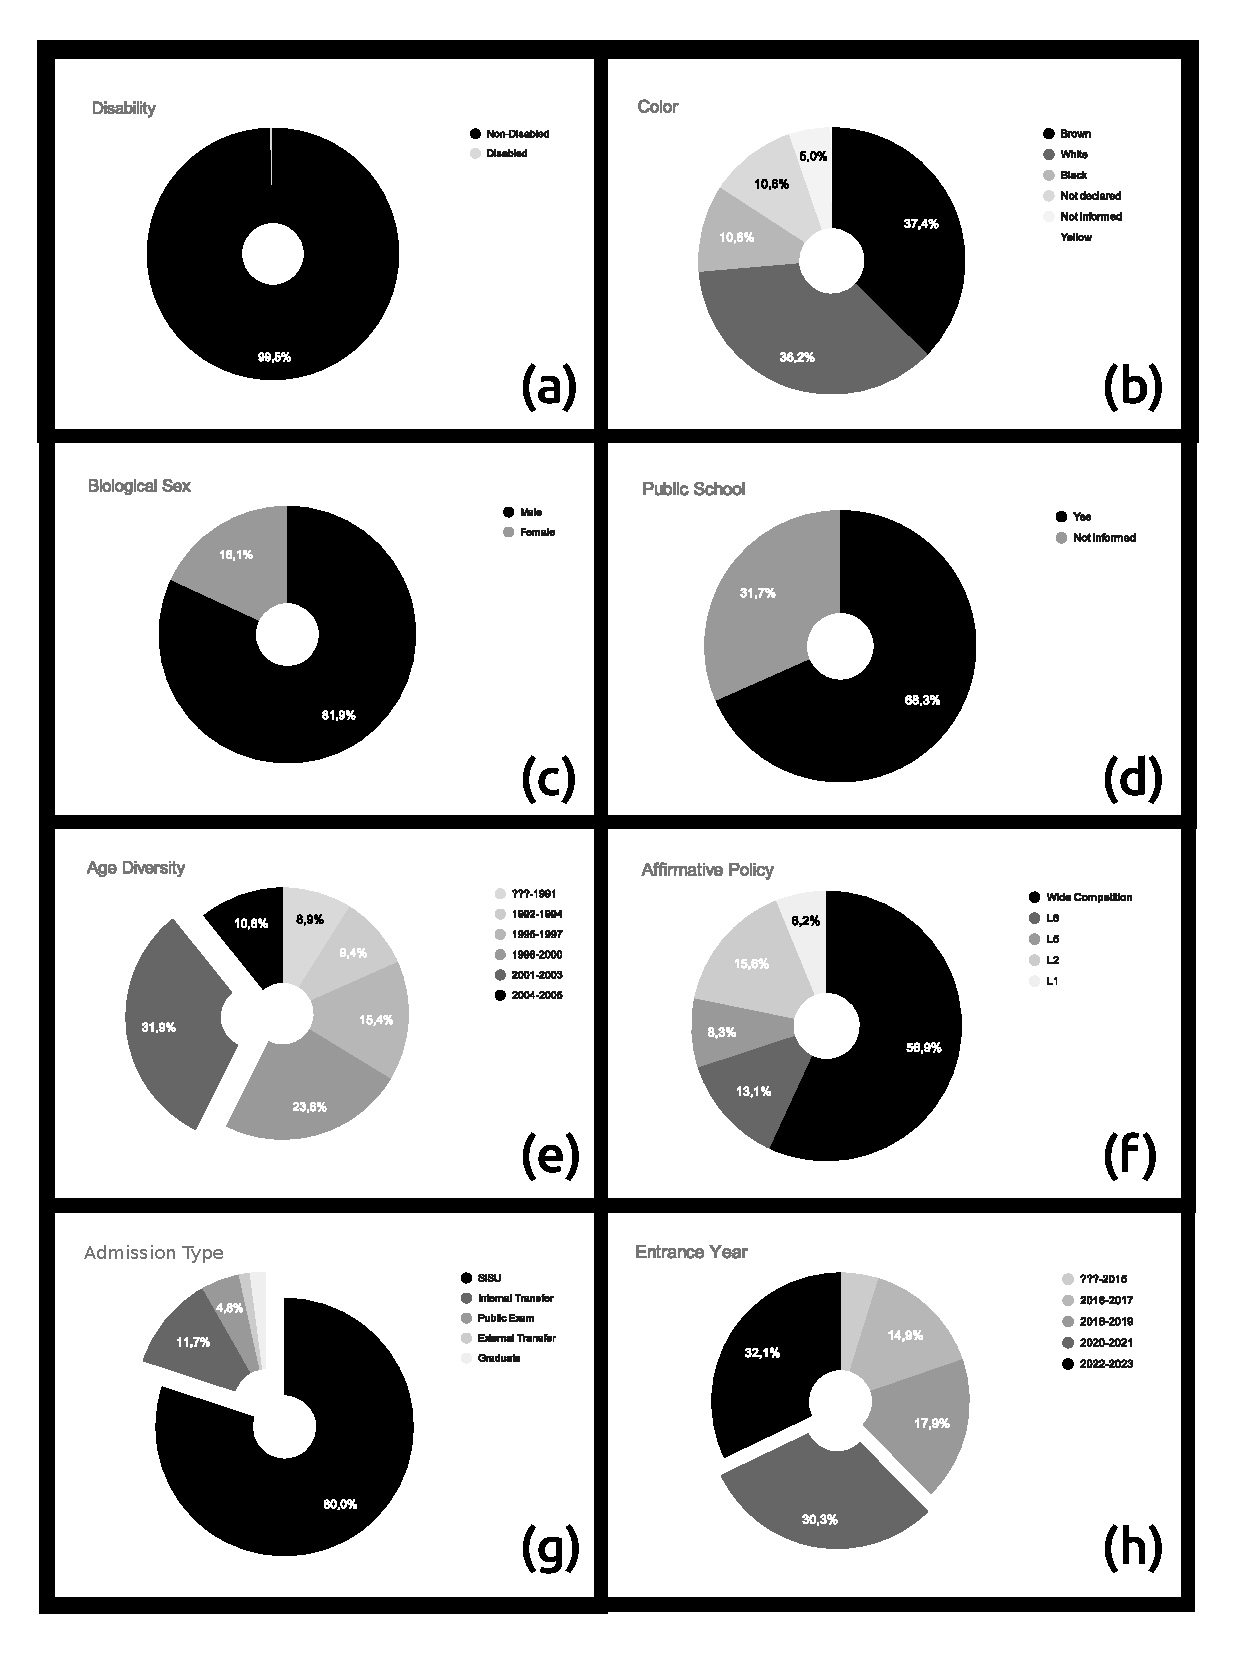
\includegraphics[width=0.9\textwidth]{images/chapter-08/all-charts-si-2023.pdf}}

\par\medskip\ABNTEXfontereduzida\selectfont\textbf{Source:} Created by the author (2024).
\end{figure}

% \fbox{
%     \begin{minipage}[htb]{0.9\textwidth}
%         \vspace{0.3cm}
                
%         \colorbox{gray!30}{% create a colored box
%             \makebox[0.975\textwidth][l]{% center the text on the page
%                 \ \ \textbf{Further Writing}
%             }
%         }

%         \vspace{0.1cm}
        
%         \begin{itemize}
%             \item Put here the aggregated report from UFPE Open Data:
%             \begin{itemize}
%                 \item situacao-academica-discentes-graduacao-2023-ufpe-atual.csv
%                 \item discentes-ingressos-sisu-2021-ufpe.csv
%                 \item discentes-ingressos-cursos-graduacao-2021-ufpe.csv
%                 \item beneficio-assistencia-estudantil-2023-proaes-ufpe.csv
%             \end{itemize}
%         \end{itemize}

%         \vspace{0.25cm}
        
%     \end{minipage}
% }

\subsection{Class Perspective}
\label{results-ss:classroom-data}

I divided the class perspective into three kinds of data sources: \gls{IS} program class planning, \acrfull{PBL} recordings, and socioeconomic form (see Table \ref{tbl:class-data-sources}).

\begin{table}[htb]
\caption{List of data sources from the class perspective (\acrshort{IS} program class planning, \acrshort{PBL} recordings, and socioeconomic form).}
\label{tbl:class-data-sources}
\centering
\rowcolors{1}{}{lightgray}
\begin{tabular}{
    >{\centering\arraybackslash}m{3cm}|
    >{\centering\arraybackslash}m{7cm}
}
    \hline
    \textbf{Abbreviation} &
    \textbf{Description} \\
    
    \hline
    \acrshort{DS-TP} &
    \acrshort{MIS} teaching plan \\
    
    \hline
    \acrshort{DS-PBL}1 &
    \acrshort{PBL}-Test data \\
    
    \acrshort{DS-PBL}2 &
    \acrshort{PBL-SEE} Output data \\

    \acrshort{DS-PBL}3 &
    \acrshort{PBL-SEE} Client Satisfaction data \\

    \acrshort{DS-PBL}4 &
    \acrshort{PBL-SEE} Performance data\\

    \acrshort{DS-PBL}5 &
    \acrshort{PBL-SEE} Content data\\

    \acrshort{DS-PBL}6 &
    \acrshort{PBL-SEE} Process data\\

    \hline
    \acrshort{DS-SEF} &
    Socioeconomic form data\\
    
    \hline
    
\end{tabular}

par\medskip\ABNTEXfontereduzida\selectfont\textbf{Source:} Created by the author (2024). \par\medskip

\end{table}

In \gls{IS} program class planning (\acrfull{DS-TP}), I collected \textbf{[DS-TP]} \gls{MIS} teaching plan 2023.1 (available in a sheet-structured format).

In \gls{PBL} recordings kind (\acrfull{DS-PBL}), I collected \textbf{[DS-PBL1]} \gls{PBL}-Test data and the assessment grades concerning each \gls{PBL-SEE} element: \textbf{[DS-PBL2]} output, \textbf{[DS-PBL3]} client satisfaction, \textbf{[DS-PBL4]} performance, \textbf{[DS-PBL5]} content, and \textbf{[DS-PBL6]} process. It is important to note that for each \gls{PBL-SEE} element, at least three data collection moments occurred through all \gls{PBL} cycles. I aggregated in Appendix \ref{chap:pbl-see-charts} all charts related to these \gls{PBL-SEE} elements. Generally, it is possible to assert that Chavo's and Quico's results in all assessment perspectives are similar, with Chavo's values slightly higher than Quico's in some situations but not disparate.

In the socioeconomic form kind (\acrfull{DS-SEF}), I collected \textbf{[DS-SEF]} a sort of data from the form available in Appendix \ref{chap:socio-quest}. I traced the Lorenz curve (Figure \ref{fig:lorenz-curve-classroom}) from each student's average household \textit{per capita} income in Chavo's and Quico’s class. I charted this curve with the data of 15 students who voluntarily answered the socioacademic questionnaire. Originally, this curve “plots the percentage of total income earned by various portions of the population when the population is ordered by the size of their incomes” \cite{gastwirth:1971}. But it helps compute several indexes to measure social inequalities, including under educational perspectives \cite{thomas:2003}. It assists us in visualizing the accumulated distribution of a certain quantity in a population.

\begin{figure}[ht!]
\centering

\caption{\textmd{Lorenz curve from average household \textit{per capita} income of Chavo and Quico’s class.}}
\label{fig:lorenz-curve-classroom}
\fcolorbox{gray}{white}{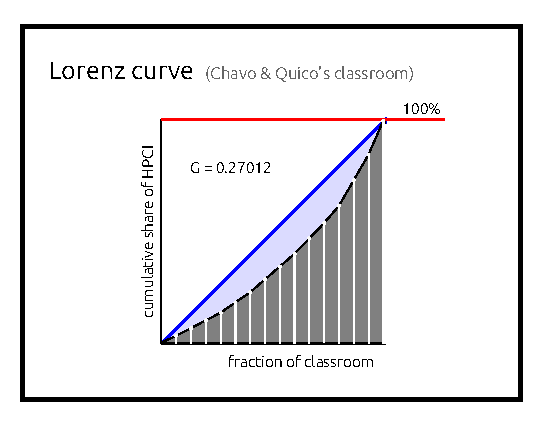
\includegraphics[width=0.9\textwidth]{images/chapter-08/lorenz-with-gini.pdf}}

\par\medskip\ABNTEXfontereduzida\selectfont\textbf{Source:} Created by the author (2024), assisted by Good Calculators (\url{http://goodcalculators.com}).%\citeauthor{manualufpe2020} (\citeyear{manualufpe2020}) \par\medskip
\end{figure}
%Data used for this chart creation :
%0.67,0.75,0.75,0.75,1.00,1.00,1.25,1.25,1.25,1.50,1.50,1.67,2.50,2.50,3.30

From Figure \ref{fig:lorenz-curve-classroom}, Chavo's and Quico's class (\acrfull{GI} $\approx$ 0.270) is closer more Finland (\gls{GI} = 0.277) than Brazil (\gls{GI} = 0.489)\footnote{Available in \url{https://data.worldbank.org/indicator/SI.POV.GINI?locations=BR}.} concerning incoming inequality. Indeed, as mentioned in Section \ref{res-meth-ss:lorenz}, \gls{GI} is a first indicator, and social inequality is a complex and multifactorial problem, but it can signal that even the Brazilian system of quotas (see Section \ref{equity-sec:br-context}) does not reflect significantly (in an \acrfull{CSE} class, for instance) the social inequality present in the Brazilian society.

Aiming to help me to choose strategically which two students I should investigate deeper (see Section \ref{res-met-ss:sampling-strategy}), I plotted the chart between student \acrfull{HPCI}s and the number of students in the \gls{MIS} class 2023.1 (Figure \ref{fig:sampling-classes-ds-sef}). I chose one \gls{CSE} undergraduate from \gls{Q}1 (Chavo) and another from \gls{Q}4 (Quico). Of all the students who disposed themselves to participate in the interview moment, three belonged to \gls{Q}1, and two belonged to \gls{Q}4. I chose Chavo (\gls{HPCI} $\approx$ 0.67 Brazilian minimum wage) and Quico (\gls{HPCI} $\approx$ 2.50 Brazilian minimum wages), picking up one \gls{CSE} student in \gls{Q}1 and \gls{Q}4 respectively and at random.

\begin{figure}[ht!]
\centering

\caption{\textmd{Chart from average household \textit{per capita} income of Chavo and Quico’s class aiming to identify the four sampling classes (from \acrshort{Q}1 to \acrshort{Q}4).}}
\label{fig:sampling-classes-ds-sef}
\fcolorbox{gray}{white}{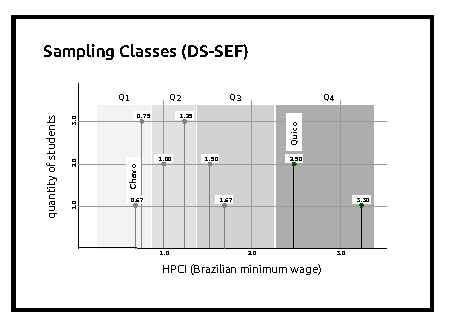
\includegraphics[width=0.9\textwidth]{images/chapter-08/collected-sampling-classes.pdf}}

\par\medskip\ABNTEXfontereduzida\selectfont\textbf{Source:} Created by the author (2024).%\citeauthor{manualufpe2020} (\citeyear{manualufpe2020}) \par\medskip
\end{figure}

% \vspace{0.3cm}

% \fbox{
%     \begin{minipage}[htb]{0.9\textwidth}
%         \vspace{0.3cm}
                
%         \colorbox{gray!30}{% create a colored box
%             \makebox[0.975\textwidth][l]{% center the text on the page
%                 \ \ \textbf{Further Writing}
%             }
%         }

%         \vspace{0.1cm}
        
%         \begin{itemize}
%             \item Creating a table with all data concerning the grades of MIS students.
%         \end{itemize}

%         \vspace{0.25cm}
        
%     \end{minipage}
% }

% \vspace{0.3cm}





  
\chapter{Discussion}
\label{chap:discussion}

 I structure this chapter into three sections, matching each \acrfull{RG} mentioned previously (see Section \ref{intro-sec:goals-pres}). Section \ref{disc-sec:sdl-trajectories} looks to understand Chavo's and Quico's \acrfull{SDL} trajectories (\gls{RG}1). Section \ref{disc-sec:sdl-capabilities} defines \gls{SDL} capabilities, mapping its main elements in Chavo's and Quico's \gls{SDL} trajectories through an analysis of the ``taking the initiative'' capability (\gls{RG}2). Finally, Section \ref{disc-sec:recommendations} presents a set of equity publications addressing guidelines to (\acrfull{CSE}) educational stakeholders concerning how to apply this discussion in their concrete context (\gls{RG}3).
\section{SDL Trajectories}
\label{disc-sec:sdl-trajectories}

Aiming to achieve \gls{RG}1, I develop the discussion about Chavo's and Quico's \gls{SDL} trajectories from two perspectives: \gls{SDL} goals (Section \ref{disc-ss:sdl-goals}) and \gls{SSDL} stages (Section \ref{disc-ss:staged-sdl}).

\subsection{SDL Goals}
\label{disc-ss:sdl-goals}

Although I presented many possibilities previously concerning \gls{SDL} contexts (e.g., personal, academic, professional), Chavo's and Quico's main focus was from the \underline{skill improvement} perspective (see Section \ref{sdl-sec:goals}). There is a central concern related to their professional improvements, potentially aiming for a better position in the labor market.

It is essential to highlight that the underlying Chavo's and Quico's conception can be that which computing refers not primarily to a personal or social transformation. \glsfirst{CEd} is an opportunity to allow them to dispute in a competitive way among the ``players'' in the labor market \cite[p.~428]{bispojr:2024-nmp}. It seems that critical reflection appears as a byproduct of this primary pursuit of a good professional positioning.

It is possible that \underline{critical reflection} is not verbalized due to business culture's tendency to be more ``professional'' during interview moments. I realize that Chavo assumed this standing during most of the interview, signaling a concern to focus on ``professional aspects'' of the answers and, consequently, avoiding a more personal tone that could express some elements in this dimension.

In Quico's case, even when the interview followed a more informal tone, his reported \gls{SDL} case about the development of a Discord bot did not flow to a critical reflection or self-human development \textit{per si}. Quico allowed himself to develop a Discord bot because this effort could promote his skill development.

In both students, the \underline{social emancipation} dimension was not captured, leading me to believe in a perspective more individualistic concerning this \gls{SDL} goals. There are no elements to assert that their group participation or the development of their self-direction sought a struggle or fight against some kind of oppressive situation. Two possibilities to understand this phenomenon better are: (i) assuming that we are living in a post-modern condition and, for this reason, there is an absence of an accepted, cohesive, and coherent society structure, leading to individuals not adhering to solid metanarratives or a "cause" that lead them to want to change or reform the society\footnote{\citeonline[pp.~278-280]{bispojr:2022-educomp} discussed deeper how the perception of identities can affect computing education.}, and (ii) realizing the search for meaning (and values) in life can contribute to the existential vacuum including in educational contexts \cite{csanli:2021}, leading students to give up to have a "solid reason" to live truly.

\subsection{SSDL Stages}
\label{disc-ss:staged-sdl}

The overall impression is Chavo is situated in the \underline{Involved and Self-Directed stages} (Stages 3 and 4) from \gls{SSDL} Grow's axis (see Table \ref{tbl:ssdl-model}). There is no strangeness for him concerning requirements to the main steps of \gls{SDL} process. It seems that Chavo handles team activities well and manages these self-study moments reasonably. I felt that Chavo is more independent and appears to assume a considerable level of commitment in his household activities. This behavior seems to facilitate him in a more proactive standing before the demands in a general way. 

In this direction, I want to point out some considerations what I am calling Context-free \gls{SDL}. We need to think about a set of  critical questions about this: (i) Are there cognitive,  metacognitive and motivational capabilities able to transpose to learn new skills across the lifespan? \cite{sheffler:2022}; (ii) Is it possible to think about "meta" \gls{SDL} competencies (or even capabilities) that can serve as a basis to other more contextualized \gls{SDL} journeys (similar to the perspective of upper-level ontologies \cite{niles:2001})?; What is it possible to transpose as a "meta-learning" from a \gls{SDL} journey to another one? These questions touch in a central problem concerning the last assertion about a more independent stance of Chavo can be contextualized in new environments like a \gls{MIS} class using a \gls{PBL} approach.

Compared to Chavo, I think Quico is situated in the \underline{Dependent and Interested stages} (Stages 1 and 2) from \gls{SSDL} Grow's axis. Quico refers during the interview to many situations in which he needed to validate his "right way" of guiding his \gls{SDL} activities. Quico always validated his choices from third persons (e.g., father, superior) in these cases. I realize this trait is a signal in two directions: (i) firstly, there is more dependency on others, leading to a little developed autonomy (or maybe even a heteronomy); or (ii) secondly, he developed an interpersonal intelligence\footnote{Howard Gardner \cite[p.~4]{gardner:1989} structured a theory of multiple intelligences, namely: (i) logical-mathematical, (ii) linguistic, (iii) musical, (iv) spatial, (v) bodily-kinesthetic, (vi) interpersonal, and (vii) intrapersonal.} that leads him to explore more human than non-human resources.

I want to outline some considerations concerning interpersonal intelligence. Depending on how someone usually develops their interpersonal competencies, there are more "suspicions" (or not) related to their self-directedness. If most of someone's interpersonal relationships are inside their family circle, thus this person tends to be considered more dependent and, consequently, less self-directed, being a dependent learner from \gls{SSDL} perspective (see Figure \ref{fig:ssdl-matrix}). This remembers the three theories of life presented by \citeonline[pp.~38,39]{tolstoy:1894}, ranging from individual, passing by tribe (or clan, family, nation), and, finally, coming to a more general principle of life (that encompasses all created things). From a humanistic viewpoint, when a person transcends an individualistic perspective towards broader levels of belonging, they embody self-directedness in its true essence.
\section{SDL Capabilities}
\label{disc-sec:sdl-capabilities}

Perceiving \gls{SDL} under the lens of competencies is not an innovative approach \cite{patterson:2002,morris:2019,colomer:2021}. In this direction, we can map each stage from Knowles' \gls{SDL} model (see Section \ref{sdl-models-ss:linear}) as a competency to be developed. However, it is necessary to ensure some minimal elements. Bearing in mind that competency can be defined as the intersection of knowledge, skills, and dispositions (e.g., \citeonline{kumar:2023} in \acrfull{CS2023}), it expects to deepen each of these dimensions for each competency.

Thus, it is not different concerning capabilities. When we decide to transpose each stage from Knowles' \gls{SDL} model as a capability, it is also necessary to develop its minimal three dimensions: (i) achieved functionings (or simply achievements), (ii) means (including goods and services), and (iii) conversion factors (see Figure \ref{fig:grouped-robeyns-representation}).
We already know that the competencies and capabilities approaches have similarities, but there are many distinctions between these two concepts \cite{lozano:2012}, being necessary that we expand and rebase our way to see competency. Thus, I call them \gls{SDL} capabilities set, being composed by (i) taking the initiative, with or without the help of others, in (ii) diagnosing their learning needs, (iii) formulating learning goals, (iv) identifying human and material resources for learning, (v) choosing and implementing appropriate learning strategies, and (vi) evaluating learning outcomes. These six capabilities are interrelated and allow us to analyze Chavo and Quico’s \gls{SDL} under the \acrfull{CA} lens\footnote{It is crucial to highlight that a \gls{CA} analysis tends to be strongly interrelated among the dimensions inside the capability set. Thus, the achievements, means, and conversion factors are expected to appear several times in all capabilities transversally.}. I describe "taking the initiative" \gls{SDL} capability in more detail as follows from its achievements (Section \ref{disc-ss:achievements}), means (Section \ref{disc-ss:means}), and conversion factors (Section \ref{disc-ss:conversion-factors}).

\subsection{Achievements}
\label{disc-ss:achievements}

In an educational equity analysis, it is crucial to identify what functionings, beings and doings (see Section \ref{sen-ss:functioning}), are already achieved by students. As the Universal Monarch of \citeonline[p.~74]{saint-exupery:1943}\footnote{The Universal Monarch is a king from one of the planets visited by the Little Prince, a classic novel written by the French pilot Antoine de Saint-Exupéry.} said, "One must require from each one the duty which each one can perform". All computing educators should consider the current functioning state of their students, seeking to understand what the following steps would be proposed for each one, not only as a learning challenge but also as a fair learning challenge. These achieved functionings are called \glspl{A}, and I identified a list of them (Table \ref{tbl:achievement-list}) concerning "taking the initiative" \gls{SDL} capability from Chavo's and Quico's interviews mainly. 

\begin{table}[ht]
\caption{Achievement list for "taking the initiative" \acrshort{SDL} capability from Chavo's and Quico's data.}
\label{tbl:achievement-list}
\centering
\rowcolors{1}{}{lightgray}
\begin{tabular}{p{0.5cm}p{8.5cm}}
\hline
\textbf{\#} &
\textbf{Achievement}\\
\hline     
A1 &
Realizing the "turning point insight".\\
A2 & 
Possessing specific previous knowledge.\\
A3 &
Having a minimum volition for. \\
A4 &
Being a non-dependent learner. \\
A5 &
Dominating a foreign language. \\
\hline

\end{tabular}
\par\medskip\ABNTEXfontereduzida\selectfont\textbf{Source:} Created by the author (2024). \par\medskip
\end{table}

This is not an exhaustive list (and I am not sure if there is any chance to do it). The aim is to enlighten and expand our vision concerning the reach that an equity analysis can embrace. I discuss two of these achievements, \gls{A}1 and \gls{A}2, in more detail as follows.

\subsubsection{Turning Point (A1)}

\gls{A}1 is "realizing the 'turning point'". Let us see what Chavo answered to a \acrfull{IQ}.6 unfolding question:
\begin{quote}
    \colorbox{black!15}{Me: Ok. [...] So, you are taking a course at the university. So, the professor requi-}
    \colorbox{black!15}{res something of you. So, is there something different that you do because this is} \colorbox{black!15}{a university subject, or does the strategy follow more or less in this same direc-} \mbox{   } \colorbox{black!15}{tion?}
    
    "It depends. It also depends on the scope that he asks us. Because, for example, in the Accounting course, the professor asked us something that he'd never asked people, which was related to building an application using management things. So... for me, it was something that he didn't give us any material for and that, in this course, I had to research it by myself. So, I had to use a different method. \underline{So... from the scope he gave me, I was researching the points}\footnote{See the original excerpt in Brazilian Portuguese in Appendix Section \ref{interview-exc-ss:chavo-iq6}.}" (underlined by me).
\end{quote}

There is a critical momentum, what I am calling turning point insight, that the learner realizes that they need to turn off the receptive (or passive) mode and turn on the active one. This capability to "change the switch" at an appropriate time is directly related to taking the initiative in a \gls{SDL} journey. This feeling helps the learner to regulate their internal dispositions concerning the problem-solving process, putting themselves in a more active role.

Why a computing educator should pay attention to the turning point insight? Because not all computing students have this achievement when they enter a classroom. These students can be required to get the turning point insight when they pursue their \gls{SDL} journey. For instance, probably, Quico does not have this achievement in a well-developed way (see Section \ref{disc-ss:staged-sdl}). Thus, if this assertion is true, the professors who adopt active approaches must map the development level of the turning point insight achievement in their classroom without leaving anyone behind.

Do I, a \gls{CSE} professor, need the turning point insight as a pre-requirement to develop \gls{SDL} activities in my class? If I do, I need to diagnose my class concerning this achievement and propose a learning pathway for all students, considering that the "box distribution" (see Figure \ref{fig:equality-vs-equity}) usually is not well-configured for my \gls{CSE} students.

\subsubsection{Specific Previous Knowledge (A2)}

\gls{A}2 is "possessing specific previous knowledge". Let us see what Quico answered to an \acrshort{IQ}.1 unfolding question:
\begin{quote}
    \colorbox{black!15}{Me: And with this programming side? Did you know anything or not? Or were you} \colorbox{black!15}{a bit of a newbie? How was that?}

    "I had a foundation, so... not too much, but I'd already seen something, do you know? I'd already seen it at other places, so... on YouTube, I'd already seen something related to programming. I focused on one there, which was Python. Afterward, I did a technical program at IF [Federal Institute] of Paulista. It lasted one and a half years. I did Maintenance and Support on Informatics. So it also had... it had programming. So, I got a larger foundation. There was this period that I got to learn by other means, there was this IF period, and now this IS [Information Systems] period, isn't it? So I'd already had there a context, even basic, but I'd already had\footnote{See the original excerpt in Brazilian Portuguese in Appendix Section \ref{interview-exc-ss:quico-iq1}.}".
\end{quote}

Chavo has also computing previous knowledge. Let us what he answered about his expectations concerning the program (\gls{IQ}.2):
\begin{quote}
    "I think I have many expectations with Management [course]. I knew I had, but I didn't know how it was... I'd never seen it a lot. I'd already studied the programming side a little bit before. I'd already lived a bit before. So, I already knew a little about what would happen. But so... this caught my attention a lot because I expected that so... I don't understand what Administration [course] is. I know that I would need to manage something in a project, project lifecycle in some course, but I didn't know how it would be. So I would have to study, so... the beginnings of Administration, Scientific Administration, and this stuff, do you know? So this changed a lot".

    \colorbox{black!15}{Me: Yes. So, didn't you have a clear perception, and this came during the program?}
    
    "Yes"\footnote{See the original excerpt in Brazilian Portuguese in Appendix Section \ref{interview-exc-ss:chavo-iq2}.}.
\end{quote}
In another Chavo's unfolding answer about how he imagine himself after graduating (\gls{IQ}.3), he mentioned his computing previous knowledge:
\begin{quote}
    "I think the technical side was always something that was easier for me because I'd already studied a bit of robotics in high school. It was something that helped me a lot, so the technical side was very good. So the management side is coming more now. Now, I'm getting to improve this\footnote{See the original excerpt in Brazilian Portuguese in Appendix Section \ref{interview-exc-ss:chavo-iq3}.}".
\end{quote}

The specific previous knowledge can help students to taking a differentiated initiative about a problem from a given domain. Thus, the depth of some initiatives depends strongly on "starting knowledge" that a person has. This matter mainly when we refer to the assessment process that may incur at risk to appraise the lack of initiative from the students' achieved results regardless where they depart from.

It is essential to highlight that both Chavo and Quico had their computing previous formation during the basic education. The inclusion of Computing in basic education around the world may contribute to a better performance in \gls{CS} programs and, consequently, reducing the retention and dropout rates. This global phenomenon has a special chapter in Brazil scenario in the latest years after the consolidation of legislation about the norms to include computing in Brazilian basic education\footnote{Available in \url{https://www.computacional.com.br/docs_oficiais/parecer_homologado.pdf}.}, promoting a better social environment to forge computing capabilities and, as a consequence, a more equitable \gls{CSE}. \citeonline{ribeiro:2023} presents this national standard for school curricula.  

\subsection{Means}
\label{disc-ss:means}

\gls{M} are available resources that a student can have or use to promote their learning. They include not only physical resources (e.g., notebooks, other goods) but also services (e.g., public transport, print quota), and even living beings. The \gls{CSE} students' freedom to pursue an expected functioning does not depend only on their achievements, needing to assess what is the availability of means. If two students have the same set of achievements but do not have the same availability of means, it is possible that the same capability is enjoyed by them at different levels. I identified a list of them (Table \ref{tbl:means-list}) concerning "taking the initiative" \gls{SDL} capability from Chavo's and Quico's interviews mainly. I discuss two of these means, \gls{M}1 and \gls{M}2, in more detail as follows.

\begin{table}[ht]
\caption{Means list for "taking the initiative" \acrshort{SDL} capability from Chavo's and Quico's data.}
\label{tbl:means-list}
\centering
\rowcolors{1}{}{lightgray}
\begin{tabular}{p{0.5cm}p{5cm}}
\hline
\textbf{\#} &
\textbf{Means}\\
\hline     
M1 &
Family's \& friends' network.\\
M2 &
Mobility. \\
M3 & 
Digital infrastructure. \\
\hline

\end{tabular}
\par\medskip\ABNTEXfontereduzida\selectfont\textbf{Source:} Created by the author (2024). \par\medskip
\end{table}

\subsubsection{Family’s \& friends’ network (M1)}

\gls{M}1 concerns the friends' network. Chavo began to answer \gls{IQ}.6 in this way: "I try to get in touch with my friends. So... those who I live more together generally"\footnote{See the original excerpt in Brazilian Portuguese in Appendix Section \ref{interview-exc-ss:chavo-iq6}.} (see Section \ref{results-ss:people}). Not having the necessary means can lead you to not pass through the "turning point" (see \gls{A}1, Section \ref{disc-ss:achievements}). As a dam gets in the inevitability of overflowing when the waters exceed its limits, there are critical success factors for \gls{SDL}. Cultivating a friends network allows you to put "more water in this dam", increasing the necessary conditions for passing through the turning point.

\gls{M}1 refers to the family's network, too. During the answer about the choice of his undergraduate program (\gls{IQ}.1), Quico shared:
\begin{quote}
    "\underline{So... we spend time there, my dad and me}, talking and so on. We saw the \acrshort{SiSU} [\acrlong{SiSU}] record, the grades... how was the situation, if it was possible to classify or not. So, by the analysis that we did, Information Systems was a program that was inside what I wanted, that was related to programming, and was also possible for me to classify"\footnote{See the original excerpt in Brazilian Portuguese in Appendix Section \ref{interview-exc-ss:quico-iq1}.} (underlined by me).
\end{quote}
Similarly, the family's network can support students in their initiative taking. Depending on which family context the student is in, they can benefit from deep and affective relationships there, contributing to their self-esteem and self-confidence. Unfortunately, in harmful family contexts, this environment can play the opposite role, not being a source of support and self-fulfillment.

\subsubsection{Mobility (M2)}

\gls{M}2 concerns the mobility of students to arrive at university. Let us what Chavo said during his answer about his weekly routine (\gls{IQ}.5):
\begin{quote}
    "So when it [my traineeship] ends at 4 pm, I leave, I get dressed literally. It's a bit rushed, but ok. I get dressed. So I have two options. \underline{Or I'm gonna walk} because it's near, so it's possible to walk without problems. I spend 20 to 25 minutes nearly". 

    \colorbox{black!15}{Me: So close.}
    
    "Not very much. \underline{Or I get on the bus}. But the bus goes at 4:20 pm. So I have to hurry up and keep my fingers crossed that it goes at 4:25 or 4:20 pm, but it's possible to get on without problems.
    
    So generally, that’s it. I have classes at college. When I come back, I get on the bus to CCEN [Exact and Natural Sciences Center], and I go to my home. So... I review the things, and I go to bed. Eating and sleeping\footnote{See the original excerpt in Brazilian Portuguese in Appendix Section \ref{interview-exc-ss:chavo-iq5}.}" (underlined by me).
\end{quote}
Concerning this same topic, Quico answered an unfolding question in this way:
\begin{quote}
    \colorbox{black!15}{Me: How do you arrive at home? Do you go by bus?}

    "\underline{I go by car}. I live in Tangamandapio. When the highway is not jammed, it's nearly 22 minutes\footnote{See the original excerpt in Brazilian Portuguese in Appendix Section \ref{interview-exc-ss:quico-iq5}.}" (underlined by me).
\end{quote}

\subsection{Conversion Factors}
\label{disc-ss:conversion-factors}

\glspl{CF} are conditions that guarantee (or not) a student to convert \glsfirst{M} to an expected functioning (e.g., \gls{CSE} competency). We can analyze them from several levels of perspectives, including personal, environmental, and social ones (see Section \ref{sen-ss:conv-fac}). I identified a list of them (Table \ref{tbl:conv-fac-list}) concerning "taking the initiative" \gls{SDL} capability from Chavo's and Quico's interviews mainly. I discuss one of these conversion factors, \gls{CF}1, in more detail as follows.

\begin{table}[ht]
\caption{Conversion factors' list for "taking the initiative" \acrshort{SDL} capability from Chavo's and Quico's data.}
\label{tbl:conv-fac-list}
\centering
\rowcolors{1}{}{lightgray}
\begin{tabular}{p{0.8cm}p{5.5cm}}
\hline
\textbf{\#} &
\textbf{Conversion Factors}\\
\hline     
CF1 &
Role Model.\\
CF2 & 
First-generation students. \\
CF3 &
Public Safety \\
CF4 &
Pandemic (sanitary crisis).\\
\hline

\end{tabular}
\par\medskip\ABNTEXfontereduzida\selectfont\textbf{Source:} Created by the author (2024). \par\medskip
\end{table}

\acrshort{CF}1 concerns role model. \citeonline[p.~2]{grande:2018} assert that role model is
\begin{citacao}
    "[...] an individual who embodies one or more desirable ways of engaging with the discipline and/or profession. Both the role model and the emulator can be a professional or a student, in any combination".
\end{citacao}
Role model plays a crucial function in computing engagement, signaling a concrete "way of being" to other members of a given community of practice. During the answer about how he imagines himself after graduating (\acrshort{IQ}.3), Chavo shared:
\begin{quote}
    "Today, many things have changed. I intend to deepen in programming: yes... but also in the cloud area, that is something I'm studying more now, and I am interested a lot. I am always interested in the [cyber]security area. So [these] are some areas that I like a lot... and programming. And my expectation is to run after to develop myself: become a junior, middle, and senior [developer], and try to be an expert in the market, a reference. \underline{I think we always want to be a reference in that we like}\footnote{See the original excerpt in Brazilian Portuguese in Appendix Section \ref{interview-exc-ss:chavo-iq3}.}" (underlined by me).
\end{quote}
In his mind, Chavo has a set of role models that help him to build and see himself in the future as a computing practitioner. These role models can serve as a source of motivation for \gls{CSE} students to take the initiative in their learning. In this case, Chavo shared with us a classic career plan route of a developer, expressing part of my understanding about his focus on skill improvement concerning \gls{SDL} goals (see Section \ref{disc-ss:sdl-goals}).

On the other hand, Quico answered \gls{IQ}.3 in this way:
\begin{quote}
    "Hmm... I intend, so... \underline{from the image that I have}, to be working in an area that I like, do you know? So... it's the first thing that comes to my mind... working on something that I like. So, deeper, maybe..., maybe... over time, if I.. in the term, I don't know... I don't know, over the  program... I can begin a traineeship and see the areas inside companies related to programming, to management... that I identify myself more. So I can follow some of them and follow my future. But guessing... clearly, I don't know, so: 'I'm gonna be developing for such company, doing such thing', do you know? \underline{It's unclear...} or I'm gonna be a project manager in a company, do you know?

    But initially, that's it. I'm gonna be working in something that I like, in some company. In the end, I'm already gonna be with a basis and to be a professional, so... well, with a certain experience due to the formation. So... that’s it. It’s unclear in my mind because I don’t have any experience in this area yet, [neither] I’m not looking for a traineeship. \underline{So maybe when I look for a traineeship and begin, it will be} \underline{clearer, do you know?}\footnote{See the original excerpt in Brazilian Portuguese in Appendix Section \ref{interview-exc-ss:quico-iq3}.}" (underlined by me).
\end{quote}
His answer reveals an unclear image of his potential future in computing. I understand that Quico also pursues skill improvement like Chavo, but it seems that he does not appropriate himself concerning the computing "ways of being". Perhaps, Chavo has "more urgency" to imagine himself as a professional than Quico due to \gls{SES} difference between them and, consequently, Chavo would need to begin his career early (and not necessarily as a voluntary and natural professional journey)\footnote{\citeonline{yerdelen:2016}, for instance, introduces the discussion about the career interest of \gls{STEM} low \gls{SES} students in
relation to some equity issues like gender and teaching level.}. 

There are many things to highlight about \gls{CF}1, but I prefer to concentrate on some points here. If we understand that a role model is essential, thus it is necessary to amplify our vision for a diversity of role models. Even inside classic computing communities of practice \cite{wenger:2002}, it is possible to identify a range of options concerning potential computing role models. \citeonline[p.~52]{guzdial:2006} pointed out the importance of creating opportunities to live in these communities from undergraduate studies:
\begin{citacao}
    "[...] Students in computer science classes are rarely working peripherally with real professional software engineers in either design or development, for example. Graduate students, on the other hand, usually are working peripherally with academic researchers, making graduate school more like legitimate peripheral participation.
    
    The best that we in traditional schooling can do is to align our instruction with the students’ perceived community of practice, i.e., the students have to believe that what they are doing and learning will lead them toward central roles in the communities of practice of their choosing. Certainly, there are different communities of practice with which a single course or degree might align, e.g., a student may take a computer science degree in order to become a software engineer, or towards becoming an intellectual property lawyer, or towards some other career where the student believes that deep knowledge of computing is important".
\end{citacao}

Another relevant question concerns the relationship between role models and \gls{CSE} curricula. Are role models a key part of our curriculum? If it is, it must have intentionality to assess the evolution of this capability. This assessment should not get restricted inside a single course, for instance, but passing through the whole \gls{CSE} program. Luckily, some students will have a good set of role models at the end of their undergraduate studies. However, it remains a question: "What is the \gls{CSE} program role (as a necessary part to form this capability in our students)?". A transversal assessment instrument is imperative to follow up their learning journey, providing adequate learning regulation. 

Observing the specific case of \acrfull{UFPE} \acrfull{IS} program, \acrfull{PBL} By-Cycles Framework helps \gls{CSE} students in this direction, promoting this authentic legitimate peripheral participation through a cyclic interaction to several stakeholders as the real client and experts from three different \gls{IS} areas (\acrfull{MIS}, \acrfull{BPM}, and \acrfull{PPM} professors). Authentic formation opportunities can concretely improve the range of computing role models, bringing these computing professionals to closer \gls{CSE} students. One aspect to consider is that this framework, in the way that was implemented in \acrshort{UFPE} \acrshort{IS} program, is more oriented to the skill improvement \gls{SDL} goal, having traits of the critical reflection (e.g., self-assessment activities like \acrshort{PBL}-Test), but no signs of a social emancipation perspective (see Section \ref{sdl-sec:goals}).

Lastly, it does not matter if Quico has \acrfull{SES} higher than Chavo in a democratic education perspective. It is a blunder to suggest that the school community should neglect Quico pursuing "justice" or a "fairer educational environment". The school community (in this case, a university) should always be a partner of a \gls{CSE} student, not their enemy. The struggle for equality of learning opportunities in \gls{CEd} must address and guarantee a common curriculum for all, regardless of their social stratum. If role models are essential to form a computing practitioner, thus every \gls{CSE} student must receive equitable teaching, providing all conditions to have these capabilities in a best-effort approach. \gls{CA} lens direct our looking to guarantee the freedom to \gls{CSE} students to develop a given expected functioning if they want to achieve it.

% I structure this section from Chavo and Quico’s answers for the following question: “Tell me about a typical day of your week”. I triangulate these answers to the findings presented in the previous section, trying to capture potential equity issues. Chavo described his daily routine as follows: 
% \begin{quote}
%     "So, now I work. I wake up at 6 am, about 6h20. So I got until... so, I rest a little, study, have breakfast between 6 and 10 am. 10 am I begin to work until midday. I come back at 1 pm, so from 1 pm to 4 pm, that is the traineeship that I got with the Federal[ Federal is an abbreviation for Federal University of Pernambuco (UFPE), his university.], so it is 6 hours.
    
%     So when it finishes at 4 pm, I get off, I get dressed literally. It's a little busy, but alright. I get dressed, so I have two options: or I go walking because it's closer, so it's easy to walk alright. It takes about 20, 25 little minutes.

%     It's a good time. Or I get a bus. But the bus is at 4h20 pm, so at this moment, it's a hurry to get dressed and cross-fingers to it passes 4h25 or 4h20, but it's easy to get it, no problem. So, in general, that's all. I have a university class. When I get off, I get the bus at CCEN [Center of Exacts and Nature Sciences]. So I go to my home, I review the things and I go to bed... eat and go to bed.

%     The week is about in this way. Weekends, I look for more to see the university things and arrange a bit the things of the week, see if there are any commitments, if I need to go for the company or if I need to go to university to study more, these things, and enjoy myself. That's all\footnote{See the original excerpt in Brazilian Portuguese in Appendix Section \ref{interview-exc-ss:chavo-iq5}.}".
% \end{quote}

% And Quico described his routine in this way:
% \begin{quote}
%     "It's in this way, I think that is... is not so ruled, but it's always the same thing. As I said to you, by the morning I have, from 10 to 14h, I'm free... Not free, I'm at home, but doing university things, maybe some domestic tasks.

%     So my day boils down to that, when it's normal when it has classes. From 10 to 14h, I'm doing any university thing, so when it comes near to 15h, I am getting dressed to come.

%     So I arrive here, I think about 14h, 16h in fact, and I am talking to folks down there. It comes the class time, we go up, so it is from 17h to 20h30 only with classes. So, practically, this boils down to that. An atypical day I think that it would be a no-class day maybe. Because I go to university usually when it happens classes, do you understand?

%     When it doesn't have classes, it doesn't have reason to go, doesn't? But... if I wouldn't have classes and I would come here, it would be more... to solve any project things that need to be everybody in a group together, you know?

%     [At the end of the day,] I arrive about 21h. When I am not talking here until 21h, I arrive at this time, 21h. So... when I'm disposed, I arrive at home... I don't know, I look at class, I look at something of class. So at the end of the day boils down basically to that, to do something of university or then entertainment".
% \end{quote}

% From the findings, there are no critical differences between the most part of \gls{SDL} capabilities of Chavo and Quico. One \gls{SDL} capability shows a significant distinction between them: time as a resource (Section \ref{results-ss:time}). It is important to understand the available time to dedicate to study as a resource, even if it is not perfectly fitted in “identifying human and material resources for learning”. Available time is a transversal resource that perpasses all \gls{SDL} capabilities, and it can affect the equality of learning opportunities.

% It is interesting to highlight that both Chavo and Quico have good grades (Section \ref{results-ss:classroom-data}) at the end of the course. But something important to ask in this scenario is if Chavo did not need to give up other capabilities (e.g., having fun at weekends), aiming to guarantee these SDL capabilities. This capabilities trade-off is an essential point to observe, therefore it can prejudice the student's well-being with severe restrictions on their available time to learn.


% The home-university-home movement is another aspect to highlight. Even Chavo living near to university, he spends in this traject the same time as Quico (who lives in a nearby city). Chavo mentioned during the interview that when he needs to bring your laptop to university, he depends on a friend’s lift to guarantee his personal safety. Probably, the Quico’s private car promotes this personal safety for him. However, the resources should not be the only key to analyzing an equity scenario; some resources can signalize critical conversion factors that can avoid to enjoy an adequate environment for learning.
\section{Recommendations}
\label{disc-sec:recommendations}

\gls{RG}3 was addressed by the arrangement of three guidelines and/or recommendations to help educational stakeholders deepen this discussion in their context. I will present each one in the next three following sections.

\subsection{Neutrality}
\label{disc-ss:neutrality}

First, other colleagues and I
structured the discussion about neutrality in \gls{CEd} \cite{bispojr:2022-educomp} from the Brazilian context, bearing in mind that it is not possible to take further steps toward equity awareness without giving up the neutrality presupposition and assuming a minimal set of democratic commitments, intentionalizing their teaching practice. This essay threw light (and some provocations) on the discussion about the supposed political-pedagogic neutrality of professors and its impacts on \gls{CSE}. It presented a little of the Brazilian context concerning the theme of political-pedagogic neutrality and its problematizations. It also exposed some struggles to understand the potential implicit agenda of supposedly neutral discourses and the importance of admitting intentionality in professor practice in \gls{CSE}. This essay still proposed a possible way to build professor identity/ies from a moderate pluralism. We made use of some authors to contribute to the deep of this discussion, like \citeonline{freire:1996-ped-aut}, \citeonline{skovsmose:2006}, \citeonline{saviani:1994}, \citeonline{hall:1992}, and \citeonline{biesta:2018}.

\subsection{LLM Equity Issues}
\label{disc-ss:llm-equity-issues}

Second, my advisors and I situated emerged equity issues from the use of \acrlong{LLM}s (\acrshort{LLM}) in (computing) education \cite{bispojr:2024-nmp}, emphasizing what we called "Prompt Literacy" and the arising of \gls{LLM}
divide due to the handling of metacognitive competencies. In the second section, we presented the digital divide, listing more common barriers to \gls{ICT} use, the potential mitigation actions for the digital divide problem, and elements to signalize the subjacent structural problem as its roots. In the third section, we described \gls{LLM}, presenting practical examples, as well as showing the opportunities and challenges of its use in educational contexts. In the fourth section, we described the arising of what we call "Prompt Literacy" redeeming the evident evolution (in terms of the complexity and impact of \gls{ICT}) from Web Access Literacy, passing by Search Engine Literacy, 
and arriving in Prompt Literacy. Lastly, we defined \gls{LLM} divide as the gap between those with ready access to \gls{LLM} tools (and the knowledge that they provide access to), and those without such access or skills. We also defined what would be an \gls{LLM} capability under the \gls{CA} lens, listing the primary sources of \gls{LLM} equity issues from this perspective.

\subsection{Equity Analysis Guidelines}
\label{disc-ss:eq-guidelines}

At last, in another work of my advisors and I, we proposed not only a basic discussion about the equity aspects of the adoption of \acrfull{OLEE} \cite{bispojr:2024-online-lab}, but also we listed a set of guiding questions to north an initial equity analysis for collective decision-making in a professor collegiate. Using a storytelling approach, we presented an Engineering Professor called Jirafales\footnote{Teacher Jirafales is one of the characters of Chespirito, a Mexican sitcom written by Roberto Bolaños.} in his journey to adopt \gls{OLEE} in his engineering program. Hypothetical situations (but potentially real) illustrated several equity issues that usually emerges in our teaching practice concerning access, literacy, and social factors. For each of these dimensions, we introduced theoretical constructs about equity from \gls{CA} lens. The idea is to pave the way for an identification with equity agenda, offering the opportunity for a professor watches themselves as part of Jirafales' dilemmas, feeling his feelings and trying to sketch a practical solution for each fictitious scenario. Empathy and theory walking together: helping each other to forge a new awareness in Engineering Education community. Finally, we created a roadmap comprising of strategic steps (one for each dimension) to follow when a collective educational space needs to conduct an equity analysis. I list the four \glspl{GQ} to consider equity in \gls{OLEE} adoption:
\begin{enumerate}
    \item \underline{Access Dimension}
    \begin{itemize}
        \item[(\gls{GQ}1)] Are there alternatives to learning in case it is impossible to access the OLEE (e.g., a physical lab version)?
        \item[(\gls{GQ}2)] Does my student (or other essential user) have real conditions to access the OLEE outside of university?
    \end{itemize} 
    \item \underline{Literacy Dimension}
    \begin{itemize}
        \item[(\gls{GQ}3)] What are the desired skills and competencies that an undergraduate should have to use my OLEE fully?
    \end{itemize}
    \item \underline{Social Dimension}
    \begin{itemize}
        \item[(\gls{GQ}4)] Is any student group disadvantaged compared to others due to OLEE use?
    \end{itemize}
\end{enumerate}
This book is expected to be published in October 2024 yet\footnote{Springer has already provided the book link: \url{https://link.springer.com/book/9783031707704}.}. 

% "It's not feasible". No, I do not agree with you. Do not ignore this pain and take the next step. Do something.




  
\chapter{Conclusions}
\label{chap:final-remarks}

 This work investigated how \gls{CSE} students conduct their \gls{SDL} in developing countries from the \gls{CA} lens (\gls{MRQ}). Three research goals helped to address this question in a qualitative approach: (i) understanding how \gls{CSE} students build their \gls{SDL} trajectories in developing countries (\gls{RG}1), (ii) mapping the main elements of \gls{SDL} capabilities observed in \gls{CSE} students in developing countries (\gls{RG}2), and (iii) recommending guidelines to (\gls{CSE}) educational stakeholders concerning how to consider effectively equity issues and active learning from the \gls{CA} lens (\gls{RG}3).

To achieve \gls{RG}1, I structured the perceptions of two \gls{CSE} Brazilian undergraduates about their \gls{SDL} trajectories, being each one from the lowest and highest \gls{SES} of their classroom, respectively. I collected and analyzed interviews primarily to construct the understanding of perceptions (Section \ref{res-sec:interviews}) with the help of other data sources to better situate the findings. At last, I discussed the results from the perspectives of \gls{SDL} goals (Section \ref{disc-ss:sdl-goals}) and \gls{SSDL} stages (Section \ref{disc-ss:staged-sdl}), locating their \gls{SDL} trajectories through this looking. 

To achieve \gls{RG}2, I analyzed the results obtained in \gls{RG}1, but from the \gls{CA} perspective (Section \ref{disc-sec:desirable-capabilities}). I proposed a new concept of \gls{SDL} capabilities, (i) identifying six of them from Knowles' process (Figure \ref{fig:sdl-process}), and (ii) examining in detail each one from the achievements, means, and conversion factors dimensions.

 Finally, to achieve \gls{RG}3, I arranged four guidelines and/or recommendations to help educational stakeholders deepen this discussion in their context. First, other colleagues and I structured the discussion about neutrality in \gls{CEd} \cite{bispojr:2022-educomp} from the Brazilian context, bearing in mind that it is not possible to take further steps toward equity awareness without giving up the neutrality presupposition and assuming a minimal set of democratic commitments, intentionalizing their teaching practice. Second, my advisors and I situated emerged equity issues from the \glspl{LLM} in (computing) education \cite{bispojr:2024-nmp}, emphasizing what we called "Prompt Literacy" and the arising of \gls{LLM} divide due to the handling of metacognitive competencies. At last, in another work of my advisors and I, we proposed not only a basic discussion about the equity aspects of the adoption of online laboratories in Engineering Education \cite{bispojr:2024-online-lab}, but also we listed a set of guiding questions to north an initial equity analysis for collective decision-making in a professor collegiate. %At last, I created a roadmap comprising of steps to follow when a collective educational space needs to conduct an equity analysis.

 In the next sections, I present the contributions and implications of my \gls{Ph.D.} journey (Section \ref{conclusions-sec:contrib-impl}), its limitations (Section \ref{conclusions-sec:limitations}), future directions and challenges (Section \ref{conclusions-sec:challenges}), and, lastly, my final remarks (Section \ref{conclusions-sec:my-final-remarks}).

 \section{Contributions and Implications}
 \label{conclusions-sec:contrib-impl}

The contributions can be divided into two groups: (i) those that originated directly from \gls{MRQ} and all \glspl{RG}, and (ii) the remaining ones that originated during the \gls{Ph.D.} period. This division is necessary because the adopted thesis format is a classic monograph, and not a paper-based thesis \cite{kubota:2021}, for example. Thus, these two kinds of contributions need to be encompassed to highlight the research contributions and also fruits fostered by \gls{CIn} postgraduate program or even resulting from other \gls{CEd} challenges that emerged during the \gls{Ph.D.} period.

\textbf{First} contribution (emerged from \gls{MRQ}) in the group (i) refers to the use of \gls{CA} as an equity theoretical framework in computing research, and \gls{CEd} mainly. There are works approaching \gls{CA} and technological areas in a generic way (e.g., Engineering \cite{fernandez:2014,odonovan:2020}), but not focusing on computing. The thesis as a whole, in a monograph format, contributes to introducing this theoretical novelty. \textbf{Second} contribution in the group (i) (emerged from \gls{RG}2) refers to the proposition of a new concept called \gls{SDL} capabilities, providing a lens to assess equity in active learning scenarios \cite{bispojr:2024-isdls}. This is a contribution to the Education area in general. \textbf{Third}, and last, contribution in the group (i) (emerged from \gls{RG}3) refers to a pragmatic instantiation of equity discussions in \gls{CSE} (mainly in \cite{bispojr:2024-online-lab} but also in \cite{bispojr:2022-educomp,bispojr:2024-nmp}). The proposition of a set of guiding
questions to orientate an initial equity analysis for an Engineering collective decision-making of professors serves this purpose, provoking them not only to change their standing but also change their actions through the following of this propositional pathway.

\textbf{First} contribution in group (ii) refers to all other relevant \gls{CEd} publications during the \gls{Ph.D.} period \cite{bispojr:2024-nmp,bispojr:2024-urca,feitosa:2024,cavalcanti:2024,pereira:2024,melo:2024-horizontes,boaventura:2024-sbgames,
boaventura:2023,esmeraldo:2023,freire:2023-rsc,freire:2023-encompif, santos:2022,bispojr:2022-educomp,esmeraldo:2022,bispojr:2021,bispojr:2021-educomp,bispojr:2021-wei,bispojr:2020-tec}. Lastly, \textbf{second} contribution in group (ii) refers to other relevant computing publications in the same period \cite{cavalcanti:2024-ieee,bispojr:2023-edi,bispojr:2023-rbie,sansil:2023,lima:2022,bispojr:2022-snee}.

I can list \textbf{two implications} of this research. \textbf{First}, it can support the Brazilian discussion in computing (and \gls{CEd}) spaces concerning \gls{DEI} agenda at more diverse levels. For example, at a local level, \gls{CoDi} is a \gls{CIn} group that discusses and fosters this agenda in a computing college at Pernambuco State. At a national level, in \gls{CEd} area, \gls{IDEA} working group \cite{pereira:2024,melo:2024-horizontes} develops this agenda inside the \gls{CEduComp} from \gls{SBC}. Still, at a national level, \gls{SBC} created the \gls{CIDE} to put this agenda inside the society at its higher organization level. \textbf{Second}, it can provide a solid material to \gls{CEd} stakeholders proposing and idealizing equity-minded syllabus \cite{anderson:2023,gama:2024} and/or curricula \cite{karimi:2024} in computing programs. This discussion is crucial not only at the Brazilian higher education level \cite{moro:2022} but also at the basic one \cite{falcao:2021}, bearing in mind that it is 
in operation, currently, a new National Standard for School Curricula \cite{ribeiro:2023}.

 \section{Limitations}
 \label{conclusions-sec:limitations}

One limitation is the epistemological nature of this research. Due to the choice of qualitative research as a methodological presupposition, it is not possible to make statistical generalizations from my findings. However, we can make analytic generalizations \cite{kennedy:1979}, signaling for future contextualizations.

Another limitation is underusing all collected data in this research, impeding the exploration and enriching of the results to understand the phenomenon better. For instance, I interviewed 12 students altogether. Two of them were only chosen as purposeful samples, but I could deepen my knowledge of these two by triangulating the sample findings with other students' data.

The last limitation is the participation withdrawal during the data collection. The first signaling came from 30 students (signing the consent form). Unfortunately, only 15 answered the socioeconomic questionnaire, and 12 participated in interviews. Analyzing from the gender lens, for example, three women answered the socioeconomic questionnaire, and none participated in interviews. I get a feeling that it emerged hesitation among them (being woman or not), maybe with a fear that their course performance could be affected depending on what they would say to me during the research.

 \section{Future Directions and Challenges}
 \label{conclusions-sec:challenges}
 
\subsection{Future Directions}

One of the future directions of this research is to investigate this phenomenon from the perspective of other stakeholders. Equity is complex and requires a multidimensional evaluation to guarantee more qualified information to provide a better decision. This research focuses on the students' watchful eyes, but it can be enriched with other fertile data sources like professors, educational managers, and other stakeholders.

Another future work resides in the examination of collected data not yet explored properly during the \gls{Ph.D.} period. As mentioned previously (Section \ref{conclusions-sec:limitations}), it is possible to delve into other interview transcripts or even collected documents to deepen the knowledge about this phenomenon by triangulating the sample findings with other student data. 

In Section \ref{intro-sec:overview}, I mentioned that \gls{CA} can help to fill some gaps during equity analysis using only the
\gls{CAPE} framework. In this direction, I shimmer two exciting research directions. First, comparing \gls{CA} and \gls{CAPE} equity analysis in detail, pointing out the strengths and weaknesses of each one. Second, it is promising to merge \gls{CAPE} with \gls{CA}, aiming to usufruct the strengths of the two approaches, creating a hybrid framework.

Lastly, the scoping mapping review in this \gls{Ph.D.} research (Chapter \ref{chap:rel-work}) stopped in the second iteration. It would be crucial to \gls{CEd} community to continue the snowballing approach, conducting the remaining iterations. The \gls{SRQ} and \glspl{DSRQ} coverage contribute significantly to mapping the broader area, paving the way for future works.


% \vspace{0.3cm}

%  \fbox{
%     \begin{minipage}[htb]{0.9\textwidth}
%         \vspace{0.3cm}
                
%         \colorbox{gray!30}{% create a colored box
%             \makebox[0.975\textwidth][l]{% center the text on the page
%                 \ \ \textbf{Further Writing}
%             }
%         }

%         \vspace{0.1cm}
        
%         \begin{itemize}
%             \item Finish mapping review.
%         \end{itemize}

%         \vspace{0.25cm}
        
%     \end{minipage}
% }

\subsection{Challenges}

 One of the challenges is continuing this research toward what is called "negative capabilities" \cite{unterhalter:2020}. The idea of negative capability refers to situating some limits of what is measurable and framing aspects of the education process associated with uncertainty and public scrutiny of complexity. For example, how can we investigate when a student "gives up" from a capability aiming to guarantee another one? There are scenarios in South Global contexts where students usually sacrifice their well-nourishment, aiming to get money or time to accomplish a certain kind of academic demand. Knowing better in which settings these "trade-offs" occur in \gls{CEd} matters.

 Another promissory way to investigate in depth is equity in \gls{CEd} under the lens of existential analysis. Equity issues are usually related to existential adversities, leading all involved people to reflect (and even question) the \gls{MiL} \cite{manco:2021}. In some scenarios, students intentionally sacrifice some of their capabilities on behalf of promoting \gls{MiL} like values, a sense of purpose, or even a reason to continue to live. Beyond this, it is possible to use Durkheim's Fatalistic Suicide Typology \cite{godor:2017} better to understand \gls{CEd} dropout phenomenon, extending the \gls{MiL} idea to a more specific "meaning in academic life".

 \section{My Final Remarks}
 \label{conclusions-sec:my-final-remarks}

 These are my final remarks. I tried to be a researcher in a holistic way within my limitations but with my best effort. I searched to be active in both serving my research community and sharing part of my research results in several scientific venues. I tried to pursue my \gls{Ph.D.} research goals with great dedication. I think this journey report can be helpful for the computing community in promoting education more fairly and responsibly. I did my best, and for this reason, I am sure that I explored my available capabilities and put them in the service of the research community. I finish this formation cycle with joy and a bit of tiredness, but also with a sense of accomplishment.

  I have a dream that, one day, equity analysis will be an integrated part of \gls{CEd} formative assessment. Computing exists because people exist. People are complex and need to be considered in a systemic approach where possible. May our common goal be for a more humanized \gls{CEd}.



  
  % % exemplo de organização interna de um capítulo separando por mais de um arquivo

  \chapter{Texto Texto Texto}
\label{chap:intro}


 Texto \textit{text} texto texto texto texto texto texto texto texto texto texto texto texto texto texto texto texto texto texto texto texto texto texto texto texto texto texto texto texto texto texto texto texto texto texto texto, no \gls{MEC}.

 Segundo \citeonline{manualufpe2020}, o \gls{MEC}, texto texto texto texto texto texto texto texto texto texto texto texto texto texto texto texto texto texto texto texto texto texto texto texto texto texto texto texto texto texto texto texto texto texto texto texto .
 
 \begin{citacao}
 Texto \textit{text} texto texto texto texto texto texto texto texto texto texto texto texto texto texto texto texto texto texto texto texto texto texto texto texto texto texto texto texto texto texto texto texto texto texto texto texto texto texto texto texto texto \cite{manualufpe2020}.  
 \end{citacao}


 
 

  \section{Texto Texto Texto}
\label{motivacao}

Texto texto texto texto texto texto texto texto texto texto texto texto texto texto texto texto texto texto texto texto texto texto texto texto texto texto texto texto texto texto texto texto texto texto texto texto, \textbf{exemplo} sigla \gls{UFPE}.

\input{images/captitulo1/figuraex}

Texto texto texto texto texto texto texto texto texto texto texto texto texto texto texto texto texto texto texto texto texto texto texto texto texto texto texto texto texto texto texto texto texto texto texto texto, conforme Figuras \ref{fig:figuraex} e Figuras \ref{fig:figuraex2}, continua no Capítulo \ref{chap:outrocapitulo}.


\input{images/captitulo1/figuraex2}

Texto texto texto texto texto texto texto texto texto texto texto texto texto texto texto texto texto texto texto texto texto texto texto texto texto texto texto \gls{UFPE}.

  
%  \input{chapters/introducao/problemahipotese.tex}
 
 \section{Texto Texto Texto}
\label{objetivos}
Texto texto texto texto texto texto texto texto texto texto texto texto texto texto texto texto texto texto texto texto texto texto texto texto texto texto texto texto texto texto texto texto texto texto texto texto.

Texto texto texto texto texto texto texto texto texto texto texto texto texto texto texto texto texto texto texto texto texto texto texto texto texto texto texto texto texto texto texto texto texto texto texto texto.

\subsection{Texto Texto Texto}
\label{sub:exemplonivel3}

Texto texto texto texto texto texto texto texto texto texto texto texto texto texto texto texto texto texto texto texto texto texto texto texto texto texto texto texto texto texto texto texto texto texto texto texto.

\subsubsection{Texto texto texto texto}
\label{subsub:exemplonivel4}

Texto texto texto texto texto texto texto texto texto texto texto texto texto texto texto texto texto texto texto texto texto texto texto texto texto texto texto texto texto texto texto texto texto texto texto texto.
      
% \input{chapters/introducao/organizacao.tex}

% .... 

  % \chapter{Texto Texto Texto}
\label{chap:outrocapitulo}

Texto texto texto texto ''texto'' texto texto texto texto texto texto texto texto texto texto texto texto texto texto texto texto texto texto texto texto texto texto texto texto texto texto texto texto texto texto texto, confome Tabela \ref{tbl:tabelaex} e a Tabela \ref{tbl:tabelaex2}.

%exemplo de inputs, ideal para organização e troca de posicionamento futuro é ter um elemento por arquivo

%usar um gerador é uma opção https://www.tablesgenerator.com/
% observação, segundo a biblioteca tableas não podem ter nenhuma linha vertical

\begin{table}[ht]
\caption{Texto Texto Texto}
\label{tbl:tabelaex}
\centering
\rowcolors{1}{}{lightgray}
\begin{tabular}{p{6cm}p{9cm}}
\hline
\multicolumn{1}{c}{\textbf{Coluna A}} & \multicolumn{1}{c}{\textbf{Coluna B}}  \\
\hline     
\textbf{coluna1} & Texto Texto Texto Texto Texto Texto Texto Texto Texto Texto Texto Texto.
\\ 

coluna2 & Texto Texto Texto Texto Texto Texto Texto Texto Texto Texto Texto Texto.              
\\ 

coluna3 & Texto \textit{Texto} Texto Texto Texto Texto Texto Texto Texto Texto Texto Texto.     
\\ \hline

\end{tabular}

  \par\medskip\ABNTEXfontereduzida\selectfont\textbf{Fonte:} Elaborada pelo autor (2020) \par\medskip
\end{table}



%usar um gerador é uma opção https://www.tablesgenerator.com/
% observação, segundo a biblioteca tableas não podem ter nenhuma linha vertical

\begin{table}[ht]
\caption{Texto Texto Texto}
\label{tbl:tabelaex2}
\centering
\rowcolors{1}{}{lightgray}
\begin{tabular}{p{6cm}p{9cm}}
\hline
\multicolumn{1}{c}{\textbf{Coluna A}} & \multicolumn{1}{c}{\textbf{Coluna B}}  \\
\hline 
coluna1 & Texto Texto Texto Texto Texto Texto ''Texto'' Texto Texto Texto Texto Texto.
\\ 

coluna2 & Texto Texto Texto Texto Texto Texto Texto Texto Texto Texto Texto Texto.              
\\

coluna3 & Texto \textit{Texto} Texto Texto Texto Texto Texto Texto Texto Texto Texto Texto.     
\\ \hline

\end{tabular}

  \par\medskip\ABNTEXfontereduzida\selectfont\textbf{Fonte:} \citeauthor{manualufpe2020} (\citeyear{manualufpe2020}) \par\medskip
\end{table}


\section{Texto Texto}
\label{sec:section}

Texto texto texto texto ''texto'' texto texto texto texto texto texto texto texto texto texto texto texto texto texto texto texto texto texto texto texto texto texto texto texto texto texto texto texto texto texto texto \cite{gil2002elaborar}.


\section{Texto Texto}
\label{sec:outrasection}

Texto texto texto texto ''texto'' texto texto texto texto texto texto texto texto texto texto texto texto texto texto texto texto texto texto texto texto texto texto texto texto texto texto texto texto texto texto texto

\subsection{Texto Texto Texto}
\label{sub:outrasubsectiona}

Texto texto texto texto ''texto'' texto texto texto texto texto texto texto texto texto texto texto texto texto texto texto texto texto texto texto texto texto texto texto texto texto texto texto texto texto texto texto


\subsubsection{Texto Texto Texto Texto}
\label{subsub:outrasubsubsection}

Texto texto texto texto ''texto'' texto texto texto texto texto texto texto texto texto texto texto texto texto texto texto texto texto texto texto texto texto texto texto texto texto texto texto texto texto texto texto

\subsubsection{Texto Texto Texto Texto}
\label{subsub:outrasubsubsection2a}

Texto texto texto texto ''texto'' texto texto texto texto texto texto texto texto texto texto texto texto texto texto texto texto texto texto texto texto texto texto texto texto texto texto texto texto texto texto texto

%a organização fica a seu critério se preferir utilize inputs para cada seção, subseção etc...
%apenas um exemplo de subseção em arquivo para ser incluido
\subsection{Texto Texto Texto}
\label{sub:outrasubsection2}

Texto texto texto texto ''texto'' texto texto texto texto texto texto texto texto texto texto texto texto texto texto texto texto texto texto texto texto texto texto texto texto texto texto texto texto texto texto texto


\subsubsection{Texto Texto Texto Texto}
\label{subsub:outrasubsubsection2}

Texto texto texto texto ''texto'' texto texto texto texto texto texto texto texto texto texto texto texto texto texto texto texto texto texto texto texto texto texto texto texto texto texto texto texto texto texto texto

%apenas um exemplo de subseção em arquivo para ser incluido

\section{Texto Texto}
\label{sec:section3}

Texto texto texto texto ''texto'' texto texto texto texto texto texto texto texto texto texto texto texto texto texto texto texto texto texto texto texto texto texto texto texto texto texto texto texto texto texto texto
  
  % \chapter{Texto Texto Texto}
%não se esqueça de definir uma label única para utilizar no comando \ref
\label{chap:metodologia}

Texto texto texto texto texto texto texto texto texto texto texto texto texto texto texto texto texto texto texto texto texto texto texto texto texto texto texto texto texto texto texto texto texto texto texto texto.

%exemplos de parágrafos com footnote
Texto texto texto texto texto texto texto texto texto texto texto texto texto texto texto texto texto texto texto texto texto texto texto texto texto texto texto texto texto texto texto texto texto texto texto texto \textit{Footnote} \footnote{Segundo \citeonline{manualufpe2020}, Exemplo de nota de rodapé.}.

\section{Texto Texto}
\label{sec:algumlabel}

Texto texto texto texto texto texto texto texto texto texto texto texto texto texto texto texto texto texto texto texto texto texto texto texto texto texto texto texto texto texto texto texto texto texto texto texto.

Texto texto texto texto texto texto texto texto texto texto texto texto texto texto texto texto texto texto texto texto texto texto texto texto texto texto texto texto texto texto texto texto texto texto texto texto \textit{Footnote} \footnote{Segundo \citeonline{manualufpe2020}, Exemplo de nota de rodapé 2.}.

%exemplo de código fonte, as configurações estão no arquivo packages.tex
\lstinputlisting[language=PHP, 
caption=Texto texto texto texto
,label=lst:exemplocodigo1]{chapters/trechos_codigo/funcoescatdinamicas.m}

\hspace{4cm}
\hfill
\begin{minipage}[t]{.65\textwidth}
\ABNTEXfontereduzida\selectfont\textbf{Fonte:} Elaborado pelo autor (2020) 
\end{minipage}


Texto texto texto texto texto texto texto texto texto texto texto texto texto texto texto texto texto texto texto texto texto texto texto texto texto texto texto texto texto texto texto texto texto texto texto texto, referente ao Código Fonte \ref{lst:exemplocodigo1} função \texttt{nome\_funcao}.

\subsection{Texto Texto Texto}
\label{subsec:algumlabel}

Texto texto texto texto texto texto texto texto texto texto texto texto texto texto texto texto texto texto texto texto texto texto texto texto texto texto texto texto texto texto texto texto texto texto texto texto.

\section{Texto Texto}
\label{sec:algumlabel2}
%exemplo de quadro
Texto texto texto texto texto texto texto texto texto texto texto texto texto texto texto texto texto texto texto texto texto texto texto texto texto texto texto texto texto texto texto texto texto texto texto texto, ver Quadro \ref{quad:exemplo_de_quadro}.

%a diferença do quadro pra tabela é que o quadro tem linhas verticais
\begin{quadro}
\caption{Texto texto texto texto texto}
\label{quad:exemplo_de_quadro}
\centering
\begin{tabular}{|lllll|}
\cline{1-5}
A& B &  C& D &E  \\ \cline{1-5}
\multirow{3}{*}{1}  & 2 &  3& 4& 5 \\
 &  2 &  3& 4& 5  \\
 &  2 &  3& 4& 5 \\
 \cline{1-5}
\end{tabular}
  \par\medskip\ABNTEXfontereduzida\selectfont\textbf{Fonte:} Elaborada pelo autor (2020) \par\medskip
\end{quadro}


\subsection{Texto Texto Texto}
\label{subsec:algumlabel2}
Texto texto texto texto texto texto texto texto texto texto texto texto texto texto texto texto texto texto texto texto texto texto texto texto texto texto texto texto texto texto texto texto texto texto texto texto.

\subsection{Texto Texto Texto}
\label{subsec:algumlabel3}

Texto texto texto texto texto texto texto texto texto texto texto texto texto texto texto texto texto texto texto texto texto texto texto texto texto texto texto texto texto texto texto texto texto texto texto texto.


  % \chapter{Texto Texto Texto}
\label{chap:capitulo1}

Texto texto texto texto texto texto texto texto texto texto texto texto texto texto texto texto texto texto texto texto texto texto texto texto texto texto texto texto texto texto texto texto texto texto texto texto.


\lstinputlisting[language=Java, 
caption=Texto texto texto texto
,label=lst:exemplocodigo2]{chapters/trechos_codigo/java.m}
\hfill
\begin{minipage}[t]{.65\textwidth}
\ABNTEXfontereduzida\selectfont\textbf{Fonte:} \citeauthor{universidadejava2020}  (\citeyear{universidadejava2020}) 
\end{minipage}




\section{Texto Texto Texto}
\label{sec:label}
Texto texto texto texto texto texto texto texto texto texto texto texto texto texto texto texto texto texto texto texto texto texto texto texto texto texto texto texto texto texto texto texto texto texto texto texto, ver Capítulo \ref{chap:metodologia}, Seção \ref{sec:algumlabel}.

Texto texto texto texto texto texto texto texto texto texto texto texto texto texto texto texto texto texto texto texto texto texto texto texto texto texto texto texto texto texto texto texto texto texto texto texto (Código Fonte \ref{lst:exemplocodigo2}).


\section{Texto Texto}
\label{sec:outralabel}

Texto texto texto texto texto texto texto texto texto texto texto texto texto texto texto texto texto texto texto texto texto texto texto texto texto texto texto texto texto texto texto texto texto texto texto texto.



\bookmarksetup{startatroot}% 


% ----------------------------------------------------------
% ELEMENTOS PÓS-TEXTUAIS
% ----------------------------------------------------------
\postextual


% ----------------------------------------------------------
% Referências bibliográficas
% ----------------------------------------------------------
\bibliographystyle{abntexalfenglish} %caso seja em inglês, retire o comentário desta linha

% \renewcommand{\bibname}{REFER\^ENCIAS}
%\renewcommand{\bibname}{Bibliography}
% \addbibresource{sample.bib}
\bibliography{references2}


% ----------------------------------------------------------
% Apêndices
% ----------------------------------------------------------


% ----------------------
% força para que não exiba subtítulos em apêndices no sumário
% -----------------------

\begin{apendicesenv}
\addtocontents{toc}{\protect\setcounter{tocdepth}{1}}
\makeatletter
\addtocontents{toc}{%
  \begingroup
  \let\protect\l@chapter\protect\l@section
  \let\protect\l@section\protect\l@subsection
}
\makeatother

% Imprime uma página indicando o início dos apêndices
% \partapendices

%coloca o identificador do anexo/apendice somente na primeira página
\chapter{Publications}
\label{chap:appendix-a}

This section presents my publications in computing education (Section \ref{ap-other-writings:comp-ed}) or related areas (Section \ref{ap-other-writings:related-areas}). This section outlines general interests, and formative trajectories traveled during my doctoral studies. At the end of this section, I present the list of all publications presented here (Table \ref{tbl:publications}).

\section{Writings in Computing Education}
\label{ap-other-writings:comp-ed}

At the end of 2020, my colleagues and I published a Portuguese paper to present the distinction between Computing Education and Informatics in Education areas \cite{bispojr:2020-tec}. In Brazil, even among computing researchers, there is confusion about the epistemological roots of these two areas. To highlight these knowledge frontiers, we outlined preliminary considerations about the convergence between them, what we called Technologies in Computing Education. This paper aimed to establish a dialog between these areas, enriching potential research emerging from this meeting. It was published in the Brazilian Journal of Computers in Education \gls{RBIE}\footnote{RBIE stands for "Brazilian Journal of Computers in Education" in English.}. This paper has been a reference for authors who submit their papers on Track "Digital Technologies for the Development of Computational Thinking and Computing Education" at the \gls{SBIE}\footnote{SBIE stands for "Brazilian Symposium of Informatics on Education" in English.} since 2020.

At the beginning of 2021, I wrote, together with some researchers, a Portuguese essay, bringing reflections and challenges about the formation of research ethics in Computing involving humans \cite{bispojr:2021-wei}. This essay approached this subject both in a general context and the specific context of Computing. I presented this paper at the most traditional \gls{CEd} workshop in Brazil (\gls{WEI}).

In April 2021, I presented a case study discussing the impact of Peer Instruction use on a \gls{CSE} course \cite{bispojr:2021-educomp} at the \gls{EduComp}\footnote{EduComp stands for "Brazilian Symposium of Computing Education" in English.}. I wrote this Portuguese paper in collaboration with the pedagogue Prof. Rosemara Lopes. We were honored to be one of the best papers of \gls{EduComp} 2021. As a consequence, \gls{RBIE} invited us to extend it for an English paper \cite{bispojr:2021}. 

In \gls{EduComp} 2022, I had the opportunity to share an essay problematizing the supposed neutrality of the computing professor \cite{bispojr:2022-educomp}. I wrote this Portuguese paper in partnership with computing and education researchers.

At the beginning of 2022, an extension paper was published in a journal called Springer Notes in Computer Science \cite{santos:2022}. This English paper was conducted mainly by my advisor, Prof. Simone Santos, counting on my collaboration. This work presents a diagnosis of \gls{CSE} at the Brazilian public institutions about their readiness to implement \gls{PBL}.

In February 2022, \gls{CNE}\footnote{CNE stands for "National Council of Education (CNE)" in English.} homologated the norms to include computing in Brazilian basic education\footnote{Available in \url{https://www.computacional.com.br/docs_oficiais/parecer_homologado.pdf}.} as a complement to \gls{BNCC}\footnote{BNCC stands for "Common National Curricular Basis" in English.}. \gls{CNE} is linked to \gls{MEC}\footnote{MEC stands for "Brazilian Ministry of Education" in English.} that helps in the regulation of Brazilian legislation concerning Education at a national level. These norms were proposed by a working group which I had the honor to make part of. In this working group, my team was responsible for structuring the computing competencies appropriate for the early childhood education level\footnote{The full text of this \gls{BNCC} complement is available in \url{https://www.computacional.com.br/docs_oficiais/Tabelas-Computacao.pdf}.}.

In May 2022, I could share a Portuguese abstract about ethnocomputing \cite{bispojr:2022-snee} during the \gls{SNEE}\footnote{SNEE stands for "Northeast Symposium of Ethnobiology and Ethnoecology" in English.}. This work was written in collaboration with two computing education researchers and described ethnocomputing through its interest’s problems. It was so exciting to divide these concerns into a different research community.

In July 2022, I had the opportunity to present the research results developed in Ceará state, in the Brazilian Northeast. This paper \cite{esmeraldo:2022} was shared at the \gls{AIED} on the Practitioner track, being the fruit of a partnership between \gls{IFCE} and \gls{UFJ}. This work contributed to computing education by proposing an algorithm to help teachers to identify at-risk students previously using genetic programming and linear regression.

In the middle of 2023, a Portuguese paper was published in \gls{ENCompIF} reporting a methodological perspective of using question answering in programming learning \cite{freire:2023-encompif}. This research was conducted at \gls{IFCE} primarily with my collaboration and other colleagues from \gls{UFCG} and University of Groningen. After the invitation of \gls{ENCompIF}\footnote{ENCompIF stands for "Computing National Meeting of Federal Institutes" in English.} chairs, we published a Portuguese extended version of this paper in \gls{RSC}\footnote{RSC stands for "Systems and Computing Journal" in English.} \cite{freire:2023-rsc}, including also Bard \gls{LLM} in the analysis (beyond \gls{BERT} and ChatGPT).

Still in the middle of 2023, a \gls{RBIE} Portuguese paper was published presenting an approach to simplify learning through the practice of projects of computational systems in a simulation environment \cite{esmeraldo:2023}. This paper was another collaboration with \gls{IFCE} researchers, including Prof. Edna Barros (\gls{CIn}) and other colleagues from \gls{IFS} and \gls{UECE}.

In September 2023, I had the privilege to share in-person part of the results of our \gls{UFJ} teaching project \cite{boaventura:2023} in the \gls{ICL} that happened at Madrid, Spain. This work reported the experience of integrating aspects of innovation and entrepreneurship in \gls{IPC} in a Brazilian context, more specific at Goiás state. There was collaboration of \gls{UECE} and \gls{IFCE} researchers, beyond of my advisor Prof. Simone Santos.

In November 2023, I participated in \gls{NMP} with a short presentation about the equity issues derived from use of \gls{LLM} in education. \gls{NMP} is organized by Prof. Łukasz Tomczyk of the Institute of Education at the Jagiellonian University (Poland), funded by the Polish \gls{NAWA}. He invited my advisors and me to submit a full paper based in the extension of the ideas of my initial presentation. This paper was accepted and published as a Springer book chapter \cite{bispojr:2024-nmp}.

In February 2024, I presented (remotely) part of the first findings of \gls{RG}1 and \gls{RG}2 \cite{bispojr:2024-isdls} in the 37$^{\mbox{th}}$ \gls{ISDLS} happened at Florida, \gls{USA}. I wrote this work in partnership with my advisors during the sandwich doctorate (interchange period) at Brunel University London in the \gls{UK}.

In July 2024, \gls{IJAIED} published a paper that shows a proposal for integrating pedagogical guidelines founded on competencies and skills by leveraging an educational recommendation system in a Brazilian case perspective \cite{feitosa:2024}. I collaborated on this work that uses ontologies generated from teacher and student responses, beyond ontology alignments between them, and, at last, personalized action recommendation algorithms to minimize each student’s cognitive deficiencies.

In September 2024, a hybrid intervention applied to the \gls{IoT} course using \gls{PBL} and Maker Culture was presented in the \gls{ICL} \cite{cavalcanti:2024}. I could collaborate in this case study that assessed both the students' learning effectiveness and theory-practice integration of a Brazilian \gls{IoT} course.

\section{Writings in Related Areas}
\label{ap-other-writings:related-areas}

In December 2022, the research results related to the pedagogical use of the Gather tool during emergency remote learning at the postgraduate level were published in the \gls{LS}\footnote{L\&S stands for "Language \& Society Booklet" in English.} journal. This Portuguese paper \cite{lima:2022} was the fruit of an intervention conducted by me during the course “Education and Society” taught by Prof. Sérgio Abranches at the \gls{UFPE} Education Center. Gather tool simulates an \gls{RPG} world, promoting a more immersive experience during remote learning.

Before applying to this \gls{Ph.D.}. program, I published a theoretical paper on the philosophy of informatics in education \cite{bispojr:2019}. This Portuguese paper presented two epistemological issues about the knowledge nature produced in Educational Data Mining: (i) a question of ontological nature about the content of the obtained knowledge and (ii) a question of deontological nature about the guidelines and principles adopted by education researchers, to the detriment of the results of their research. In the end, I outlined some considerations and guidelines as a result of the discussion of the issues raised. I presented this paper at \gls{SBIE}. Four years later, when I was already a \gls{Ph.D.} student, I published an extension of this paper focusing on equity issues, specifically \cite{bispojr:2023-edi}. I presented this extension at the \gls{EDI} during \gls{AIED}.

Yet in collaboration with other education researchers, I published a Portuguese paper \cite{bispojr:2023-rbie} in \gls{RBIE} journal, presenting the contrasts and convergences between two teachers of public high schools of Pernambuco state, Brazil, concerning digital inclusion during and after emergency remote teaching. This work arose from a final project of the same course, “Education and Society”, taught by Prof. Sérgio Abranches. We had the opportunity to extend this work and also publish it as a book chapter \cite{sansil:2023}.

 Lastly, on release schedule in November 2024, Springer will publish the book "Online Laboratories in Engineering and Technology Education: State of the Art and Trends for the Future". My advisors and I had an accepted chapter in this book \cite{bispojr:2024-online-lab}, discussing the equity aspects of the adoption of \gls{OLEE}. Addressing part of \gls{RG}3, we proposed a list of guiding questions to consider equity in \gls{OLEE} adoption, making it possible to adapt it for \gls{CEd} in an effortless way.

\begin{table}[ht]
\caption{List of publications during my \acrshort{Ph.D.} journey.}
\label{tbl:publications}
\centering
\rowcolors{1}{}{lightgray}
\begin{tabular}{
    >{\centering\arraybackslash}m{5.5cm}|
    >{\centering\arraybackslash}m{5.4cm}|
    >{\centering\arraybackslash}m{3.1cm}
}
    \hline
    \multicolumn{2}{c|}{
        \textbf{Full}
    } &
    \textbf{Short/} \\
    \cline{1-2}
    \textbf{Journal} &
    \textbf{Conference} & 
    \textbf{Abstract}\\
    \hline 
    \cite{feitosa:2024}     
     &
        \cite{bispojr:2024-isdls}
        \newline
        \cite{bispojr:2024-nmp}$^*$
        \newline
        \cite{cavalcanti:2024-ieee}
        \newline
        \cite{cavalcanti:2024}     
    &
    \cite{pereira:2024}
    \newline
    \cite{boaventura:2024-sbgames}
    \newline
    \cite{bispojr:2024-urca}\\
    \hline
    
    \cite{bispojr:2023-rbie}
    \newline
    \cite{esmeraldo:2023}
    \newline
    \cite{freire:2023-rsc} &
    
    \cite{bispojr:2023-edi}
    \newline
    \cite{boaventura:2023} 
    \newline
    \cite{freire:2023-encompif} &
    
    -\\
    \hline

    \cite{santos:2022}
    \newline
    \cite{lima:2022} &

    \cite{bispojr:2022-educomp}
    \newline
    \cite{esmeraldo:2022} &

    \cite{bispojr:2022-snee}\\
    \hline

    \cite{bispojr:2021} &

    \cite{bispojr:2021-educomp}
    \newline
    \cite{bispojr:2021-wei} &

    -\\
    \hline

    \cite{bispojr:2020-tec} &
    -&
    -\\
    \hline
    \multicolumn{3}{c}{
        \textbf{Chapter / Magazine}
    } \\
    \hline
    \multicolumn{3}{c}{
        \cite{bispojr:2024-online-lab}, \cite{melo:2024-horizontes}, \cite{sansil:2023}
    } \\
    \hline
    \multicolumn{3}{l}{\footnotesize $^*$Springer Chapter too.}

    

    
    
\end{tabular}

  \par\medskip\ABNTEXfontereduzida\selectfont\textbf{Source:} Created by the author (2024). \par\medskip
\end{table}



% 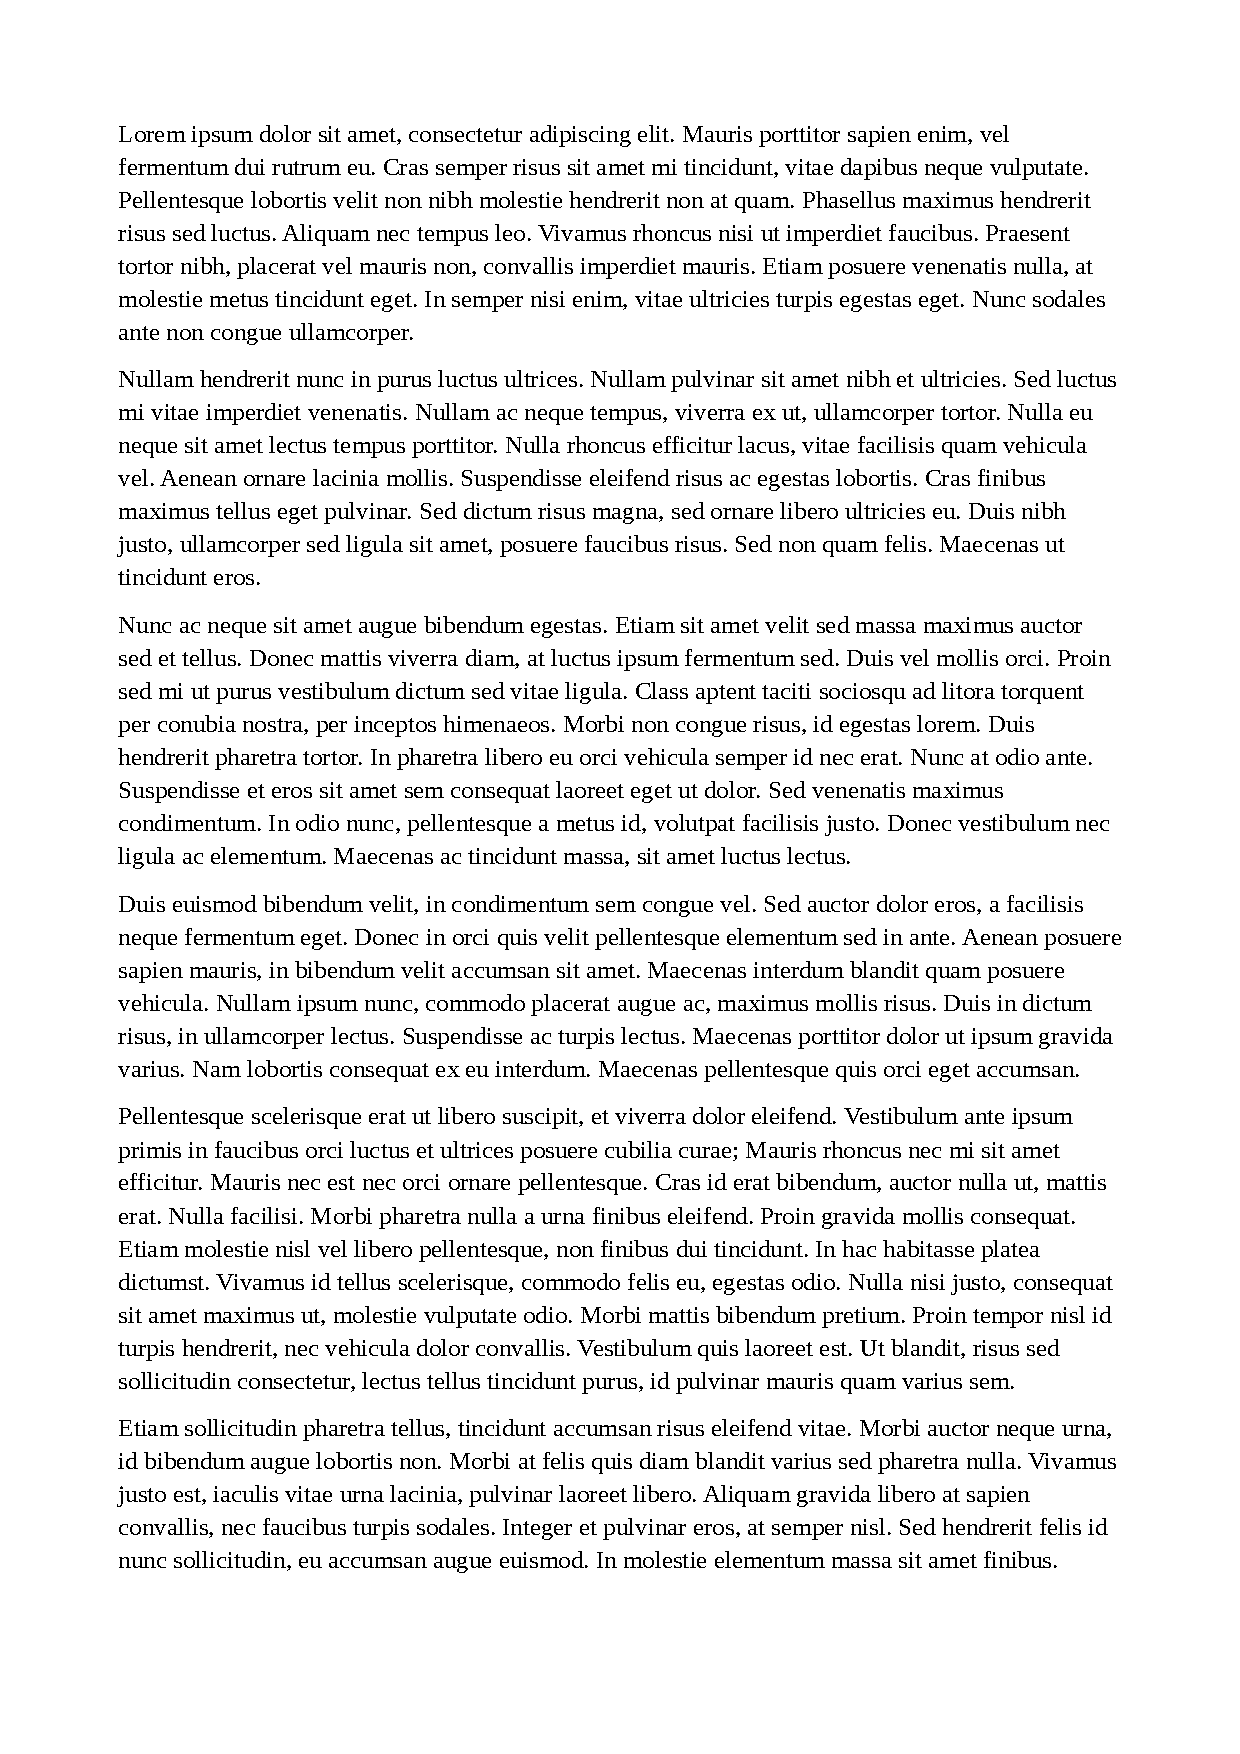
\includepdf[pages={1},scale=0.8,pagecommand=\chapter{Texto Texto Texto Texto}\label{apen:apendiceA}]{appendix/apendiceA}
% \includepdf[pages={2-},scale=0.80,pagecommand={}]{appendix/apendiceA}

\chapter{Socioeconomic Questionnaire}
\label{chap:socio-quest}

\begin{table}[ht]
\caption{Socioeconomic Questionnaire (Part I).}
\label{tbl:socioeconomic-questionnaire-part-i}
\centering
\rowcolors{1}{}{lightgray}
\begin{tabular}{ 
    p{1cm}
    p{9.5cm}
    >{\centering\arraybackslash}m{2.5cm}}
\hline
\multicolumn{1}{c}{\textbf{\#}} & \multicolumn{1}{c}{\textbf{Question}} &
\multicolumn{1}{c}{\textbf{Type}} \\
\hline

1 & Name & Text\\
2 & Birthdate & Date\\
3 & Enrollment Number & Text\\
4 & Semester of Admission & Text\\
5 & Sex Assigned at Birth:
\begin{enumerate}[label=(\alph*)]
    \item Male
    \item Female
    \item Intersex
    \item Prefer not do disclose
\end{enumerate} &
Multiple- choice\\
6 & Gender Identity & Text\\
7 & Sexual Orientation & Text\\
8 & Race/Ethnicity:
\begin{enumerate}[label=(\alph*)]
    \item White
    \item Yellow
    \item Brown
    \item Black
    \item Indigenous
    \item Other:\_\_\_
\end{enumerate} &
Text \\

\hline



\end{tabular}

  \par\medskip\ABNTEXfontereduzida\selectfont\textbf{Source:} Created by the author (2024). \par\medskip
\end{table}

\begin{table}[ht]
\caption{Socioeconomic Questionnaire (Part II).}
\label{tbl:socioeconomic-questionnaire-part-ii}
\centering
\rowcolors{1}{}{lightgray}
\begin{tabular}{ 
    p{1cm}
    p{9.5cm}
    >{\centering\arraybackslash}m{2.5cm}}
\hline
\multicolumn{1}{c}{\textbf{\#}} & \multicolumn{1}{c}{\textbf{Question}} &
\multicolumn{1}{c}{\textbf{Type}} \\
\hline

9 & How many people are in your family? & Numerical \\
10 & What is your mother’s scholarship? 
\begin{enumerate}[label=(\alph*)]
    \item Never studied or did not complete the 5th grade.
    \item Completed the 5th grade.
    \item Completed the 9th grade.
    \item Completed the 12th grade (high school).
    \item Completed university graduate.
\end{enumerate} &
Multiple- choice\\
11 & What is the total income of your family?
\begin{enumerate}[label=(\alph*)]
    \item Less than 2 minimum wages.
    \item Between 2 and 3 minimum wages.
    \item Between 3 and 5 minimum wages.
    \item Between 5 and 10 minimum wages.
    \item More than 10 minimum wages.
\end{enumerate} &
Multiple- choice\\


\hline



\end{tabular}

  \par\medskip\ABNTEXfontereduzida\selectfont\textbf{Source:} Created by the author (2024). \par\medskip
\end{table}
\chapter{Semi-Structured Scripts}
\label{chap:appendix-scripts}

\begin{table}[ht]
\caption{Semi-structured script for interviews: Motivations and Aspirations.}
\label{tbl:motivation-aspiration-script}
\centering
\rowcolors{1}{}{lightgray}
\begin{tabular}{p{1cm}p{12.5cm}}
\hline
\multicolumn{1}{c}{\textbf{\#}} & \multicolumn{1}{c}{\textbf{Reference Question}}\\
\multicolumn{1}{c}{IQ.1} &
What led you to do this undergraduate program?\\
\multicolumn{1}{c}{IQ.2} &
Was there something you expected about the program that changed after you entered?
\begin{enumerate}
    \item[(a)] And what did match your expectations?
\end{enumerate}\\
\multicolumn{1}{c}{IQ.3} &
How do you imagine yourself after graduating?\\
\multicolumn{1}{c}{IQ.4} &
What led you to choose \gls{UFPE}? 
Would you do your undergraduate program in another place?\\
\multicolumn{1}{c}{IQ.5} &
Tell me a bit more about your weekly routine:
\begin{enumerate}
    \item[(a)] How is it your common day during the week?
    \item[(b)] How are your weekends usually?
    \item[(c)] How are your holidays usually? 
\end{enumerate}\\
\hline

\end{tabular}

  \par\medskip\ABNTEXfontereduzida\selectfont\textbf{Source:} Created by the author (2024). \par\medskip
\end{table}

\begin{table}[ht]
\caption{Semi-structured script for interviews: Self-Directed Learning (Part I).}
\label{tbl:sdl-script-part-i}
\centering
\rowcolors{1}{}{lightgray}
\begin{tabular}{
    p{1cm}
    p{9.5cm}
    p{2.5cm}
}
\hline

\multicolumn{1}{c}{\textbf{\#}} & \multicolumn{1}{c}{\textbf{Reference Question}} & \multicolumn{1}{c}{\textbf{Construct}}\\

\multicolumn{1}{c}{IQ.6} &
Do you use any approach or strategy when you need to study for your own account?
\begin{enumerate}
    \item[(a)] If yes, what?
    \item[(b)] Could you describe it for me in more detail?
\end{enumerate} &
needs, goals, strategy\\

\multicolumn{1}{c}{IQ.7} &
What do you do when you need to learn anything that is required in the course? &
needs, goals, strategy\\

\multicolumn{1}{c}{IQ.8} &
Who do you consult (or talk to) when you need to clear your doubts or deepen your understanding of anything? &
resources (people)\\

\multicolumn{1}{c}{IQ.9} &
Do you like to work in a group?
\begin{enumerate}
    \item[(a)] If no, why?
\end{enumerate} &
resources (people)\\


\hline

\end{tabular}

  \par\medskip\ABNTEXfontereduzida\selectfont\textbf{Source:} Created by the author (2024). \par\medskip
\end{table}

\begin{table}[ht]
\caption{Semi-structured script for interviews: Self-Directed Learning (Part II).}
\label{tbl:sdl-script-part-ii}
\centering
\rowcolors{1}{}{lightgray}
\begin{tabular}{
    p{1cm}
    p{9.5cm}
    p{2.5cm}
}
\hline

\multicolumn{1}{c}{\textbf{\#}} & \multicolumn{1}{c}{\textbf{Reference Question}} & \multicolumn{1}{c}{\textbf{Construct}}\\

\multicolumn{1}{c}{IQ.10} &
What do you consult (or use) when you need to clear your doubts or deepen your understanding of anything? &
resources (objects)\\

\multicolumn{1}{c}{IQ.11} &
Where do you like to study when you need to study for your own account?
\begin{enumerate}
    \item[(a)] Is it possible to study in these places?
    \item[(b)]  Do you like to study at university?
    \item[(c)] Do you like to study at home?
\end{enumerate} &
resources (places)\\

\multicolumn{1}{c}{IQ.12} &
In addition to studying, do you have a job?
\begin{enumerate}
    \item[(a)] If yes, what?
    \item[(b)]  How much time does it occupy in your weekly schedule?
    \item[(c)] To guarantee your studying, is it essential you work?
\end{enumerate} &
resources (time)\\

\multicolumn{1}{c}{IQ.13} &
When you study for your own account, is there anything you want but you can not do?
\begin{enumerate}
    \item[(a)] If yes, what?
    \item[(b)] Could you describe for me how you feel in these moments?
    \item[(c)] What do you do when you are in this situation?
\end{enumerate} &
capability, resource\\

\multicolumn{1}{c}{IQ.14} &
How do you know if you are in the right way (or not) when you study for your own account?
\begin{enumerate}
    \item[(a)] What do you do when you realize that something is wrong?
\end{enumerate} &
evaluation\\

\hline

\end{tabular}

  \par\medskip\ABNTEXfontereduzida\selectfont\textbf{Source:} Created by the author (2024). \par\medskip
\end{table}


\begin{landscape}

\chapter{Data Charting}
\label{chap:data-charting}

    \begin{table}[htb]
\caption{Charting of the selected papers after the first two iterations of the snowballing process (Papers 1-5).}
\label{tbl:papers-chart}
\centering
\rowcolors{1}{}{lightgray}
\begin{tabular}{
    >{\centering\arraybackslash}m{2cm}|
    >{\centering\arraybackslash}m{2cm}|
    >{\centering\arraybackslash}m{2cm}|
    >{\centering\arraybackslash}m{2.5cm}|
    >{\centering\arraybackslash}m{2.2cm}|
    >{\centering\arraybackslash}m{2cm}|
    >{\centering\arraybackslash}m{2cm}|
    >{\centering\arraybackslash}m{2cm}|
    >{\centering\arraybackslash}m{2.5cm}
}
    \hline
    %\multicolumn{2}{c}{Item of Information} &
    & 
    \multicolumn{3}{c|}{
        \textbf{Research}
    } &
    \multicolumn{2}{c|}{
        \textbf{Context}
    } &
    \multicolumn{2}{c|}{
        \textbf{Equity} 
    } &    
    \textbf{Active Learning} \\
    \hline
    
    \textbf{Paper} &
    \textbf{Type} &
    \textbf{Kind} &
    \textbf{Methodology} &
    \textbf{Educational Level} &
    \textbf{Country} &
    \textbf{Equity Issue} &
    \textbf{General Equity Theory / Framework} &
    \textbf{Approach }\\    
    \hline 

    \cite{akalin:2021} &
    Research Project &	
    Primary &
    - &	
    Higher Education &	
    USA (?) &
    Gender &	
    - &	
    Pair Programming \\
    \hline

    \cite{alvarado:2022} &	
    Report &	
    Primary &	
    Program Evaluation &	
    Higher Education &	
    USA &	
    Gender, Race &	
    - &	
    Dual-Mentoring \\
    \hline

    \cite{arawjo:2021} &	
    Research &	
    Primary &	
    Ethnography &	
    Informal Educational, 6th grade &	
    East Africa, USA &	
    Culture, Refugee, Gender, Race &	
    Intercultural Computing &	
    Pair Programming \\
    \hline

    \cite{ayub:2020} &	
    Report &	
    Primary &	
    Program Evaluation &	
    Higher Education &	
    Indonesia &	
    Slow-pacing &	
    - &	
    Pair Programming \\
    \hline
    
    \cite{bodaker:2023} &	
    Research &	
    Primary &	
    Mixed-methods &	
    4th-6th grades &	
    Israel (?) &	
    Gender &	
    Gender Gap &	
    Pair Programming \\
    \hline
    
\end{tabular}

\par\medskip\ABNTEXfontereduzida\selectfont\textbf{Source:} Created by the author (2024). \par\medskip

\end{table}

\end{landscape}

%=====================
%PART II - 6 TO 10
%=====================

\begin{landscape}

    \begin{table}[htb]
\caption{Charting of the selected papers after the first two iterations of the snowballing process (Papers 6-10).}
\label{tbl:papers-chart}
\centering
\rowcolors{1}{}{lightgray}
\begin{tabular}{
    >{\centering\arraybackslash}m{2cm}|
    >{\centering\arraybackslash}m{2cm}|
    >{\centering\arraybackslash}m{2cm}|
    >{\centering\arraybackslash}m{2.5cm}|
    >{\centering\arraybackslash}m{2.2cm}|
    >{\centering\arraybackslash}m{2cm}|
    >{\centering\arraybackslash}m{2cm}|
    >{\centering\arraybackslash}m{2cm}|
    >{\centering\arraybackslash}m{2.5cm}
}
    \hline
    %\multicolumn{2}{c}{Item of Information} &
    & 
    \multicolumn{3}{c|}{
        \textbf{Research}
    } &
    \multicolumn{2}{c|}{
        \textbf{Context}
    } &
    \multicolumn{2}{c|}{
        \textbf{Equity} 
    } &    
    \textbf{Active Learning} \\
    \hline
    
    \textbf{Paper} &
    \textbf{Type} &
    \textbf{Kind} &
    \textbf{Methodology} &
    \textbf{Educational Level} &
    \textbf{Country} &
    \textbf{Equity Issue} &
    \textbf{General Equity Theory / Framework} &
    \textbf{Approach }\\    
    \hline 

    \cite{bowman:2020} &	
    Research &	
    Primary &	
    Survey &	
    Higher Education &	
    USA &	
    Nationality &	
    - &	
    Pair Programming \\
    \hline

    \cite{broll:2021} &
    Research &	
    Primary	&
    Multiple Evaluation Study &	
    Informal, Basic, and Higher Education &	
    USA (?) &	
    Access &	
    - &	
    Project-Based Learning, Pair Programming \\
    \hline

    \cite{demir:2021} &
    Research &	
    Primary &	
    Mixed-methods &	
    Higher Education &	
    Turkey &	
    Gender, Personality Traits, Learning Style, Friendship, Prior Knowledge &	
    - &	
    Pair Programming \\
    \hline

    \cite{eglash:2020} &	
    Research &	
    Primary &	
    Survey &	
    High School &	
    USA &	
    Native Community &	
    - &	
    Mixed Approaches \\
    \hline
    
    \cite{goode:2021} &	
    Research &	
    Primary &	
    Mixed-methods &	
    Professional Education &	
    USA (?) &	
    Race &	
    - &	
    Mixed Approaches \\
    \hline
    
\end{tabular}

\par\medskip\ABNTEXfontereduzida\selectfont\textbf{Source:} Created by the author (2024). \par\medskip

\end{table}

\end{landscape}

%=====================
%PART III - 11 TO 15
%=====================

\begin{landscape}

    \begin{table}[htb]
\caption{Charting of the selected papers after the first two iterations of the snowballing process (Papers 11-15).}
\label{tbl:papers-chart}
\centering
\rowcolors{1}{}{lightgray}
\begin{tabular}{
    >{\centering\arraybackslash}m{2cm}|
    >{\centering\arraybackslash}m{2cm}|
    >{\centering\arraybackslash}m{2cm}|
    >{\centering\arraybackslash}m{2.5cm}|
    >{\centering\arraybackslash}m{2.2cm}|
    >{\centering\arraybackslash}m{2cm}|
    >{\centering\arraybackslash}m{2cm}|
    >{\centering\arraybackslash}m{2cm}|
    >{\centering\arraybackslash}m{2.5cm}
}
    \hline
    %\multicolumn{2}{c}{Item of Information} &
    & 
    \multicolumn{3}{c|}{
        \textbf{Research}
    } &
    \multicolumn{2}{c|}{
        \textbf{Context}
    } &
    \multicolumn{2}{c|}{
        \textbf{Equity} 
    } &    
    \textbf{Active Learning} \\
    \hline
    
    \textbf{Paper} &
    \textbf{Type} &
    \textbf{Kind} &
    \textbf{Methodology} &
    \textbf{Educational Level} &
    \textbf{Country} &
    \textbf{Equity Issue} &
    \textbf{General Equity Theory / Framework} &
    \textbf{Approach }\\    
    \hline 

    \cite{grabl:2024} &	
    Research &	
    Primary	&
    Survey	&
    Higher Education, Secondary School	&
    Germany (?)	&
    Dominance	&
    -	&
    Pair Programming \\
    \hline

    \cite{gransbury:2022} &
    Research Project	&
    Primary	&
    Mixed-methods &
    K-12 &	
    USA (?) &	
    Gender	&
    -	&
    Pair Programming \\
    \hline
    
    \cite{izhikevich:2022} &
    Research &
    Primary &
    Mixed-methods &
    Higher Education &
    USA &
    Sense of belonging &
    - &
    Pair Programming \\
    \hline
    
    \cite{kung:2022} &
    Research &
    Primary &
    Descriptive Quantitative Research & 
    K-12 &
    Switzerland &
    Gender &
    - &
    Pair Programming \\
    \hline

    \cite{lai:2023} &
    Systematic Review &
    Secondary &
    \cite{kitchenham:2007} &
    - &	
    - &	
    Social Cognitive Factors &	
    - &	
    Collaborative Learning \\
    \hline
    
\end{tabular}

\par\medskip\ABNTEXfontereduzida\selectfont\textbf{Source:} Created by the author (2024). \par\medskip

\end{table}

\end{landscape}

%=====================
%PART IV - 16 TO 21
%=====================

\begin{landscape}

    \begin{table}[htb]
\caption{Charting of the selected papers after the first two iterations of the snowballing process (Papers 16-21).}
\label{tbl:papers-chart}
\centering
\rowcolors{1}{}{lightgray}
\begin{tabular}{
    >{\centering\arraybackslash}m{2cm}|
    >{\centering\arraybackslash}m{2cm}|
    >{\centering\arraybackslash}m{2cm}|
    >{\centering\arraybackslash}m{2.5cm}|
    >{\centering\arraybackslash}m{2.2cm}|
    >{\centering\arraybackslash}m{2cm}|
    >{\centering\arraybackslash}m{2cm}|
    >{\centering\arraybackslash}m{2cm}|
    >{\centering\arraybackslash}m{2.5cm}
}
    \hline
    %\multicolumn{2}{c}{Item of Information} &
    & 
    \multicolumn{3}{c|}{
        \textbf{Research}
    } &
    \multicolumn{2}{c|}{
        \textbf{Context}
    } &
    \multicolumn{2}{c|}{
        \textbf{Equity} 
    } &    
    \textbf{Active Learning} \\
    \hline
    
    \textbf{Paper} &
    \textbf{Type} &
    \textbf{Kind} &
    \textbf{Methodology} &
    \textbf{Educational Level} &
    \textbf{Country} &
    \textbf{Equity Issue} &
    \textbf{General Equity Theory / Framework} &
    \textbf{Approach }\\    
    \hline 

    \cite{lott:2021} &
    Research &
    Primary &
    Mixed-methods &
    - &	
    - &	
    Gender &	
    - &	
    Pair Programming \\
    \hline
    
    \cite{love:2021} &
    Research &
    Primary	&
    Interaction Analysis, Positioning Theory	&
    ??? &	
    USA (?) &	
    Race &	
    Epistemic Injustice &	
    Pair Programming \\
    \hline
    
    \cite{lui:2020} &
    Research &	
    Primary &	
    Qualitative Research &	
    High School &	
    USA (?) &	
    Gender (?), Expertise &	
    - &	
    Pair Physical Computing \\
    \hline

    \cite{lyttle:2020} &
    Report	&
    Primary	&
    Program Evaluation	&
    High School	&
    USA (?)	&
    Novice learners	&
    -	&
    Pair Programming \\
    \hline

    \cite{michaelis:2022} &
    Essay	&
    Primary	&
    -	&
    -	&
    -	&
    Interest, Sense of Belonging &
    Interest Development Theory	&
    Problem-based Learning \\
    \hline

    \cite{musaeus:2022} &
    Research	&
    Primary	&
    Pilot Study	&
    High School	&
    Denmark	&
    Online Participation	&
    -	&
    Collaborative Learning \\
    \hline
    
\end{tabular}

\par\medskip\ABNTEXfontereduzida\selectfont\textbf{Source:} Created by the author (2024). \par\medskip

\end{table}

\end{landscape}

%=====================
%PART V - 22 TO 26
%=====================

\begin{landscape}

    \begin{table}[htb]
\caption{Charting of the selected papers after the first two iterations of the snowballing process (Papers 22-26).}
\label{tbl:papers-chart}
\centering
\rowcolors{1}{}{lightgray}
\begin{tabular}{
    >{\centering\arraybackslash}m{2cm}|
    >{\centering\arraybackslash}m{2cm}|
    >{\centering\arraybackslash}m{2cm}|
    >{\centering\arraybackslash}m{2.5cm}|
    >{\centering\arraybackslash}m{2.2cm}|
    >{\centering\arraybackslash}m{2cm}|
    >{\centering\arraybackslash}m{2.2cm}|
    >{\centering\arraybackslash}m{2cm}|
    >{\centering\arraybackslash}m{2.5cm}
}
    \hline
    %\multicolumn{2}{c}{Item of Information} &
    & 
    \multicolumn{3}{c|}{
        \textbf{Research}
    } &
    \multicolumn{2}{c|}{
        \textbf{Context}
    } &
    \multicolumn{2}{c|}{
        \textbf{Equity} 
    } &    
    \textbf{Active Learning} \\
    \hline
    
    \textbf{Paper} &
    \textbf{Type} &
    \textbf{Kind} &
    \textbf{Methodology} &
    \textbf{Educational Level} &
    \textbf{Country} &
    \textbf{Equity Issue} &
    \textbf{General Equity Theory / Framework} &
    \textbf{Approach }\\    
    \hline 

    \cite{nakai:2023} &	
    Research &	
    Primary &	
    Mixed-methods &	
    Higher Education &	
    USA &	
    Self-efficacy &	
    - &	
    Peer-mentoring guide \\
    \hline

    \cite{roque-hernandez:2021} & 
    Research &	
    Primary	&
    Experimental Research &	
    Higher Education &	
    Mexico &	
    Gender, Expertise &	
    - &	
    Pair Programming \\
    \hline
    
    \cite{shahin:2022} &
    Research &	
    Primary	&
    Mixed-methods &	
    High School	&
    Australia &	
    Gender	&
    - &	
    Problem-based Learning \\
    \hline

    \cite{su:2023} &	
    Research &	
    Primary	&
    Epistemic Network Analysis &	
    5th grade &	
    China (?) &	
    Performance &	
    - &	
    Pair Programming \\
    \hline

    \cite{tan:2024} &	
    Research &
    Primary	&
    Experimental Research &	
    Third Education &	
    China &	
    Self-efficacy &	
    -	&
    Pair Programming \\
    \hline
    
\end{tabular}

\par\medskip\ABNTEXfontereduzida\selectfont\textbf{Source:} Created by the author (2024). \par\medskip

\end{table}

\end{landscape}

%=====================
%PART VI - 27 TO 31
%=====================

\begin{landscape}

    \begin{table}[htb]
\caption{Charting of the selected papers after the first two iterations of the snowballing process (Papers 27-31).}
\label{tbl:papers-chart}
\centering
\rowcolors{1}{}{lightgray}
\begin{tabular}{
    >{\centering\arraybackslash}m{2cm}|
    >{\centering\arraybackslash}m{2cm}|
    >{\centering\arraybackslash}m{2cm}|
    >{\centering\arraybackslash}m{2.5cm}|
    >{\centering\arraybackslash}m{2.2cm}|
    >{\centering\arraybackslash}m{2cm}|
    >{\centering\arraybackslash}m{2.2cm}|
    >{\centering\arraybackslash}m{2cm}|
    >{\centering\arraybackslash}m{2.5cm}
}
    \hline
    %\multicolumn{2}{c}{Item of Information} &
    & 
    \multicolumn{3}{c|}{
        \textbf{Research}
    } &
    \multicolumn{2}{c|}{
        \textbf{Context}
    } &
    \multicolumn{2}{c|}{
        \textbf{Equity} 
    } &    
    \textbf{Active Learning} \\
    \hline
    
    \textbf{Paper} &
    \textbf{Type} &
    \textbf{Kind} &
    \textbf{Methodology} &
    \textbf{Educational Level} &
    \textbf{Country} &
    \textbf{Equity Issue} &
    \textbf{General Equity Theory / Framework} &
    \textbf{Approach }\\    
    \hline 

    \cite{toro:2024} &
    Research &
    Primary	&
    Experimental Research &
    Higher Education &	
    Spain &	
    Gender	&
    -	&
    Pair Programming \\
    \hline

    \cite{tseng:2024} &
    Research &
    Primary	&
    Mixed-methods &
    Informal Education &
    USA (?) &
    Data Diversity &
    - &
    Collaborative Learning \\
    \hline

    \cite{wei:2021} &	
    Research &	
    Primary	&
    Mixed-methods &	
    K-12 &	
    China &	
    Self-efficacy &	
    - &	
    Partial Pair Programming \\
    \hline

    \cite{ying:2021} &
    Research &	
    Primary	 &
    Experimental Research &	
    Higher Education &	
    USA	&
    Gender &	
    - &	
    Pair Programming \\
    \hline
    
    \cite{ying:2021b} &	
    Research &	
    Primary	&
    Experimental Research &	
    Higher Education &	
    USA	&
    Gender &	
    - &	
    Collaborative Learning \\
    \hline
    
\end{tabular}

\par\medskip\ABNTEXfontereduzida\selectfont\textbf{Source:} Created by the author (2024). \par\medskip

\end{table}

\end{landscape}
\chapter{Interview Excerpts}
\label{chap:interview-excerpts}

This section presents the interview excerpts in Brazilian Portuguese (in their original transcript before translation). The excerpts used in this work (see Section \ref{chap:results}) were translated to English for a better reading flux. Section \ref{interview-exc-sec:chavo} refers to Chavo’s interview excerpts, and Section \ref{interview-exc-sec:quico} to Quico’s ones. 

\section{Chavo’s Interview Excerpts}
\label{interview-exc-sec:chavo}

The original Chavo's answers in Brazilian Portuguese concerning 
% \gls{IQ}.1, 
\gls{IQ}.2, 
\gls{IQ}.3, 
% \gls{IQ}.4, 
\gls{IQ}.5, 
\gls{IQ}.6, 
%\gls{IQ}.7, 
\gls{IQ}.8, 
\gls{IQ}.9, 
\gls{IQ}.10, 
\gls{IQ}.11,   
\gls{IQ}.12, and 
\gls{IQ}.13
% \gls{IQ}.14 
questions are presented as follows. The other answers have not been explored in an appropriate way yet.

% \subsection{Chavo’s IQ.1 answer}
% \label{interview-exc-ss:chavo-iq1}

\subsection{Chavo’s IQ.2 answer}
\label{interview-exc-ss:chavo-iq2}

\begin{quote}
    \itshape
    "Eu acho que eu tive muita expectativa com administração. Eu sabia que tinha, mas não sabia muito como era... eu nunca tinha visto muito. A parte de programação eu já tinha estudado um pouco antes, já tinha vivido um pouco antes. Então eu já sabia um pouco o que iria acontecer. Mas, tipo... me chamou muito a atenção, porque eu esperava que, tipo... eu não sei como é a administração, eu sei que vai ter questão de gerenciar alguma coisa de projeto, ciclo de vida de projeto em alguma cadeira, mas não sabia como seria. Aí que eu iria ter que estudar, tipo... os primórdios da administração, administração científica, essas coisas, sabe? Aí isso mudou muito".

    \colorbox{black!15}{Eu: Sim. Aí tu não tinha percepção clara e isso aí veio durante o curso?}

    "Isso". 
\end{quote}

\subsection{Chavo’s IQ.3 answer}
\label{interview-exc-ss:chavo-iq3}

\begin{quote}
    \itshape
    "Hoje mudou muita coisa. Eu pretendo muito me aprofundar na parte tanto de programação, sim..., mas também na parte de nuvem, que é algo que eu estou vendo mais agora e eu me interessei bastante. Sempre me interessei pela parte de segurança. Então [essas] são [algumas] das áreas que eu gosto muito... e programação. Eu sempre gostei de programação. E a minha expectativa é tentar correr atrás para tentar me desenvolver: virar [desenvolvedor] júnior, pleno, sênior, e conseguir me aprofundar nessas áreas que eu gosto para tentar ser um dos especialistas no mercado, ser referência. Acho que a gente sempre quer ser referência no que a gente gosta".

    \colorbox{black!15}{Eu: Sim, lógico. E aí, bom... a partir da resposta que você deu aí, tem principal-} \colorbox{black!15}{mente na área de SI... tem esses dilemas daquele que 'coda' e aquele que gere, e} \colorbox{black!15}{tem os que são híbridos: os que curte tanto um quanto outro. Mas, assim... você} \colorbox{black!15}{tem afinidades mais técnicas? Como é que você se enxerga assim nesse universo} \colorbox{black!15}{aí? Porque você tem competências mil aí... em jogo aí no curso de SI [Sistemas} \colorbox{black!15}{de Informação]. Como é que você enxerga esse negócio aí?}

    "Então, eu nunca fui... Foi um pouco mais difícil para mim a parte de gestão. Eu estou conseguindo melhorar bastante e agora, principalmente agora na cadeira. Me perdi um pouco, mas agora estou voltando... estou pegando a manha de como que realmente a gente faz para conseguir gerir as coisas direitinho. Acho que a parte técnica sempre foi algo que já era mais fácil para mim, porque como eu já tinha estudado um pouco de robótica antes, no ensino médio, algo que me ajudou muito, então a parte técnica foi muito boa. Aí a parte de gerenciar está vindo mais agora. Agora que eu estou conseguindo melhorar ela".      
\end{quote}

% \subsection{Chavo’s IQ.4 answer}
% \label{interview-exc-ss:chavo-iq4}

\subsection{Chavo’s IQ.5 answer}
\label{interview-exc-ss:chavo-iq5}

\begin{quote}
    \itshape
    "Sim. Geralmente, a minha semana... Foi uma loucura também o que aconteceu. Porque eu preenchi o formulário, quando eu coloquei só tinha eu e minha mãe, e aí eu consegui entrar agora em uma empresa de tecnologia. Aí agora já mudou os dados do formulário. Mas está tranquilo. 
    
    Aí, tipo... agora eu trabalho. Acordo de 06h00, 06h20 mais ou menos. Aí eu fico até... assim... descanso um pouquinho, estudo, tomo café. Aí entre as 06h00 e as 10h00. 10h00 eu começo a trabalhar. Aí para de meio-dia, volto 01h00. Aí de 01h00 até 04h00, que é o estágio que eu consegui com a Federal, aí são 6 horas.

    Aí quando termina às 04h00, eu largo, eu me arrumo literalmente. É um pouquinho corrido, mas tranquilo. Eu me arrumo... aí eu tenho duas opções: ou eu vou andando, porque é perto, aí dá para ir andando tranquilo, gasta mais ou menos uns 20, 25 minutinhos.

    \colorbox{black!15}{Eu: Pertinho.}
    
    É um tempinho. Ou eu pego o ônibus. Só que o ônibus ele passa de 04h20. Aí tem a correria de se arrumar, torcer para ele passar às  04h25 ou 04h20, mas dá para pegar tranquilo. 
    
    Aí geralmente é isso. Tenho aula da faculdade. Quando largo, pego o ônibus no CCN [Centro de Ciências Exatas e Naturais] e vou para casa. Aí eu só reviso as coisas e vou dormir... comer e dormir.
    
    A semana é mais ou menos assim. Final de semana eu só olho mais para ver as coisas da faculdade e organizar um pouco as coisas da semana... ver se tem algum compromisso, se precisa ir para a empresa ou se precisa ir para a faculdade para estudar mais... essas coisas. E aproveitar. De resto, é mais isso.

    
    \colorbox{black!15}{Eu: E aí perguntar a tu, o estágio que tu está agora, tu entrou agora recente? \ } \colorbox{black!15}{Faz quanto tempo que tu entrou?}
    
    Eu acho que faz mais ou menos umas duas semaninhas, acho que no máximo. Essa eu acho que vai fazer duas semanas, eu acho. Faz pouquíssimo tempo que eu entrei.

    \colorbox{black!15}{Eu: Massa. Beleza. Depois a gente volta para essa parte do... Beleza? Legal?}
    
    Tranquilo.
    
    \colorbox{black!15}{Eu: E aí deixa eu te perguntar. Nesse trânsito aí... nesse processo aí... de tu sair} \colorbox{black!15}{de um lugar para o outro. Como é que gere a alimentação, comida? Como tu faz} \colorbox{black!15}{esse processo aí?}
    
    Geralmente, eu e a minha mãe, a gente geralmente divide. Às vezes, ela faz o almoço. Quando ela está sem tempo, eu desenrolo. Aí a gente deixa na geladeira. Eu sempre deixo separado a marmita às vezes. Quando eu preciso ir para a faculdade, ir para o trabalho... já tem a comida separada. Aí quando eu sei que vou ficar em casa, só deixo a comida congelada ali. Chegou a hora do almoço, esquentar... está tranquilo. 
    
    Agora, o lanche... ou eu pego algumas coisas e levo... em casa, tipo macarrão, carne, alguma coisa assim. Ou eu compro um salgado perto do \gls{CIn}. Geralmente eu faço muito isso... é mais prático".
\end{quote}

\subsection{Chavo’s IQ.6 answer}
\label{interview-exc-ss:chavo-iq6}

\begin{quote}
    \itshape
    “Quando é algo que eu não sei realmente do que eu estou vendo, primeiro eu pesquiso na internet, tento buscar mais a fundo se tem documentação. Eu gosto muito de olhar documentação ou pesquisar vídeo no Youtube. E também tem bastante coisa, tem muito material bom na internet. Aí eu, primeiro, foco nessas duas coisas. Aí tento achar e entender como é que aquilo funciona.

    Eu faço meio que assim: primeiro, eu vou tentar ler, vou tentar ver o que aquilo é, como funciona. Por exemplo, digamos que... por exemplo, passe alguma coisa relacionado a Banco de Dados. Aí agora a cadeira de Banco de Dados, aí ele tem lá… está dando um tópico de Banco de Dados Conceitual. Eu não sei o que é conceitual: eu pesquiso na internet, eu procuro nos sites que eu mais conheço relacionados a tecnologia. Como tem muitos sites que aparecem de Linux, tem o do Tech, tem no Youtube também. Aí eu pesquiso, tento estudar, aprender. Aí depois que eu aprendo, eu geralmente eu vejo os pontos, eu coloco meio é… um bloquinho com os pontos, assim, que eu aprendi, que eu coloco no computador. Ou se o professor já disponibilizar um exemplo, o assunto, aí eu assisto pelo do professor e depois eu pesquiso na internet para tentar dar uma revisada também. Eu faço meio que uma mistura dos dois.

    \colorbox{black!15}{Eu: Massa, beleza. [...]. Então, você está em uma disciplina... está dentro da fa-} 
    \colorbox{black!15}{culdade. E aí o professor te exige algo. E aí existe alguma coisa diferente que tu} 
    \colorbox{black!15}{faz porque é um assunto de faculdade ou a estratégia segue mais ou menos a } \mbox{    } \colorbox{black!15}{mesma linha?}

    Depende. Depende também do escopo que ele passa para a gente. Porque, por exemplo, na cadeira de Contabilidade, o professor passou para gente uma coisa que ele nunca tinha passado para o pessoal, que era relacionado a fazer meio que uma "aplicação" utilizando coisas gerenciais. Então, tipo... para mim, foi algo que ele não tinha passado material e que, nessa cadeira, eu tive que pesquisar por conta própria. Aí eu tive que utilizar um método diferente. Então, tipo... a partir do escopo que ele me deu, eu fui pesquisando os pontos. Aí, como é que eu poderia... por exemplo, utilizando o Python, como é que eu poderia criar uma aplicação? Aí eu pesquisei, sabe? Como ferramentas ou bibliotecas para auxiliar na criação de telas... realmente uma aplicação em Python. Aí com isso eu conseguir levantar o tópico de... tipo... qual seria a melhor para utilizar em questão do tempo do projeto, se o projeto tivesse muito apertado,  muito grande... [ou] se eu poderia utilizar uma simples ou uma mais completa. Aí, geralmente, eu utilizo esse ponto e, depois disso, depois de estudar qual o melhor ponto, eu entro mais a fundo com o tema que o professor passou. Tipo... primeiro, eu vejo geralmente os requisitos. No caso... nesse caso, acho que seriam os requisitos e depois eu vejo direitinho a parte mais profundamente para planejar quando que eu vou começar a fazer ou já começar a fazer direto". 
\end{quote}

% \subsection{Chavo’s IQ.7 answer}
% \label{interview-exc-ss:chavo-iq7}

\subsection{Chavo’s IQ.8 answer}
\label{interview-exc-ss:chavo-iq8}

\begin{quote}
    \itshape
    "Eu tento entrar em contato com os meus amigos. Assim... os que eu mais convivo geralmente. Aí, geralmente, eu pergunto para eles: `Gente, vocês entenderam o que o professor pediu?' ou `Vocês entenderam tal assunto?'. Que a gente tem o grupinho da gente, aí eu pergunto para eles.

    Acho que são mais ou menos, assim... umas 7 pessoas, mais ou menos 8 pessoas. E aí eu tento falar com o pessoal. Se eu não consigo, ou se eu não entender, eu pergunto no outro grupo que tem do pessoal da sala, que é o do período que a gente entrou, que é um pessoal que a gente está mais familiarizado desde o primeiro período. Aí eu tento perguntar para eles. Aí peço ajuda ao pessoal e o pessoa ajuda e a gente está se entendendo. E é bom, porque se tiver mais alguma pessoa com dúvida, aí a gente até ajuda... vai um Discord, vai uma ligaçãozinha. Aí a gente desenrola para conseguir entender o assunto. Geralmente, eu faço isso". 
\end{quote}

\subsection{Chavo’s IQ.9 answer}
\label{interview-exc-ss:chavo-iq9}

\begin{quote}
    \itshape
    "Sim. Eu sou muito tranquilo de trabalhar em grupo, consigo tranquilamente... eu consigo me adaptar. Qualquer grupo que você conseguir me colocar, assim... eu consigo me adaptar com o pessoal. Isso é uma coisa que para mim é de boa. Mas, assim... eu gosto muito de fazer trabalho com o pessoal que eu já tenho mais afinidade, porque fica mais tranquilo, porque o pessoal já conhece mais sobre mim, sobre a minha rotina também e eu conheço também do pessoal. Aí fica muito mais tranquilo, porque a gente já sabe, a gente conhece mais um ao outro, então sabe... tipo... `Ah, vamos fazer tal parte, outro faz tal parte'. A gente decide direitinho e fica melhor. Mas se não der, eu... Qualquer grupo, assim... com o pessoal, que me colocar, eu consigo desenrolar. Principalmente com o pessoal do período que a gente está, desde o primeiro. Eu tenho afinidade muito boa com todo mundo, então qualquer grupo é tranquilo".
\end{quote}

\subsection{Chavo’s IQ.10 answer}
\label{interview-exc-ss:chavo-iq10}

\begin{quote}
    \itshape
    "Eu já usei bastante a biblioteca física quando eu estava procurando livro de algoritmo. Porque livro de algoritmo? Como tinha muita coisa na internet, mas algumas coisas específicas você não encontrava na internet ou, tipo... só encontrava se você pesquisasse, por exemplo, em inglês. E fosse procurando bem muito e você conseguia achar. E tem outros que tinham em livro, aí eu achei mais fácil. Tipo... tem principalmente livros de referência, de algoritmos e estruturas de dados, acho que tem um que tem mil páginas, só que eu não lembro agora o autor, mas sei que tem tudo ali. Aí eu pegava ele. Via se tinha na biblioteca do CCEN [Centro de Ciências Exatas e da Natureza da \gls{UFPE}]. Se não tivesse, eu baixava ou... porque o livro é meio carinho. Aí eu dava uma desenrolada. 
    
    Mas eu gosto de usar o livro quando é um pouquinho mais difícil de encontrar na internet ou quando tem alguma coisa muito específica que o professor fala: 'Vocês não vão conseguir encontrar na internet' ou vai ser mais difícil de encontrar. Aí eu gosto de pegar um livro de referência aqui... já facilita mais as coisas.".    
\end{quote}
\subsection{Chavo’s IQ.11 answer}
\label{interview-exc-ss:chavo-iq11}

\begin{quote}
    \itshape
    "Bom, acho que tem sim dois lugares que eu mais gosto de estudar, no meu quarto principalmente. É porque geralmente eu fico mais por aqui, então como eu fico em casa a maior parte sozinho, eu já estou acostumado e não tem problema. Mas quando eu tenho que ir para a faculdade ou, por exemplo... ou no trabalho, no escritório... dá para conseguir trabalhar de boa, dar uma revisada de boa, mas na faculdade principalmente. 
    
    Eu estou fazendo muito isso essa semana. Vou fazer amanhã que amanhã vai ser corrido demais. E perto da gente, do [local de aulas de] SGE ali, que é do lado literalmente, tem uns banquinhos ali, tem tomada. Tipo... eu gosto de lá porque lá é ventilado e, mesmo com algumas pessoas, o pessoal respeita o silêncio.     É tranquilo de estudar por ali, ou então na biblioteca. Só que a biblioteca, como fica um pouco mais distante, eu prefiro já ficar pelo \gls{CIn} mesmo por causa do Wi-Fi.
    

    \colorbox{black!15}{Eu: Então você consegue fazer em casa algumas coisas. E tem algo que tu faz em}
    \colorbox{black!15}{casa e que não consegue fazer na faculdade, ou tem coisas que você na faculdade}
    \colorbox{black!15}{e que não consegue fazer em casa, em termos de estudo... Assim?}
    
    Acho que um pouco... é um pouco. É porque é um meio termo, não é? Porque, assim... em casa, às vezes, você procrastina um pouco. Isso acontece comigo relativamente sempre. Aí, tipo... na faculdade, eu consigo ter um foco maior, de verdade. Eu consigo me concentrar e ficar mais focado por mais tempo. Em casa, eu tenho algumas distrações, mas estou trabalhando para tentar melhorar. Mas acho que, em si, é mais isso. O ruim só é que, como eu ainda estou... o meu fone de ouvido BlueTooth está com a bateria ruim, eu estou esperando outro chegar, e está ruim de ver vídeo. Mas fora isso, na faculdade, quando eu estou sozinho, por exemplo, em um cantinho estudando... eu tenho um pouco mais de foco por mais tempo do que ficar em casa em si, porque como tem, por exemplo, WhatsApp e tem mensagem do pessoal, muitas coisas. Então eu estou em casa, é só levantar, ir ali e voltar. Mas, fora isso... acho que é mais isso mesmo".
\end{quote}
\subsection{Chavo’s IQ.12 answer}
\label{interview-exc-ss:chavo-iq12}

\begin{quote}
    \itshape
    "Entendo. Acho que não... pelo estudo... Eu consigo... dá para conseguir ficar com estudo e sem trabalhar, por causa que é Federal, mas é um pouquinho mais complicado. Porque como é só eu e mainha em casa... e antes de eu trabalhar ficava mais difícil por causa da passagem do ônibus e da comida na faculdade. E isso daí, porque... querendo ou não, passagem gasta bastante e comida também. Mas assim... eu acredito que seria mais isso. Mas é porque antes... Espera, eu acho que eu me... Espera aí. Tu pode repetir a pergunta, por favor? Porque eu me perdi". 

    \colorbox{black!15}{Eu: Posso. Eu estou falando o seguinte, se é essencial o seu trabalho pensando na} 
    \colorbox{black!15}{garantia do seu estudo.}

    "Entendi. Certo. Pronto... Seria mais a questão do transporte e um pouco da alimentação. Porque, assim, dá para conseguir ficar... dá. Só que você tem que realmente ser bem apertado. Por exemplo, antes de eu começar a fazer o estágio, o que é que eu fazia? Eu fazia muito assim... como a ida para a faculdade é tranquilo, ainda é de dia e tal... tudo certinho. Eu vou muitas vezes andando, porque é próximo, aí já economiza uma passagem. Eu só iria [de ônibus] na volta. Um exemplo, assim. Então é algo que você, assim... dá para conseguir desenrolar sem, mas fica bem mais complicado, sabe?".

    \colorbox{black!15}{Eu: E quando tu vem andando, tu vem com notebook, essas coisas ou não? Por-} \colorbox{black!15}{que também isso é um dilema.} 

    "Então, é... Então... eu não vinha. Muito difícil mesmo eu vir com notebook. Assim... eu tenho um amigo meu que mora próximo, daqui de $\langle$Acapulco$\rangle$. Aí ele vinha por aqui. Aí quando eu precisava de notebook ou precisava de carona, ele sempre me oferece. Aí quando eu estou indo com o notebook, alguma coisa assim, eu sempre ia com ele ou então eu pegava o busão. Mas quando ele me dava carona, tipo... já era melhor, que já ajudava". 
\end{quote}
\subsection{Chavo’s IQ.13 answer}
\label{interview-exc-ss:chavo-iq13}

\begin{quote}
    \itshape
    “Entendi. Isso já aconteceu comigo já no início, quando eu entrei no curso. No início, foi na cadeira de P1 [Programação Introdutória]. E pesou mais em algoritmos. Mas foi algoritmo, aí, que eu consegui construir uma fonte boa de lógica de programação. Que tinham algumas listas que… tipo... mesmo eu pesquisando, mesmo eu lendo a questão, eu não conseguia entender, porque eu ainda não tinha... eu não estava conseguindo entender realmente, como tu falou. Pelo ponto de falta de... que eu não conseguia. Aí quando eu não conseguia, eu pedia muito ajuda, eu pedia ajuda ao pessoal, principalmente do pessoal que eu já conhecia ou então o pessoal da sala que eu tinha conhecido na época. Aí eu pedia ajuda. O pessoal, sempre, tipo assim: "Ah, eu consigo te ajudar", tal pessoa, tipo… aí o pessoal explicar ou então eu pedia para entrar no Discord para ajudar, e eu pesquisava bastante. Então, tipo, eu ia dormir um pouquinho mais tarde, mas eu tentava pesquisar, tentava estudar de novo para entender melhor aquilo ali que eu não tinha conseguido”. 
\end{quote}
% \subsection{Chavo’s IQ.14 answer}
% \label{interview-exc-ss:chavo-iq14}

\section{Quico’s Interview Excerpts}
\label{interview-exc-sec:quico}

The original Quico's answers in Brazilian Portuguese concerning 
 \gls{IQ}.1, 
% \gls{IQ}.2, 
 \gls{IQ}.3, 
% \gls{IQ}.4, 
% \gls{IQ}.5, 
\gls{IQ}.6, 
%\gls{IQ}.7, 
\gls{IQ}.8, 
\gls{IQ}.9, 
\gls{IQ}.10, and 
\gls{IQ}.11  
% \gls{IQ}.12, 
% \gls{IQ}.13, 
% \gls{IQ}.14 
questions are presented as follows. The other answers have not been explored in an appropriate way yet.


 \subsection{Quico’s IQ.1 answer}
 \label{interview-exc-ss:quico-iq1}

 \begin{quote}
     \itshape
     "De começo, assim... eu tentei duas vezes o ENEM. A primeira [vez], infelizmente, não deu. A nota não foi suficiente. Aí a segunda, eu ainda estava com a mesma mentalidade de fazer Ciência da Computação. Só que aí vi que, pela nota, ali não ia rolar, e Sistemas da Informação a nota dava para entrar. 

    Aí a gente passou um tempo lá, eu e painho, conversando e tal. A gente via o histórico do SISU, as notas... como é que tinha ficado, se ia dar para entrar ou não. Aí, pela análise que a gente fez, Sistemas da Informação era um curso que estava dentro do que eu queria, que era relacionado a programação, e também dava para eu entrar.

    Então, assim... esse foi o principal motivo de eu ter escolhido Sistemas da Informação. Mais assim... por abordar o que eu queria e também estar dentro ali do que a nota permitia, entendeu? Então foi mais assim, foi esse motivo a escolha.

    \colorbox{black!15}{Eu: E essa parte de programação, tu já conhecia alguma coisa ou não? Ou tu era} \colorbox{black!15}{meio 'zerado'? Como é que era essa ideia?}

    Eu tinha uma base, assim... não tão grande, mas eu já tinha visto alguma coisa, sabe? Eu já tinha visto por fora, assim... no Youtube já tinha visto coisa relacionada a programação já. Eu foquei em uma lá, que era Python. E depois eu fiz um curso técnico no IF [Instituto Federal] de Paulista lá. Foi um ano e meio, fiz Manutenção e Suporte em Informática. Aí tinha também... tinha programação. Aí já fiquei com uma base maior. Teve esse período que eu fiquei aprendendo por fora, teve esse período do IF e agora o de Sistemas, não é? Então eu já tinha aí já um contexto, mesmo que simples, mas que já tinha já. 

    [...]

    \colorbox{black!15}{Eu: Que massa. Então, assim... tu fez o IF lá de Paulista e pelo menos essa ideia} \colorbox{black!15}{de diferenciar informática de Ciência da Computação tu tinha mais ou menos em} \colorbox{black!15}{mente? Ou não? Ou lá também não era tão claro assim?}

    É porque lá no do IF foi mais... foi um geralzão, entendeu? Pelo curso que eu fiz. Tinha Programação, aí tinha Redes, tinha Manutenção de Computadores, tinha Arquitetura de Computador, então era bem abrangente aquele curso. Aí a ideia de diferenciar de ciência assim para...

    \colorbox{black!15}{Eu: Diferença de maneira clara não tinha?}

    Não tinha não".
 \end{quote}

% \subsection{Quico’s IQ.2 answer}
% \label{interview-exc-ss:quico-q2}

\subsection{Quico’s IQ.3 answer}
\label{interview-exc-ss:quico-iq3}

\begin{quote}
    \itshape
    “Rapaz... eu pretendo, assim... da imagem que eu tenho, estar trabalhando em uma área que eu goste, não é? Então, assim... é a primeira coisa que vem na minha cabeça, trabalhando em uma coisa que eu goste. Assim, mais profundamente, talvez... talvez, com o passar do tempo, se eu... no período, sei lá... sei lá, no decorrer do curso... eu entrar em algum estágio e for vendo que tem áreas dentro das empresas, que é relacionado à programação e à gestão, que eu me identifico mais. Aí eu posso seguir por algumas delas e seguisse o meu futuro. Mas chutar, assim, tão claro... eu não sei, assim: "Vou estar desenvolvendo para tal empresa, fazendo tal coisa", entendeu? Não é tão claro assim... ou vou estar sendo gestor de um projeto de tal empresa, entendeu?
    
    Mas, a princípio, é isso. Estar trabalhando em alguma coisa que eu goste, em alguma empresa. No final, eu já vou estar com uma base já e ser um profissional assim.... bom, com uma certa excelência por causa da formação.  Então é mais isso. Não está tão claro ainda na minha cabeça, até porque eu não tenho nenhuma experiência ainda na área, não estou procurando estágio. Então, talvez quando eu procurar o estágio e entrasse fica mais claro, não é?"
\end{quote}

% \subsection{Quico’s IQ.4 answer}
% \label{interview-exc-ss:quico-iq4}

\subsection{Quico’s IQ.5 answer}
\label{interview-exc-ss:quico-iq5}

\begin{quote}
    \itshape
    "É, assim, eu acho que é bem... não regrado, mas é bem sempre a mesma coisa. Como eu te falei, de manhã eu tenho, de 10h00 até 14h00 eu estou livre... Não livre! Eu estou em casa, mas fazendo as coisas da faculdade, talvez alguma coisa de casa.

    Aí se resume bem a isso o dia, quando é normal, quando tem aula. Das 10h00 às 14h00, eu estou fazendo alguma coisa da faculdade. Aí quando chega perto das 15h00 eu estou me arrumando para vir. 

    Aí eu chego aqui acho que quase 14h00... 16h00, na verdade... e fico conversando com o pessoal ali embaixo. Dá a hora da aula, a gente sobe. Aí é das 17h00 até às 20h30 só com as aulas. 
    
    Então, meio que se resume a isso. Um dia atípico... eu acho que seria um dia sem aula talvez. Porque para eu vir para a faculdade é mais tendo aula, entendeu?

    Quando não tem aula, não tem muito por que eu vir, não é? Mas, assim... se não tivesse aula e eu viesse para cá, seria mais, assim... para resolver alguma coisa de projeto que demande estar todo mundo junto do grupo, entendeu? Seria mais relacionado a isso. Mas, fora isso, é mais... eu venho para a faculdade para ter aula normalmente. 

    \colorbox{black!15}{Eu: E esse fim de dia, como é que é? Tu volta... tu chega em casa mais ou me-}
    \colorbox{black!15}{nos que horas? Como é que é a vibe?}
    
    Chego mais ou menos umas 21h00. Quando eu não fico conversando aqui até 21h00, eu chego nesse horário: 21h00. Aí quando eu estou com cabeça, eu chego em casa, sei lá... dou uma olhada na aula... eu olho alguma coisa da aula. Mas, quando não, eu entro em chamada com o pessoal, vou jogar, ou então eu fico assistindo alguma coisa. Então, o final do dia se resume basicamente a isso: fazer alguma coisa da faculdade ou então entretenimento. Por exemplo, entendeu?

    \colorbox{black!15}{Eu: E tu sai de 08:30 daqui e tu chega mais ou menos umas 21h00 em casa... tu}
    \colorbox{black!15}{falou, não é? Umas 21h00?}
    
    É. 

    \colorbox{black!15}{Eu: Ou tu sai um pouco mais antes e chega 21h00 e tal? Como é que tu chega em}
    \colorbox{black!15}{casa? Tu vai de ônibus? Como é que é o teu rolê?}

    Vou de carro. Eu moro lá em $\langle$Tangamadápio$\rangle$. Quando a BR não está com engarrafamento, é uns 22 minutos, por aí.

    \colorbox{black!15}{Eu: Mas em Paulista, tu mora em Paulista Centro ou nos bairros ali de Paulista?}
    
    Eu moro no Centro, perto da UPA, tem uns prédios perto da UPA, na estrada ali.[...] Eu já vim para cá de ônibus já. Já vim para cá de ônibus, eu demorava acho que umas 1h40, por aí. Aí tem que sair mais cedo, não é? 

    \colorbox{black!15}{Eu: E mesmo com essas integrações, ainda demora esse tempo todo?}

    Rapaz, demorava. Assim... é porque de lá de casa, para eu chegar na Macaxeira, acho que era o maior percurso que tinha, porque era mais distante e tal. Aí esse é o que comia mais tempo da minha viagem, era de lá para Macaxeira. [...] Aí quando eu vinha de ônibus tinha esse tempo aí que eu ficava no ônibus. Mas aí... agora que eu tirei a habilitação, estou vindo de carro mesmo. 

    \colorbox{black!15}{Eu: É mais rock! Isso aí não tem nem o que falar, não é?}

    É bem melhor... até por questão de segurança e tal... de noite, porque você voltar e tal. Aí e bem melhor, entendeu?
    
    \colorbox{black!15}{Eu: Mas que massa. Beleza. Cara, e no final de semana tem alguma coisa típica}
    \colorbox{black!15}{que acontece assim?}

    Normalmente, às vezes, eu fico em casa mesmo. Aí eu, sei lá... como o meu horário, assim... para fazer exercício e tal. É meio difícil na semana. Porque eu estou fazendo uma coisa de manhã e de tarde eu venho para cá. Aí, normalmente, às vezes eu corro, entendeu? Ou quando eu não corro, eu fico em casa, fico jogando com o pessoal, ou então eu saio.

    Entendeu? Pronto. Esse final de semana agora eu saí, esse agora eu também vou sair no domingo. Então, às vezes tem essas saídas que eu faço no fim de semana, mas normalmente eu fico mais em casa. Normalmente eu fico mais em casa. Aí é jogando ali e tal".
\end{quote}

\subsection{Quico’s IQ.6 answer}
\label{interview-exc-ss:quico-iq6}

\begin{quote}
    \itshape
    “Assim, dependendo do projeto, do que eu vou ter que aprender, eu vejo que normalmente... assim, ... é a trilha que você tem que seguir. [...] Então, tipo, ir de onde você começa, intermediário e mais avançado. No momento, eu procuro fazer assim para ter um desempenho ali, um desenvolvimento melhor, entendeu? Um fluxo melhor de desenvolvimento. Então essa é a abordagem que eu procuro fazer. Assim, eu consigo pegar isso mais para programação. Não sei se para as matérias em si, mas programação é assim que eu faço. Quando começo a aprender alguma coisa, eu vou vendo ali o básico, que, normalmente, toda linguagem de programação tem sempre o básico que você tem que aprender. Aí eu vou conseguindo ir para outras coisas, coisas mais difíceis e assim eu vou escalando, entendeu?”.
\end{quote}

% \subsection{Quico’s IQ.7 answer}
% \label{interview-exc-ss:quico-iq7}

\subsection{Quico’s IQ.8 answer}
\label{interview-exc-ss:quico-iq8}

\begin{quote}
    \itshape
    "Mas... eu tento fazer por mim mesmo. Normalmente, eu tento fazer por mim mesmo para... Porque, assim... é uma coisa que eu estou vendo agora em... quando eu estou trabalhando... que a gente está fazendo esses projetos e a gente tem as equipes que a gente está participando e tal. Então, uma coisa que eu vejo muito. Às vezes, as pessoas fazem uma coisa, uma parte do projeto, e eu não fiz. E aí como eu não fiz, aí eu não sei aquela parte que ele fez, entendeu? Então eu tendo a fazer por mim mesmo até onde der, para eu ter esse conhecimento, entendeu?

    Porque, assim... se você não faz, você normalmente não tem. Coisa que tem que ser prática, você tem que fazer, então não tem muito o que correr. Então eu tento fazer por mim mesmo e não procurar outras pessoas para fazer aquilo, entendeu? 
    
    Mas aí entra aquilo, se eu não conseguir, aí eu falo com a pessoa, converso e tal. Como é questão de grupo e tal, eu tendo fazer aquilo para eu entender melhor, mas eu tento também envolver as pessoas para fazer aquilo junto, entendeu?".
\end{quote}

\subsection{Quico’s IQ.9 answer}
\label{interview-exc-ss:quico-iq9}

\begin{quote}
    \itshape
    "De [experiência] negativa é mais, assim... quando tem uma pessoa que não está, assim... fazendo muita coisa ali e tal. Assim... normalmente acontece quando... como está tendo o exemplo agora da disciplina de administração. A gente está em grupos que nem todo mundo a gente conhece. Nem todo mundo do grupo a gente conhece, no caso. Aí nesse cenário de pessoas que você não conhece e tal, a pessoa que não faz alguma coisa, normalmente, tende a ser um ponto negativo para mim no grupo. Entendeu? 
    
    Porque, assim... é normal. Mas aí quando tem um grupo que todo mundo se conhece, para mim, assim... a pessoa não está fazendo muita coisa ali. Como todo mundo se conhece, acaba não sendo uma preocupação, entendeu? Estar ali entre a gente mesmo, entre os amigos... então não acaba sendo uma preocupação. 

    
    \colorbox{black!15}{Eu: Há empatia também.}
    
    É, empatia... a gente às vezes entende que está passando por alguma coisa... não sabe... [alguém] está com muita dificuldade. Então, a gente acaba relevando... eu acabo relevando isso. Então, de ponto negativo é mais essa questão de um cenário que eu não conheço todo mundo. Entendeu? 
    
    E positivo é justamente isso, de você estar ali entre amigos e tal e o trabalho fluir e... não sei. É isso! De o trabalho fluir. De estar entre amigos ali... é o positivo que eu vejo, assim... em grupo. Entendeu? É mais para esse lado".
\end{quote}

\subsection{Quico’s IQ.10 answer}
\label{interview-exc-ss:quico-iq10}

\begin{quote}
    \itshape
    "Hoje, que eu consigo lembrar, são mais esses que eu falei, é mais Youtube e o ChatGPT de vez em quando, mas eu não consigo pensar em outra coisa não que eu utilize para aprender e tal. Acho que é mais isso mesmo. É muito voltado assim a... Quando eu não sei no Youtube, eu vou para o Google porque as vezes é melhor eu lendo para entender aquilo do que eu escutando alguém falar, entendeu?

    E quando eu estou lendo e não entendo, aí já é o inverso, eu vou para o Youtube para entender alguém falar, é o melhor. Aí fica meio que nisso. É bem esse o escopo que eu estou usando na metodologia para aprender e tal... é bem mais isso. Fica bem nesse mundo assim e tal.
    
    \colorbox{black!15}{\textbf{Eu}: Que massa. Beleza. Deixa eu te perguntar agora uma coisa sobre essa febre}
    \colorbox{black!15}{aí do ChatGPT, que está bombando e tudo. Eu não tenho problema nenhum com} \colorbox{black!15}{ele. Se você souber usar bem, está de boa... tranquilaço. Mas principalmente pelo} \colorbox{black!15}{tipo de coisa que eu estou de olho, aprendizagem por conta própria... tem pergun-} \colorbox{black!15}{tas que você faz no Google que o ChatGPT te dá outros nortes. E o poder dele é} \colorbox{black!15}{maior para poder te apontar insights e outras coisas. A pergunta que eu lhe faço} \colorbox{black!15}{é a seguinte: Quais são as perguntas mais típicas que tu costuma fazer para ele?} \colorbox{black!15}{Que isso para mim importa.}
    

    Estou entendendo. Assim, eu acho que o que eu pergunto mais é coisa que eu tenho que responder de atividades e tal. Então, pronto. Vamos supor, essa atividade aqui eu tive que fazer, de GPN [Gestão de Processos de Negócio]. Eu tive que fazer um relatório e tinha tópicos lá para eu desenvolver o relatório. Aí o que é que eu fiz? Como ela queria que a gente pegasse em artigos, eu fui pesquisando artigos e não estava vindo a coisa que eu queria. Aí o que é que eu fiz? Eu botei lá e pedi para ele desenvolver um parágrafo relacionado a um tópico que tinha lá. Beleza. Aí fiz isso, li lá, aí eu `Pô, beleza'. Capturei o que eu queria dali e fui ver... sem artigo. Fui ver no Google... normal. Aí lá eu vi que batia coisas e tal, entendeu? 
    
    Então, às vezes, o que é que eu faço? Eu tenho uma pergunta lá. Às vezes eu não conseguia achar o que eu queria no Google, [então] eu jogo lá no ChatGPT, pergunto para ele, ele me dá um norte. Aí, beleza. Li lá, eu vou ver de novo no Google para ver se tem a relação, entendeu? Porque pode ser que o que esteja falando lá não é verdade, então não está relacionado. Aí é bem isso. Eu pergunto lá o que eu preciso, vejo lá e vou dar uma lida para dar uma complementada, entendeu?".
\end{quote}

\subsection{Quico’s IQ.11 answer}
\label{interview-exc-ss:quico-iq11}

\begin{quote}
    \itshape
    “Então... como eu passo um bom tempo em casa, e no período da manhã e da tarde... é mais assim no meu quarto, reservado ali, e no computador, estudando. Assim, é uma coisa que eu não sei que tem a ver com a questão de você aprender sozinho, mas, quando você está ali, às vezes fica muito maçante, se você faz aquilo todo dia, entendeu? A mesma coisa... fica muito maçante. Então, às vezes, eu procuro... assim... eu acordo de manhã e não vou para o computador pra ver alguma coisa. Eu fico em outro lugar da casa, fazendo qualquer outra coisa, para... sei lá... espairecer a mente, para não ficar sempre naquela mesma coisa. Então, mas, assim, de lugar físico que eu fico em casa, é no quarto. 

    E relacionado aqui à faculdade, é o GRAD, os laboratórios que têm computadores. Então, quando eu vou precisar estudar alguma coisa, assim... não agora, mas no começo... no primeiro e segundo período ia muito para lá, quando eu chegava. Eu chegava, ia para o GRAD, ia fazer alguma coisa que precisava fazer de programação e tal, das cadeiras. Então, aí era bem no início. Ou, quando eu estou em casa, lugar físico é mais o meu quarto, e quando eu estou aqui é o GRAD.”
\end{quote}

% \subsection{Quico’s IQ.12 answer}
% \label{interview-exc-ss:quico-iq12}

% \subsection{Quico’s IQ.13 answer}
% \label{interview-exc-ss:quico-iq13}

% \subsection{Quico’s IQ.14 answer}
% \label{interview-exc-ss:quico-iq14}

\chapter{PBL-SEE Charts}
\label{chap:pbl-see-charts}

\begin{figure}[ht!]
\centering

\caption{\textmd{Chart of Output Assessment Perspective (\acrshort{PBL-SEE} Model) for all teams of Chavo's and Quico's class.}}
\label{fig:pbl-see_output}
\fcolorbox{gray}{white}{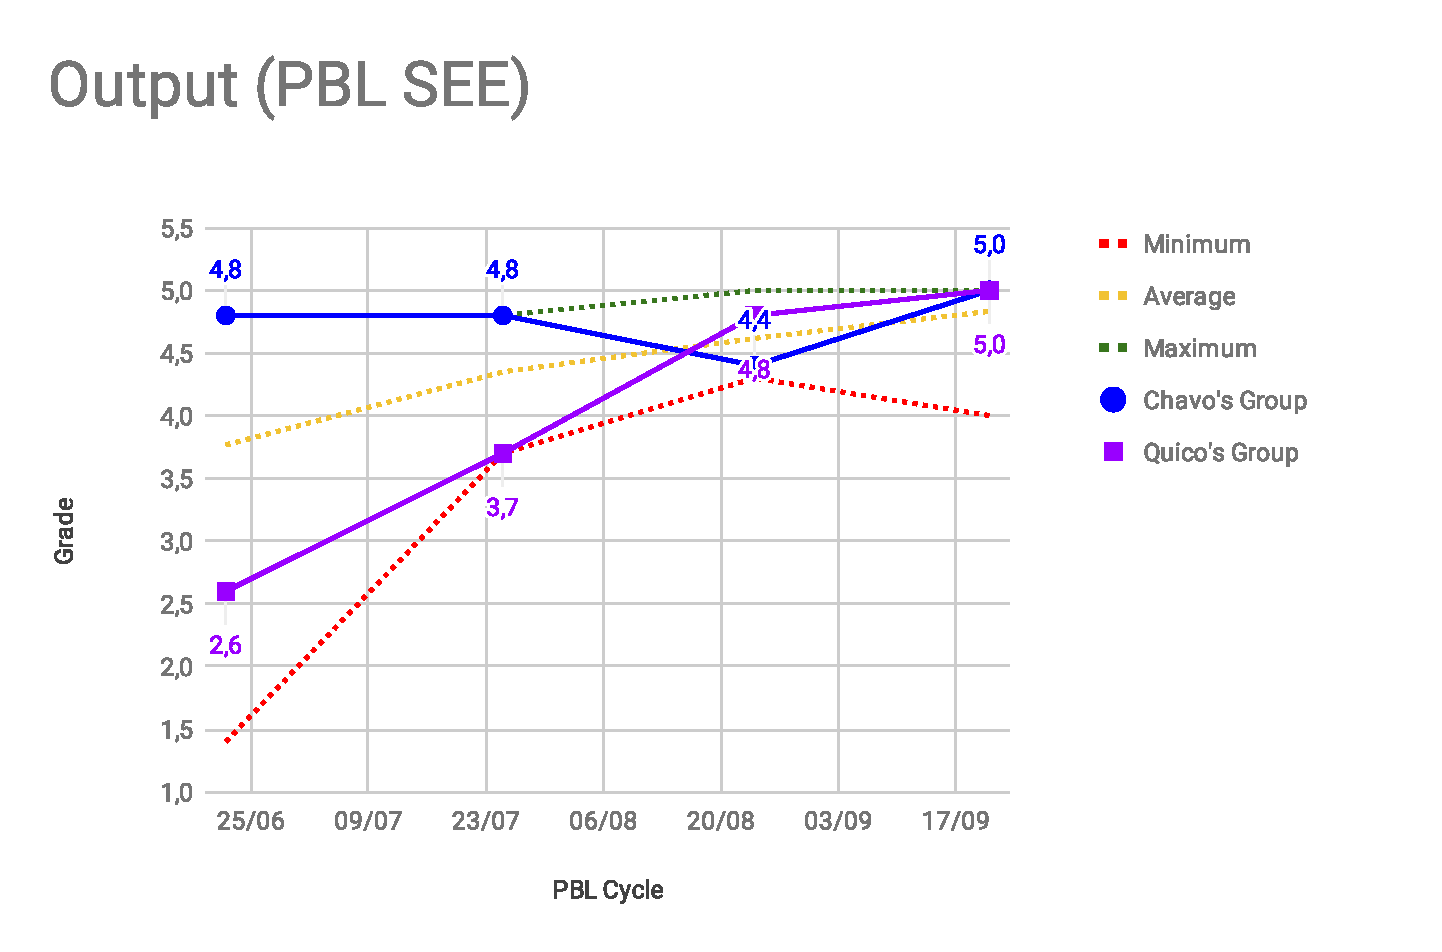
\includegraphics[width=0.9\textwidth]{images/chapter-08/pbl-see_output.pdf}}

\par\medskip\ABNTEXfontereduzida\selectfont\textbf{Source:} Created by the author (2024).
\end{figure}

\begin{figure}[ht!]
\centering

\caption{\textmd{Chart of Client Satisfaction Assessment Perspective (\acrshort{PBL-SEE} Model) for all teams of Chavo's and Quico's class.}}
\label{fig:pbl-see_client-satisfaction}
\fcolorbox{gray}{white}{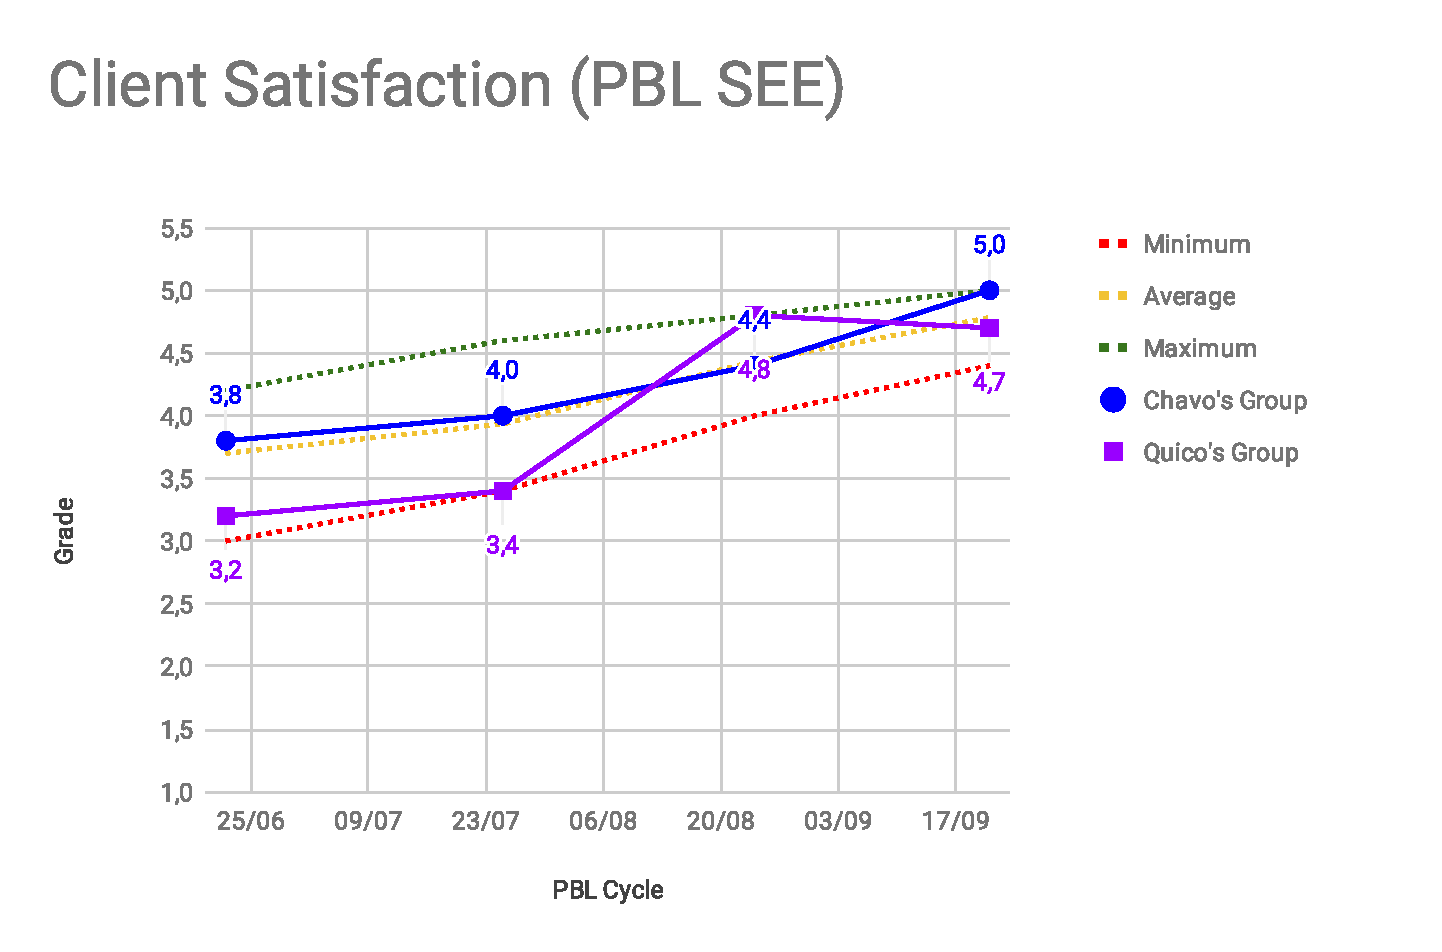
\includegraphics[width=0.9\textwidth]{images/chapter-08/pbl-see_client-satisfaction.pdf}}

\par\medskip\ABNTEXfontereduzida\selectfont\textbf{Source:} Created by the author (2024).
\end{figure}

\begin{figure}[ht!]
\centering

\caption{\textmd{Chart of Performance Assessment Perspective (\acrshort{PBL-SEE} Model) for all students of Chavo's and Quico's class.}}
\label{fig:pbl-see_performance_general}
\fcolorbox{gray}{white}{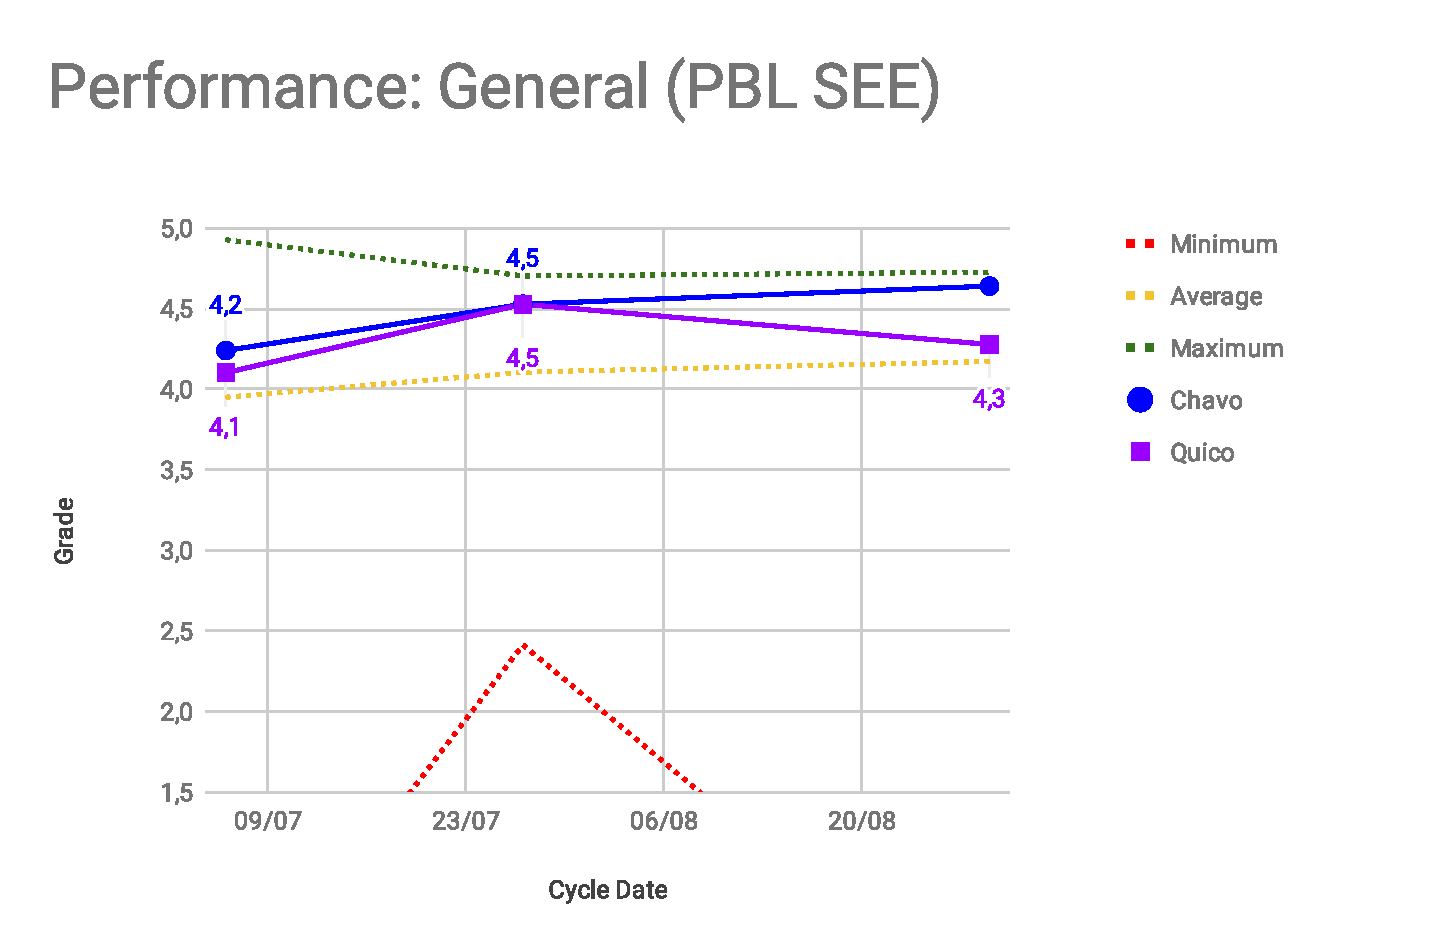
\includegraphics[width=0.9\textwidth]{images/chapter-08/pbl-see_performance_ general.pdf}}

\par\medskip\ABNTEXfontereduzida\selectfont\textbf{Source:} Created by the author (2024).
\end{figure}

\begin{figure}[ht!]
\centering

\caption{\textmd{Chart of Performance Assessment Perspective (\acrshort{PBL-SEE} Model) for all teams of Chavo's and Quico's class.}}
\label{fig:pbl-see_performance_all-teams}
\fcolorbox{gray}{white}{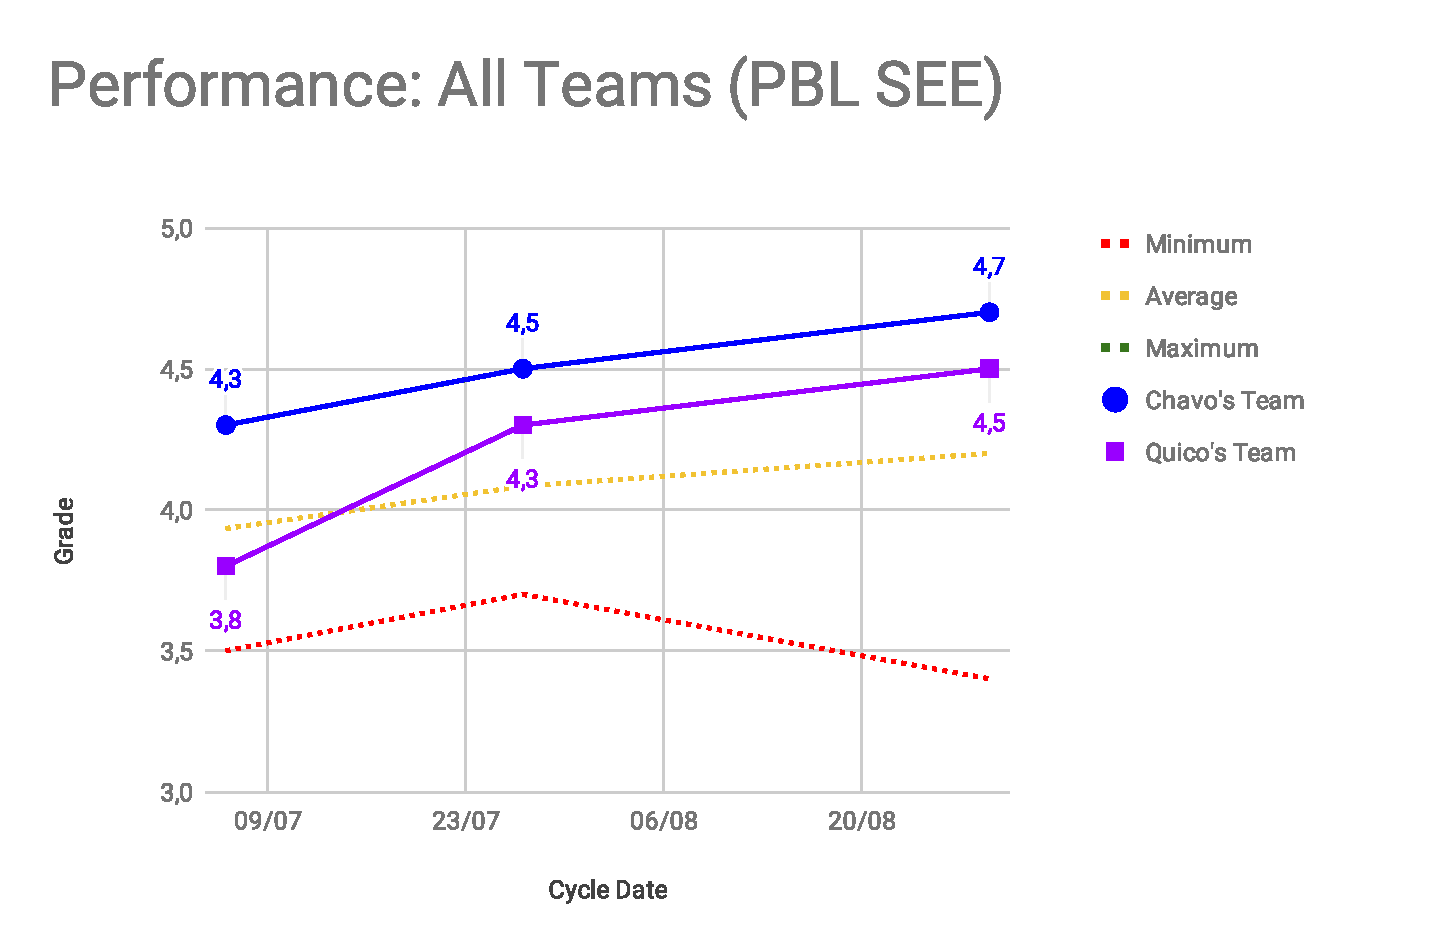
\includegraphics[width=0.9\textwidth]{images/chapter-08/pbl-see_performance_ all-teams.pdf}}

\par\medskip\ABNTEXfontereduzida\selectfont\textbf{Source:} Created by the author (2024).
\end{figure}

\begin{figure}[ht!]
\centering

\caption{\textmd{Chart of Performance Assessment Perspective (\acrshort{PBL-SEE} Model) for all students into Chavo's team.}}
\label{fig:pbl-see_performance_in-chavos-team}
\fcolorbox{gray}{white}{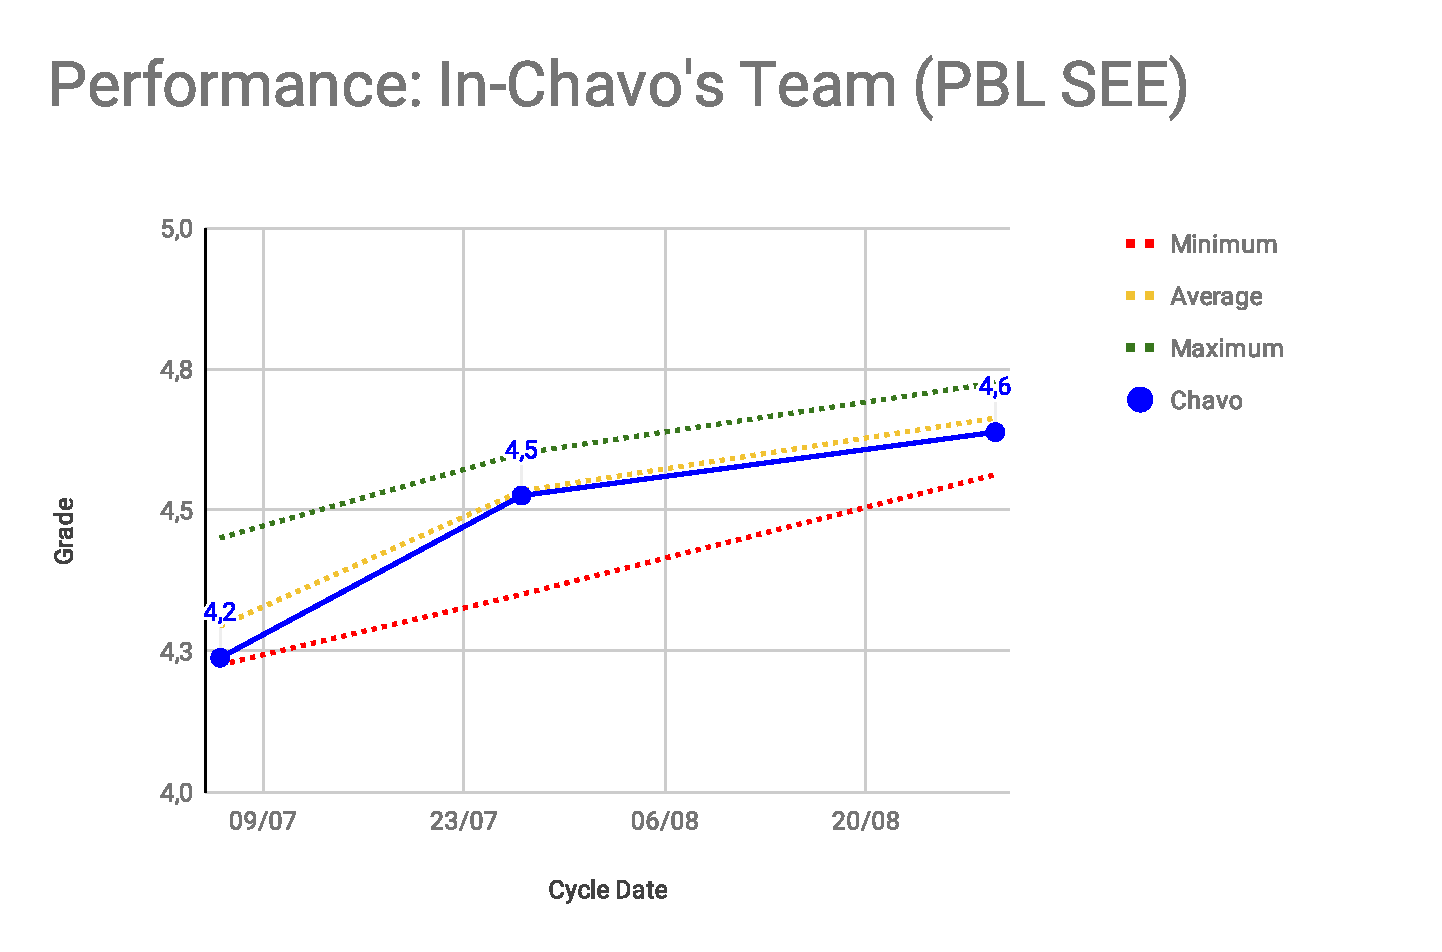
\includegraphics[width=0.9\textwidth]{images/chapter-08/pbl-see_performance_ in-chavos-team.pdf}}

\par\medskip\ABNTEXfontereduzida\selectfont\textbf{Source:} Created by the author (2024).
\end{figure}

\begin{figure}[ht!]
\centering

\caption{\textmd{Chart of Performance Assessment Perspective (\acrshort{PBL-SEE} Model) for all students into Quico's team.}}
\label{fig:pbl-see_performance_in-quicos-team}
\fcolorbox{gray}{white}{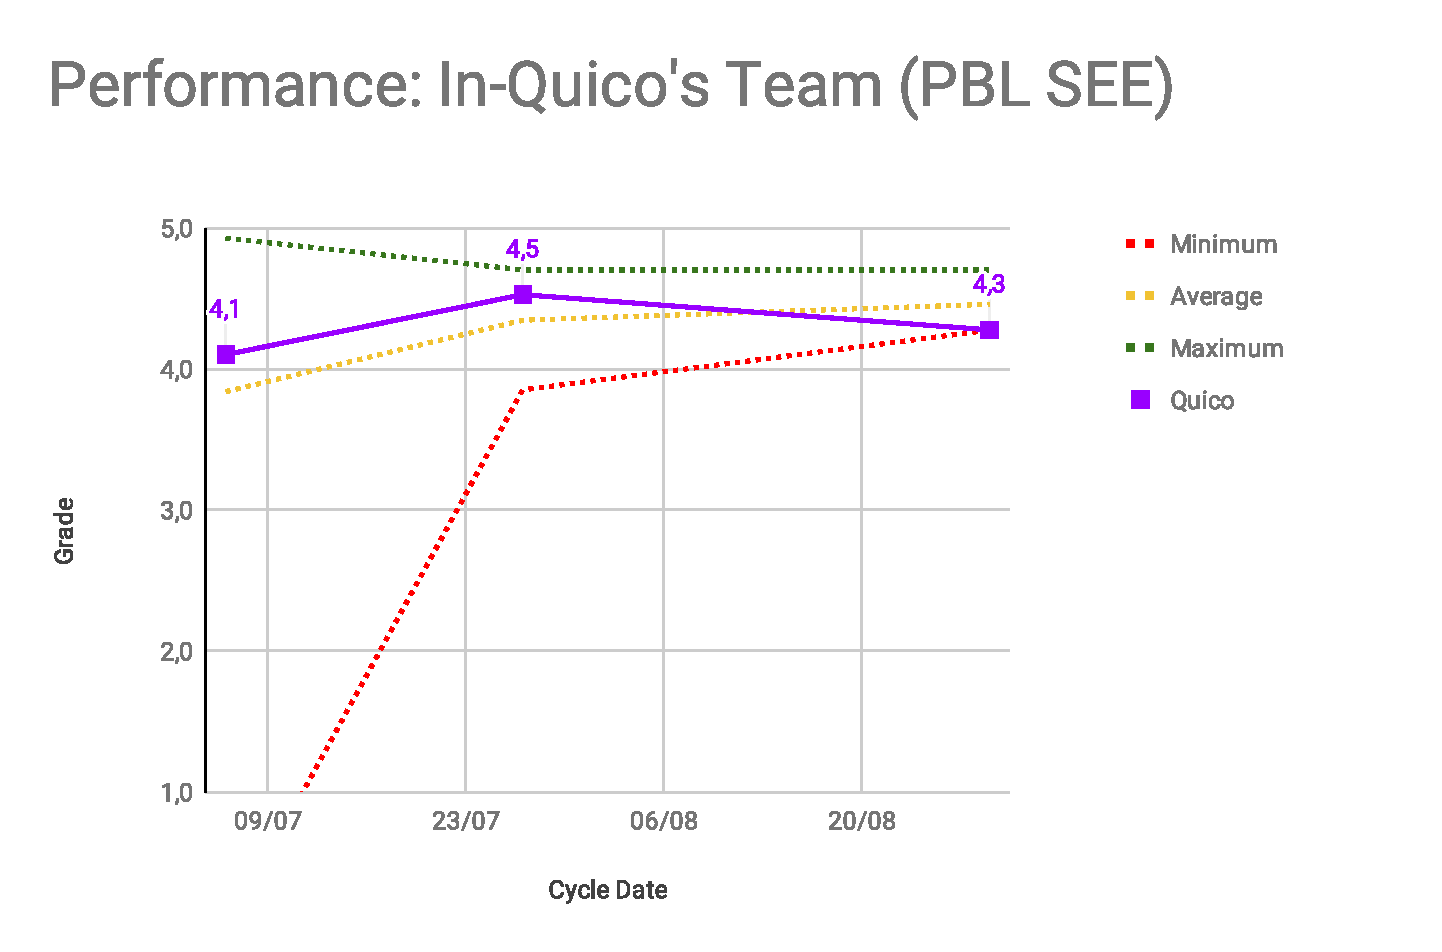
\includegraphics[width=0.9\textwidth]{images/chapter-08/pbl-see_performance_ in-quicos-team.pdf}}

\par\medskip\ABNTEXfontereduzida\selectfont\textbf{Source:} Created by the author (2024).
\end{figure}

\begin{figure}[ht!]
\centering

\caption{\textmd{Chart of Content Assessment Perspective (\acrshort{PBL-SEE} Model) for all students of Chavo's and Quico's class.}}
\label{fig:pbl-see_content_general}
\fcolorbox{gray}{white}{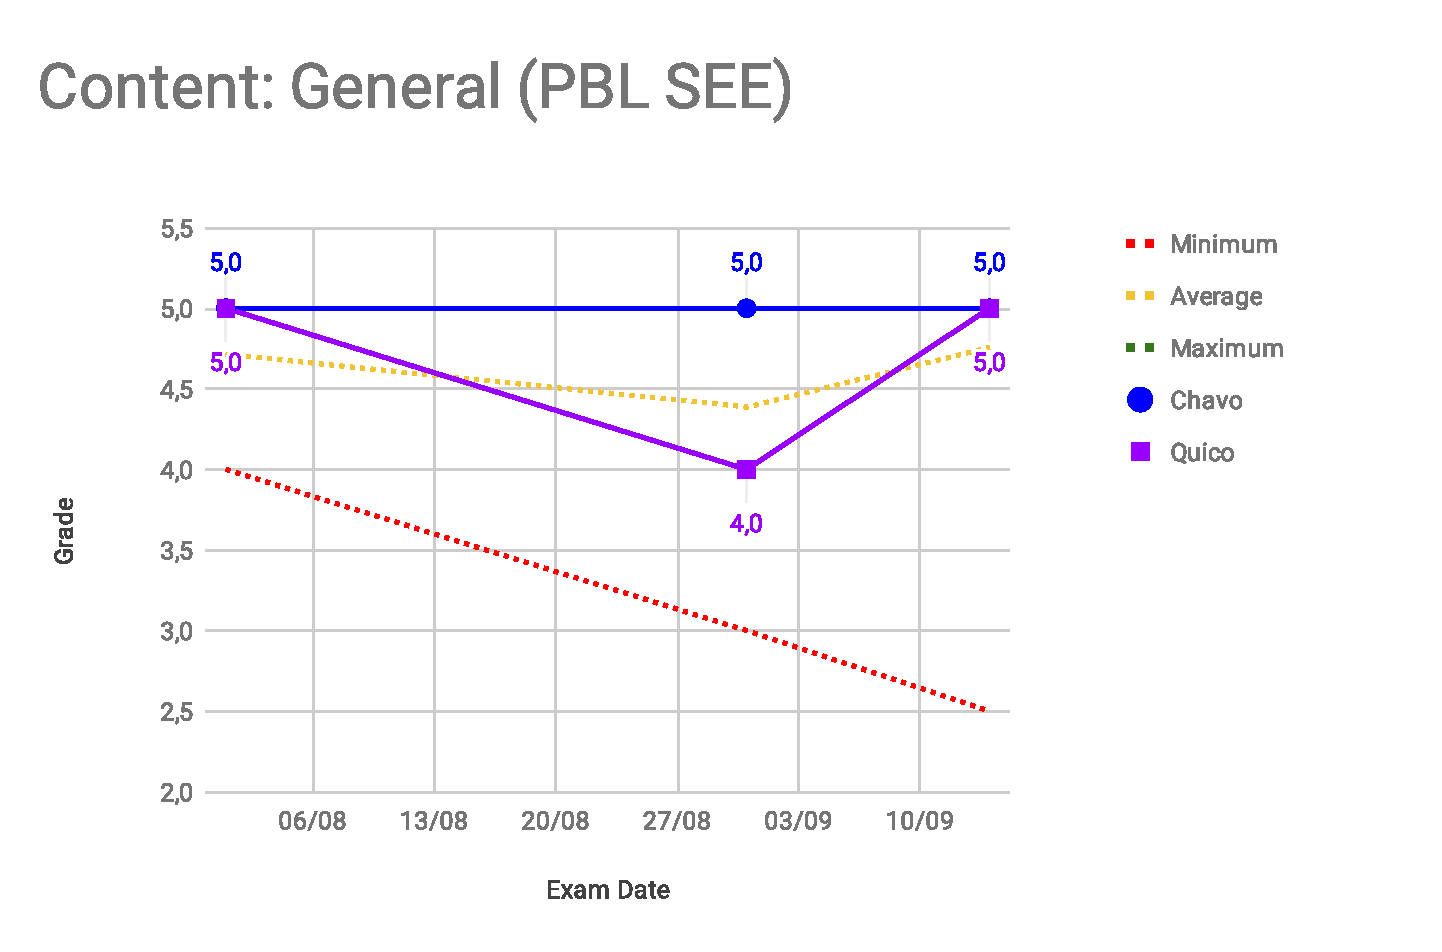
\includegraphics[width=0.9\textwidth]{images/chapter-08/pbl-see_content_ general.pdf}}

\par\medskip\ABNTEXfontereduzida\selectfont\textbf{Source:} Created by the author (2024).
\end{figure}

\begin{figure}[ht!]
\centering

\caption{\textmd{Chart of Content Assessment Perspective (\acrshort{PBL-SEE} Model) for all teams of Chavo's and Quico's class.}}
\label{fig:pbl-see_content_all-teams}
\fcolorbox{gray}{white}{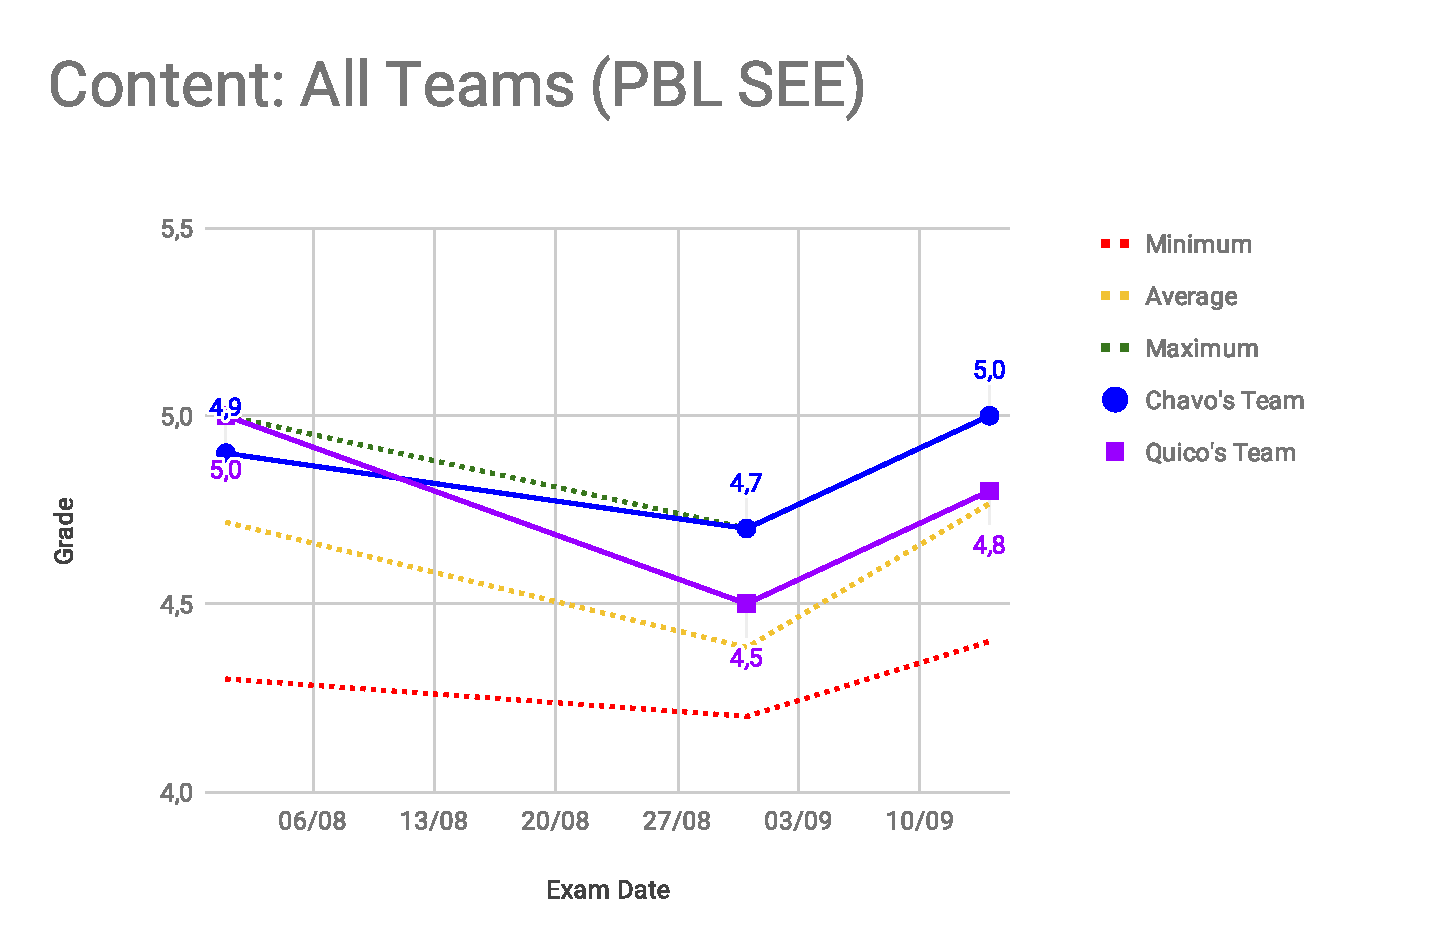
\includegraphics[width=0.9\textwidth]{images/chapter-08/pbl-see_content_ all-teams.pdf}}

\par\medskip\ABNTEXfontereduzida\selectfont\textbf{Source:} Created by the author (2024).
\end{figure}

\begin{figure}[ht!]
\centering

\caption{\textmd{Chart of Content Assessment Perspective (\acrshort{PBL-SEE} Model) for all students into Chavo's team.}}
\label{fig:pbl-see_content_in-chavos-team}
\fcolorbox{gray}{white}{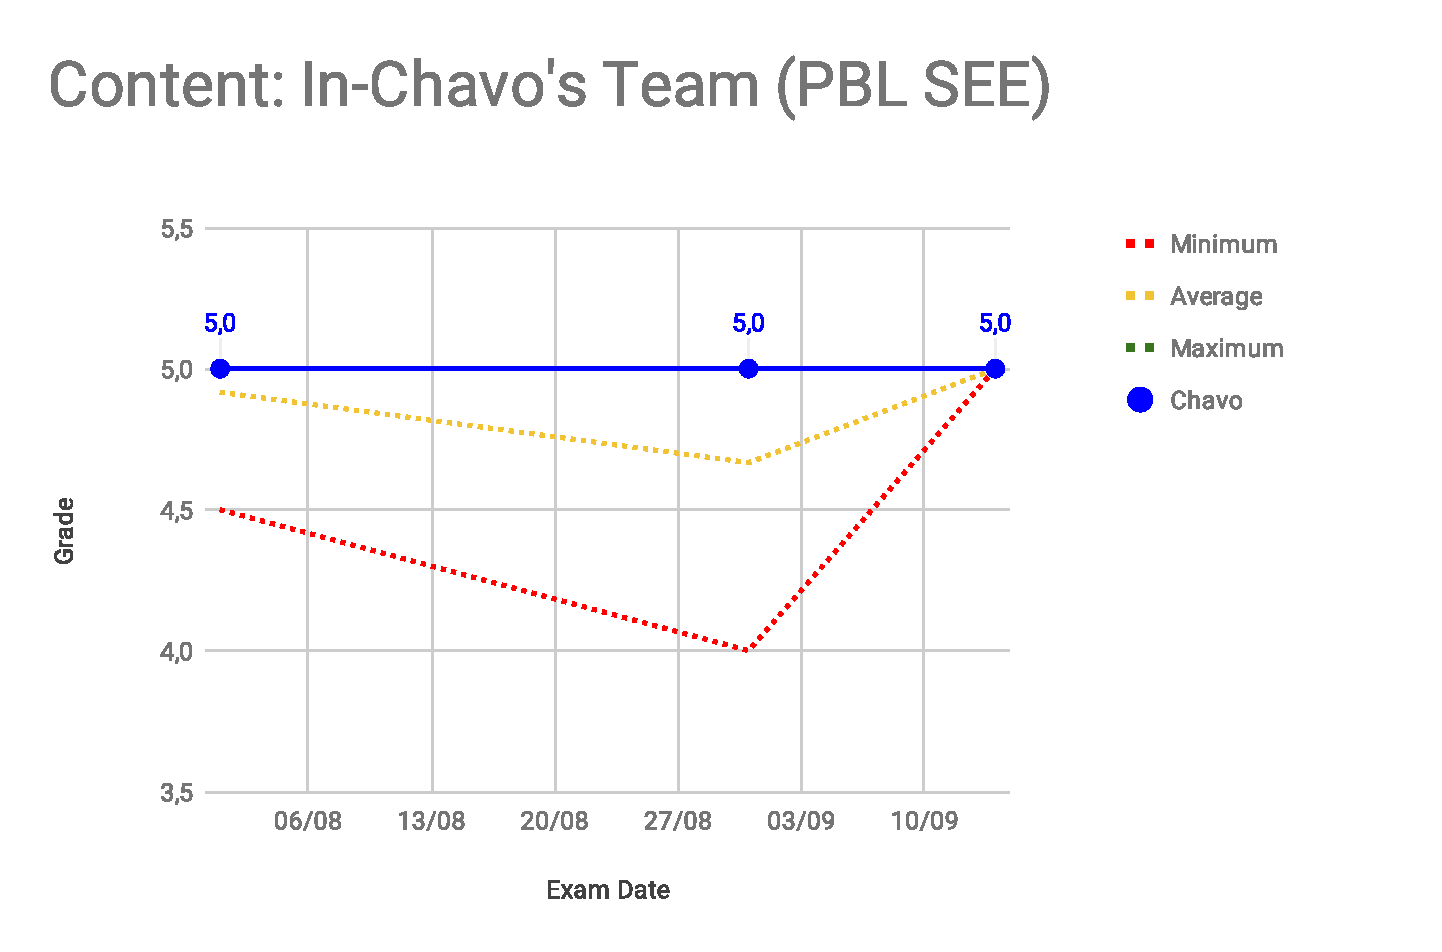
\includegraphics[width=0.9\textwidth]{images/chapter-08/pbl-see_content_ in-chavo's-team.pdf}}

\par\medskip\ABNTEXfontereduzida\selectfont\textbf{Source:} Created by the author (2024).
\end{figure}

\begin{figure}[ht!]
\centering

\caption{\textmd{Chart of Content Assessment Perspective (\acrshort{PBL-SEE} Model) for all students into Quico's team.}}
\label{fig:pbl-see_content_in-quicos-team}
\fcolorbox{gray}{white}{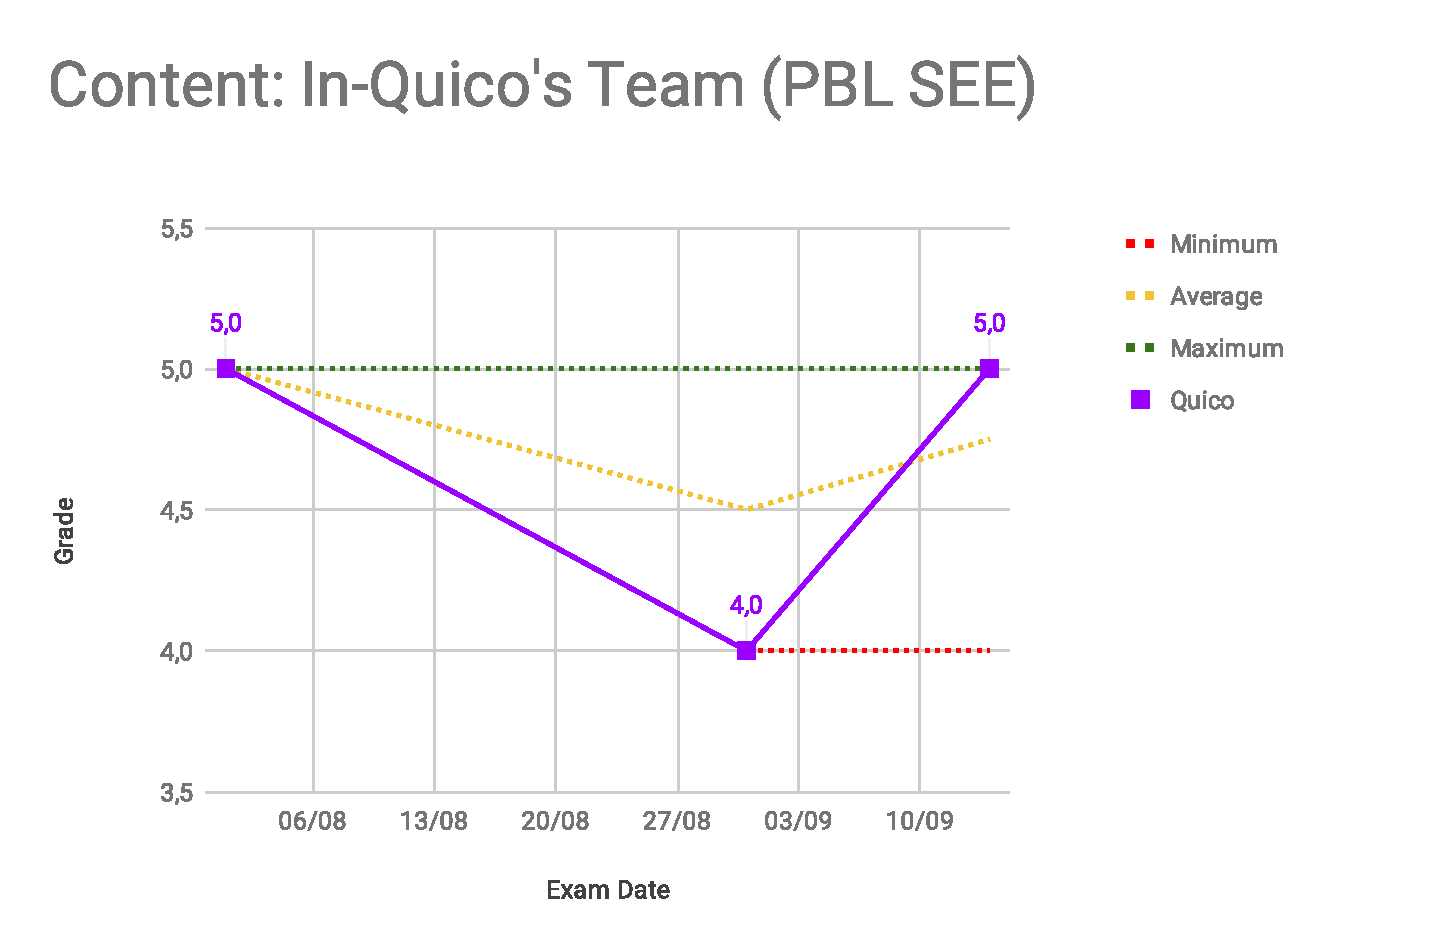
\includegraphics[width=0.9\textwidth]{images/chapter-08/pbl-see_content_ in-quicos-team.pdf}}

\par\medskip\ABNTEXfontereduzida\selectfont\textbf{Source:} Created by the author (2024).
\end{figure}

\begin{figure}[ht!]
\centering

\caption{\textmd{Chart of Process Assessment Perspective (\acrshort{PBL-SEE} Model) for all teams of Chavo's and Quico's class.}}
\label{fig:pbl-see_process}
\fcolorbox{gray}{white}{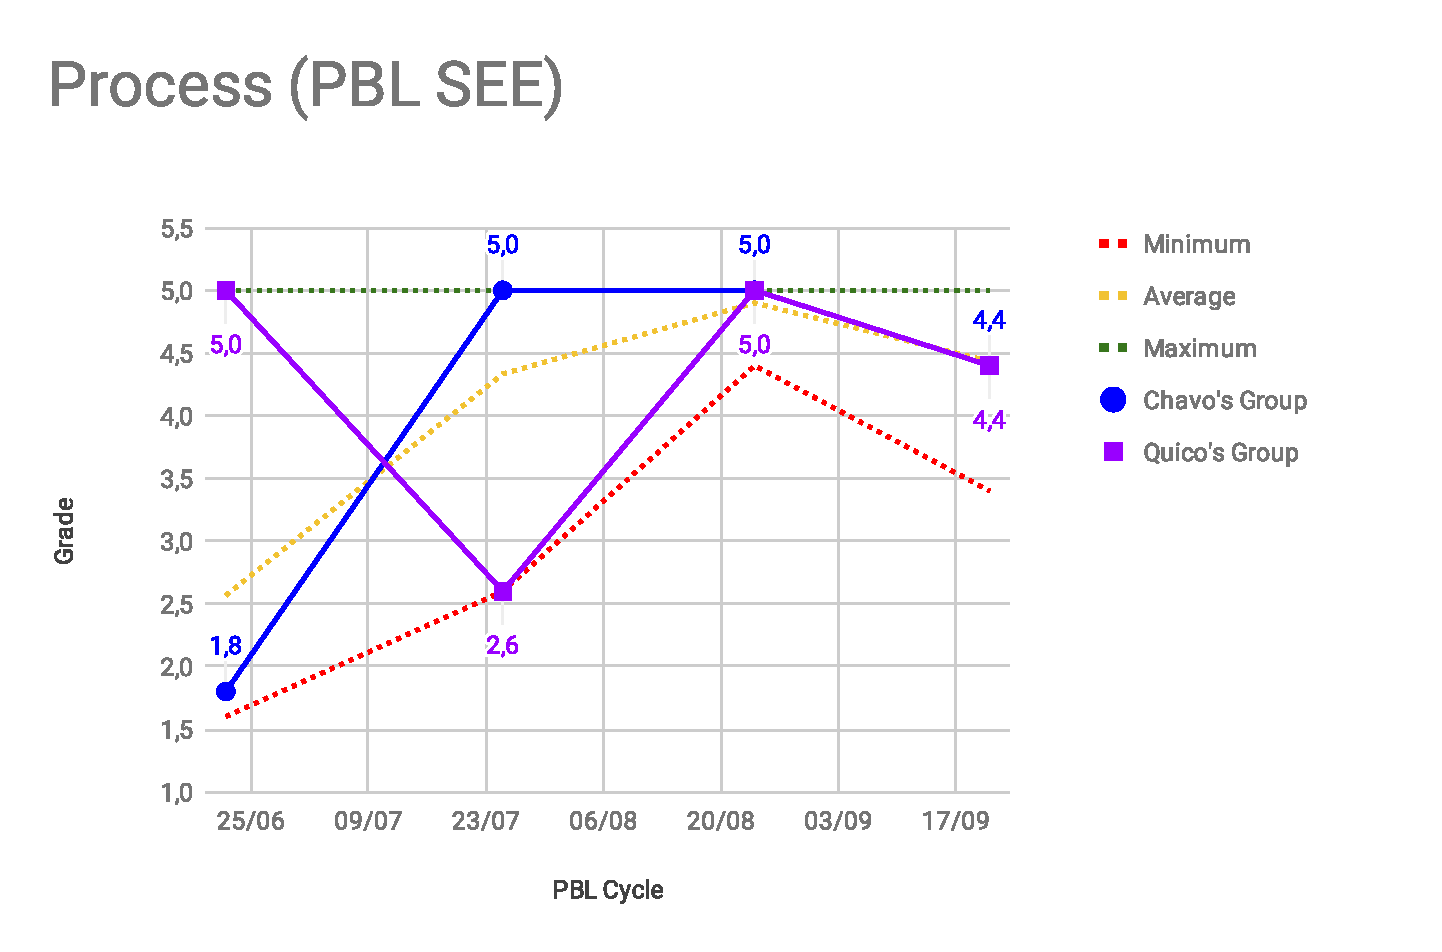
\includegraphics[width=0.9\textwidth]{images/chapter-08/pbl-see_process.pdf}}

\par\medskip\ABNTEXfontereduzida\selectfont\textbf{Source:} Created by the author (2024).
\end{figure}

\addtocontents{toc}{\endgroup}
\end{apendicesenv}




% ----------------------------------------------------------
% Anexos
% ----------------------------------------------------------
%
% ----------------------
% força para que não exiba subtítulos em apêndices no sumário
% -----------------------

\begin{anexosenv}
\addtocontents{toc}{\protect\setcounter{tocdepth}{1}}
\makeatletter
\addtocontents{toc}{%
  \begingroup
  \let\protect\l@chapter\protect\l@section
  \let\protect\l@section\protect\l@subsection
}
\makeatother
% Imprime uma página indicando o início dos apêndices
% \partapendices

%coloca o identificador do anexo/apendice somente na primeira página
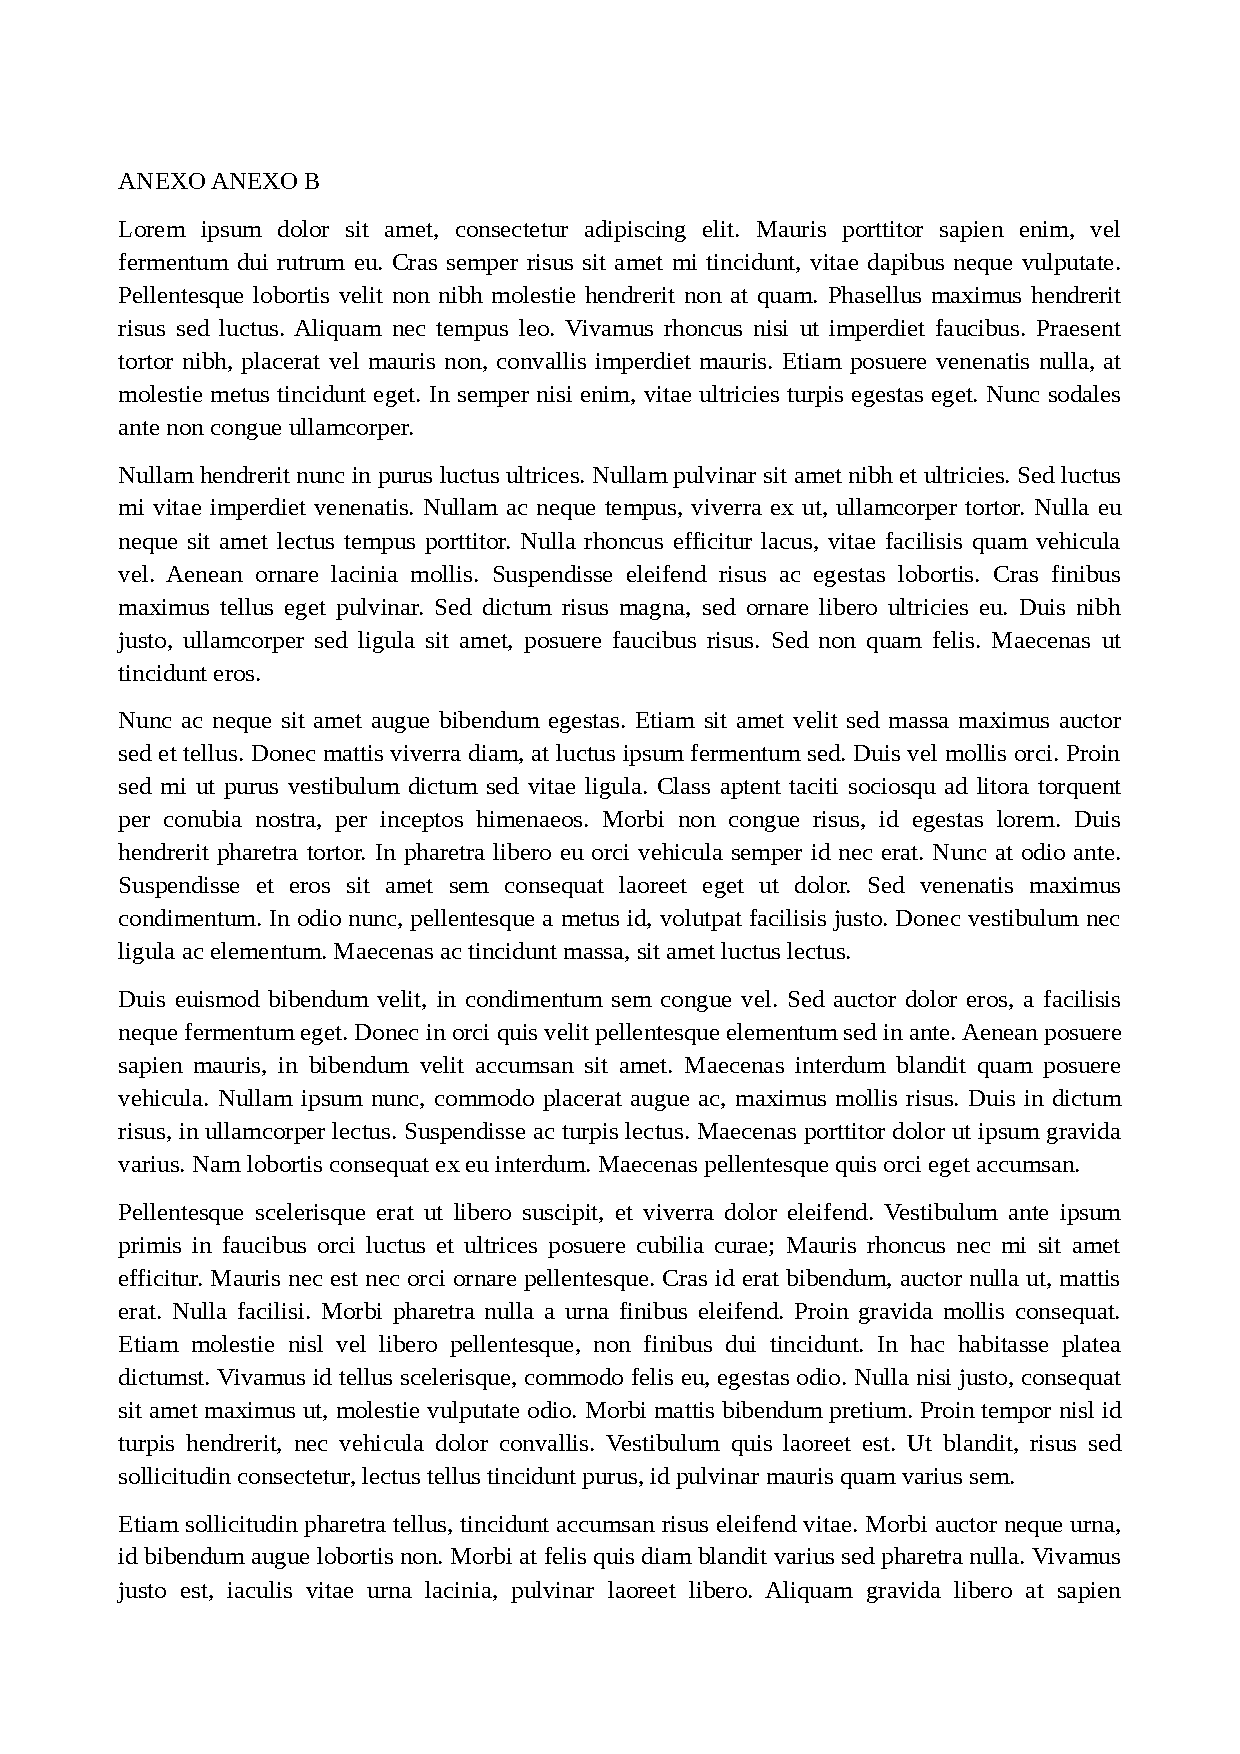
\includepdf[pages={1},scale=0.8,pagecommand=\chapter{Texto Texto Texto Texto}\label{anex:anexob}]{anexos/anexoB}
\includepdf[pages={2-},scale=0.80,pagecommand={}]{anexos/anexoB}

%coloca o identificador do anexo/apendice somente na primeira página
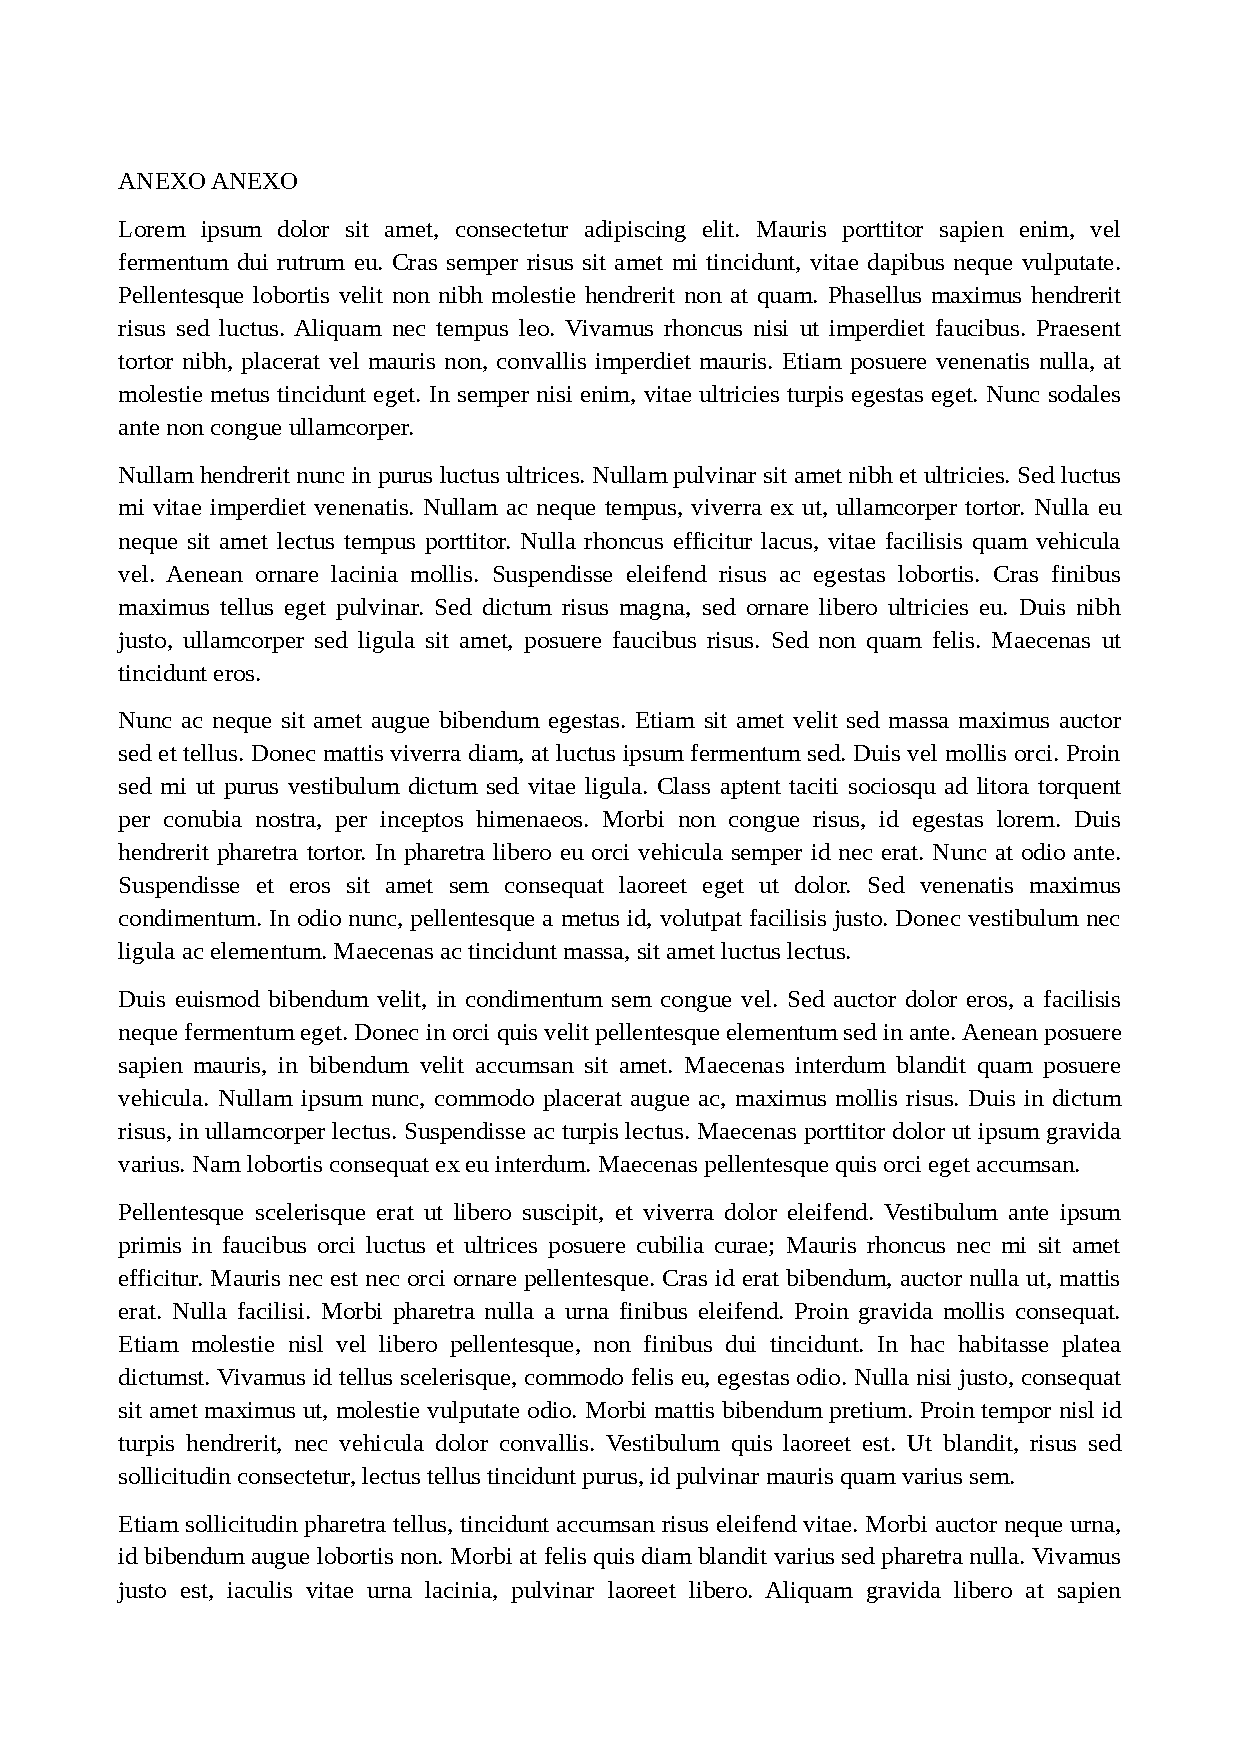
\includepdf[pages={1},scale=0.8,pagecommand=\chapter{Texto Texto Texto Texto}\label{anex:anexoa}]{anexos/anexoA}
\includepdf[pages={2-},scale=0.80,pagecommand={}]{anexos/anexoA}

\addtocontents{toc}{\endgroup}
\end{anexosenv}





\printindex


\end{document}
